%&pdfLaTeX
% !TEX encoding = UTF-8 Unicode
\documentclass[a4paper]{article}
\usepackage{ifxetex}
\ifxetex
\usepackage{fontspec}
\setmainfont[Mapping=tex-text]{STIXGeneral}
\else
\usepackage[T1]{fontenc}
\usepackage[latin1]{inputenc}
\fi
\usepackage{textcomp}

\usepackage{graphicx}
\usepackage{array}
\usepackage{ulem}
\usepackage{fixltx2e}
\usepackage{amssymb}
\usepackage{fancyhdr}
\renewcommand{\headrulewidth}{0pt}
\renewcommand{\footrulewidth}{0pt}

\setlength{\parindent}{0cm}
\setlength{\parskip}{0.18cm}
\usepackage[hmargin=2cm,vmargin=2.5cm,bindingoffset=0.0cm]{geometry}
\usepackage[pdfborder={0 0 0}]{hyperref}
\begin{document}



%&pdfLaTeX
% !TEX encoding = UTF-8 Unicode
\documentclass[a4paper]{article}
\usepackage{ifxetex}
\ifxetex
\usepackage{fontspec}
\setmainfont[Mapping=tex-text]{STIXGeneral}
\else
\usepackage[T1]{fontenc}
\usepackage[latin1]{inputenc}
\fi
\usepackage{textcomp}

\usepackage{graphicx}
\usepackage{array}
\usepackage{ulem}
\usepackage{fixltx2e}
\usepackage{amssymb}
\usepackage{fancyhdr}
\usepackage{amsmath}
\usepackage{algpseudocode}
\usepackage{threeparttable}
\renewcommand{\headrulewidth}{0pt}
\renewcommand{\footrulewidth}{0pt}

\setlength{\parindent}{0cm}
\setlength{\parskip}{0.18cm}
\usepackage[hmargin=2cm,vmargin=2.5cm,bindingoffset=0.0cm]{geometry}
\usepackage[pdfborder={0 0 0}]{hyperref}
\begin{document}



%&pdfLaTeX
% !TEX encoding = UTF-8 Unicode
\documentclass[a4paper]{article}
\usepackage{ifxetex}
\ifxetex
\usepackage{fontspec}
\setmainfont[Mapping=tex-text]{STIXGeneral}
\else
\usepackage[T1]{fontenc}
\usepackage[latin1]{inputenc}
\fi
\usepackage{textcomp}

\usepackage{graphicx}
\usepackage{array}
\usepackage{ulem}
\usepackage{fixltx2e}
\usepackage{amssymb}
\usepackage{fancyhdr}
\usepackage{amsmath}
\usepackage{algpseudocode}
\usepackage{threeparttable}
\renewcommand{\headrulewidth}{0pt}
\renewcommand{\footrulewidth}{0pt}

\setlength{\parindent}{0cm}
\setlength{\parskip}{0.18cm}
\usepackage[hmargin=2cm,vmargin=2.5cm,bindingoffset=0.0cm]{geometry}
\usepackage[pdfborder={0 0 0}]{hyperref}
\begin{document}



%&pdfLaTeX
% !TEX encoding = UTF-8 Unicode
\documentclass[a4paper]{article}
\usepackage{ifxetex}
\ifxetex
\usepackage{fontspec}
\setmainfont[Mapping=tex-text]{STIXGeneral}
\else
\usepackage[T1]{fontenc}
\usepackage[latin1]{inputenc}
\fi
\usepackage{textcomp}

\usepackage{graphicx}
\usepackage{array}
\usepackage{ulem}
\usepackage{fixltx2e}
\usepackage{amssymb}
\usepackage{fancyhdr}
\usepackage{amsmath}
\usepackage{algpseudocode}
\usepackage{threeparttable}
\renewcommand{\headrulewidth}{0pt}
\renewcommand{\footrulewidth}{0pt}

\setlength{\parindent}{0cm}
\setlength{\parskip}{0.18cm}
\usepackage[hmargin=2cm,vmargin=2.5cm,bindingoffset=0.0cm]{geometry}
\usepackage[pdfborder={0 0 0}]{hyperref}
\begin{document}



\input{CRAMv3.ver}
\title{CRAM format specification (version 3.0)}
\author{samtools-devel@lists.sourceforge.net}
\date{\headdate}
\maketitle


\begin{quote}\small
The master version of this document can be found at
\url{https://github.com/samtools/hts-specs}.\\
This printing is version~\commitdesc\ from that repository,
last modified on the date shown above.
\end{quote}

\begin{center}
\textit{license: Apache 2.0}
\end{center}
\vspace*{1em}

\section{\textbf{Overview}}

This specification describes the CRAM 3.0 format. 

CRAM has the following major objectives:

\begin{enumerate}
\item Significantly better lossless compression than BAM

\item Full compatibility with BAM

\item Effortless transition to CRAM from using BAM files

\item Support for controlled loss of BAM data
\end{enumerate}

The first three objectives allow users to take immediate advantage of the CRAM 
format while offering a smooth transition path from using BAM files. The fourth 
objective supports the exploration of different lossy compression strategies and 
provides a framework in which to effect these choices. Please note that the CRAM 
format does not impose any rules about what data should or should not be preserved. 
Instead, CRAM supports a wide range of lossless and lossy data preservation strategies 
enabling users to choose which data should be preserved.

Data in CRAM is stored either as CRAM records or using one of the general purpose 
compressors (gzip, bzip2). CRAM records are compressed using a number of different 
encoding strategies. For example, bases are reference compressed (\emph{Hsi-Yang 
Fritz, et al. (2011) Genome Res. 21:734-740}) by encoding base differences rather 
than storing the bases themselves.

\section{\textbf{Data types}}

CRAM specification uses logical data types and storage data types; logical data 
types are written as words (e.g. int) while physical data types are written using 
single letters (e.g. i). The difference between the two is that storage data types 
define how logical data types are stored in CRAM. Data in CRAM is stored either 
as bits or bytes. Writing values as bits and bytes is described in detail 
below.

\subsection{\textbf{Logical data types}}

\begin{description}
\item[Byte]\ \newline
Signed byte (8 bits).

\item[Integer]\ \newline
Signed 32-bit integer. 

\item[Long]\ \newline
Signed 64-bit integer. 

\item[Array]\ \newline
An array of any logical data type: \texttt{<}type\texttt{>}[ ] 
\end{description}

% \begin{tabular}{ll}
% \textbf{Byte}    & Signed byte (8 bits).  \\
% \\
% \textbf{Integer} & Signed 32-bit integer. \\
% \\
% \textbf{Long}    & Signed 64-bit integer. \\
% \\
% \textbf{Array}   & An array of any logical data type: \texttt{<}type\texttt{>}[ ] \\
% \end{tabular}

\subsection{\textbf{Writing bits to a bit stream}}

A bit stream consists of a sequence of 1s and 0s. The bits are written most significant 
bit first where new bits are stacked to the right and full bytes on the left are 
written out. In a bit stream the last byte will be incomplete if less than 8 bits 
have been written to it. In this case the bits in the last byte are shifted to 
the left.

\subsubsection*{Example of writing to bit stream}

Let's consider the following example. The table below shows a sequence of write 
operations: 

\begin{tabular}{|l|l|l|l|l|}
\hline
\textbf{Operation order} & \textbf{Buffer state before} & \textbf{Written bits} & \textbf{Buffer state after} & \textbf{Issued bytes}\tabularnewline
\hline
1 & 0x0 & 1 & 0x1 & -\tabularnewline
\hline
2 & 0x1 & 0 & 0x2 & -\tabularnewline
\hline
3 & 0x2 & 11 & 0xB & -\tabularnewline
\hline
4 & 0xB & 0000 0111 & 0x7 & 0xB0\tabularnewline
\hline
\end{tabular}

After flushing the above bit stream the following bytes are written: 0xB0 0x70. 
Please note that the last byte was 0x7 before shifting to the left and became 0x70 
after that:

\texttt{> echo "obase=16; ibase=2; 00000111" \textbar{} bc\\
7\\
\\
> echo "obase=16; ibase=2; 01110000" \textbar{} bc\\
70}

And the whole bit sequence: 

\texttt{> echo "obase=2; ibase=16; B070" \textbar{} bc\\
1011000001110000}

When reading the bits from the bit sequence it must be known that only 12 bits 
are meaningful and the bit stream should not be read after that. 

\subsubsection*{Note on writing to bit stream}

When writing to a bit stream both the value and the number of bits in the value 
must be known. This is because programming languages normally operate with bytes 
(8 bits) and to specify which bits are to be written requires a bit-holder, for 
example an integer, and the number of bits in it. Equally, when reading a value 
from a bit stream the number of bits must be known in advance. In case of prefix 
codes (e.g. Huffman) all possible bit combinations are either known in advance 
or it is possible to calculate how many bits will follow based on the first few 
bits. Alternatively, two codes can be combined, where the first contains the number 
of bits to read. 

\subsection{\textbf{Writing bytes to a byte stream}}
\label{subsec:writing-bytes}

The interpretation of byte stream is straightforward. CRAM uses little \emph{endianness} 
for bytes when applicable and defines the following storage data types:

\begin{description}

\item[Boolean (bool)]\ \newline
Boolean is written as 1-byte with 0x0 being `false' and 0x1 being `true'.

\item[Integer (int32)]\ \newline
Signed 32-bit integer, written as 4 bytes in little-endian byte order.

\item[Long (int64)]\ \newline
Signed 64-bit integer, written as 8 bytes in little-endian byte order.

\item[ITF-8 integer (itf8)]\ \newline
This is an alternative way to write an integer value. The idea is similar to UTF-8 
encoding and therefore this encoding is called ITF-8 (Integer Transformation Format 
- 8 bit). 

The most significant bits of the first byte have special meaning and are called 
`prefix'. These are 0 to 4 true bits followed by a 0. The number of 1's denote 
the number of bytes to follow. To accommodate 32 bits such representation requires 
5 bytes with only 4 lower bits used in the last byte 5.

\item[LTF-8 long (ltf8)]\ \newline
See ITF-8 for more details. The only difference between ITF-8 and LTF-8 is the 
number of bytes used to encode a single value. To do so 64 bits are required and 
this can be done with 9 byte at most with the first byte consisting of just 1s 
or 0xFF value. 

\item[{Array ([ ])}]\ \newline
Array length is written first as integer (itf8), followed by the elements of the 
array. 

\item[{Encoding}]\ \newline
Encoding is a data type that specifies how data series have been compressed. Encodings 
are defined as encoding\texttt{<}type\texttt{>} where the type is a logical data 
type as opposed to a storage data type.

An encoding is written as follows. The first integer (itf8) denotes the codec id 
and the second integer (itf8) the number of bytes in the following encoding-specific 
values. 

Subexponential encoding example: 

\begin{tabular}{|l|l|l|}
\hline
\textbf{Value} & \textbf{Type} & \textbf{Name}\tabularnewline
\hline
0x7 & itf8 & codec id\tabularnewline
\hline
0x2 & itf8 & number of bytes to follow\tabularnewline
\hline
0x0 & itf8 & offset\tabularnewline
\hline
0x1 & itf8 & K parameter\tabularnewline
\hline
\end{tabular}

The first byte ``0x7'' is the codec id. 

The next byte ``0x2'' denotes the length of the bytes to follow (2). 

The subexponential encoding has 2 parameters: integer (itf8) offset and integer (itf8) K.

offset = 0x0 = 0

K = 0x1 = 1


\item[{Map}]\ \newline
A map is a collection of keys and associated values. A map with N keys is written 
as follows: 

\begin{tabular}{|l|l|l|l|l|l|l|l|}
\hline
size in bytes & N & key 1 & value 1 & key ... & value ... & key N & value N\tabularnewline
\hline
\end{tabular}

Both the size in bytes and the number of keys are written as integer (itf8). Keys 
and values are written according to their data types and are specific to each map.

\item[String]\ \newline
A string is represented as byte arrays using UTF-8 format. Read names, reference 
sequence names and tag values with type `Z' are stored as UTF-8.

\end{description}


\section{\textbf{Encodings }}

Encoding is a data structure that captures information about compression details 
of a data series that are required to uncompress it. This could be a set of constants 
required to initialize a specific decompression algorithm or statistical properties 
of a data series or, in case of data series being stored in an external block, 
the block content id. 

Encoding notation is defined as the keyword `encoding' followed by its data type 
in angular brackets, for example `encoding\texttt{<}byte\texttt{>}' stands for 
an encoding that operates on a data series of data type `byte'. 

Encodings may have parameters of different data types, for example the external 
encoding has only one parameter, integer id of the external block. The following 
encodings are defined: 

\begin{tabular}{|l|l|>{\raggedright}p{155pt}|>{\raggedright}p{160pt}|}
\hline
\textbf{Codec} & \textbf{ID} & \textbf{Parameters} & \textbf{Comment}\tabularnewline
\hline
NULL & 0 & none & series not preserved\tabularnewline
\hline
EXTERNAL & 1 & int block content id & the block content identifier used to associate 
external data blocks with data series\tabularnewline
\hline
Deprecated (GOLOMB) & 2 & int offset, int M & Golomb coding\tabularnewline
\hline
HUFFMAN & 3 & int array, int array & coding with int/byte values\tabularnewline
\hline
BYTE\_ARRAY\_LEN & 4 & encoding\texttt{<}int\texttt{>} array length, encoding\texttt{<}byte\texttt{>} 
bytes & coding of byte arrays with array length\tabularnewline
\hline
BYTE\_ARRAY\_STOP & 5 & byte stop, int external block\linebreak{}
content id & coding of byte arrays with a stop value \tabularnewline
\hline
BETA & 6 & int offset, int number of bits & binary coding\tabularnewline
\hline
SUBEXP & 7 & int offset, int K & subexponential coding\tabularnewline
\hline
Deprecated (GOLOMB\_RICE) & 8 & int offset, int log$_{\text{2}}$m & Golomb-Rice coding\tabularnewline
\hline
GAMMA & 9 & int offset & Elias gamma coding\tabularnewline
\hline
\end{tabular}

A more detailed description of all the above coding algorithms and their parameters 
can be found in the \emph{Codings }section. 

\section{\textbf{Checksums}}
The checksumming is used to ensure data integrity. The following checksumming algorithms are used in CRAM.
\subsection{\textbf{CRC32}}
This is a cyclic redundancy checksum 32-bit long with the polynomial 0x04C11DB7. Please refer to \href{http://www.itu.int/rec/recommendation.asp?type=folders&lang=e&parent=T-REC-V.42}{ITU-T V.42} for more details. The value of the CRC32 hash function is written as an integer.
\subsection{\textbf{CRC32 sum}}
CRC32 sum is a combination of CRC32 values by summing up all individual CRC32 values modulo 2\textsuperscript{32}. 

\section{\textbf{File structure}}

The overall CRAM file structure is described in this section. Please refer to other 
sections of this document for more detailed information. 

A CRAM file starts with a fixed length file definition followed by one or more 
containers. The BAM header is stored in the first container.

%%\begin{figure}[htbp]
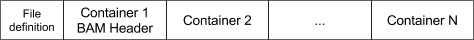
\includegraphics[width=356pt, height=31pt, keepaspectratio=true]{img/CRAMFileFormat2-1-fig001.png}
%%\caption{This should be the caption for \texttt{img/CRAMFileFormat2-1-fig001.png}.}
%%\end{figure}

Pic.1 CRAM file starts with a file definition followed by the BAM header and other 
containers.

Containers consist of one or more blocks. By convention, the BAM header is stored 
in the first container within a single block. This is known as the BAM header block.

%%\begin{figure}[htbp]
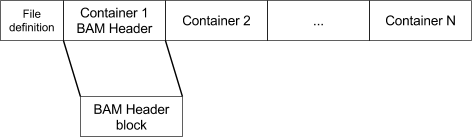
\includegraphics[width=354pt, height=103pt, keepaspectratio=true]{img/CRAMFileFormat2-1-fig002.png}
%%\caption{This should be the caption for \texttt{img/CRAMFileFormat2-1-fig002.png}.}
%%\end{figure}

Pic.2 The BAM header is stored in the first container.

Each container starts with a container header followed by one or more blocks. Each 
block starts with a block header. All data in CRAM is stored within blocks after 
the block header.

%%\begin{figure}[htbp]
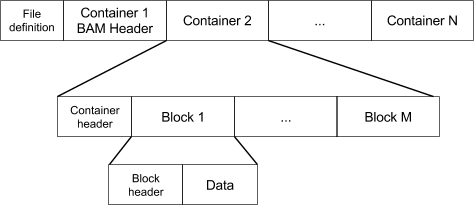
\includegraphics[width=356pt, height=154pt, keepaspectratio=true]{img/CRAMFileFormat2-1-fig003.png}
%%\caption{This should be the caption for \texttt{img/CRAMFileFormat2-1-fig003.png}.}
%%\end{figure}

Pic.3 Container and block structure. All data in CRAM files is stored in blocks.

The first block in each container is the compression header block:

%%\begin{figure}[htbp]
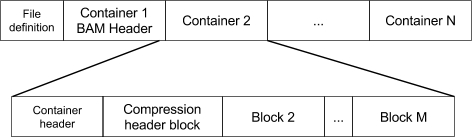
\includegraphics[width=354pt, height=103pt, keepaspectratio=true]{img/CRAMFileFormat2-1-fig004.png}
%%\caption{This should be the caption for \texttt{img/CRAMFileFormat2-1-fig004.png}.}
%%\end{figure}

Pic.4 Compression header is the first block in the container.

The blocks after the compression header are organised logically into slices. One 
slice may contain, for example, a contiguous region of alignment data. Slices begin 
with a slice header block and are followed by one or more data blocks:

%%\begin{figure}[htbp]
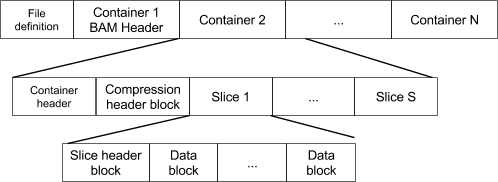
\includegraphics[width=374pt, height=137pt, keepaspectratio=true]{img/CRAMFileFormat2-1-fig005.png}
%%\caption{This should be the caption for \texttt{img/CRAMFileFormat2-1-fig005.png}.}
%%\end{figure}

Pic.5 Containers are logically organised into slices.

Data blocks are divided into core and external data blocks. Each slice must have 
at least one core data block immediately after the slice header block. The core 
data block may be followed by one or more external data blocks.

%%\begin{figure}[htbp]
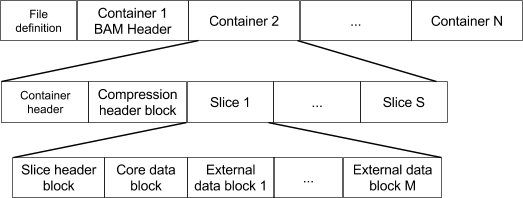
\includegraphics[width=392pt, height=149pt, keepaspectratio=true]{img/CRAMFileFormat2-1-fig006.png}
%%\caption{This should be the caption for \texttt{img/CRAMFileFormat2-1-fig006.png}.}
%%\end{figure}

Pic.5 Data blocks are divided into core and external data blocks. 

\section{\textbf{File definition}}

Each CRAM file starts with a fixed length (26 bytes) definition with the following 
fields:

\begin{tabular}{|l|l|l|}
\hline
\textbf{Data type} & \textbf{Name} & \textbf{Value}\tabularnewline
\hline
byte[4] & format magic number & CRAM (0x43 0x52 0x41 0x4d)\tabularnewline
\hline
unsigned byte & major format number & 3 (0x3)\tabularnewline
\hline
unsigned byte & minor format number & 0 (0x0)\tabularnewline
\hline
byte[20] & file id & CRAM file identifier (e.g. file name or SHA1 checksum)\tabularnewline
\hline
\end{tabular}

Valid CRAM \textit{major}.\textit{minor} version numbers are as follows:

\begin{itemize}
\item[\textit{1.0}]
The original public CRAM release.

\item[\textit{2.0}]
The first CRAM release implemented in both Java and C; tidied up
implementation vs specification differences in \textit{1.0}.

\item[\textit{2.1}]
Gained end of file markers; compatible with \textit{2.0}.

\item[\textit{3.0}]
Additional compression methods; header and data checksums;
improvements for unsorted data.
\end {itemize}

\section{\textbf{Container structure}}

The file definition is followed by one or more containers with the following header 
structure where the container content is stored in the `blocks' field:

\begin{tabular}{|l|>{\raggedright}p{120pt}|>{\raggedright}p{260pt}|}
\hline
\textbf{Data type} & \textbf{Name} & \textbf{Value}
\tabularnewline
\hline
int32 & length & byte size of the container data (blocks)\tabularnewline
\hline
itf8 & reference sequence id & reference sequence identifier  or\linebreak{}
-1 for unmapped reads\linebreak{}
-2 for multiple reference sequences\tabularnewline
\hline
itf8 & starting position on the reference & the alignment start position or\linebreak{}
0 for unmapped reads\tabularnewline
\hline
itf8 & alignment span & the length of the alignment or\linebreak{}
0 for unmapped reads\tabularnewline
\hline
itf8 & number of records & number of records in the container\tabularnewline
\hline
ltf8 & record counter & 1-based sequential index of records in the file/stream.\tabularnewline
\hline
ltf8 & bases & number of read bases\tabularnewline
\hline
itf8 & number of blocks & the number of blocks\tabularnewline
\hline
itf8[ ] & landmarks & Each integer value of this array is a byte offset into the 
blocks byte array. Landmarks are used for random access indexing.\tabularnewline
\hline
int & crc32 & CRC32 hash of the all the preceding bytes in the container.\tabularnewline
\hline
byte[ ] & blocks & The blocks contained within the container.\tabularnewline
\hline
\end{tabular}

\subsection{\textbf{CRAM header in the first container}}

The first container in the CRAM file contains the BAM header in an optionally
compressed block. Only gzip is allowed as compression method for this block. BAM
header is terminated with \textbackslash{}0 byte and any extra bytes in the
block can be used to expand the BAM header. For example when updating @SQ
records additional space may be required for the BAM header. It is recommended
to reserve 50\% more space in the CRAM header block than it is required by the
BAM header.

\section{\textbf{Block structure}}

Containers consist of one or more blocks. Block compression is applied independently 
and in addition to any encodings used to compress data within the block. The block 
have the following header structure with the data stored in the `block data' field:

\begin{tabular}{|l|>{\raggedright}p{120pt}|>{\raggedright}p{260pt}|}
\hline
\textbf{Data type} & \textbf{Name} & \textbf{Value}
\tabularnewline
\hline
byte & method & the block compression method: \linebreak{}
0: raw (none)*\linebreak{}
1: gzip\linebreak{}
2: bzip2\linebreak{}
3: lzma\linebreak{}
4: rans\tabularnewline
\hline
byte & block content type id & the block content type identifier\tabularnewline
\hline
itf8 & block content id & the block content identifier used to associate external 
data blocks with data series\tabularnewline
\hline
itf8 & size in bytes* & size of the block data after applying block compression\tabularnewline
\hline
itf8 & raw size in bytes* & size of the block data before applying block compression\tabularnewline
\hline
byte[ ] & block data & the data stored in the block:\linebreak{}
$\bullet$ bit stream of CRAM records (core data block)\linebreak{}
$\bullet$ byte stream (external data block)\linebreak{}
$\bullet$ additional fields ( header blocks)\tabularnewline
\hline
byte[4] & CRC32 & CRC32 hash value for all preceding bytes in the block\tabularnewline
\hline
\end{tabular}

* Note on raw method: both compressed and raw sizes must be set to the same value.

\subsection{\textbf{Block content types}}

CRAM has the following block content types:

\begin{tabular}{|>{\raggedright}p{143pt}|>{\raggedright}p{45pt}|>{\raggedright}p{116pt}|>{\raggedright}p{114pt}|}
\hline
\textbf{Block content type} & \textbf{Block content type id} & \textbf{Name} & \textbf{Contents}\tabularnewline
\hline
FILE\_HEADER & 0 & BAM header block & BAM header\tabularnewline
\hline
COMPRESSION\_HEADER & 1 & Compression header block & See specific section\tabularnewline
\hline
MAPPED\_SLICE\_HEADER & 2 & Slice header block & See specific section\tabularnewline
\hline
 & 3 &  & reserved\tabularnewline
\hline
EXTERNAL\_DATA & 4 & external data block & data produced by external encodings\tabularnewline
\hline
CORE\_DATA & 5 & core data block & bit stream of all encodings except for external\tabularnewline
\hline
\end{tabular}


\subsection{\textbf{Block content id}}

Block content id is used to distinguish between external blocks in the same slice. 
Each external encoding has an id parameter which must be one of the external block 
content ids. For external blocks the content id is a positive integer. For all 
other blocks content id should be 0. Consequently, all external encodings must 
not use content id less than 1. 

\subsubsection*{Data blocks}

Data is stored in data blocks. There are two types of data blocks: core data blocks 
and external data blocks.The difference between core and external data blocks is 
that core data blocks consist of data series that are compressed using bit encodings 
while the external data blocks are byte compressed. One core data block and any 
number of external data blocks are associated with each slice.

Writing to and reading from core and external data blocks is organised through 
CRAM records. Each data series is associated with an encoding. In case of external 
encoding the block content id is used to identify the block where the data series 
is stored. Please note that external blocks can have multiple data series associated 
with them; in this case the values from these data series will be interleaved. 


\subsection{\textbf{BAM header block}}

The BAM header is stored in a single block within the first container. 

The following constraints apply to the BAM header: 

\begin{itemize}
\item The SQ:MD5 checksum is required unless the reference sequence has been embedded 
into the file.

\item At least one RG record is required.

\item The HD:SO sort order is always POS.
\end{itemize}

\subsection{\textbf{Compression header block}}
\label{subsec:compression-header}

The compression header block consists of 3 parts: preservation map, data series 
encoding map and tag encoding map.

\subsubsection*{Preservation map}

The preservation map contains information about which data was preserved in the 
CRAM file. It is stored as a map with byte[2] keys:

\begin{tabular}{|l|l|>{\raggedright}p{100pt}|>{\raggedright}p{220pt}|}
\hline
\textbf{Key} & \textbf{Value data type} & \textbf{Name} & \textbf{Value}\tabularnewline
\hline
RN & bool & read names included & true if read names are preserved for all reads\tabularnewline
\hline
AP & bool & AP data series delta & true if AP data series is delta, false otherwise\tabularnewline
\hline
RR & bool & reference required & true if reference sequence is required to restore 
the data completely\tabularnewline
\hline
SM & byte[5] & substitution matrix & substitution matrix\tabularnewline
\hline
TD & byte[ ] & tag ids dictionary & a list of lists of tag ids, see tag encoding 
section\tabularnewline
\hline
\end{tabular}

\subsubsection*{Data series encodings}

Each data series has an encoding. These encoding are stored in a map with byte[2] 
keys and are decoded in approximately this order\footnote{The precise order is defined in section~\ref{sec:record}.}:

\begin{threeparttable}[t]
\begin{tabular}{|l|l|>{\raggedright}p{100pt}|>{\raggedright}p{220pt}|}
\hline
\textbf{Key} & \textbf{Value data type} & \textbf{Name} & \textbf{Value}\tabularnewline
\hline
BF & encoding\texttt{<}int\texttt{>} & BAM bit flags & see separate section\tabularnewline
\hline
CF & encoding\texttt{<}int\texttt{>} & CRAM bit flags & see specific section\tabularnewline
\hline
RI & encoding\texttt{<}int\texttt{>} & reference id & record reference id from
the BAM file header\tabularnewline
\hline
RL & encoding\texttt{<}int\texttt{>} & read lengths & read lengths\tabularnewline
\hline
AP & encoding\texttt{<}int\texttt{>} & in-seq positions & 0-based alignment start
delta from previous record *\tabularnewline
\hline
RG & encoding\texttt{<}int\texttt{>} & read groups & read groups. Special value 
`-1' stands for no group.\tabularnewline
\hline
RN\tnote{a} & encoding\texttt{<}byte[ ]\texttt{>} & read names & read names\tabularnewline
\hline
MF & encoding\texttt{<}int\texttt{>} & next mate bit flags & see specific section\tabularnewline
\hline
NS & encoding\texttt{<}int\texttt{>} & next fragment reference sequence id & reference 
sequence ids for the next fragment \tabularnewline
\hline
NP & encoding\texttt{<}int\texttt{>} & next mate alignment start & alignment positions 
for the next fragment\tabularnewline
\hline
TS & encoding\texttt{<}int\texttt{>} & template size & template sizes\tabularnewline
\hline
NF & encoding\texttt{<}int\texttt{>} & distance to next fragment & number of records
to the next fragment\tnote{b}\tabularnewline
\hline
TL\tnote{c} & encoding\texttt{<}int\texttt{>} & tag ids  & list of tag ids, see tag encoding
section\tabularnewline
\hline
FN & encoding\texttt{<}int\texttt{>} & number of read features & number of read
features in each record\tabularnewline
\hline
FC & encoding\texttt{<}byte\texttt{>} & read features codes & see separate section\tabularnewline
\hline
FP & encoding\texttt{<}int\texttt{>} & in-read positions & positions of the read
features\tabularnewline
\hline
DL & encoding\texttt{<}int\texttt{>} & deletion lengths & base-pair deletion lengths\tabularnewline
\hline
BB & encoding\texttt{<}byte[ ]\texttt{>} & stretches of bases & bases\tabularnewline
\hline
QQ & encoding\texttt{<}byte[ ]\texttt{>} & stretches of quality scores & quality scores\tabularnewline
\hline
BS & encoding\texttt{<}byte\texttt{>} & base substitution codes & base substitution
codes\tabularnewline
\hline
IN & encoding\texttt{<}byte[ ]\texttt{>} & insertion & inserted bases\tabularnewline
\hline
RS & encoding\texttt{<}int\texttt{>} & reference skip length & number of skipped 
bases for the `N' read feature\tabularnewline
\hline
PD & encoding\texttt{<}int\texttt{>} & padding & number of padded bases\tabularnewline
\hline
HC & encoding\texttt{<}int\texttt{>} & hard clip & number of hard clipped bases\tabularnewline
\hline
SC & encoding\texttt{<}byte[ ]\texttt{>} & soft clip & soft clipped bases\tabularnewline
\hline
MQ & encoding\texttt{<}int\texttt{>} & mapping qualities & mapping quality scores\tabularnewline
\hline
BA & encoding\texttt{<}byte\texttt{>} & bases & bases\tabularnewline
\hline
QS & encoding\texttt{<}byte\texttt{>} & quality scores & quality scores\tabularnewline
\hline
\end{tabular}

\begin{tablenotes}
\item{a} Note RN this is decoded after MF if the record is detached from the mate and we are attempting to auto-generate read names.
\item{b} The count is reset for each slice so NF can only refer to a record later within this slice.
\item{c} TL is followed by decoding the tag values themselves, in order of appearance in the tag dictionary.
\end{tablenotes}
\end{threeparttable}

\subsubsection*{Tag encodings}
\label{subsubsec:tags}

The tag dictionary (TD) describes the unique combinations of tag id / type that occur on each alignment record.
For example if we search the id / types present in each record and find only two combinations -- X1:i BC:Z SA:Z: and X1:i: BC:Z -- then we have two dictionary entries in the TD map.

Let $L_{i}=\{T_{i0}, T_{i1}, \ldots, T_{ix}\}$ be a list of all tag ids for a record $R_{i}$, where $i$ is the sequential record index and $T_{ij}$ denotes $j$-th tag id in the record.
The list of unique $L_{i}$ is stored as the TD value in the preservation map.
Maintaining the order is not a requirement for encoders (hence ``combinations''), but it is permissible and thus different permutations, each encoded with their own elements in TD, should be supported by the decoder.
Each $L_{i}$ element in TD is assigned a sequential integer number starting with 0.
These integer numbers are referred to by the TL data series.
Using TD, an integer from the TL data series can be mapped back into a list of tag ids.
Thus per alignment record we only need to store tag values and not their ids and types.

The TD is written as a byte array consisting of $L_{i}$ values separated with \textbackslash{}0.
Each $L_{i}$ value is written as a concatenation of 3 byte $T_{ij}$ elements: tag id followed by BAM tag type code (one of A, c, C, s, S, i, I, f, F, Z, H or B, as described in the SAM specification).
For example the TD for tag lists X1:i BC:Z SA:Z and X1:i BC:Z may be encoded as X1CBCZSAZ\textbackslash{}0X1CBCZ\textbackslash{}0, with X1C indicating a 1 byte unsigned value for tag X1.

\subsubsection*{Tag values}

The encodings used for different tags are stored in a map.
The key is 3 bytes formed from the BAM tag id and type code, matching the TD dictionary described above.
Unlike the Data Series Encoding Map, the key is stored in the map as an ITF8 encoded integer, constructed using $(char1<<16) + (char2<<8) + type$.
For example, the 3-byte representation of OQ:Z is \{0x4F, 0x51, 0x5A\} and these bytes are intepreted as the integer key 0x004F515A, leading to an ITF8 byte stream \{0xE0, 0x4F, 0x51, 0x5A\}.

\begin{tabular}{|l|l|l|>{\raggedright}p{160pt}|}
\hline
\textbf{Key} & \textbf{Value data type} & \textbf{Name} & \textbf{Value}
\tabularnewline
\hline
TAG ID 1:TAG TYPE 1 & encoding\texttt{<}byte[ ]\texttt{>} & read tag 1 & tag values
(names and types are available in the data series code)\tabularnewline
\hline
... &  & ... & ...\tabularnewline
\hline
TAG ID N:TAG TYPE N & encoding\texttt{<}byte[ ]\texttt{>} & read tag N & ...\tabularnewline
\hline
\end{tabular}

Note that tag values are encoded as array of bytes. The routines to convert tag 
values into byte array and back are the same as in BAM with the exception of value 
type being captured in the tag key rather in the value.
Hence consuming 1 byte for types `C' and `c', 2 bytes for types `S' and `s', 4 bytes for types `I', `i' and `f', and a variable number of bytes for types `H', `Z' and `B'.

\subsection{\textbf{Slice header block}}

The slice header block is never compressed (block method=raw). For reference mapped 
reads the slice header also defines the reference sequence context of the data 
blocks associated with the slice. Mapped and unmapped reads can be stored within 
the same slice similarly to BAM file. Slices with unsorted reads must not contain 
any other types of reads.

The slice header block contains the following fields.

\begin{tabular}{|l|l|>{\raggedright}p{200pt}|}
\hline
\textbf{Data type} & \textbf{Name} & \textbf{Value}\tabularnewline
\hline
itf8 & reference sequence id & reference sequence identifier or -1 for unmapped 
or unsorted reads\tabularnewline
\hline
itf8 & alignment start & the alignment start position or -1 for unmapped or unsorted 
reads\tabularnewline
\hline
itf8 & alignment span & the length of the alignment or 0 for unmapped or unsorted 
reads\tabularnewline
\hline
itf8 & number of records & the number of records in the slice\tabularnewline
\hline
ltf8 & record counter & 1-based sequential index of records in the file/stream\tabularnewline
\hline
itf8 & number of blocks & the number of blocks in the slice\tabularnewline
\hline
itf8[ ] & block content ids & block content ids of the blocks in the slice\tabularnewline
\hline
itf8 & embedded reference bases block content id & block content id for the embedded 
reference sequence bases or -1 for none\tabularnewline
\hline
byte[16] & reference md5 & MD5 checksum of the reference bases within the slice 
boundaries or 16 \textbackslash{}0 bytes for unmapped or unsorted reads\tabularnewline
\hline
byte[] & optional tags & a series of tag,type,value tuples encoded as
per BAM auxiliary fields.\tabularnewline
\hline
\end{tabular}

The optional tags are encoded in the same manner as BAM tags.  I.e. a
series of binary encoded tags concatenated together where each tag
consists of a 2 byte key (matching [A-Za-z][A-Za-z0-9]) followed by a
1 byte type ([AfZHcCsSiIB]) followed by a string of bytes in a format
defined by the type.

Tags starting in a capital letter are reserved while lowercase ones or
those starting with X, Y or Z are user definable.  Any tag not
understood by a decoder should be skipped over without producing an
error.

At present no tags are defined.

% Details omitted until we fully work through all the corner cases,
% such as seq/qual of *.
%
% Reserved tags are defined as follows:
% 
% \begin{tabular}{|l|l|>{\raggedright}p{325pt}|}
% \hline
% \textbf{Tag type} & \textbf{BAM format} & \textbf{Meaning}\tabularnewline
% \hline
% BD & i & Sum over all reads of the CRC32 hash of sequence base.  This
% may be used to validate round-trips in and out of CRAM.
% calls\tabularnewline
% \hline
% SD & i & Sum over all reads of the CRC32 hash of quality scores. (If
% the quality string is ``*'' in SAM then the hash is of the BAM encoded
% version - a string of bytes with value 255.)\tabularnewline
% \hline
% \end{tabular}


\subsection{\textbf{Core data block}}

A core data block is a bit stream (most significant bit first) consisting of one 
or more CRAM records. Please note that one byte could hold more then one CRAM record 
as a minimal CRAM record could be just a few bits long. The core data block has 
the following fields:

\begin{tabular}{|l|>{\raggedright}p{120pt}|>{\raggedright}p{260pt}|}
\hline
\textbf{Data type} & \textbf{Name} & \textbf{Value}
\tabularnewline
\hline
bit[ ] & CRAM record 1 & The first CRAM record\tabularnewline
\hline
... & ... & ...\tabularnewline
\hline
bit[ ] & CRAM record N & The Nth CRAM record \tabularnewline
\hline
\end{tabular}

\subsection{\textbf{External data block}}

Relationship between core data block and external data blocks is shown in the following 
picture: 

%%\begin{figure}[htbp]
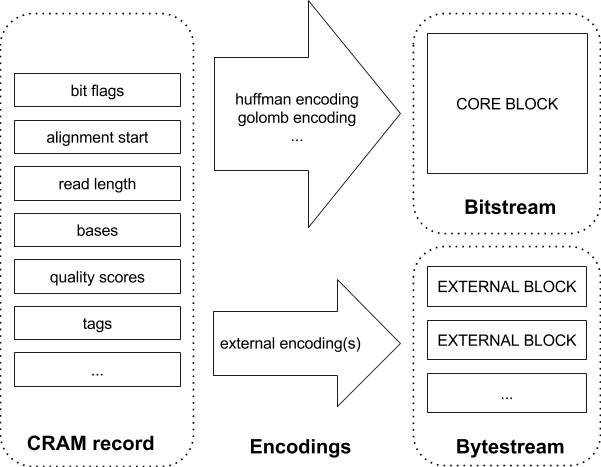
\includegraphics[width=451pt, height=350pt, keepaspectratio=true]{img/CRAMFileFormat2-1-fig007.png}
%%\caption{This should be the caption for \texttt{img/CRAMFileFormat2-1-fig007.png}.}
%%\end{figure}

Pic.3 Relationship between core data block and external data blocks.

The picture shows how a CRAM record (on the left) is partially written to core 
data block while the other fields are stored in two external data blocks. The specific 
encodings are presented only for demonstration purposes, the main point here is 
to distinguish between bit encodings whose output is always stored in core data 
block and the external encoding which simply stored the bytes into external data 
blocks.

\section{\textbf{End of file marker}}

A special container is used to mark the end of a file or stream. It is required in version 3 or later. The idea is to provide an easy and a quick way to detect that a CRAM file or stream is complete. The marker is basically an empty container with ref seq id set to -1 (unaligned) and alignment 
start set to 4542278.

Here is a complete content of the EOF container explained in detail:

\begin{tabular}{|l|l|>{\raggedright}p{150pt}|>{\raggedright}p{180pt}|}
\hline
\textbf{hex bytes} & \textbf{data type} & \textbf{decimal value} & \textbf{field 
name}\tabularnewline
\hline
\multicolumn{4}{|l|}{\textit{Container header}}\tabularnewline
\hline
0f 00 00 00 & integer & 15 & size of blocks data\tabularnewline
\hline
ff ff ff ff 0f & itf8 & -1 & ref seq id\tabularnewline
\hline
e0 45 4f 46 & itf8 & 4542278 & alignment start\tabularnewline
\hline
00 & itf8 & 0 & alignment span\tabularnewline
\hline
00 & itf8 & 0 & number of records\tabularnewline
\hline
00 & itf8 & 0 & global record counter\tabularnewline
\hline
00 & itf8 & 0 & bases\tabularnewline
\hline
01 & itf8 & 1 & block count\tabularnewline
\hline
00 & array & 0 & landmarks\tabularnewline
\hline
05 bd d9 4f & integer & 1339669765 & container header CRC32\tabularnewline
\hline
\multicolumn{4}{|l|}{\textit{Compression header block}}\tabularnewline
\hline
00 & byte & 0 (RAW) & compression method\tabularnewline
\hline
01 & byte & 1 (COMPRESSION\_HEADER) & block content type\tabularnewline
\hline
00 & itf8 & 0 & block content id\tabularnewline
\hline
06 & itf8 & 6 & compressed size\tabularnewline
\hline
06 & itf8 & 6 & uncompressed size\tabularnewline
\hline
\multicolumn{4}{|l|}{\textit{Compression header}}\tabularnewline
\hline
01 & itf8 & 1 & preservation map byte size\tabularnewline
\hline
00 & itf8 & 0 & preservation map size\tabularnewline
\hline
01 & itf8 & 1 & encoding map byte size\tabularnewline
\hline
00 & itf8 & 0 & encoding map size\tabularnewline
\hline
01 & itf8 & 1 & tag encoding byte size\tabularnewline
\hline
00 & itf8 & 0 & tag encoding map size\tabularnewline
\hline
ee 63 01 4b & integer & 1258382318 & block CRC32\tabularnewline
\hline
\end{tabular}

When compiled together the EOF marker is 38 bytes long and in hex representation 
is:

0f 00 00 00 ff ff ff ff 0f e0 45 4f 46 00 00 00 00 01 00 05 bd d9 4f 00 01 00 06 06 01 00 01 00 01 00 ee 63 01 4b

\section{\textbf{Record structure}}
\label{sec:record}

CRAM record is based on the SAM record but has additional features allowing for 
more efficient data storage.  In contrast to BAM record CRAM record uses bits as 
well as bytes for data storage. This way, for example, various coding techniques 
which output variable length binary codes can be used directly in CRAM. On the 
other hand, data series that do not require binary coding can be stored separately 
in external blocks with some other compression applied to them independently.

As CRAM data series may be interleaved within the same blocks\footnote{Interleaving can sometimes provide better compression, however it also adds dependency between types of data meaning it is not possible to selectively decode one data series if it co-locates with another data series in the same block.} understanding the order in which CRAM data series must be decoded is vital.

The overall flowchart is below, with more detailed description in the subsequent sections.

\algnewcommand\algorithmicto{\text{ \textbf{to} }}

\subsection{\textbf{CRAM record}}

Both mapped and unmapped reads start with the following fields. Please note that 
the data series type refers to the logical data type and the data series name corresponds 
to the data series encoding map.

\begin{tabular}{|>{\raggedright}p{70pt}|>{\raggedright}p{75pt}|>{\raggedright}p{90pt}|>{\raggedright}p{171pt}|}
\hline
\textbf{Data series type} & \textbf{Data series name} & \textbf{Field} & \textbf{Description}\tabularnewline
\hline
int & BF & BAM bit flags & see BAM bit flags below\tabularnewline
\hline
int & CF & CRAM bit flags & see CRAM bit flags below\tabularnewline
\hline
- & - & Positional data & See section \ref{subsec:positions}\tabularnewline
\hline
- & - & Read names & See section \ref{subsec:names}\tabularnewline
\hline
- & - & Mate records & See section \ref{subsec:mate}\tabularnewline
\hline
- & - & Auxiliary tags & See section \ref{subsec:tags}\tabularnewline
\hline
- & - & Sequences & See sections \ref{subsec:mapped} and \ref{subsec:unmapped}\tabularnewline
\hline
\end{tabular}

\subsubsection*{\textbf{BAM bit flags (BF data series)}}

The following flags are duplicated from the SAM and BAM specification, with identical meaning.
Note however some of these flags can be derived during decode, so may be omitted in the CRAM file and the bits computed based on both reads of a pair-end library residing within the same slice.

\begin{threeparttable}[t]
\begin{tabular}{|>{\raggedright}p{144pt}|>{\raggedright}p{144pt}|>{\raggedright}p{144pt}|}
\hline
\textbf{Bit flag} & \textbf{Comment} & \textbf{Description}\tabularnewline
\hline
0x1 &  & template having multiple segments in sequencing\tabularnewline
\hline
0x2 &  & each segment properly aligned according to the aligner\tabularnewline
\hline
0x4 &  & segment unmapped\tnote{a}\tabularnewline
\hline
0x8 & calculated\tnote{b}\ \ or stored in the mate's info & next segment in template unmapped\tabularnewline
\hline
0x10 &  & SEQ being reverse complemented\tabularnewline
\hline
0x20 & calculated\tnote{b}\ \ or stored in the mate's info & SEQ of the next segment in the
template being reversed\tabularnewline
\hline
0x40 &  & the first segment in the template\tnote{c}\tabularnewline
\hline
0x80 &  & the last segment in the template\tnote{c}\tabularnewline
\hline
0x100 &  & secondary alignment\tabularnewline
\hline
0x200 &  & not passing quality controls\tabularnewline
\hline
0x400 &  & PCT or optical duplicate\tabularnewline
\hline
0x800 &  & Supplementary alignment\tabularnewline
\hline
\end{tabular}
\begin{tablenotes}
\item[a] Bit 0x4 is the only reliable place to tell whether the read is unmapped.  If 0x4 is set, no assumptions may be made about bits 0x2, 0x100 and 0x800.
\item[b] For segments within the same slice.
\item[c] Bits 0x40 and 0x80 reflect the read ordering within each template inherent in the sequencing technology used, which may be independent from the actual mapping orientation.
If 0x40 and 0x80 are both set, the read is part of a linear template (one where the template sequence is expected to be in a linear order), but it is neither the first nor the last read.
If both 0x40 and 0x80 are unset, the index of the read in the template is unknown.
This may happen for a non-linear template (such as one constructed by stitching together other templates) or when this information is lost during data processing.
\end{tablenotes}
\end{threeparttable}

\subsubsection*{\textbf{CRAM bit flags (CF data series)}}

The CRAM bit flags (also known as compression bit flags) expressed as an integer represent the CF data series. 
The following compression flags are defined for each CRAM read record:

\begin{tabular}{|>{\raggedright}p{39pt}|>{\raggedright}p{150pt}|>{\raggedright}p{242pt}|}
\hline
\textbf{Bit flag} & \textbf{Name} & \textbf{Description}\tabularnewline
\hline
0x1 & quality scores stored as array & quality scores can be stored as read features
or as an array similar to read bases.\tabularnewline
\hline
0x2 & detached & mate information is stored verbatim (e.g. because the pair spans multiple slices or the fields differ to the CRAM computed method)\tabularnewline
\hline
0x4 & has mate downstream & tells if the next segment should be expected further
in the stream\tabularnewline
\hline
0x8 & decode sequence as ``*'' & informs the decoder that the sequence
is unknown and that any encoded reference differences are present only to
recreate the CIGAR string.\tabularnewline
\hline
\end{tabular}


The following pseudocode describes the general process of decoding an entire CRAM record.
The sequence data itself is in one of two encoding formats depending on whether the record is aligned (mapped).

\subsubsection*{\textbf{Decode pseudocode}}
\newlength{\maxwidth}
\newcommand{\algalign}[2] % #1 = text to left, #2 = text to right
{\makebox[\maxwidth][l]{$#1{}$}${}#2$}

\begin{algorithmic}[1]
\Procedure{DecodeRecord}{}
\settowidth{\maxwidth}{CRAM\_flags\quad}
\State \algalign{BAM\_flags}{\gets}  \Call{ReadItem}{BF, Integer}
\State \algalign{CRAM\_flags}{\gets} \Call{ReadItem}{CF, Integer}
\State \Call{DecodePositions}{}\Comment{See section \ref{subsec:positions}}
\State \Call{DecodeNames}{}\Comment{See section \ref{subsec:names}}
\State \Call{DecodeMateData}{}\Comment{See section \ref{subsec:mate}}
\State \Call{DecodeTagData}{}\Comment{See section \ref{subsec:tags}}
\Statex

\If{$(BF$ AND $4) \ne 0$}\Comment{Unmapped flag}
  \State \Call{DecodeMappedRead}{}\Comment{See section \ref{subsec:mapped}}
\Else
  \State \Call{DecodeUnmappedRead}{}\Comment{See section \ref{subsec:unmapped}}
\EndIf
\EndProcedure
\end{algorithmic}

\subsection{\textbf{CRAM positional data}}
\label{subsec:positions}

Following the bit-wise BAM and CRAM flags, CRAM encodes positional related data including reference, alignment positions and length, and read-group.
Positional data is stored for both mapped and unmapped sequences, as unmapped data may still be ``placed'' at a specific location in the genome (without being aligned).
Typically this is done to keep a sequence pair (paired-end or mate-pair sequencing libraries) together when one of the pair aligns and the other does not.

The AP data series is delta encoded for reads mapped to a position-sorted slice containing data from a single reference, and as a normal integer value in all other cases.

\begin{tabular}{|>{\raggedright}p{70pt}|>{\raggedright}p{75pt}|>{\raggedright}p{90pt}|>{\raggedright}p{171pt}|}
\hline
\textbf{Data series type} & \textbf{Data series name} & \textbf{Field} & \textbf{Description}\tabularnewline
\hline
int & RI & ref id & reference sequence id (only present in multiref slices)\tabularnewline
\hline
int & RL & read length & the length of the read\tabularnewline
\hline
int & AP & alignment start & the alignment start position\tabularnewline
\hline
int & RG & read group & the read group identifier expressed as the N\textsuperscript{th} record in the header, starting from 0 with -1 for no group\tabularnewline
\hline
\end{tabular}

\vskip 20pt
\begin{algorithmic}[1]
\Procedure{DecodePositions}{}
\If{$slice\_header.reference\_sequence\_id = -2$}
  \State $reference\_id\gets$ \Call{ReadItem}{RI, Integer}
\Else
  \State $reference\_id\gets slice\_header.reference\_sequence\_id$
\EndIf
\State $read\_length \gets$ \Call{ReadItem}{RL, Integer}
\If{$container\_pmap.AP\_delta \ne 0$}
    \State Initialise $last\_position$ to 0 if first record in slice
    \State $alignment\_position \gets$ \Call{ReadItem}{AP, Integer} + $last\_position$
    \State $last\_position \gets alignment\_position$
\Else
    \State $alignment\_position \gets$ \Call{ReadItem}{AP, Integer}
\EndIf
\State $read\_group \gets$ \Call{ReadItem}{RG, Integer}
\EndProcedure
\end{algorithmic}

\subsection{Read names (RN data series)}
\label{subsec:names}

Read names can be preserved in the CRAM format, but this is optional and is governed by the \texttt{RN} preservation map key in the container compression header. See section \ref{subsec:compression-header}.
When read names are not preserved the CRAM decoder should generate names, typically based on the file name and a numeric ID of the read using the record counter field of the slice header block.
Note read names may still be preserved even when the \texttt{RN} compression header key indicates otherwise, such as where a read is part of a read-pair and the pair spans multiple slices.
In this situation the record will be marked as detached (see the CF data series) and the mate data below (section \ref{subsec:mate}) will contain the read name.

\begin{tabular}{|>{\raggedright}p{70pt}|>{\raggedright}p{75pt}|>{\raggedright}p{90pt}|>{\raggedright}p{171pt}|}
\hline
\textbf{Data series type} & \textbf{Data series name} & \textbf{Field} & \textbf{Description}\tabularnewline
\hline
byte[] & RN & read names & read names\tabularnewline
\hline
\end{tabular}

\vskip 20pt
\begin{algorithmic}[1]
\Procedure{DecodeNames}{}
\If{$container\_pmap.read\_names\_included = 1$}
  \State $read\_name \gets$ \Call{ReadItem}{RN, Byte[]}
\Else
  \State $read\_name \gets$ \Call{GenerateName}{}
\EndIf
\Statex
\EndProcedure
\end{algorithmic}

\subsection{\textbf{Mate record}}
\label{subsec:mate}

There are two ways in which mate information can be preserved in CRAM: number of records downstream (distance, within this slice) to the next fragment in the template and a special mate record if the next fragment is not in the current slice.
In the latter case the record is labelled as ``detached'', see the CF data series.

For mates within the slice only the distance is captured, and only for the first record.  The mate has neither detached nor downstream flags set in the CF data series.

\begin{tabular}{|>{\raggedright}p{68pt}|>{\raggedright}p{115pt}|>{\raggedright}p{228pt}|}
\hline
\textbf{Data series type} & \textbf{Data series name} & \textbf{Description}\tabularnewline
\hline
int & NF & the number of records to the next fragment\tabularnewline
\hline
\end{tabular}

In the above case, the NS (mate reference name), NP (mate position) and TS (template size) fields for both records should be derived once the mate has also been decoded.
Mate reference name and position are obvious and simply copied from the mate.
The template size is computed using the method described in the SAM specification; the inclusive distance from the leftmost to rightmost mapped bases with the sign being positive for the leftmost record and negative for the rightmost record.

If the next fragment is not found within this slice then the following structure is included into the CRAM record.
Note there are cases where read-pairs within the same slice may be marked as detached and use this structure, such as to store mate-pair information that does not match the algorithm used by CRAM for computing the mate data on-the-fly.

\begin{tabular}{|>{\raggedright}p{66pt}|>{\raggedright}p{117pt}|>{\raggedright}p{228pt}|}
\hline
\textbf{Data series type} & \textbf{Data series name} & \textbf{Description}\tabularnewline
\hline
int & MF & next mate bit flags, see table below\tabularnewline
\hline
byte[ ] & RN & the read name (if and only if not known already)\tabularnewline
\hline
int & NS & mate reference sequence identifier \tabularnewline
\hline
int & NP & mate alignment start position \tabularnewline
\hline
int & TS & the size of the template (insert size)\tabularnewline
\hline
\end{tabular}

\subsubsection*{Next mate bit flags (MF data series)}

The next mate bit flags expressed as an integer represent the MF data series.
These represent the missing bits we excluded from the BF data series (when compared to the full SAM/BAM flags).
The following bit flags are defined:

\begin{tabular}{|>{\raggedright}p{47pt}|>{\raggedright}p{134pt}|>{\raggedright}p{250pt}|}
\hline
\textbf{Bit flag} & \textbf{Name} & \textbf{Description}\tabularnewline
\hline
0x1 & mate negative strand bit & the bit is set if the mate is on the negative
strand\tabularnewline
\hline
0x2 & mate mapped bit & the bit is set if the mate is mapped\tabularnewline
\hline
\end{tabular}


\subsubsection*{\textbf{Decode mate pseudocode}}

In the following pseudocode we are assuming the current record is $this$ and its mate is $next\_frag$.

\begin{algorithmic}[1]
\Procedure{DecodeMateData}{}
\If{$CF$ AND $2$}\Comment{Detached from mate}
  \State $mate\_flags\gets $ \Call{ReadItem}{MF,Integer}
  \If{$mate\_flags$ AND 1}
    \State $bam\_flags\gets bam\_flags$\ OR\ 0x20\Comment{Mate is reverse-complemented}
  \EndIf
  \If{$mate\_flags$ AND 2}
    \State $bam\_flags\gets bam\_flags$\ OR\ 0x08\Comment{Mate is unmapped}
  \EndIf
  \If{$container\_pmap.read\_names\_included \ne 1$}
    \State $read\_name \gets$ \Call{ReadItem}{RN, Byte[]}
  \EndIf
\settowidth{\maxwidth}{mate\_position\ }
\State \algalign{mate\_ref\_id}{\gets}  \Call{ReadItem}{NS, Integer}
\State \algalign{mate\_position}{\gets} \Call{ReadItem}{NP, Integer}
\State \algalign{template\_size}{\gets} \Call{ReadItem}{TS, Integer}
\ElsIf{$CF$ AND $4$}\Comment{Mate is downstream}
  \If{$next\_frag.bam\_flags$ AND 0x10}
    \State $this.bam\_flags \gets this.bam\_flags$\ OR\ 0x20\Comment{next segment reverse complemented}
  \EndIf
  \If{$next\_frag.bam\_flags$ AND 0x04}
    \State $this.bam\_flags \gets this.bam\_flags$\ OR\ 0x08\Comment{next segment unmapped}
  \EndIf
  \State $next\_frag\gets$ \Call{ReadItem}{NF,Integer}
  \State Resolve $mate\_ref\_id$ for $this$ record and $this+next\_frag$ once both have been decoded
  \State Resolve $mate\_position$ for $this$ record and $this+next\_frag$ once both have been decoded
  \State Find leftmost and rightmost mapped coordinate in records $this$ and $this+next\_frag$.
  \State For leftmost of $this$ and $this+next\_frag$ record: $template\_size\gets rightmost-leftmost+1$
  \State For rightmost of $this$ and $this+next\_frag$ record: $template\_size\gets -(rightmost-leftmost+1)$
\EndIf
\EndProcedure
\end{algorithmic}

Note as with the SAM specification a template may be permitted to have more than two alignment records.
In this case the ``mate'' for each record is considered to be the next record, with the mate for the last record being the first to form a circular list.
The above algorithm is a simplification that does not deal with this scenario.
The full method needs to observe when record $this+NF$ is also labelled as having an additional mate downstream.
One recommended approach is to resolve the mate information in a second pass, once the entire slice has been decoded.
The final segment in the mate chain needs to set $bam\_flags$ fields 0x20 and 0x08 accordingly based on the first segment.
This is also not listed in the above algorithm, for brevity.

\subsection{Auxiliary tags}
\label{subsec:tags}

Tags are encoded using a tag line (TL data series) integer into the tag dictionary (TD field in the compression header preservation map, see section \ref{subsec:compression-header}).
See section \ref{subsubsec:tags} for a more detailed description of this process.

\begin{tabular}{|>{\raggedright}p{70pt}|>{\raggedright}p{75pt}|>{\raggedright}p{90pt}|>{\raggedright}p{200pt}|}
\hline
\textbf{Data series type} & \textbf{Data series name} & \textbf{Field} & \textbf{Description}\tabularnewline
\hline
int & TL & tag line & an index into the tag dictionary (TD)\tabularnewline
\hline
* & ??? & tag name/type & 3 character key (2 tag identifier and 1 tag type), as specified by the tag dictionary\tabularnewline
\hline
\end{tabular}

\vskip 20pt
\begin{algorithmic}[1]
\Procedure{DecodeTagData}{}
\State $tag\_line\gets$ \Call{ReadItem}{TL,Integer}
\ForAll {$ele \in container\_pmap.tag\_dict(tag\_line)$}
  \State $name\gets$ first two characters of $ele$
  \State $tag(type)\gets$ last character of $ele$
  \State $tag(name)\gets$ \Call{ReadItem}{$ele$, Byte[]}
\EndFor
\EndProcedure
\end{algorithmic}

In the above procedure, $name$ is a two letter tag name and $type$ is one of the permitted types documented in the SAM/BAM specification.
Type is \texttt{c} (signed 8-bit integer), \texttt{C} (unsigned 8-bit integer), \texttt{s} (signed 16-bit integer), \texttt{S} (unsigned 16-bit integer), \texttt{i} (signed 32-bit integer), \texttt{I} (unsigned 32-bit integer), \texttt{f} (32-bit float), \texttt{Z} (nul-terminated string), \texttt{H} (nul-terminated string of hex digits) and \texttt{B} (binary data in array format with the first byte being one of c,C,s,S,i,I,f using the meaning above, a 32-bit integer for the number of array elements, followed by array data encoded using the specified format).  All integers are little endian encoded.

For example a SAM tag \texttt{MQ:i} has name \texttt{MQ} and type \texttt{i} and will be decoded using one of MQc, MQC, MQs, MQS, MQi and MQI data series depending on size and sign of the integer value.

\subsection{\textbf{Mapped reads}}
\label{subsec:mapped}

\subsubsection*{\textbf{Read feature records}}
\label{subsec:features}

Read features are used to store read details that are expressed using read coordinates 
(e.g. base differences respective to the reference sequence). The read feature 
records start with the number of read features followed by the read features themselves.
Finally the single mapping quality and per-base quality scores are stored.

\begin{threeparttable}[t]
\begin{tabular}{|>{\raggedright}p{88pt}|>{\raggedright}p{83pt}|>{\raggedright}p{85pt}|>{\raggedright}p{180pt}|}
\hline
\textbf{Data series type} & \textbf{Data series name} & \textbf{Field} & \textbf{Description}\tabularnewline
\hline
int & FN & number of read features & the number of read features\tabularnewline
\hline
int & FP & in-read-position\tnote{a} & position of the read feature\tabularnewline 
\hline
byte & FC & read feature code\tnote{a} & See feature codes below\tabularnewline
\hline
* & * & read feature data\tnote{a} & See feature codes below\tabularnewline
\hline
int & MQ & mapping qualities & mapping quality score\tabularnewline
\hline
byte[read length] & QS & quality scores & the base qualities, if preserved\tabularnewline
\hline
\end{tabular}
\begin{tablenotes}
\item[a] Repeated FN times, once for each read feature.
\end{tablenotes}
\end{threeparttable}

\subsubsection*{Read feature codes}

Each feature code has its own associated data series containing further information specific to that feature.
The following codes are used to distinguish variations in read coordinates:

\begin{tabular}{|>{\raggedright}p{91pt}|>{\raggedright}p{45pt}|>{\raggedright}p{72pt}|>{\raggedright}p{66pt}|>{\raggedright}p{132pt}|}
\hline
\textbf{Feature code} & \textbf{Id} & \textbf{Data series type} & \textbf{Data 
series name} & \textbf{Description}\tabularnewline
\hline
Bases & b (0x62) & byte[ ] & BB & a stretch of bases\tabularnewline
\hline
Scores & q (0x71) & byte[ ] & QQ & a stretch of scores\tabularnewline
\hline
% Neither C nor Java implementations generator nor can decode the 'A'
% feature code, but if they did they'd be BB/QQ and not BA/QS.  Best
% to omit it from published spec for now?
%
% Bases and scores & A (0x41) & byte[ ],byte[ ] & BB,QQ & A a stretch of bases and
% quality scores score\tabularnewline
% \hline
Read base & B (0x42) & byte,byte & BA,QS & A base and associated quality score\tabularnewline
\hline
Substitution & X (0x58) & byte & BS & base substitution codes, SAM operators X, 
M and =\tabularnewline
\hline
Insertion & I (0x49) & byte[ ] & IN & inserted bases, SAM operator I\tabularnewline
\hline
Deletion & D (0x44) & int & DL & number of deleted bases, SAM operator D\tabularnewline
\hline
Insert base & i (0x69) & byte & BA & single inserted base, SAM operator I\tabularnewline
\hline
Quality score & Q (0x51) & byte & QS & single quality score\tabularnewline
\hline
Reference skip & N (0x4E) & int & RS & number of skipped bases, SAM operator N\tabularnewline
\hline
Soft clip & S (0x53) & byte[ ] & SC & soft clipped bases, SAM operator S\tabularnewline
\hline
Padding & P (0x50) & int & PD & number of padded bases, SAM operator P\tabularnewline
\hline
Hard clip & H (0x48) & int & HC & number of hard clipped bases, SAM operator H\tabularnewline
\hline
\end{tabular}

\subsubsection*{Base substitution codes (BS data series)}

A base substitution is defined as a change from one nucleotide base (reference 
base) to another (read base) including N as an unknown or missing base. There are 
5 possible bases ACGTN, 4 possible substitutions for each base and 20 substitutions 
in total. Substitutions for the same reference base are assigned integer codes 
from 0 to 3 inclusive. To restore a base one would need to know its substitution 
code and the reference base. 

A base substitution matrix assigns integer codes to all possible substitutions. 

Substitution matrix is written as follows. Substitutions for a given reference 
base are sorted by their frequencies in descending order then assigned numbers 
from 0 to 3. Same-frequency ties are broken using alphabetical order. For example, 
let us assume the following substitution frequencies for base A: 

AC: 15\%

AG: 25\%

AT: 55\%

AN: 5\%

Then the substitution codes are: 

AC: 2

AG: 1

AT: 0

AN: 3

and they are written as a single byte, 10 01 00 11 = 147 decimal or 0x93 in this 
case. The whole substitution matrix is written as 5 bytes, one for each reference 
base in the alphabetical order: A, C, G, T and N.

Note: the last two bits of each substitution code are redundant but still required 
to simplify the reading. 

\subsubsection*{Decode mapped read pseudocode}

\begin{algorithmic}[1]
\Procedure{DecodeMappedRead}{}
  \State $feature\_number\gets$ \Call{ReadItem}{FN, Integer} 
  \For{$i\gets 1 \algorithmicto feature\_number$}
    \State \Call{DecodeFeature}{}
  \EndFor
  \State $mapping\_quality\gets$ \Call{ReadItem}{MQ, Integer} 
  \If{$container\_pmap.preserve\_quality\_scores$}
    \For{$i\gets 1 \algorithmicto read\_length$}
      \State $quality\_score\gets$ \Call{ReadItem}{QS, Integer} 
    \EndFor
  \EndIf
\EndProcedure
\Statex
\Procedure{DecodeFeature}{}
    \settowidth{\maxwidth}{feature\_position\ }
    \State \algalign{feature\_code}{\gets}       \Call{ReadItem}{FC, Integer} 
    \State \algalign{feature\_position}{\gets}   \Call{ReadItem}{FP, Integer} 
    \settowidth{\maxwidth}{substitution\_code\ }
    \If{$feature\_code = $`B'}
      \State \algalign{base}{\gets}              \Call{ReadItem}{BA, Byte}
      \State \algalign{quality\_score}{\gets}    \Call{ReadItem}{QS, Byte}
    \ElsIf{$feature\_code = $`X'}
      \State \algalign{substitution\_code}{\gets} \Call{ReadItem}{BS, Byte}
    \ElsIf{$feature\_code = $`I'}
      \State \algalign{inserted\_bases}{\gets}   \Call{ReadItem}{IN, Byte[]}
    \ElsIf{$feature\_code = $`S'}
      \State \algalign{softclip\_bases}{\gets}   \Call{ReadItem}{SC, Byte[]}
    \ElsIf{$feature\_code = $`H'}
      \State \algalign{hardclip\_length}{\gets}  \Call{ReadItem}{HC, Integer}
    \ElsIf{$feature\_code = $`P'}
      \State \algalign{pad\_length}{\gets}       \Call{ReadItem}{PD, Integer}
    \ElsIf{$feature\_code = $`D'}
      \State \algalign{deletion\_length}{\gets}  \Call{ReadItem}{DL, Integer}
    \ElsIf{$feature\_code = $`N'}
      \State \algalign{ref\_skip\_length}{\gets} \Call{ReadItem}{RS, Integer}
    \ElsIf{$feature\_code = $`i'}
      \State \algalign{base}{\gets}              \Call{ReadItem}{BA, Byte}
    \ElsIf{$feature\_code = $`b'}
      \State \algalign{bases}{\gets}             \Call{ReadItem}{BB, Byte[]}
    \ElsIf{$feature\_code = $`q'}
      \State \algalign{quality\_scores}{\gets}   \Call{ReadItem}{QQ, Byte[]}
    \ElsIf{$feature\_code = $`Q'}
      \State \algalign{quality\_score}{\gets}    \Call{ReadItem}{QS, Byte}
    \EndIf
\EndProcedure
\end{algorithmic}

\subsection{\textbf{Unmapped reads}}
\label{subsec:unmapped}

The CRAM record structure for unmapped reads has the following additional fields:

\begin{tabular}{|>{\raggedright}p{88pt}|>{\raggedright}p{83pt}|>{\raggedright}p{85pt}|>{\raggedright}p{180pt}|}
\hline
\textbf{Data series type} & \textbf{Data series name} & \textbf{Field} & \textbf{Description}\tabularnewline
\hline
byte[read length] & BA & bases & the read bases\tabularnewline
\hline
byte[read length] & QS & quality scores & the base qualities, if preserved\tabularnewline
\hline
\end{tabular}

\vskip20pt
\begin{algorithmic}[1]
\Procedure{DecodeUnmappedRead}{}
  \For{$i\gets 1 \algorithmicto read\_length$}
    \State $base\gets$ \Call{ReadItem}{BA, Byte}
  \EndFor
  \If{$container\_pmap.preserve\_quality\_scores$}
    \For{$i\gets 1 \algorithmicto read\_length$}
      \State $quality\_score\gets$ \Call{ReadItem}{QS, Byte}
    \EndFor
  \EndIf
\EndProcedure
\end{algorithmic}

\section{\textbf{Reference sequences}}

CRAM format is natively based upon usage of reference sequences even though in 
some cases they are not required. In contrast to BAM format CRAM format has strict 
rules about reference sequences. 

\begin{enumerate}
\item M5 (sequence MD5 checksum) field of @SQ sequence record in the BAM header is 
required and UR (URI for the sequence fasta optionally gzipped file) field is strongly 
advised. The rule for calculating MD5 is to remove any non-base symbols (like \textbackslash{}n, 
sequence name or length and spaces) and upper case the rest. Here are some examples: 

\texttt{> samtools faidx human\_g1k\_v37.fasta 1 \textbar{} grep -v '\textasciicircum{}>' \textbar{} tr -d '\textbackslash{}n' \textbar{} tr a-z A-Z \textbar{} md5sum -\\
1b22b98cdeb4a9304cb5d48026a85128  -}

\texttt{> samtools faidx human\_g1k\_v37.fasta 1:10-20 \textbar{}grep -v '\textasciicircum{}\texttt{>}' \textbar{}tr -d '\textbackslash{}n' \textbar{}tr a-z A-Z \textbar{}md5sum -\\
0f2a4865e3952676ffad2c3671f14057  -}

Please note that the latter calculates the checksum for 11 bases from position 
10 (inclusive) to 20 (inclusive) and the bases are counted 1-based, so the first 
base position is 1. 

\item All CRAM reader implementations are expected to check for reference MD5 checksums 
and report any missing or mismatching entries. Consequently, all writer implementations 
are expected to ensure that all checksums are injected or checked during compression 
time. 

\item In some cases reads may be mapped beyond the reference sequence. All out of 
range reference bases are all assumed to be `N'. 

\item MD5 checksum bytes in slice header should be ignored for unmapped or multiref 
slices. 
\end{enumerate}

\section{\textbf{Indexing}}

\subsubsection*{General notes}

Please note that CRAM indexing is external to the file format itself and may change 
independently of the file format specification in the future. For example, a new 
type of index files may appear. 

Individual records are not indexed in CRAM files, slices should be used instead 
as a unit of random access. Another important difference between CRAM and BAM indexing 
is that CRAM container header and compression header block (first block in container) 
must always be read before decoding a slice. Therefore two read operations are 
required for random access in CRAM.

Indexing a CRAM file is deemed to be a lightweight operation because it does not 
require any CRAM records to be read. All indexing information can be obtained from 
container headers, namely sequence id, alignment start and span, container start 
byte offset and slice byte offset inside the container. 

\subsubsection*{CRAM index}

A CRAM index is a gzipped tab delimited file containing the following columns:

\begin{enumerate}
\item Sequence id

\item Alignment start

\item Alignment span

\item Container start byte offset in the file

\item Slice start byte offset in the container data (`blocks')

\item Slice bytes
\end{enumerate}

Each line represents a slice in the CRAM file. Please note that all slices must 
be listed in index file.

\subsubsection*{BAM index}

BAM indexes are supported by using 4-byte integer pointers called landmarks that 
are stored in container header. BAM index pointer is a 64-bit value with 48 bits 
reserved for the BAM block start position and 16 bits reserved for the in-block 
offset. When used to index CRAM files, the first 48 bits are used to store the 
CRAM container start position and the last 16 bits are used to store the index 
of the landmark in the landmark array stored in  container header. The landmark 
index can be used to access the appropriate slice. 

The above indexing scheme treats CRAM slices as individual records in BAM file. 
This allows to apply BAM indexing to CRAM files, however it introduces some overhead 
in seeking specific alignment start because all preceding records in the slice 
must be read and discarded.

\section{\textbf{Encodings}}

% FIXME: we have a mishash of coding, encoding and codec.  We should
% go through the entire document and be consistent.

\subsection{\textbf{Introduction}}

The basic idea for codings is to efficiently represent some values in binary format. 
This can be achieved in a number of ways that most frequently involve some knowledge 
about the nature of the values being encoded, for example, distribution statistics. 
The methods for choosing the best encoding and determining its parameters are very 
diverse and are not part of the CRAM format specification, which only describes 
how the information needed to decode the values should be stored.

Note two of the encodings (Golomb and Golomb-Rice) are listed as deprecated.
These are still formally part of the CRAM specification, but have not been used by the primary implementations and may not be well supported.
Therefore their use is permitted, but not recommended.

\subsubsection*{Offset}

Many of the codings listed below encode positive integer numbers. An integer offset 
value is used to allow any integer numbers and not just positive ones to be encoded. 
It can also be used for monotonically decreasing distributions with the maximum 
not equal to zero. For example, given offset is 10 and the value to be encoded 
is 1, the actually encoded value would be offset+value=11. Then when decoding, 
the offset would be subtracted from the decoded value. 

\subsection{External: codec ID 1}

Can encode types \textit{Byte}, \textit{Integer}.

External coding is simply storage of data verbatim to an external block with a given ID.
If the type is \textit{Byte} the data is stored as-is, otherwise for \textit{Integer} type the data is stored in ITF8.

\subsubsection*{Parameters}

CRAM format defines the following parameters of external coding: 

\begin{tabular}{|>{\raggedright}p{100pt}|>{\raggedright}p{100pt}|>{\raggedright}p{230pt}|}
\hline
\textbf{Data type} & \textbf{Name} & \textbf{Comment}
\tabularnewline
\hline
itf8 & external id & id of an external block containing the byte stream\tabularnewline
\hline
\end{tabular}

\subsection{Huffman coding: codec ID 3}

Can encode types \textit{Byte}, \textit{Integer}.

Huffman coding replaces symbols (values to encode) by binary codewords, with common symbols having shorter codewords such that the total message of binary codewords is shorter than using uniform binary codeword lengths.
The general process consists of the following steps.

\begin{itemize}
\item Obtain symbol code lengths.
\begin{itemize}
\item If encoding:\\
- Compute symbol frequencies.\\
- Compute code lengths from frequencies.
\item If decoding:\\
- Read code lengths from codec parameters.
\end{itemize}

\item Compute canonical Huffman codewords from code lengths\footnote{\url{https://en.wikipedia.org/wiki/Canonical_Huffman_code}}.

\item Encode or decode bits as per the symbol to codeword table.
Codewords have the ``prefix property'' that no codeword is a prefix of another codeword, enabling unambiguous decode bit by bit.
\end{itemize}

The use of canonical Huffman codes means that we only need to store the code lengths and use the same algorithm in both encoder and decoder to generate the codewords.
This is achieved by ensuring our symbol alphabet has a natural sort order and codewords are assigned in numerical order.

\textbf{Important note: for alphabets with only one value, the codeword will be zero bits long.}
This makes the Huffman codec an efficient mechanism for specifying constant values.

\subsubsection*{Canonical code computation}

\begin{enumerate}
\item Sort the alphabet ascending using bit-lengths and then using numerical order 
of the values.

\item The first symbol in the list gets assigned a codeword which is the same length 
as the symbol's original codeword but all zeros. This will often be a single zero 
('0').

\item Each subsequent symbol is assigned the next binary number in sequence, ensuring
that following codes are always higher in value.

\item When you reach a longer codeword, then after incrementing, append zeros until 
the length of the new codeword is equal to the length of the old codeword.
\end{enumerate}

\subsubsection*{Examples}

\begin{tabular}{|>{\raggedright}p{105pt}|>{\raggedright}p{105pt}|>{\raggedright}p{105pt}|}
\hline
\textbf{Symbol} & \textbf{Code length} & \textbf{Codeword}\tabularnewline
\hline
A & 1 & 0\tabularnewline
\hline
B & 3 & 100\tabularnewline
C & 3 & 101\tabularnewline
D & 3 & 110\tabularnewline
\hline
E & 4 & 1110\tabularnewline
F & 4 & 1111\tabularnewline
\hline
\end{tabular}

\subsubsection*{Parameters}

\begin{tabular}{|>{\raggedright}p{100pt}|>{\raggedright}p{100pt}|>{\raggedright}p{230pt}|}
\hline
\textbf{Data type} & \textbf{Name} & \textbf{Comment}
\tabularnewline
\hline
itf8[ ] & alphabet & list of all encoded symbols (values)\tabularnewline
\hline
itf8[ ] & bit-lengths & array of bit-lengths for each symbol in the alphabet\tabularnewline
\hline
\end{tabular}

\subsection{Byte array coding}

Often there is a need to encode an array of bytes where the length is not predetermined.
For example the read identifiers differ per alignment record, possibly with different lengths, and this length must be stored somewhere.
There are two choices available: storing the length explicitly (BYTE\_ARRAY\_LEN) or continuing to read bytes until a termination value is seen (BYTE\_ARRAY\_STOP).

Note in contrast to this, quality values are known to be the same length as the sequence which is an already known quantity, so this does not need to be encoded using the byte array codecs.

\subsubsection*{BYTE\_ARRAY\_LEN: codec ID 4}

Can encode types \textit{Byte[]}.

Byte arrays are captured length-first, meaning that the length of every array element is written using an additional encoding.
For example this could be a HUFFMAN encoding or another EXTERNAL block.
The length is decoded first followed by the data, followed by the next length and data, and so on.

This encoding can therefore be considered as a nested encoding, with each pair of nested encodings containing their own set of parameters.
The byte stream for parameters of the BYTE\_ARRAY\_LEN encoding is therefore the concatenation of the length and value encoding parameters as described in section~\ref{subsec:writing-bytes}.

The parameter for BYTE\_ARRAY\_LEN are listed below:

\begin{tabular}{|>{\raggedright}p{100pt}|>{\raggedright}p{100pt}|>{\raggedright}p{230pt}|}
\hline
\textbf{Data type} & \textbf{Name} & \textbf{Comment}
\tabularnewline
\hline
encoding\texttt{<}int\texttt{>} & lengths encoding & an encoding describing how 
the arrays lengths are captured\tabularnewline
\hline
encoding\texttt{<}byte\texttt{>} & values encoding & an encoding describing how 
the values are captured\tabularnewline
\hline
\end{tabular}

For example, the bytes specifying a BYTE\_ARRAY\_LEN encoding, including the codec and parameters, for a 16-bit X0 auxiliary tag (``X0C'') may use HUFFMAN encoding to specify the length (always 2 bytes) and an EXTERNAL encoding to store the value to an external block with ID 200.

\begin{tabular}{lll}
\hline
\textbf{Bytes} & & \textbf{Meaning}\\
\hline
\texttt{0x04}         & & BYTE\_ARRAY\_LEN codec ID                                    \\
\texttt{0x0a}         & & 10 remaining bytes of BYTE\_ARRAY\_LEN parameters            \\
\\
\texttt{0x03}         & & HUFFMAN codec ID, for aux tag lengths                        \\
\texttt{0x04}         & & 4 more bytes of HUFFMAN parameters                           \\
\texttt{0x01}         & & Alphabet array size = 1                                      \\
\texttt{0x02}         & & alphabet symbol; (length = 2)                                \\
\texttt{0x01}         & & Codeword array size = 1                                      \\
\texttt{0x00}         & & Code length = 0 (zero bits needed as alphabet is size 1)     \\
\\
\texttt{0x01}         & & EXTERNAL codec ID, for aux tag values                        \\
\texttt{0x02}         & & 2 more bytes of EXTERNAL parameters                          \\
\texttt{0x80 0xc8}    & & ITF8 encoding for block ID 200                               \\
\hline
\end{tabular}



\subsubsection*{BYTE\_ARRAY\_STOP: codec ID 5}

Can encode types \textit{Byte[]}.

Byte arrays are captured as a sequence of bytes terminated by a special stop byte.
The data returned does not include the stop byte itself.
In contrast to BYTE\_ARRAY\_LEN the value is always encoded with EXTERNAL so the parameter is an external id instead of another encoding.

\begin{tabular}{|>{\raggedright}p{100pt}|>{\raggedright}p{100pt}|>{\raggedright}p{230pt}|}
\hline
\textbf{Data type} & \textbf{Name} & \textbf{Comment}
\tabularnewline
\hline
byte & stop byte & a special byte treated as a delimiter\tabularnewline
\hline
itf8 & external id & id of an external block containing the byte stream\tabularnewline
\hline
\end{tabular}

\subsection{Beta coding: codec ID 6}

Can encode types \textit{Integer}.

\subsubsection*{Definition}

Beta coding is a most common way to represent numbers in \emph{binary notation} and is sometimes referred to as binary coding.
The decoder reads the specified fixed number of bits (most significant first) and subtracts the offset value to get the decoded integer.

\subsubsection*{Parameters}

CRAM format defines the following parameters of beta coding: 

\begin{tabular}{|>{\raggedright}p{144pt}|>{\raggedright}p{144pt}|>{\raggedright}p{144pt}|}
\hline
\textbf{Data type} & \textbf{Name} & \textbf{Comment}\tabularnewline
\hline
itf8 & offset & offset is subtracted from each value during decode\tabularnewline
\hline
itf8 & length & the number of bits used\tabularnewline
\hline
\end{tabular}

\subsubsection*{Examples}

If we have integer values in the range 10 to 15 inclusive, the largest value would traditionally need 4 bits, but with an offset of -10 we can hold values 0 to 5, using a fixed size of 3 bits.
Using fixed Offset and Length coming from the beta parameters, we decode these values as:

\begin{tabular}{|>{\raggedright}p{105pt}|>{\raggedright}p{105pt}|>{\raggedright}p{105pt}|>{\raggedright}p{105pt}|}
\hline
Offset & Length & \textbf{Bits} & \textbf{Value}\tabularnewline
\hline
-10 & 3 & 000 & 10\tabularnewline
\hline
-10 & 3 & 001 & 11\tabularnewline
\hline
-10 & 3 & 010 & 12\tabularnewline
\hline
-10 & 3 & 011 & 13\tabularnewline
\hline
-10 & 3 & 100 & 14\tabularnewline
\hline
-10 & 3 & 101 & 15\tabularnewline
\hline
\end{tabular}

\subsection{Subexponential coding: codec ID 7}

Can encode types \textit{Integer}.

\subsubsection*{Definition}

Subexponential coding\footnote{Fast progressive lossless image compression, Paul G. Howard and Jeffrey Scott Vitter, 1994. \url{http://www.ittc.ku.edu/~jsv/Papers/HoV94.progressive_FELICS.pdf}} is parametrized by a non-negative integer $k$.
For values $n < 2^{k+1}$ subexponential coding produces codewords identical to Rice coding \footnote{\url{https://en.wikipedia.org/wiki/Golomb_coding\#Rice_coding}}.  For larger values it grows logarithmically with $n$.

\subsubsection*{Encoding}

\begin{enumerate}
\item Add $\mathit{offset}$ to $n$.

\item Determine $u$ and $b$ values from $n$
\begin{align*}
b =
\begin{cases}
  \ k                        & \text{ if $n < 2^k$} \\
  \ \lfloor log_{2}n \rfloor & \text{ if $n \ge 2^k$}
\end{cases}
&\
&u =
\begin{cases}
  \ 0     & \text{ if $n < 2^k$} \\
  \ b-k+1 & \text{ if $n \ge 2^k$}
\end{cases}
\end{align*}

\item Write $u$ in unary form; $u$ 1 bits followed by a single 0 bit.

\item Write the bottom $b$-bits of $n$ in binary form.
\end{enumerate}

\subsubsection*{Decoding}

\begin{enumerate}
\item Read $u$ in unary form, counting the number of leading 1s (prefix) in the codeword (discard the trailing 0 bit).

\item Determine $n$ via:
\begin{enumerate}
\item if $u = 0$ then read $n$ as a $k$-bit binary number.
\item if $u \ge 1$ then read $x$ as a $(u + k - 1)$-bit binary. Let $n = 2^{u+k-1} + x$.
\end{enumerate}

\item Subtract $\mathit{offset}$ from $n$.
\end{enumerate}

\subsubsection*{Examples}

\begin{tabular}{|>{\raggedright}p{105pt}|>{\raggedright}p{105pt}|>{\raggedright}p{105pt}|>{\raggedright}p{105pt}|}
\hline
\textbf{Number} & \textbf{Codeword, k=0} & \textbf{Codeword, k=1} & \textbf{Codeword, 
k=2}\tabularnewline
\hline
0 & 0 & 00 & 000\tabularnewline
\hline
1 & 10 & 01 & 001\tabularnewline
\hline
2 & 1100 & 100 & 010\tabularnewline
\hline
3 & 1101 & 101 & 011\tabularnewline
\hline
4 & 111000 & 11000 & 1000\tabularnewline
\hline
5 & 111001 & 11001 & 1001\tabularnewline
\hline
6 & 111010 & 11010 & 1010\tabularnewline
\hline
7 & 111011 & 11011 & 1011\tabularnewline
\hline
8 & 11110000 & 1110000 & 110000\tabularnewline
\hline
9 & 11110001 & 1110001 & 110001\tabularnewline
\hline
10 & 11110010 & 1110010 & 110010\tabularnewline
\hline
\end{tabular}

\subsubsection*{Parameters}

\begin{tabular}{|>{\raggedright}p{100pt}|>{\raggedright}p{100pt}|>{\raggedright}p{230pt}|}
\hline
\textbf{Data type} & \textbf{Name} & \textbf{Comment}
\tabularnewline
\hline
itf8 & offset & offset is subtracted from each value during decode\tabularnewline
\hline
itf8 & k & the order of the subexponential coding\tabularnewline
\hline
\end{tabular}

\subsection{Gamma coding: codec ID 9}

Can encode types \textit{Integer}.

\subsubsection*{Definition}

\emph{Elias gamma code} is a prefix encoding of positive integers. This is a combination 
of unary coding and beta coding. The first is used to capture the number of bits 
required for beta coding to capture the value. 

\subsubsection*{Encoding}

\begin{enumerate}
\item Write it in binary.

\item Subtract $1$ from the number of bits written in step 1 and prepend that many zeros.

\item An equivalent way to express the same process:

\item Separate the integer into the highest power of $2$ it contains ($2N$) and the remaining 
$N$ binary digits of the integer.

\item Encode $N$ in unary; that is, as $N$ zeroes followed by a one.

\item Append the remaining $N$ binary digits to this representation of $N$.
\end{enumerate}

\subsubsection*{Decoding}

\begin{enumerate}
\item Read and count 0s from the stream until you reach the first 1. Call this count 
of zeroes $N$.

\item Considering the one that was reached to be the first digit of the integer, with 
a value of $2N$, read the remaining $N$ digits of the integer.
\end{enumerate}

\subsubsection*{Examples}

\begin{tabular}{|>{\raggedright}p{76pt}|>{\raggedright}p{107pt}|}
\hline
\textbf{Value} & \textbf{Codeword}\tabularnewline
\hline
1 & 1\tabularnewline
\hline
2 & 010\tabularnewline
\hline
3 & 011\tabularnewline
\hline
4 & 00100\tabularnewline
\hline
\end{tabular}

\subsubsection*{Parameters}

\begin{tabular}{|>{\raggedright}p{144pt}|>{\raggedright}p{144pt}|>{\raggedright}p{144pt}|}
\hline
\textbf{Data type} & \textbf{Name} & \textbf{Comment}\tabularnewline
\hline
itf8 & offset & offset to subtract from each value after decode\tabularnewline
\hline
\end{tabular}

\subsection{DEPRECATED: Golomb coding: codec ID 2}

Can encode types \textit{Integer}.

Note this codec has not been used in any known CRAM implementation since before CRAM v1.0.
Nor is it implemented in some of the major software.
Therefore its use is not recommended.

\subsubsection*{Definition}

\emph{Golomb encoding} is a prefix encoding optimal for representation of random 
positive numbers following geometric distribution. 

\subsubsection*{Encoding}

\begin{enumerate}
\item Fix the parameter $M$ to an integer value.

\item For $N$, the number to be encoded, find

\begin{enumerate}
\item quotient $q = \lfloor N/M \rfloor$

\item remainder $r = N \bmod M$
\end{enumerate}

\item Generate Codeword

\begin{enumerate}
\item The Code format : \texttt{<}Quotient Code\texttt{>}\texttt{<}Remainder Code\texttt{>}, 
where

\item Quotient Code (in unary coding)

\begin{enumerate}
\item Write a $q$-length string of 1 bits

\item Write a 0 bit
\end{enumerate}

\item Remainder Code (in truncated binary encoding)

Set $b=\lceil log_{2}(M) \rceil$

\begin{enumerate}
\item If $r < 2^{b}-M$ code $r$ as plain binary using $b-1$ bits.

\item If $r \ge 2^{b}-M$ code the number $r+2^{b}-M$ in plain binary representation 
using $b$ bits.
\end{enumerate}
\end{enumerate}
\end{enumerate}

\subsubsection*{Decoding}

\begin{enumerate}
\item Read $q$ via unary coding: count the number of 1 bits and consume the following 0 bits.
\item Set $b=\lceil log_{2}(M) \rceil$
\item Read $r$ via $b-1$ bits of binary coding
\item If $r \ge 2^{b}-M$
\begin{enumerate}
\item Read 1 single bit, $x$.
\item Set $r = r*2 + x - (2^{b}-M)$
\end{enumerate}
\item Value is $q*M + r - \mathit{offset}$
\end{enumerate}

\subsubsection*{Examples}

\begin{tabular}{|>{\raggedright}p{76pt}|>{\raggedright}p{107pt}|}
\hline
\textbf{Number} & \textbf{Codeword, M=10, (thus b=4)}\tabularnewline
\hline
0 & 0000\tabularnewline
\hline
4 & 0100\tabularnewline
\hline
10 & 10000\tabularnewline
\hline
26 & 1101100\tabularnewline
\hline
42 & 11110010\tabularnewline
\hline
\end{tabular}

\subsubsection*{Parameters}

Golomb coding takes the following parameters: 

\begin{tabular}{|>{\raggedright}p{144pt}|>{\raggedright}p{144pt}|>{\raggedright}p{144pt}|}
\hline
\textbf{Data type} & \textbf{Name} & \textbf{Comment}\tabularnewline
\hline
itf8 & offset & offset is added to each value\tabularnewline
\hline
itf8 & M & the golomb parameter (number of bins)\tabularnewline
\hline
\end{tabular}

\subsection{DEPRECATED: Golomb-Rice coding: codec ID 8}

Can encode types \textit{Integer}.

Note this codec has not been used in any known CRAM implementation since before CRAM v1.0.
Nor is it implemented in some of the major software.
Therefore its use is not recommended.

Golomb-Rice coding is a special case of Golomb coding when the M parameter is a power of 2.
The reason for this coding is that the division operations in Golomb coding can be replaced with bit shift operators as well as avoiding the extra $r < 2^{b}-M$ check.

\section{\textbf{External compression methods}}

External encoding operates on bytes only. Therefore any data series must be translated 
into bytes before sending data into an external block. The following agreements 
are defined. 

Integer values are written as ITF8, which then can be translated into an array 
of bytes. 

Strings, like read name, are translated into bytes according to UTF8 rules. In 
most cases these should coincide with ASCII, making the translation trivial. 

\subsection{\textbf{Gzip}}

The Gzip specification is defined in RFC 1952.
Gzip in turn is an encapsulation on the Deflate algorithm defined in RFC 1951.

\subsection{\textbf{Bzip2}}

Bzip2 is a compression method utilising the Burrows Wheeler Transform, Move To Front transform, Run Length Encoding and a Huffman entropy encoder. 
It is often superior to Gzip for textual data.

An informal format specification exists:\\
\url{https://github.com/dsnet/compress/blob/master/doc/bzip2-format.pdf}

\subsection{\textbf{LZMA}}

LZMA is the Lempel-Ziv Markov chain algorithm.
CRAM uses the xz Stream format to encapsulate this algorithm, as defined in \url{https://tukaani.org/xz/xz-file-format.txt}.

\subsection{\textbf{rANS codec}}

rANS is the range-coder variant of the Asymmetric Numerical
System\footnote{J. Duda, \textit{Asymmetric numeral systems: entropy
    coding combining speed of Huffman coding with compression rate of
    arithmetic coding}, \url{http://arxiv.org/abs/1311.2540}}.

The structure of the external rANS codec consists of several
components: meta-data consisting of compression-order, and compressed
and uncompressed sizes; normalised frequencies of the alphabet systems
to be encoded, either in Order-0 or Order-1 context; and the rANS
encoded byte stream itself.

Here "Order" refers to the number of bytes of context used in
computing the frequencies. It will be 0 or 1.  Ignoring punctuation
and space, an Order-0 analysis of English text may observe that `e' is
the most common letter (12-13\%), and that `u' occurs only around 2.5\%
of the time.  If instead we consider the frequency of a letter in the
context of one previous letter (Order-1) then these statistics change
considerably;  we know that if the previous letter was `q' then `e'
becomes a rare letter while `u' is the most likely.

These observed frequencies are directly related to the amount of
storage required to encode a symbol (e.g. an alphabet
letter)\footnote{ C.E. Shannon, \textit{A Mathematical Theory of
    Communication}, Bell System Technical Journal, vol. 27,
    pp. 379-423, 623-656, July, October, 1948}.


\subsubsection{\textbf{rANS compressed data structure}}
A compressed data block consists of the following logical parts: 


\begin{tabular}{|l|l|>{\raggedright}p{100pt}|>{\raggedright}p{220pt}|}
\hline
\textbf{Value data type} & \textbf{Name} & \textbf{Description}\tabularnewline
\hline
byte & order & the order of the codec, either 0 or 1\tabularnewline
\hline
int & compressed size & the size in bytes of frequency table and compressed blob\tabularnewline
\hline
int & data size & raw or uncompressed data size in bytes\tabularnewline
\hline
byte[] & frequency table & byte frequencies of input data written using RLE\tabularnewline
\hline
byte[] & compressed blob & compressed data\tabularnewline
\hline
\end{tabular}

\subsubsection{\textbf{Frequency table}}

The alphabet used here is simply byte values, so a maximum of 256
symbols as some values may not be present.

The symbol frequency table indicates which symbols are present and
what their relative frequencies are.  The total sum of symbol
frequencies are normalised to add up to 4095.

Formally, this is an ordered alphabet $\mathbb{A}$ containing symbols $s$ where
$s_{i}$ with the $i$-th symbol in $\mathbb{A}$, occurring with the frequency $freq_{i}$.

\textbf{Order-0 encoding}

The normalised symbol frequencies are then written out as \{symbol,
frequency\} pairs in ascending order of symbol (0 to 255 inclusive).
If a symbol has a frequency of 0 then it is omitted.

To avoid storing long consecutive runs of symbols if all are present
(eg a-z in a long piece of English text) we use run-length-encoding on
the alphabet symbols.  If two consecutive symbols have non-zero
frequencies then a counter of how many other non-zero frequency
consecutive symbols is output directly after the second consecutive
symbol, with that many symbols being subsequently omitted. 

For example for non-zero frequency symbols `a', `b', `c', `d' and `e'
we would write out symbol `a', `b' and the value 3 (to indicate `c',
`d' and `e' are also present).

The frequency is output after every symbol (whether explicit or
implicit) using ITF8 encoding. This means that frequencies 0-127 are
encoded in 1 byte while frequencies 128-4095 are encoded in 2 bytes.

Finally the symbol 0 is written out to indicate the end of the
symbol-frequency table.

As an example, take the string \texttt{abracadabra}.

\begin{minipage}[t]{0.5\textwidth}
Symbol frequency:
\\[8pt]
\begin{tabular}{ |r|r| }
\hline
Symbol & Frequency\\
\hline
a & 5 \\
b & 2 \\
c & 1 \\
d & 1 \\
r & 2 \\
\hline
\end{tabular}
\end{minipage}
\begin{minipage}[t]{0.5\textwidth}
Normalised to sum to 4095:
\\[8pt]
\begin{tabular}{ |r|r|}
\hline
Symbol & Frequency\\
\hline
a & 1863 \\
b &  744 \\
c &  372 \\
d &  372 \\
r &  744 \\
\hline
\end{tabular}
\end{minipage}

Encoded as:
\begin{verbatim}
0x61      0x87 0x47      # `a'           <1863>
0x62 0x02 0x82 0xe8      # `b' <+2: c,d>  <744>
          0x81 0x74      # `c' (implicit) <372> 
          0x81 0x74      # `d' (implicit) <372> 
0x72      0x82 0xe8      # `r'            <744> 
0x00                     # <0>          
\end{verbatim}


\textbf{Order-1 encoding}

To encode Order-1 statistics typically requires a larger table as for
an $N$ sized alphabet we need to potentially store an $N$x$N$ matrix.
We store these as a series of Order-0 tables.

We start with the outer context byte, emitting the symbol if it is
non-zero frequency.  We perform the same run-length-encoding as we
use for the Order-0 table and end the contexts with a nul byte.  After
each context byte we emit the Order-0 table relating to that context.

One last caveat is that we have no context for the first byte in the
data stream (in fact for 4 equally spaced starting points, see
``interleaving" below).  We use the ASCII value (`\textbackslash0') as
the starting context and so need to consider this in our frequency
table.

Consider \texttt{abracadabraabracadabraabracadabraabracadabra} as
example input.

\begin{minipage}[t]{0.5\textwidth}
Observed Order-1 frequencies:
\\[8pt]
\begin{tabular}{ |r|r|r| }
\hline
Context & Symbol & Frequency\\
\hline
\textbackslash0 & a & 4 \\
\hline
a & a & 3 \\
  & b & 8 \\
  & c & 4 \\
  & d & 4 \\
\hline
b & r & 8 \\
\hline
c & a & 4 \\
\hline
d & a & 4 \\
\hline
r & a & 8 \\
\hline
\end{tabular}
\end{minipage}
\begin{minipage}[t]{0.5\textwidth}
Normalised (per Order-0 statistics):
\\[8pt]
\begin{tabular}{ |r|r|r|}
\hline
Context & Symbol & Frequency\\
\hline
\textbackslash0 & a & 4095 \\
\hline
a & a &  646 \\
  & b & 1725 \\
  & c &  862 \\
  & d &  862 \\
\hline
b & r & 4095 \\
\hline
c & a & 4095 \\
\hline
d & a & 4095 \\
\hline
r & a & 4095 \\
\hline
\end{tabular}
\end{minipage}


Encoded as:
\begin{verbatim}
0x00                 # `\0' context
0x61      0x8f 0xff  # a  <4095>
0x00                 # end of Order-0 table

0x61                 # `a' context
0x61      0x82 0x86  # a            <646>
0x62 0x02 0x86 0xbd  # b <+2: c,d> <1725>
          0x83 0x5e  # c (implicit) <862>
          0x83 0x5e  # d (implicit) <862>
0x00                 # end of Order-0 table

0x62 0x02            # `b' context, <+2: c, d>
0x72      0x8f 0xff  # r <4095>
0x00                 # end of Order-0 table

                     # `c' context (implicit)
0x61      0x8f 0xff  # a <4095>
0x00                 # end of Order-0 table

                     # `d' context (implicit)
0x61      0x8f 0xff  # a <4095>
0x00                 # end of Order-0 table

0x72                 # `r' context
0x61      0x8f 0xff  # a <4095>
0x00                 # end of Order-0 table

0x00                 # end of contexts
\end{verbatim}


\subsubsection{rANS entropy encoding}

The encoder takes a symbol $s$ and a current state $x$ (initially zero) to
produce a new state $x'$ with function $C$.

{
\setlength{\parindent}{1cm}
\indent $x' = C(s,x)$
}

The decoding function $D$ is the inverse of $C$ such that $C(D(x)) = x$.

{
\setlength{\parindent}{1cm}
\indent $D(x') = (s,x)$
}

The entire encoded message can be viewed as a series of nested $C$
operations, with decoding yielding the symbols in reverse order, much
like popping items off a stack.  This is where the asymmetric part of
ANS comes from.

As we encode into $x$ the value will grow, so for efficiency we ensure
that it always fits within known bounds. This is governed by

{
\setlength{\parindent}{1cm}
\indent $L \leq x < bL-1$
}


where $b$ is the base and $L$ is the lower-bound.

We ensure this property is true before every use of $C$ and after every
use of $D$.  Finally to end the stream we flush any remaining data out
by storing the end state of $x$.


\textbf{Implementation specifics}

We use an unsigned 32-bit integer to hold $x$. In encoding it is
initialised to zero. For decoding it is read little-endian from the
input stream.

Recall $freq_{i}$ is the frequency of the $i$-th symbol $s_{i}$ in alphabet
$\mathbb{A}$.  We define $cfreq_i$ to be cumulative frequency of all symbols
up to but not including $s_{i}$:

{
\setlength{\parindent}{1cm}
$ cfreq_{i} = \left\{
\begin{array}{l l}
0 & \quad \textrm{if $i < 1$} \\
cfreq_{i-1} + freq_{i-1} & \quad \textrm{if $i \geq 1$}
\end{array}
\right. $
% \\*[8pt]
% \indent $cfreq_{i} = \displaystyle \sum_{j=0}^{i-1} freq_j$
}


We have a reverse lookup table $cfreq\_to\_sym_c$ from 0 to 4095
(0xfff) that maps a cumulative frequency $c$ to a symbol $s$.

{
\setlength{\parindent}{1cm}
\indent   $cfreq\_to\_sym_c = s_{i} \quad where \quad c: \enskip cfreq_i \leq c <
cfreq_i + freq_i$
% \\*[8pt]
% \indent   $cfreq\_to\_sym_c = s_{i} ,
% \quad \forall c \in [cfreq_i, cfreq_i + freq_i)$
}


The $x' = C(s,x)$ function used for the ${i}-th symbol ${s} is:

{
\setlength{\parindent}{1cm}
\indent    $x' = (x/freq_i) \times \mathtt{0x1000} + cfreq_i + (x \bmod freq_i)$
}

The $D(x') = (s,x)$ function used to produce the $i$-th symbol $s$ and
a new state $x$ is:

{
\setlength{\parindent}{1cm}
\indent    $c = x' \& \mathtt{0xfff}$\\*
\indent    $s_{i} = cfreq\_to\_sym_{c}$\\*
\indent    $x = freq_{i} (x' / \mathtt{0x1000}) + c - cfreq_{i}$
}

Most of these operations can be implemented as bit-shifts and bit-AND,
with the encoder modulus being implemented as a multiplication by the
reciprocal, computed once only per alphabet symbol.

We use $L = \mathtt{0x800000}$ and $b = 256$, permitting us to flush out one byte
at a time (encoded and decoded in reverse order).

Before every encode $C(s,x)$ we renormalise $x$, shifting out the bottom 8
bits of $x$ until $x < \mathtt{0x80000} \times freq_i$.  After finishing encoding we
flush 4 more bytes (lowest 8-bits first) from $x$.

After every decoded $D(x')$ we renormalise $x'$, shifting in the bottom 8
bits until $x \geq \mathtt{0x800000}$.


\textbf{Interleaving}

For efficiency, we interleave 4 separate rANS codecs at the same
time\footnote{F. Giesen, \textit{Interleaved entropy coders},
  \url{http://arxiv.org/abs/1402.3392}}.  For the Order-0 codecs these
simply encode or decode the 4 neighbouring bytes in cyclic fashion
using interleaved codec 1, 2, 3 and 4, sharing the same output buffer
(so the output bytes get interleaved).

For the Order-1 codec we cannot do this as we need to know the
previous byte value as the context for the next byte.  Therefore split
the input data into 4 approximately equal sized
fragments\footnote{This was why the `\textbackslash0' $\to$ `a'
  context in the example above had a frequency of 4 instead of 1.}
starting at $0$, $\lfloor{}len/4\rfloor{}$,
$\lfloor{}len/4\rfloor{}\times2$ and $\lfloor{}len/4\rfloor{}\times 3$.  Each
Order-1 codec operates in a cyclic fashion as with Order-0, all
starting with 0 as their state and sharing the same output buffer. Any
remainder, when the input buffer is not divisible by 4, is processed at
the end by the 4th rANS state.

We do not permit Order-1 encoding of data streams smaller than 4
bytes.

\newpage
\subsubsection*{rANS decode pseudocode}

A na\"ive implementation of a rANS decoder, follows.
This pseudocode is for clarity only and is not expected to be performant and we would normally rewrite this to use lookup tables for maximum efficiency.
The function \textsc{ReadByte} below is undefined, but is expected to fetch the next single unsigned byte from an unspecified input source.  Similarly for \textsc{ReadITF8} (variable size inetger) and \textsc{ReadUint32} (32-bit unsigned integer in little endian format).

For brevity, we have also omitted error checking and array bounds checks.

The interpretation of some pseudocode syntax is listed below.

\begin{tabular}{ll}
\textbf{String} & \textbf{Meaning} \\
\hline
$x << y$ & logical shift left of $x$ by $y$ bits. \\
$x >> y$ & logical shift right of $x$ by $y$ bits.\\
$x\ \ \&\ \ y$ & bit-wise AND of $x$ and $y$.\\
$V_i$ & Element $i$ of vector $V$.\\
      & The entire vector $V$ may be passed into a function.\\
$W_{i,j}$ & Element $i,j$ of two-dimensional vector $W$.\\
          & The entire vector $W$ or a one dimensional slice $W_i$ (of size $j$) may be passed into a function.\\
\end{tabular}

\vskip 0.5cm

\begin{algorithmic}[1]
\Procedure{RansDecode}{$input,\ output$}
\settowidth{\maxwidth}{$n\_out$}
\State \algalign{order}{\gets} \Call{ReadByte}{}\Comment{Implicit read from $input$}
\State \algalign{n\_in}{\gets} \Call{ReadUint32}{}
\State \algalign{n\_out}{\gets} \Call{ReadUint32}{}
\State \If{$order = 0$}
  \State \Call{RansDecode0}{$output,\ n\_out$}
\Else
  \State \Call{RansDecode1}{$output,\ n\_out$}
\EndIf
\EndProcedure
\end{algorithmic}


\subsubsection*{rANS order-0}

The Order-0 code is the simplest variant.
Here we also define some of the functions for manipulating the rANS state, which are shared between Order-0 and Order-1 decoders.

\vskip 0.5cm

\begin{algorithmic}[1]
\Statex (Reads a table of Order-0 symbol frequencies $F_i$
\Statex (and sets the cumulative frequency table $C_{i+1} = C_i+F_i$)
\Procedure{ReadFrequencies0}{$F, C$}
\State $s \gets$ \Call{ReadByte}{}\Comment{Next alphabet symbol}
\State $last\_sym \gets s$
\State $rle \gets 0$
\Repeat
  \State $f \gets$ \Call{ReadITF8}{}
  \settowidth{\maxwidth}{$C_s$}
  \State \algalign{F_s}{\gets} $f$
  \If{$rle > 0$}
    \settowidth{\maxwidth}{rle\ }
    \State \algalign{rle}{\gets} $rle-1$
    \State \algalign{s}{\gets} $s+1$
  \Else
    \State $s \gets$ \Call{ReadByte}{}
    \If{$s = last\_sym+1$}
      \State $rle \gets$ \Call{ReadByte}{}
    \EndIf
  \EndIf
  \State $last\_sym \gets s$
\Until {$s = 0$}
\Statex \quad\ (Compute cumulative frequencies $C_i$ from $F_i$)
\State $C_0 \gets 0$
\For{$s\gets 0 \algorithmicto 255$}
  \State $C_{s+1} \gets C_s + F_s$
\EndFor
\EndProcedure

\Statex
\Statex (Bottom 12 bits of our rANS state $R$ are our frequency)
\Function{RansGetCumulativeFreq}{$R$}
  \State \Return $R$ \& 0xfff
\EndFunction
\Statex
\Statex (Convert frequency to a symbol. Find $s$ such that $C_s \le f < C_{s+1}$)
\Statex (We would normally implement this via a lookup table)
\Function{RansGetSymbolFromFreq}{$C, f$}
  \State $s \gets 0$
  \While{$f >= C_{s+1}$}
    \State $s \gets s+1$
  \EndWhile
  \State \Return $s$
\EndFunction
\Statex
\Statex (Compute the next rANS state $R$ given frequency $f$ and cumulative freq $c$)
\Function{RansAdvanceStep}{$R, c, f$}
  \State \Return $f \times (R >> 12) + (R$ \& 0xfff$) - c$
\EndFunction
\Statex
\Statex (If too small, feed in more bytes to the rANS state $R$)
\Function{RansRenorm}{$R$}
  \While{$R < (1 << 23)$}
    \State $R \gets (R << 8) +$\ \Call{ReadByte}{}
  \EndWhile
  \State \Return $R$
\EndFunction
\Statex
\Procedure{RansDecode0}{$output$, $nbytes$}
  \For{$j\gets 0 \algorithmicto 3$}
    \State $R_j \gets$ \Call{ReadUint32}{}\Comment{Unsigned 32-bit little endian}
  \EndFor
  \State $i \gets 0$
  \While{$i < nbytes$}
    \For{$j\gets 0 \algorithmicto 3$}
      \If{$i+j \ge nbytes$} \Return
      \EndIf
      \State $f \gets$ \Call{RansGetCumulativeFreq}{$R_j$}
      \State $s \gets$ \Call{RansGetSymbolFromFreq}{$C,\ f$}
      \State $output_{i+j} \gets s$
      \State $R_j \gets$\ \Call{RansAdvanceStep}{$R_j,\ C_s,\ F_s$}
      \State $R_j \gets$\ \Call{RansRenorm}{$R_j$}
    \EndFor
    \State $i \gets i+4$
  \EndWhile
\EndProcedure
\end{algorithmic}

\subsubsection*{rANS order-1}

As described above, the decode logic is very similar to rANS Order-0 except we have a two dimensional array of frequencies to read and the decode uses the last character as the context for decoding the next one.
In the pseudocode we demonstrate this by using two dimensional vectors $C_{i,j}$ and $F_{i,j}$.
For simplicity, we reuse the Order-0 code by referring to $C_i$ and $F_i$ of the 2D vectors to get a single dimensional vector that operates in the same manner as the Order-0 code.
This is not necessarily the most efficient implementation.

Note the code for dealing with the remaining bytes when an output buffer is not an exact multiple of 4 is less elegant in the Order-1 code.
This is correct, but it is unfortunately a design oversight.

\vskip 0.5cm

\begin{algorithmic}[1]
\Statex (Reads a table of Order-1 symbol frequencies $F_{i,j}$
\Statex (and sets the cumulative frequency table $C_{i,j+1} = C_{i,j}+F_{i,j}$)
\Procedure{ReadFrequencies1}{$F, C$}
\State $sym \gets$ \Call{ReadByte}{}\Comment{Next alphabet symbol}
\State $last\_sym \gets sym$
\State $rle \gets 0$
\Repeat
  \State \Call{ReadFrequencies0}{$F_i, C_i$}
  \If{$rle > 0$}
    \settowidth{\maxwidth}{sym}
    \State \algalign{rle}{\gets} $rle-1$
    \State \algalign{sym}{\gets} $sym+1$
  \Else
    \State $sym \gets$ \Call{ReadByte}{}
    \If{$sym = last\_sym+1$}
      \State $rle \gets$ \Call{ReadByte}{}
    \EndIf
  \EndIf
  \State $last\_sym \gets sym$
\Until {$sym = 0$}
\EndProcedure

\Statex
\Procedure{RansDecode1}{$output$, $nbytes$}
  \For{$j\gets 0 \algorithmicto 3$}
    \State $R_j \gets$ \Call{ReadUint32}{}\Comment{Unsigned 32-bit little endian}
    \State $L_j \gets 0$
  \EndFor
  \State $i \gets 0$
  \While{$i < \lfloor nbytes/4 \rfloor$}
    \For{$j\gets 0 \algorithmicto 3$}
      \State $f \gets$ \Call{RansGetCumulativeFreq}{$R_j$}
      \State $s \gets$ \Call{RansGetSymbolFromFreq}{$C_{L_j},\ f$}
      \State $output_{i + j \times \lfloor nbytes/4 \rfloor} \gets s$
      \State $R_j \gets$\ \Call{RansAdvanceStep}{$R_j,\ C_{L_j,s},\ F_{L_j,s}$}
      \State $R_j \gets$\ \Call{RansRenorm}{$R_j$}
      \State $L_j \gets s$
    \EndFor
    \State $i \gets i+1$
  \EndWhile
  \Statex \ \ \ \ (Now deal with the remainder if buffer size is not a multiple of 4,)
  \Statex \ \ \ \ (using rANS state 3 exclusively.)
  \State $i \gets 4 \times i$
  \While{$i < nbytes$}
    \State $f \gets$ \Call{RansGetCumulativeFreq}{$R_3$}
    \State $s \gets$ \Call{RansGetSymbolFromFreq}{$C_{L_3},\ f$}
    \State $output_{i + 3 \times \lfloor nbytes/4 \rfloor} \gets s$
    \State $R_3 \gets$\ \Call{RansAdvanceStep}{$R_3,\ C_{L_3,s},\ F_{L_3,s}$}
    \State $R_3 \gets$\ \Call{RansRenorm}{$R_3$}
    \State $L_3 \gets s$
\EndWhile
\EndProcedure
\end{algorithmic}

\section{\textbf{Appendix}}
\subsection{\textbf{Choosing the container size}}

CRAM format does not constrain the size of the containers. However, the following 
should be considered when deciding the container size:

$\bullet$ Data can be compressed better by using larger containers

$\bullet$ Random access performance is better for smaller containers 

$\bullet$ Streaming is more convenient for small containers

$\bullet$ Applications typically buffer containers into memory

We recommend 1MB containers. They are small enough to provide good random access 
and streaming performance while being large enough to provide good compression. 
1MB containers are also small enough to fit into the L2 cache of most modern CPUs.

Some simplified examples are provided below to fit data into 1MB containers.

\textbf{Unmapped short reads with bases, read names, recalibrated and original 
quality scores}

We have 10,000 unmapped short reads (100bp) with read names, recalibrated and original 
quality scores. We estimate 0.4 bits/base (read names) + 0.4 bits/base (bases) 
+ 3 bits/base (recalibrated quality scores) + 3 bits/base (original quality scores) 
=\textasciitilde{} 7 bits/base. Space estimate is (10,000 * 100 * 7) / 8 / 1024 
/ 1024 =\textasciitilde{} 0.9 MB. Data could be stored in a single container.

\textbf{Unmapped long reads with bases, read names and quality scores}

We have 10,000 unmapped long reads (10kb) with read names and quality scores. We 
estimate: 0.4 bits/base (bases) + 3 bits/base (original quality scores) =\textasciitilde{} 
3.5 bits/base. Space estimate is (10,000 * 10,000 * 3.5) / 8 / 1024 / 1024 =\textasciitilde{} 
42 MB. Data could be stored in 42 x 1MB containers.

\textbf{Mapped short reads with bases, pairing and mapping information}

We have 250,000 mapped short reads (100bp) with bases, pairing and mapping information. 
We estimate the compression to be 0.2 bits/base. Space estimate is (250,000 * 100 
* 0.2) / 8 / 1024 / 1024 =\textasciitilde{} 0.6 MB. Data could be stored in a single 
container.

\textbf{Embedded reference sequences}

We have a reference sequence (10Mb). We estimate the compression to be 2 bits/base. 
Space estimate is (10000000 * 2 / 8 / 1024 / 1024) =\textasciitilde{} 2.4MB. Data 
could be written into three containers: 1MB + 1MB + 0.4MB.

\newpage

\end{document}

\title{CRAM format specification (version 3.0)}
\author{samtools-devel@lists.sourceforge.net}
\date{\headdate}
\maketitle


\begin{quote}\small
The master version of this document can be found at
\url{https://github.com/samtools/hts-specs}.\\
This printing is version~\commitdesc\ from that repository,
last modified on the date shown above.
\end{quote}

\begin{center}
\textit{license: Apache 2.0}
\end{center}
\vspace*{1em}

\section{\textbf{Overview}}

This specification describes the CRAM 3.0 format. 

CRAM has the following major objectives:

\begin{enumerate}
\item Significantly better lossless compression than BAM

\item Full compatibility with BAM

\item Effortless transition to CRAM from using BAM files

\item Support for controlled loss of BAM data
\end{enumerate}

The first three objectives allow users to take immediate advantage of the CRAM 
format while offering a smooth transition path from using BAM files. The fourth 
objective supports the exploration of different lossy compression strategies and 
provides a framework in which to effect these choices. Please note that the CRAM 
format does not impose any rules about what data should or should not be preserved. 
Instead, CRAM supports a wide range of lossless and lossy data preservation strategies 
enabling users to choose which data should be preserved.

Data in CRAM is stored either as CRAM records or using one of the general purpose 
compressors (gzip, bzip2). CRAM records are compressed using a number of different 
encoding strategies. For example, bases are reference compressed (\emph{Hsi-Yang 
Fritz, et al. (2011) Genome Res. 21:734-740}) by encoding base differences rather 
than storing the bases themselves.

\section{\textbf{Data types}}

CRAM specification uses logical data types and storage data types; logical data 
types are written as words (e.g. int) while physical data types are written using 
single letters (e.g. i). The difference between the two is that storage data types 
define how logical data types are stored in CRAM. Data in CRAM is stored either 
as bits or bytes. Writing values as bits and bytes is described in detail 
below.

\subsection{\textbf{Logical data types}}

\begin{description}
\item[Byte]\ \newline
Signed byte (8 bits).

\item[Integer]\ \newline
Signed 32-bit integer. 

\item[Long]\ \newline
Signed 64-bit integer. 

\item[Array]\ \newline
An array of any logical data type: \texttt{<}type\texttt{>}[ ] 
\end{description}

% \begin{tabular}{ll}
% \textbf{Byte}    & Signed byte (8 bits).  \\
% \\
% \textbf{Integer} & Signed 32-bit integer. \\
% \\
% \textbf{Long}    & Signed 64-bit integer. \\
% \\
% \textbf{Array}   & An array of any logical data type: \texttt{<}type\texttt{>}[ ] \\
% \end{tabular}

\subsection{\textbf{Writing bits to a bit stream}}

A bit stream consists of a sequence of 1s and 0s. The bits are written most significant 
bit first where new bits are stacked to the right and full bytes on the left are 
written out. In a bit stream the last byte will be incomplete if less than 8 bits 
have been written to it. In this case the bits in the last byte are shifted to 
the left.

\subsubsection*{Example of writing to bit stream}

Let's consider the following example. The table below shows a sequence of write 
operations: 

\begin{tabular}{|l|l|l|l|l|}
\hline
\textbf{Operation order} & \textbf{Buffer state before} & \textbf{Written bits} & \textbf{Buffer state after} & \textbf{Issued bytes}\tabularnewline
\hline
1 & 0x0 & 1 & 0x1 & -\tabularnewline
\hline
2 & 0x1 & 0 & 0x2 & -\tabularnewline
\hline
3 & 0x2 & 11 & 0xB & -\tabularnewline
\hline
4 & 0xB & 0000 0111 & 0x7 & 0xB0\tabularnewline
\hline
\end{tabular}

After flushing the above bit stream the following bytes are written: 0xB0 0x70. 
Please note that the last byte was 0x7 before shifting to the left and became 0x70 
after that:

\texttt{> echo "obase=16; ibase=2; 00000111" \textbar{} bc\\
7\\
\\
> echo "obase=16; ibase=2; 01110000" \textbar{} bc\\
70}

And the whole bit sequence: 

\texttt{> echo "obase=2; ibase=16; B070" \textbar{} bc\\
1011000001110000}

When reading the bits from the bit sequence it must be known that only 12 bits 
are meaningful and the bit stream should not be read after that. 

\subsubsection*{Note on writing to bit stream}

When writing to a bit stream both the value and the number of bits in the value 
must be known. This is because programming languages normally operate with bytes 
(8 bits) and to specify which bits are to be written requires a bit-holder, for 
example an integer, and the number of bits in it. Equally, when reading a value 
from a bit stream the number of bits must be known in advance. In case of prefix 
codes (e.g. Huffman) all possible bit combinations are either known in advance 
or it is possible to calculate how many bits will follow based on the first few 
bits. Alternatively, two codes can be combined, where the first contains the number 
of bits to read. 

\subsection{\textbf{Writing bytes to a byte stream}}
\label{subsec:writing-bytes}

The interpretation of byte stream is straightforward. CRAM uses little \emph{endianness} 
for bytes when applicable and defines the following storage data types:

\begin{description}

\item[Boolean (bool)]\ \newline
Boolean is written as 1-byte with 0x0 being `false' and 0x1 being `true'.

\item[Integer (int32)]\ \newline
Signed 32-bit integer, written as 4 bytes in little-endian byte order.

\item[Long (int64)]\ \newline
Signed 64-bit integer, written as 8 bytes in little-endian byte order.

\item[ITF-8 integer (itf8)]\ \newline
This is an alternative way to write an integer value. The idea is similar to UTF-8 
encoding and therefore this encoding is called ITF-8 (Integer Transformation Format 
- 8 bit). 

The most significant bits of the first byte have special meaning and are called 
`prefix'. These are 0 to 4 true bits followed by a 0. The number of 1's denote 
the number of bytes to follow. To accommodate 32 bits such representation requires 
5 bytes with only 4 lower bits used in the last byte 5.

\item[LTF-8 long (ltf8)]\ \newline
See ITF-8 for more details. The only difference between ITF-8 and LTF-8 is the 
number of bytes used to encode a single value. To do so 64 bits are required and 
this can be done with 9 byte at most with the first byte consisting of just 1s 
or 0xFF value. 

\item[{Array ([ ])}]\ \newline
Array length is written first as integer (itf8), followed by the elements of the 
array. 

\item[{Encoding}]\ \newline
Encoding is a data type that specifies how data series have been compressed. Encodings 
are defined as encoding\texttt{<}type\texttt{>} where the type is a logical data 
type as opposed to a storage data type.

An encoding is written as follows. The first integer (itf8) denotes the codec id 
and the second integer (itf8) the number of bytes in the following encoding-specific 
values. 

Subexponential encoding example: 

\begin{tabular}{|l|l|l|}
\hline
\textbf{Value} & \textbf{Type} & \textbf{Name}\tabularnewline
\hline
0x7 & itf8 & codec id\tabularnewline
\hline
0x2 & itf8 & number of bytes to follow\tabularnewline
\hline
0x0 & itf8 & offset\tabularnewline
\hline
0x1 & itf8 & K parameter\tabularnewline
\hline
\end{tabular}

The first byte ``0x7'' is the codec id. 

The next byte ``0x2'' denotes the length of the bytes to follow (2). 

The subexponential encoding has 2 parameters: integer (itf8) offset and integer (itf8) K.

offset = 0x0 = 0

K = 0x1 = 1


\item[{Map}]\ \newline
A map is a collection of keys and associated values. A map with N keys is written 
as follows: 

\begin{tabular}{|l|l|l|l|l|l|l|l|}
\hline
size in bytes & N & key 1 & value 1 & key ... & value ... & key N & value N\tabularnewline
\hline
\end{tabular}

Both the size in bytes and the number of keys are written as integer (itf8). Keys 
and values are written according to their data types and are specific to each map.

\item[String]\ \newline
A string is represented as byte arrays using UTF-8 format. Read names, reference 
sequence names and tag values with type `Z' are stored as UTF-8.

\end{description}


\section{\textbf{Encodings }}

Encoding is a data structure that captures information about compression details 
of a data series that are required to uncompress it. This could be a set of constants 
required to initialize a specific decompression algorithm or statistical properties 
of a data series or, in case of data series being stored in an external block, 
the block content id. 

Encoding notation is defined as the keyword `encoding' followed by its data type 
in angular brackets, for example `encoding\texttt{<}byte\texttt{>}' stands for 
an encoding that operates on a data series of data type `byte'. 

Encodings may have parameters of different data types, for example the external 
encoding has only one parameter, integer id of the external block. The following 
encodings are defined: 

\begin{tabular}{|l|l|>{\raggedright}p{155pt}|>{\raggedright}p{160pt}|}
\hline
\textbf{Codec} & \textbf{ID} & \textbf{Parameters} & \textbf{Comment}\tabularnewline
\hline
NULL & 0 & none & series not preserved\tabularnewline
\hline
EXTERNAL & 1 & int block content id & the block content identifier used to associate 
external data blocks with data series\tabularnewline
\hline
Deprecated (GOLOMB) & 2 & int offset, int M & Golomb coding\tabularnewline
\hline
HUFFMAN & 3 & int array, int array & coding with int/byte values\tabularnewline
\hline
BYTE\_ARRAY\_LEN & 4 & encoding\texttt{<}int\texttt{>} array length, encoding\texttt{<}byte\texttt{>} 
bytes & coding of byte arrays with array length\tabularnewline
\hline
BYTE\_ARRAY\_STOP & 5 & byte stop, int external block\linebreak{}
content id & coding of byte arrays with a stop value \tabularnewline
\hline
BETA & 6 & int offset, int number of bits & binary coding\tabularnewline
\hline
SUBEXP & 7 & int offset, int K & subexponential coding\tabularnewline
\hline
Deprecated (GOLOMB\_RICE) & 8 & int offset, int log$_{\text{2}}$m & Golomb-Rice coding\tabularnewline
\hline
GAMMA & 9 & int offset & Elias gamma coding\tabularnewline
\hline
\end{tabular}

A more detailed description of all the above coding algorithms and their parameters 
can be found in the \emph{Codings }section. 

\section{\textbf{Checksums}}
The checksumming is used to ensure data integrity. The following checksumming algorithms are used in CRAM.
\subsection{\textbf{CRC32}}
This is a cyclic redundancy checksum 32-bit long with the polynomial 0x04C11DB7. Please refer to \href{http://www.itu.int/rec/recommendation.asp?type=folders&lang=e&parent=T-REC-V.42}{ITU-T V.42} for more details. The value of the CRC32 hash function is written as an integer.
\subsection{\textbf{CRC32 sum}}
CRC32 sum is a combination of CRC32 values by summing up all individual CRC32 values modulo 2\textsuperscript{32}. 

\section{\textbf{File structure}}

The overall CRAM file structure is described in this section. Please refer to other 
sections of this document for more detailed information. 

A CRAM file starts with a fixed length file definition followed by one or more 
containers. The BAM header is stored in the first container.

%%\begin{figure}[htbp]
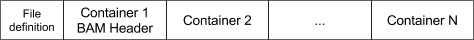
\includegraphics[width=356pt, height=31pt, keepaspectratio=true]{img/CRAMFileFormat2-1-fig001.png}
%%\caption{This should be the caption for \texttt{img/CRAMFileFormat2-1-fig001.png}.}
%%\end{figure}

Pic.1 CRAM file starts with a file definition followed by the BAM header and other 
containers.

Containers consist of one or more blocks. By convention, the BAM header is stored 
in the first container within a single block. This is known as the BAM header block.

%%\begin{figure}[htbp]
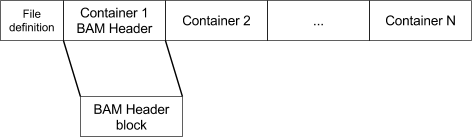
\includegraphics[width=354pt, height=103pt, keepaspectratio=true]{img/CRAMFileFormat2-1-fig002.png}
%%\caption{This should be the caption for \texttt{img/CRAMFileFormat2-1-fig002.png}.}
%%\end{figure}

Pic.2 The BAM header is stored in the first container.

Each container starts with a container header followed by one or more blocks. Each 
block starts with a block header. All data in CRAM is stored within blocks after 
the block header.

%%\begin{figure}[htbp]
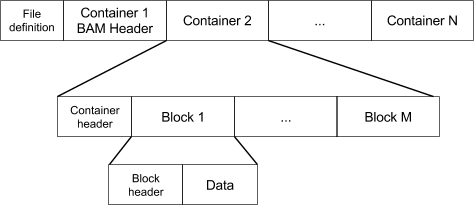
\includegraphics[width=356pt, height=154pt, keepaspectratio=true]{img/CRAMFileFormat2-1-fig003.png}
%%\caption{This should be the caption for \texttt{img/CRAMFileFormat2-1-fig003.png}.}
%%\end{figure}

Pic.3 Container and block structure. All data in CRAM files is stored in blocks.

The first block in each container is the compression header block:

%%\begin{figure}[htbp]
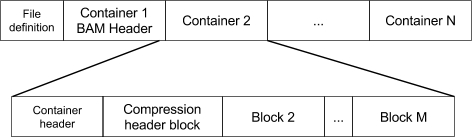
\includegraphics[width=354pt, height=103pt, keepaspectratio=true]{img/CRAMFileFormat2-1-fig004.png}
%%\caption{This should be the caption for \texttt{img/CRAMFileFormat2-1-fig004.png}.}
%%\end{figure}

Pic.4 Compression header is the first block in the container.

The blocks after the compression header are organised logically into slices. One 
slice may contain, for example, a contiguous region of alignment data. Slices begin 
with a slice header block and are followed by one or more data blocks:

%%\begin{figure}[htbp]
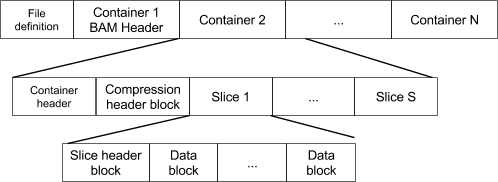
\includegraphics[width=374pt, height=137pt, keepaspectratio=true]{img/CRAMFileFormat2-1-fig005.png}
%%\caption{This should be the caption for \texttt{img/CRAMFileFormat2-1-fig005.png}.}
%%\end{figure}

Pic.5 Containers are logically organised into slices.

Data blocks are divided into core and external data blocks. Each slice must have 
at least one core data block immediately after the slice header block. The core 
data block may be followed by one or more external data blocks.

%%\begin{figure}[htbp]
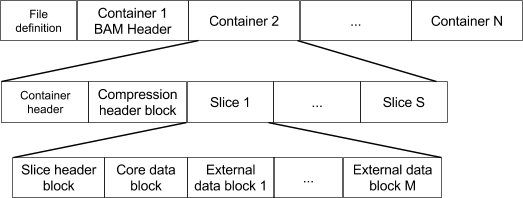
\includegraphics[width=392pt, height=149pt, keepaspectratio=true]{img/CRAMFileFormat2-1-fig006.png}
%%\caption{This should be the caption for \texttt{img/CRAMFileFormat2-1-fig006.png}.}
%%\end{figure}

Pic.5 Data blocks are divided into core and external data blocks. 

\section{\textbf{File definition}}

Each CRAM file starts with a fixed length (26 bytes) definition with the following 
fields:

\begin{tabular}{|l|l|l|}
\hline
\textbf{Data type} & \textbf{Name} & \textbf{Value}\tabularnewline
\hline
byte[4] & format magic number & CRAM (0x43 0x52 0x41 0x4d)\tabularnewline
\hline
unsigned byte & major format number & 3 (0x3)\tabularnewline
\hline
unsigned byte & minor format number & 0 (0x0)\tabularnewline
\hline
byte[20] & file id & CRAM file identifier (e.g. file name or SHA1 checksum)\tabularnewline
\hline
\end{tabular}

Valid CRAM \textit{major}.\textit{minor} version numbers are as follows:

\begin{itemize}
\item[\textit{1.0}]
The original public CRAM release.

\item[\textit{2.0}]
The first CRAM release implemented in both Java and C; tidied up
implementation vs specification differences in \textit{1.0}.

\item[\textit{2.1}]
Gained end of file markers; compatible with \textit{2.0}.

\item[\textit{3.0}]
Additional compression methods; header and data checksums;
improvements for unsorted data.
\end {itemize}

\section{\textbf{Container structure}}

The file definition is followed by one or more containers with the following header 
structure where the container content is stored in the `blocks' field:

\begin{tabular}{|l|>{\raggedright}p{120pt}|>{\raggedright}p{260pt}|}
\hline
\textbf{Data type} & \textbf{Name} & \textbf{Value}
\tabularnewline
\hline
int32 & length & byte size of the container data (blocks)\tabularnewline
\hline
itf8 & reference sequence id & reference sequence identifier  or\linebreak{}
-1 for unmapped reads\linebreak{}
-2 for multiple reference sequences\tabularnewline
\hline
itf8 & starting position on the reference & the alignment start position or\linebreak{}
0 for unmapped reads\tabularnewline
\hline
itf8 & alignment span & the length of the alignment or\linebreak{}
0 for unmapped reads\tabularnewline
\hline
itf8 & number of records & number of records in the container\tabularnewline
\hline
ltf8 & record counter & 1-based sequential index of records in the file/stream.\tabularnewline
\hline
ltf8 & bases & number of read bases\tabularnewline
\hline
itf8 & number of blocks & the number of blocks\tabularnewline
\hline
itf8[ ] & landmarks & Each integer value of this array is a byte offset into the 
blocks byte array. Landmarks are used for random access indexing.\tabularnewline
\hline
int & crc32 & CRC32 hash of the all the preceding bytes in the container.\tabularnewline
\hline
byte[ ] & blocks & The blocks contained within the container.\tabularnewline
\hline
\end{tabular}

\subsection{\textbf{CRAM header in the first container}}

The first container in the CRAM file contains the BAM header in an optionally
compressed block. Only gzip is allowed as compression method for this block. BAM
header is terminated with \textbackslash{}0 byte and any extra bytes in the
block can be used to expand the BAM header. For example when updating @SQ
records additional space may be required for the BAM header. It is recommended
to reserve 50\% more space in the CRAM header block than it is required by the
BAM header.

\section{\textbf{Block structure}}

Containers consist of one or more blocks. Block compression is applied independently 
and in addition to any encodings used to compress data within the block. The block 
have the following header structure with the data stored in the `block data' field:

\begin{tabular}{|l|>{\raggedright}p{120pt}|>{\raggedright}p{260pt}|}
\hline
\textbf{Data type} & \textbf{Name} & \textbf{Value}
\tabularnewline
\hline
byte & method & the block compression method: \linebreak{}
0: raw (none)*\linebreak{}
1: gzip\linebreak{}
2: bzip2\linebreak{}
3: lzma\linebreak{}
4: rans\tabularnewline
\hline
byte & block content type id & the block content type identifier\tabularnewline
\hline
itf8 & block content id & the block content identifier used to associate external 
data blocks with data series\tabularnewline
\hline
itf8 & size in bytes* & size of the block data after applying block compression\tabularnewline
\hline
itf8 & raw size in bytes* & size of the block data before applying block compression\tabularnewline
\hline
byte[ ] & block data & the data stored in the block:\linebreak{}
$\bullet$ bit stream of CRAM records (core data block)\linebreak{}
$\bullet$ byte stream (external data block)\linebreak{}
$\bullet$ additional fields ( header blocks)\tabularnewline
\hline
byte[4] & CRC32 & CRC32 hash value for all preceding bytes in the block\tabularnewline
\hline
\end{tabular}

* Note on raw method: both compressed and raw sizes must be set to the same value.

\subsection{\textbf{Block content types}}

CRAM has the following block content types:

\begin{tabular}{|>{\raggedright}p{143pt}|>{\raggedright}p{45pt}|>{\raggedright}p{116pt}|>{\raggedright}p{114pt}|}
\hline
\textbf{Block content type} & \textbf{Block content type id} & \textbf{Name} & \textbf{Contents}\tabularnewline
\hline
FILE\_HEADER & 0 & BAM header block & BAM header\tabularnewline
\hline
COMPRESSION\_HEADER & 1 & Compression header block & See specific section\tabularnewline
\hline
MAPPED\_SLICE\_HEADER & 2 & Slice header block & See specific section\tabularnewline
\hline
 & 3 &  & reserved\tabularnewline
\hline
EXTERNAL\_DATA & 4 & external data block & data produced by external encodings\tabularnewline
\hline
CORE\_DATA & 5 & core data block & bit stream of all encodings except for external\tabularnewline
\hline
\end{tabular}


\subsection{\textbf{Block content id}}

Block content id is used to distinguish between external blocks in the same slice. 
Each external encoding has an id parameter which must be one of the external block 
content ids. For external blocks the content id is a positive integer. For all 
other blocks content id should be 0. Consequently, all external encodings must 
not use content id less than 1. 

\subsubsection*{Data blocks}

Data is stored in data blocks. There are two types of data blocks: core data blocks 
and external data blocks.The difference between core and external data blocks is 
that core data blocks consist of data series that are compressed using bit encodings 
while the external data blocks are byte compressed. One core data block and any 
number of external data blocks are associated with each slice.

Writing to and reading from core and external data blocks is organised through 
CRAM records. Each data series is associated with an encoding. In case of external 
encoding the block content id is used to identify the block where the data series 
is stored. Please note that external blocks can have multiple data series associated 
with them; in this case the values from these data series will be interleaved. 


\subsection{\textbf{BAM header block}}

The BAM header is stored in a single block within the first container. 

The following constraints apply to the BAM header: 

\begin{itemize}
\item The SQ:MD5 checksum is required unless the reference sequence has been embedded 
into the file.

\item At least one RG record is required.

\item The HD:SO sort order is always POS.
\end{itemize}

\subsection{\textbf{Compression header block}}
\label{subsec:compression-header}

The compression header block consists of 3 parts: preservation map, data series 
encoding map and tag encoding map.

\subsubsection*{Preservation map}

The preservation map contains information about which data was preserved in the 
CRAM file. It is stored as a map with byte[2] keys:

\begin{tabular}{|l|l|>{\raggedright}p{100pt}|>{\raggedright}p{220pt}|}
\hline
\textbf{Key} & \textbf{Value data type} & \textbf{Name} & \textbf{Value}\tabularnewline
\hline
RN & bool & read names included & true if read names are preserved for all reads\tabularnewline
\hline
AP & bool & AP data series delta & true if AP data series is delta, false otherwise\tabularnewline
\hline
RR & bool & reference required & true if reference sequence is required to restore 
the data completely\tabularnewline
\hline
SM & byte[5] & substitution matrix & substitution matrix\tabularnewline
\hline
TD & byte[ ] & tag ids dictionary & a list of lists of tag ids, see tag encoding 
section\tabularnewline
\hline
\end{tabular}

\subsubsection*{Data series encodings}

Each data series has an encoding. These encoding are stored in a map with byte[2] 
keys and are decoded in approximately this order\footnote{The precise order is defined in section~\ref{sec:record}.}:

\begin{threeparttable}[t]
\begin{tabular}{|l|l|>{\raggedright}p{100pt}|>{\raggedright}p{220pt}|}
\hline
\textbf{Key} & \textbf{Value data type} & \textbf{Name} & \textbf{Value}\tabularnewline
\hline
BF & encoding\texttt{<}int\texttt{>} & BAM bit flags & see separate section\tabularnewline
\hline
CF & encoding\texttt{<}int\texttt{>} & CRAM bit flags & see specific section\tabularnewline
\hline
RI & encoding\texttt{<}int\texttt{>} & reference id & record reference id from
the BAM file header\tabularnewline
\hline
RL & encoding\texttt{<}int\texttt{>} & read lengths & read lengths\tabularnewline
\hline
AP & encoding\texttt{<}int\texttt{>} & in-seq positions & 0-based alignment start
delta from previous record *\tabularnewline
\hline
RG & encoding\texttt{<}int\texttt{>} & read groups & read groups. Special value 
`-1' stands for no group.\tabularnewline
\hline
RN\tnote{a} & encoding\texttt{<}byte[ ]\texttt{>} & read names & read names\tabularnewline
\hline
MF & encoding\texttt{<}int\texttt{>} & next mate bit flags & see specific section\tabularnewline
\hline
NS & encoding\texttt{<}int\texttt{>} & next fragment reference sequence id & reference 
sequence ids for the next fragment \tabularnewline
\hline
NP & encoding\texttt{<}int\texttt{>} & next mate alignment start & alignment positions 
for the next fragment\tabularnewline
\hline
TS & encoding\texttt{<}int\texttt{>} & template size & template sizes\tabularnewline
\hline
NF & encoding\texttt{<}int\texttt{>} & distance to next fragment & number of records
to the next fragment\tnote{b}\tabularnewline
\hline
TL\tnote{c} & encoding\texttt{<}int\texttt{>} & tag ids  & list of tag ids, see tag encoding
section\tabularnewline
\hline
FN & encoding\texttt{<}int\texttt{>} & number of read features & number of read
features in each record\tabularnewline
\hline
FC & encoding\texttt{<}byte\texttt{>} & read features codes & see separate section\tabularnewline
\hline
FP & encoding\texttt{<}int\texttt{>} & in-read positions & positions of the read
features\tabularnewline
\hline
DL & encoding\texttt{<}int\texttt{>} & deletion lengths & base-pair deletion lengths\tabularnewline
\hline
BB & encoding\texttt{<}byte[ ]\texttt{>} & stretches of bases & bases\tabularnewline
\hline
QQ & encoding\texttt{<}byte[ ]\texttt{>} & stretches of quality scores & quality scores\tabularnewline
\hline
BS & encoding\texttt{<}byte\texttt{>} & base substitution codes & base substitution
codes\tabularnewline
\hline
IN & encoding\texttt{<}byte[ ]\texttt{>} & insertion & inserted bases\tabularnewline
\hline
RS & encoding\texttt{<}int\texttt{>} & reference skip length & number of skipped 
bases for the `N' read feature\tabularnewline
\hline
PD & encoding\texttt{<}int\texttt{>} & padding & number of padded bases\tabularnewline
\hline
HC & encoding\texttt{<}int\texttt{>} & hard clip & number of hard clipped bases\tabularnewline
\hline
SC & encoding\texttt{<}byte[ ]\texttt{>} & soft clip & soft clipped bases\tabularnewline
\hline
MQ & encoding\texttt{<}int\texttt{>} & mapping qualities & mapping quality scores\tabularnewline
\hline
BA & encoding\texttt{<}byte\texttt{>} & bases & bases\tabularnewline
\hline
QS & encoding\texttt{<}byte\texttt{>} & quality scores & quality scores\tabularnewline
\hline
\end{tabular}

\begin{tablenotes}
\item{a} Note RN this is decoded after MF if the record is detached from the mate and we are attempting to auto-generate read names.
\item{b} The count is reset for each slice so NF can only refer to a record later within this slice.
\item{c} TL is followed by decoding the tag values themselves, in order of appearance in the tag dictionary.
\end{tablenotes}
\end{threeparttable}

\subsubsection*{Tag encodings}
\label{subsubsec:tags}

The tag dictionary (TD) describes the unique combinations of tag id / type that occur on each alignment record.
For example if we search the id / types present in each record and find only two combinations -- X1:i BC:Z SA:Z: and X1:i: BC:Z -- then we have two dictionary entries in the TD map.

Let $L_{i}=\{T_{i0}, T_{i1}, \ldots, T_{ix}\}$ be a list of all tag ids for a record $R_{i}$, where $i$ is the sequential record index and $T_{ij}$ denotes $j$-th tag id in the record.
The list of unique $L_{i}$ is stored as the TD value in the preservation map.
Maintaining the order is not a requirement for encoders (hence ``combinations''), but it is permissible and thus different permutations, each encoded with their own elements in TD, should be supported by the decoder.
Each $L_{i}$ element in TD is assigned a sequential integer number starting with 0.
These integer numbers are referred to by the TL data series.
Using TD, an integer from the TL data series can be mapped back into a list of tag ids.
Thus per alignment record we only need to store tag values and not their ids and types.

The TD is written as a byte array consisting of $L_{i}$ values separated with \textbackslash{}0.
Each $L_{i}$ value is written as a concatenation of 3 byte $T_{ij}$ elements: tag id followed by BAM tag type code (one of A, c, C, s, S, i, I, f, F, Z, H or B, as described in the SAM specification).
For example the TD for tag lists X1:i BC:Z SA:Z and X1:i BC:Z may be encoded as X1CBCZSAZ\textbackslash{}0X1CBCZ\textbackslash{}0, with X1C indicating a 1 byte unsigned value for tag X1.

\subsubsection*{Tag values}

The encodings used for different tags are stored in a map.
The key is 3 bytes formed from the BAM tag id and type code, matching the TD dictionary described above.
Unlike the Data Series Encoding Map, the key is stored in the map as an ITF8 encoded integer, constructed using $(char1<<16) + (char2<<8) + type$.
For example, the 3-byte representation of OQ:Z is \{0x4F, 0x51, 0x5A\} and these bytes are intepreted as the integer key 0x004F515A, leading to an ITF8 byte stream \{0xE0, 0x4F, 0x51, 0x5A\}.

\begin{tabular}{|l|l|l|>{\raggedright}p{160pt}|}
\hline
\textbf{Key} & \textbf{Value data type} & \textbf{Name} & \textbf{Value}
\tabularnewline
\hline
TAG ID 1:TAG TYPE 1 & encoding\texttt{<}byte[ ]\texttt{>} & read tag 1 & tag values
(names and types are available in the data series code)\tabularnewline
\hline
... &  & ... & ...\tabularnewline
\hline
TAG ID N:TAG TYPE N & encoding\texttt{<}byte[ ]\texttt{>} & read tag N & ...\tabularnewline
\hline
\end{tabular}

Note that tag values are encoded as array of bytes. The routines to convert tag 
values into byte array and back are the same as in BAM with the exception of value 
type being captured in the tag key rather in the value.
Hence consuming 1 byte for types `C' and `c', 2 bytes for types `S' and `s', 4 bytes for types `I', `i' and `f', and a variable number of bytes for types `H', `Z' and `B'.

\subsection{\textbf{Slice header block}}

The slice header block is never compressed (block method=raw). For reference mapped 
reads the slice header also defines the reference sequence context of the data 
blocks associated with the slice. Mapped and unmapped reads can be stored within 
the same slice similarly to BAM file. Slices with unsorted reads must not contain 
any other types of reads.

The slice header block contains the following fields.

\begin{tabular}{|l|l|>{\raggedright}p{200pt}|}
\hline
\textbf{Data type} & \textbf{Name} & \textbf{Value}\tabularnewline
\hline
itf8 & reference sequence id & reference sequence identifier or -1 for unmapped 
or unsorted reads\tabularnewline
\hline
itf8 & alignment start & the alignment start position or -1 for unmapped or unsorted 
reads\tabularnewline
\hline
itf8 & alignment span & the length of the alignment or 0 for unmapped or unsorted 
reads\tabularnewline
\hline
itf8 & number of records & the number of records in the slice\tabularnewline
\hline
ltf8 & record counter & 1-based sequential index of records in the file/stream\tabularnewline
\hline
itf8 & number of blocks & the number of blocks in the slice\tabularnewline
\hline
itf8[ ] & block content ids & block content ids of the blocks in the slice\tabularnewline
\hline
itf8 & embedded reference bases block content id & block content id for the embedded 
reference sequence bases or -1 for none\tabularnewline
\hline
byte[16] & reference md5 & MD5 checksum of the reference bases within the slice 
boundaries or 16 \textbackslash{}0 bytes for unmapped or unsorted reads\tabularnewline
\hline
byte[] & optional tags & a series of tag,type,value tuples encoded as
per BAM auxiliary fields.\tabularnewline
\hline
\end{tabular}

The optional tags are encoded in the same manner as BAM tags.  I.e. a
series of binary encoded tags concatenated together where each tag
consists of a 2 byte key (matching [A-Za-z][A-Za-z0-9]) followed by a
1 byte type ([AfZHcCsSiIB]) followed by a string of bytes in a format
defined by the type.

Tags starting in a capital letter are reserved while lowercase ones or
those starting with X, Y or Z are user definable.  Any tag not
understood by a decoder should be skipped over without producing an
error.

At present no tags are defined.

% Details omitted until we fully work through all the corner cases,
% such as seq/qual of *.
%
% Reserved tags are defined as follows:
% 
% \begin{tabular}{|l|l|>{\raggedright}p{325pt}|}
% \hline
% \textbf{Tag type} & \textbf{BAM format} & \textbf{Meaning}\tabularnewline
% \hline
% BD & i & Sum over all reads of the CRC32 hash of sequence base.  This
% may be used to validate round-trips in and out of CRAM.
% calls\tabularnewline
% \hline
% SD & i & Sum over all reads of the CRC32 hash of quality scores. (If
% the quality string is ``*'' in SAM then the hash is of the BAM encoded
% version - a string of bytes with value 255.)\tabularnewline
% \hline
% \end{tabular}


\subsection{\textbf{Core data block}}

A core data block is a bit stream (most significant bit first) consisting of one 
or more CRAM records. Please note that one byte could hold more then one CRAM record 
as a minimal CRAM record could be just a few bits long. The core data block has 
the following fields:

\begin{tabular}{|l|>{\raggedright}p{120pt}|>{\raggedright}p{260pt}|}
\hline
\textbf{Data type} & \textbf{Name} & \textbf{Value}
\tabularnewline
\hline
bit[ ] & CRAM record 1 & The first CRAM record\tabularnewline
\hline
... & ... & ...\tabularnewline
\hline
bit[ ] & CRAM record N & The Nth CRAM record \tabularnewline
\hline
\end{tabular}

\subsection{\textbf{External data block}}

Relationship between core data block and external data blocks is shown in the following 
picture: 

%%\begin{figure}[htbp]
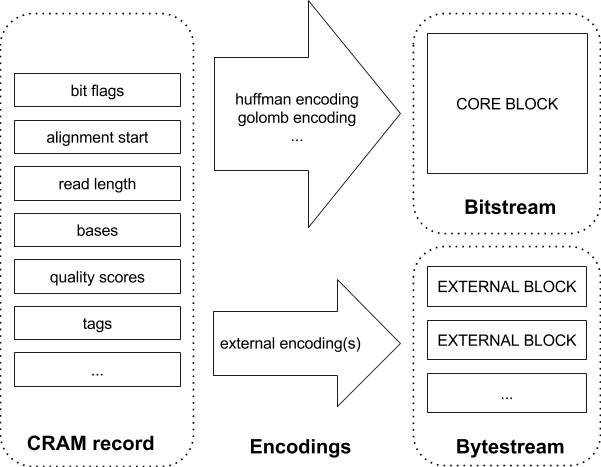
\includegraphics[width=451pt, height=350pt, keepaspectratio=true]{img/CRAMFileFormat2-1-fig007.png}
%%\caption{This should be the caption for \texttt{img/CRAMFileFormat2-1-fig007.png}.}
%%\end{figure}

Pic.3 Relationship between core data block and external data blocks.

The picture shows how a CRAM record (on the left) is partially written to core 
data block while the other fields are stored in two external data blocks. The specific 
encodings are presented only for demonstration purposes, the main point here is 
to distinguish between bit encodings whose output is always stored in core data 
block and the external encoding which simply stored the bytes into external data 
blocks.

\section{\textbf{End of file marker}}

A special container is used to mark the end of a file or stream. It is required in version 3 or later. The idea is to provide an easy and a quick way to detect that a CRAM file or stream is complete. The marker is basically an empty container with ref seq id set to -1 (unaligned) and alignment 
start set to 4542278.

Here is a complete content of the EOF container explained in detail:

\begin{tabular}{|l|l|>{\raggedright}p{150pt}|>{\raggedright}p{180pt}|}
\hline
\textbf{hex bytes} & \textbf{data type} & \textbf{decimal value} & \textbf{field 
name}\tabularnewline
\hline
\multicolumn{4}{|l|}{\textit{Container header}}\tabularnewline
\hline
0f 00 00 00 & integer & 15 & size of blocks data\tabularnewline
\hline
ff ff ff ff 0f & itf8 & -1 & ref seq id\tabularnewline
\hline
e0 45 4f 46 & itf8 & 4542278 & alignment start\tabularnewline
\hline
00 & itf8 & 0 & alignment span\tabularnewline
\hline
00 & itf8 & 0 & number of records\tabularnewline
\hline
00 & itf8 & 0 & global record counter\tabularnewline
\hline
00 & itf8 & 0 & bases\tabularnewline
\hline
01 & itf8 & 1 & block count\tabularnewline
\hline
00 & array & 0 & landmarks\tabularnewline
\hline
05 bd d9 4f & integer & 1339669765 & container header CRC32\tabularnewline
\hline
\multicolumn{4}{|l|}{\textit{Compression header block}}\tabularnewline
\hline
00 & byte & 0 (RAW) & compression method\tabularnewline
\hline
01 & byte & 1 (COMPRESSION\_HEADER) & block content type\tabularnewline
\hline
00 & itf8 & 0 & block content id\tabularnewline
\hline
06 & itf8 & 6 & compressed size\tabularnewline
\hline
06 & itf8 & 6 & uncompressed size\tabularnewline
\hline
\multicolumn{4}{|l|}{\textit{Compression header}}\tabularnewline
\hline
01 & itf8 & 1 & preservation map byte size\tabularnewline
\hline
00 & itf8 & 0 & preservation map size\tabularnewline
\hline
01 & itf8 & 1 & encoding map byte size\tabularnewline
\hline
00 & itf8 & 0 & encoding map size\tabularnewline
\hline
01 & itf8 & 1 & tag encoding byte size\tabularnewline
\hline
00 & itf8 & 0 & tag encoding map size\tabularnewline
\hline
ee 63 01 4b & integer & 1258382318 & block CRC32\tabularnewline
\hline
\end{tabular}

When compiled together the EOF marker is 38 bytes long and in hex representation 
is:

0f 00 00 00 ff ff ff ff 0f e0 45 4f 46 00 00 00 00 01 00 05 bd d9 4f 00 01 00 06 06 01 00 01 00 01 00 ee 63 01 4b

\section{\textbf{Record structure}}
\label{sec:record}

CRAM record is based on the SAM record but has additional features allowing for 
more efficient data storage.  In contrast to BAM record CRAM record uses bits as 
well as bytes for data storage. This way, for example, various coding techniques 
which output variable length binary codes can be used directly in CRAM. On the 
other hand, data series that do not require binary coding can be stored separately 
in external blocks with some other compression applied to them independently.

As CRAM data series may be interleaved within the same blocks\footnote{Interleaving can sometimes provide better compression, however it also adds dependency between types of data meaning it is not possible to selectively decode one data series if it co-locates with another data series in the same block.} understanding the order in which CRAM data series must be decoded is vital.

The overall flowchart is below, with more detailed description in the subsequent sections.

\algnewcommand\algorithmicto{\text{ \textbf{to} }}

\subsection{\textbf{CRAM record}}

Both mapped and unmapped reads start with the following fields. Please note that 
the data series type refers to the logical data type and the data series name corresponds 
to the data series encoding map.

\begin{tabular}{|>{\raggedright}p{70pt}|>{\raggedright}p{75pt}|>{\raggedright}p{90pt}|>{\raggedright}p{171pt}|}
\hline
\textbf{Data series type} & \textbf{Data series name} & \textbf{Field} & \textbf{Description}\tabularnewline
\hline
int & BF & BAM bit flags & see BAM bit flags below\tabularnewline
\hline
int & CF & CRAM bit flags & see CRAM bit flags below\tabularnewline
\hline
- & - & Positional data & See section \ref{subsec:positions}\tabularnewline
\hline
- & - & Read names & See section \ref{subsec:names}\tabularnewline
\hline
- & - & Mate records & See section \ref{subsec:mate}\tabularnewline
\hline
- & - & Auxiliary tags & See section \ref{subsec:tags}\tabularnewline
\hline
- & - & Sequences & See sections \ref{subsec:mapped} and \ref{subsec:unmapped}\tabularnewline
\hline
\end{tabular}

\subsubsection*{\textbf{BAM bit flags (BF data series)}}

The following flags are duplicated from the SAM and BAM specification, with identical meaning.
Note however some of these flags can be derived during decode, so may be omitted in the CRAM file and the bits computed based on both reads of a pair-end library residing within the same slice.

\begin{threeparttable}[t]
\begin{tabular}{|>{\raggedright}p{144pt}|>{\raggedright}p{144pt}|>{\raggedright}p{144pt}|}
\hline
\textbf{Bit flag} & \textbf{Comment} & \textbf{Description}\tabularnewline
\hline
0x1 &  & template having multiple segments in sequencing\tabularnewline
\hline
0x2 &  & each segment properly aligned according to the aligner\tabularnewline
\hline
0x4 &  & segment unmapped\tnote{a}\tabularnewline
\hline
0x8 & calculated\tnote{b}\ \ or stored in the mate's info & next segment in template unmapped\tabularnewline
\hline
0x10 &  & SEQ being reverse complemented\tabularnewline
\hline
0x20 & calculated\tnote{b}\ \ or stored in the mate's info & SEQ of the next segment in the
template being reversed\tabularnewline
\hline
0x40 &  & the first segment in the template\tnote{c}\tabularnewline
\hline
0x80 &  & the last segment in the template\tnote{c}\tabularnewline
\hline
0x100 &  & secondary alignment\tabularnewline
\hline
0x200 &  & not passing quality controls\tabularnewline
\hline
0x400 &  & PCT or optical duplicate\tabularnewline
\hline
0x800 &  & Supplementary alignment\tabularnewline
\hline
\end{tabular}
\begin{tablenotes}
\item[a] Bit 0x4 is the only reliable place to tell whether the read is unmapped.  If 0x4 is set, no assumptions may be made about bits 0x2, 0x100 and 0x800.
\item[b] For segments within the same slice.
\item[c] Bits 0x40 and 0x80 reflect the read ordering within each template inherent in the sequencing technology used, which may be independent from the actual mapping orientation.
If 0x40 and 0x80 are both set, the read is part of a linear template (one where the template sequence is expected to be in a linear order), but it is neither the first nor the last read.
If both 0x40 and 0x80 are unset, the index of the read in the template is unknown.
This may happen for a non-linear template (such as one constructed by stitching together other templates) or when this information is lost during data processing.
\end{tablenotes}
\end{threeparttable}

\subsubsection*{\textbf{CRAM bit flags (CF data series)}}

The CRAM bit flags (also known as compression bit flags) expressed as an integer represent the CF data series. 
The following compression flags are defined for each CRAM read record:

\begin{tabular}{|>{\raggedright}p{39pt}|>{\raggedright}p{150pt}|>{\raggedright}p{242pt}|}
\hline
\textbf{Bit flag} & \textbf{Name} & \textbf{Description}\tabularnewline
\hline
0x1 & quality scores stored as array & quality scores can be stored as read features
or as an array similar to read bases.\tabularnewline
\hline
0x2 & detached & mate information is stored verbatim (e.g. because the pair spans multiple slices or the fields differ to the CRAM computed method)\tabularnewline
\hline
0x4 & has mate downstream & tells if the next segment should be expected further
in the stream\tabularnewline
\hline
0x8 & decode sequence as ``*'' & informs the decoder that the sequence
is unknown and that any encoded reference differences are present only to
recreate the CIGAR string.\tabularnewline
\hline
\end{tabular}


The following pseudocode describes the general process of decoding an entire CRAM record.
The sequence data itself is in one of two encoding formats depending on whether the record is aligned (mapped).

\subsubsection*{\textbf{Decode pseudocode}}
\newlength{\maxwidth}
\newcommand{\algalign}[2] % #1 = text to left, #2 = text to right
{\makebox[\maxwidth][l]{$#1{}$}${}#2$}

\begin{algorithmic}[1]
\Procedure{DecodeRecord}{}
\settowidth{\maxwidth}{CRAM\_flags\quad}
\State \algalign{BAM\_flags}{\gets}  \Call{ReadItem}{BF, Integer}
\State \algalign{CRAM\_flags}{\gets} \Call{ReadItem}{CF, Integer}
\State \Call{DecodePositions}{}\Comment{See section \ref{subsec:positions}}
\State \Call{DecodeNames}{}\Comment{See section \ref{subsec:names}}
\State \Call{DecodeMateData}{}\Comment{See section \ref{subsec:mate}}
\State \Call{DecodeTagData}{}\Comment{See section \ref{subsec:tags}}
\Statex

\If{$(BF$ AND $4) \ne 0$}\Comment{Unmapped flag}
  \State \Call{DecodeMappedRead}{}\Comment{See section \ref{subsec:mapped}}
\Else
  \State \Call{DecodeUnmappedRead}{}\Comment{See section \ref{subsec:unmapped}}
\EndIf
\EndProcedure
\end{algorithmic}

\subsection{\textbf{CRAM positional data}}
\label{subsec:positions}

Following the bit-wise BAM and CRAM flags, CRAM encodes positional related data including reference, alignment positions and length, and read-group.
Positional data is stored for both mapped and unmapped sequences, as unmapped data may still be ``placed'' at a specific location in the genome (without being aligned).
Typically this is done to keep a sequence pair (paired-end or mate-pair sequencing libraries) together when one of the pair aligns and the other does not.

The AP data series is delta encoded for reads mapped to a position-sorted slice containing data from a single reference, and as a normal integer value in all other cases.

\begin{tabular}{|>{\raggedright}p{70pt}|>{\raggedright}p{75pt}|>{\raggedright}p{90pt}|>{\raggedright}p{171pt}|}
\hline
\textbf{Data series type} & \textbf{Data series name} & \textbf{Field} & \textbf{Description}\tabularnewline
\hline
int & RI & ref id & reference sequence id (only present in multiref slices)\tabularnewline
\hline
int & RL & read length & the length of the read\tabularnewline
\hline
int & AP & alignment start & the alignment start position\tabularnewline
\hline
int & RG & read group & the read group identifier expressed as the N\textsuperscript{th} record in the header, starting from 0 with -1 for no group\tabularnewline
\hline
\end{tabular}

\vskip 20pt
\begin{algorithmic}[1]
\Procedure{DecodePositions}{}
\If{$slice\_header.reference\_sequence\_id = -2$}
  \State $reference\_id\gets$ \Call{ReadItem}{RI, Integer}
\Else
  \State $reference\_id\gets slice\_header.reference\_sequence\_id$
\EndIf
\State $read\_length \gets$ \Call{ReadItem}{RL, Integer}
\If{$container\_pmap.AP\_delta \ne 0$}
    \State Initialise $last\_position$ to 0 if first record in slice
    \State $alignment\_position \gets$ \Call{ReadItem}{AP, Integer} + $last\_position$
    \State $last\_position \gets alignment\_position$
\Else
    \State $alignment\_position \gets$ \Call{ReadItem}{AP, Integer}
\EndIf
\State $read\_group \gets$ \Call{ReadItem}{RG, Integer}
\EndProcedure
\end{algorithmic}

\subsection{Read names (RN data series)}
\label{subsec:names}

Read names can be preserved in the CRAM format, but this is optional and is governed by the \texttt{RN} preservation map key in the container compression header. See section \ref{subsec:compression-header}.
When read names are not preserved the CRAM decoder should generate names, typically based on the file name and a numeric ID of the read using the record counter field of the slice header block.
Note read names may still be preserved even when the \texttt{RN} compression header key indicates otherwise, such as where a read is part of a read-pair and the pair spans multiple slices.
In this situation the record will be marked as detached (see the CF data series) and the mate data below (section \ref{subsec:mate}) will contain the read name.

\begin{tabular}{|>{\raggedright}p{70pt}|>{\raggedright}p{75pt}|>{\raggedright}p{90pt}|>{\raggedright}p{171pt}|}
\hline
\textbf{Data series type} & \textbf{Data series name} & \textbf{Field} & \textbf{Description}\tabularnewline
\hline
byte[] & RN & read names & read names\tabularnewline
\hline
\end{tabular}

\vskip 20pt
\begin{algorithmic}[1]
\Procedure{DecodeNames}{}
\If{$container\_pmap.read\_names\_included = 1$}
  \State $read\_name \gets$ \Call{ReadItem}{RN, Byte[]}
\Else
  \State $read\_name \gets$ \Call{GenerateName}{}
\EndIf
\Statex
\EndProcedure
\end{algorithmic}

\subsection{\textbf{Mate record}}
\label{subsec:mate}

There are two ways in which mate information can be preserved in CRAM: number of records downstream (distance, within this slice) to the next fragment in the template and a special mate record if the next fragment is not in the current slice.
In the latter case the record is labelled as ``detached'', see the CF data series.

For mates within the slice only the distance is captured, and only for the first record.  The mate has neither detached nor downstream flags set in the CF data series.

\begin{tabular}{|>{\raggedright}p{68pt}|>{\raggedright}p{115pt}|>{\raggedright}p{228pt}|}
\hline
\textbf{Data series type} & \textbf{Data series name} & \textbf{Description}\tabularnewline
\hline
int & NF & the number of records to the next fragment\tabularnewline
\hline
\end{tabular}

In the above case, the NS (mate reference name), NP (mate position) and TS (template size) fields for both records should be derived once the mate has also been decoded.
Mate reference name and position are obvious and simply copied from the mate.
The template size is computed using the method described in the SAM specification; the inclusive distance from the leftmost to rightmost mapped bases with the sign being positive for the leftmost record and negative for the rightmost record.

If the next fragment is not found within this slice then the following structure is included into the CRAM record.
Note there are cases where read-pairs within the same slice may be marked as detached and use this structure, such as to store mate-pair information that does not match the algorithm used by CRAM for computing the mate data on-the-fly.

\begin{tabular}{|>{\raggedright}p{66pt}|>{\raggedright}p{117pt}|>{\raggedright}p{228pt}|}
\hline
\textbf{Data series type} & \textbf{Data series name} & \textbf{Description}\tabularnewline
\hline
int & MF & next mate bit flags, see table below\tabularnewline
\hline
byte[ ] & RN & the read name (if and only if not known already)\tabularnewline
\hline
int & NS & mate reference sequence identifier \tabularnewline
\hline
int & NP & mate alignment start position \tabularnewline
\hline
int & TS & the size of the template (insert size)\tabularnewline
\hline
\end{tabular}

\subsubsection*{Next mate bit flags (MF data series)}

The next mate bit flags expressed as an integer represent the MF data series.
These represent the missing bits we excluded from the BF data series (when compared to the full SAM/BAM flags).
The following bit flags are defined:

\begin{tabular}{|>{\raggedright}p{47pt}|>{\raggedright}p{134pt}|>{\raggedright}p{250pt}|}
\hline
\textbf{Bit flag} & \textbf{Name} & \textbf{Description}\tabularnewline
\hline
0x1 & mate negative strand bit & the bit is set if the mate is on the negative
strand\tabularnewline
\hline
0x2 & mate mapped bit & the bit is set if the mate is mapped\tabularnewline
\hline
\end{tabular}


\subsubsection*{\textbf{Decode mate pseudocode}}

In the following pseudocode we are assuming the current record is $this$ and its mate is $next\_frag$.

\begin{algorithmic}[1]
\Procedure{DecodeMateData}{}
\If{$CF$ AND $2$}\Comment{Detached from mate}
  \State $mate\_flags\gets $ \Call{ReadItem}{MF,Integer}
  \If{$mate\_flags$ AND 1}
    \State $bam\_flags\gets bam\_flags$\ OR\ 0x20\Comment{Mate is reverse-complemented}
  \EndIf
  \If{$mate\_flags$ AND 2}
    \State $bam\_flags\gets bam\_flags$\ OR\ 0x08\Comment{Mate is unmapped}
  \EndIf
  \If{$container\_pmap.read\_names\_included \ne 1$}
    \State $read\_name \gets$ \Call{ReadItem}{RN, Byte[]}
  \EndIf
\settowidth{\maxwidth}{mate\_position\ }
\State \algalign{mate\_ref\_id}{\gets}  \Call{ReadItem}{NS, Integer}
\State \algalign{mate\_position}{\gets} \Call{ReadItem}{NP, Integer}
\State \algalign{template\_size}{\gets} \Call{ReadItem}{TS, Integer}
\ElsIf{$CF$ AND $4$}\Comment{Mate is downstream}
  \If{$next\_frag.bam\_flags$ AND 0x10}
    \State $this.bam\_flags \gets this.bam\_flags$\ OR\ 0x20\Comment{next segment reverse complemented}
  \EndIf
  \If{$next\_frag.bam\_flags$ AND 0x04}
    \State $this.bam\_flags \gets this.bam\_flags$\ OR\ 0x08\Comment{next segment unmapped}
  \EndIf
  \State $next\_frag\gets$ \Call{ReadItem}{NF,Integer}
  \State Resolve $mate\_ref\_id$ for $this$ record and $this+next\_frag$ once both have been decoded
  \State Resolve $mate\_position$ for $this$ record and $this+next\_frag$ once both have been decoded
  \State Find leftmost and rightmost mapped coordinate in records $this$ and $this+next\_frag$.
  \State For leftmost of $this$ and $this+next\_frag$ record: $template\_size\gets rightmost-leftmost+1$
  \State For rightmost of $this$ and $this+next\_frag$ record: $template\_size\gets -(rightmost-leftmost+1)$
\EndIf
\EndProcedure
\end{algorithmic}

Note as with the SAM specification a template may be permitted to have more than two alignment records.
In this case the ``mate'' for each record is considered to be the next record, with the mate for the last record being the first to form a circular list.
The above algorithm is a simplification that does not deal with this scenario.
The full method needs to observe when record $this+NF$ is also labelled as having an additional mate downstream.
One recommended approach is to resolve the mate information in a second pass, once the entire slice has been decoded.
The final segment in the mate chain needs to set $bam\_flags$ fields 0x20 and 0x08 accordingly based on the first segment.
This is also not listed in the above algorithm, for brevity.

\subsection{Auxiliary tags}
\label{subsec:tags}

Tags are encoded using a tag line (TL data series) integer into the tag dictionary (TD field in the compression header preservation map, see section \ref{subsec:compression-header}).
See section \ref{subsubsec:tags} for a more detailed description of this process.

\begin{tabular}{|>{\raggedright}p{70pt}|>{\raggedright}p{75pt}|>{\raggedright}p{90pt}|>{\raggedright}p{200pt}|}
\hline
\textbf{Data series type} & \textbf{Data series name} & \textbf{Field} & \textbf{Description}\tabularnewline
\hline
int & TL & tag line & an index into the tag dictionary (TD)\tabularnewline
\hline
* & ??? & tag name/type & 3 character key (2 tag identifier and 1 tag type), as specified by the tag dictionary\tabularnewline
\hline
\end{tabular}

\vskip 20pt
\begin{algorithmic}[1]
\Procedure{DecodeTagData}{}
\State $tag\_line\gets$ \Call{ReadItem}{TL,Integer}
\ForAll {$ele \in container\_pmap.tag\_dict(tag\_line)$}
  \State $name\gets$ first two characters of $ele$
  \State $tag(type)\gets$ last character of $ele$
  \State $tag(name)\gets$ \Call{ReadItem}{$ele$, Byte[]}
\EndFor
\EndProcedure
\end{algorithmic}

In the above procedure, $name$ is a two letter tag name and $type$ is one of the permitted types documented in the SAM/BAM specification.
Type is \texttt{c} (signed 8-bit integer), \texttt{C} (unsigned 8-bit integer), \texttt{s} (signed 16-bit integer), \texttt{S} (unsigned 16-bit integer), \texttt{i} (signed 32-bit integer), \texttt{I} (unsigned 32-bit integer), \texttt{f} (32-bit float), \texttt{Z} (nul-terminated string), \texttt{H} (nul-terminated string of hex digits) and \texttt{B} (binary data in array format with the first byte being one of c,C,s,S,i,I,f using the meaning above, a 32-bit integer for the number of array elements, followed by array data encoded using the specified format).  All integers are little endian encoded.

For example a SAM tag \texttt{MQ:i} has name \texttt{MQ} and type \texttt{i} and will be decoded using one of MQc, MQC, MQs, MQS, MQi and MQI data series depending on size and sign of the integer value.

\subsection{\textbf{Mapped reads}}
\label{subsec:mapped}

\subsubsection*{\textbf{Read feature records}}
\label{subsec:features}

Read features are used to store read details that are expressed using read coordinates 
(e.g. base differences respective to the reference sequence). The read feature 
records start with the number of read features followed by the read features themselves.
Finally the single mapping quality and per-base quality scores are stored.

\begin{threeparttable}[t]
\begin{tabular}{|>{\raggedright}p{88pt}|>{\raggedright}p{83pt}|>{\raggedright}p{85pt}|>{\raggedright}p{180pt}|}
\hline
\textbf{Data series type} & \textbf{Data series name} & \textbf{Field} & \textbf{Description}\tabularnewline
\hline
int & FN & number of read features & the number of read features\tabularnewline
\hline
int & FP & in-read-position\tnote{a} & position of the read feature\tabularnewline 
\hline
byte & FC & read feature code\tnote{a} & See feature codes below\tabularnewline
\hline
* & * & read feature data\tnote{a} & See feature codes below\tabularnewline
\hline
int & MQ & mapping qualities & mapping quality score\tabularnewline
\hline
byte[read length] & QS & quality scores & the base qualities, if preserved\tabularnewline
\hline
\end{tabular}
\begin{tablenotes}
\item[a] Repeated FN times, once for each read feature.
\end{tablenotes}
\end{threeparttable}

\subsubsection*{Read feature codes}

Each feature code has its own associated data series containing further information specific to that feature.
The following codes are used to distinguish variations in read coordinates:

\begin{tabular}{|>{\raggedright}p{91pt}|>{\raggedright}p{45pt}|>{\raggedright}p{72pt}|>{\raggedright}p{66pt}|>{\raggedright}p{132pt}|}
\hline
\textbf{Feature code} & \textbf{Id} & \textbf{Data series type} & \textbf{Data 
series name} & \textbf{Description}\tabularnewline
\hline
Bases & b (0x62) & byte[ ] & BB & a stretch of bases\tabularnewline
\hline
Scores & q (0x71) & byte[ ] & QQ & a stretch of scores\tabularnewline
\hline
% Neither C nor Java implementations generator nor can decode the 'A'
% feature code, but if they did they'd be BB/QQ and not BA/QS.  Best
% to omit it from published spec for now?
%
% Bases and scores & A (0x41) & byte[ ],byte[ ] & BB,QQ & A a stretch of bases and
% quality scores score\tabularnewline
% \hline
Read base & B (0x42) & byte,byte & BA,QS & A base and associated quality score\tabularnewline
\hline
Substitution & X (0x58) & byte & BS & base substitution codes, SAM operators X, 
M and =\tabularnewline
\hline
Insertion & I (0x49) & byte[ ] & IN & inserted bases, SAM operator I\tabularnewline
\hline
Deletion & D (0x44) & int & DL & number of deleted bases, SAM operator D\tabularnewline
\hline
Insert base & i (0x69) & byte & BA & single inserted base, SAM operator I\tabularnewline
\hline
Quality score & Q (0x51) & byte & QS & single quality score\tabularnewline
\hline
Reference skip & N (0x4E) & int & RS & number of skipped bases, SAM operator N\tabularnewline
\hline
Soft clip & S (0x53) & byte[ ] & SC & soft clipped bases, SAM operator S\tabularnewline
\hline
Padding & P (0x50) & int & PD & number of padded bases, SAM operator P\tabularnewline
\hline
Hard clip & H (0x48) & int & HC & number of hard clipped bases, SAM operator H\tabularnewline
\hline
\end{tabular}

\subsubsection*{Base substitution codes (BS data series)}

A base substitution is defined as a change from one nucleotide base (reference 
base) to another (read base) including N as an unknown or missing base. There are 
5 possible bases ACGTN, 4 possible substitutions for each base and 20 substitutions 
in total. Substitutions for the same reference base are assigned integer codes 
from 0 to 3 inclusive. To restore a base one would need to know its substitution 
code and the reference base. 

A base substitution matrix assigns integer codes to all possible substitutions. 

Substitution matrix is written as follows. Substitutions for a given reference 
base are sorted by their frequencies in descending order then assigned numbers 
from 0 to 3. Same-frequency ties are broken using alphabetical order. For example, 
let us assume the following substitution frequencies for base A: 

AC: 15\%

AG: 25\%

AT: 55\%

AN: 5\%

Then the substitution codes are: 

AC: 2

AG: 1

AT: 0

AN: 3

and they are written as a single byte, 10 01 00 11 = 147 decimal or 0x93 in this 
case. The whole substitution matrix is written as 5 bytes, one for each reference 
base in the alphabetical order: A, C, G, T and N.

Note: the last two bits of each substitution code are redundant but still required 
to simplify the reading. 

\subsubsection*{Decode mapped read pseudocode}

\begin{algorithmic}[1]
\Procedure{DecodeMappedRead}{}
  \State $feature\_number\gets$ \Call{ReadItem}{FN, Integer} 
  \For{$i\gets 1 \algorithmicto feature\_number$}
    \State \Call{DecodeFeature}{}
  \EndFor
  \State $mapping\_quality\gets$ \Call{ReadItem}{MQ, Integer} 
  \If{$container\_pmap.preserve\_quality\_scores$}
    \For{$i\gets 1 \algorithmicto read\_length$}
      \State $quality\_score\gets$ \Call{ReadItem}{QS, Integer} 
    \EndFor
  \EndIf
\EndProcedure
\Statex
\Procedure{DecodeFeature}{}
    \settowidth{\maxwidth}{feature\_position\ }
    \State \algalign{feature\_code}{\gets}       \Call{ReadItem}{FC, Integer} 
    \State \algalign{feature\_position}{\gets}   \Call{ReadItem}{FP, Integer} 
    \settowidth{\maxwidth}{substitution\_code\ }
    \If{$feature\_code = $`B'}
      \State \algalign{base}{\gets}              \Call{ReadItem}{BA, Byte}
      \State \algalign{quality\_score}{\gets}    \Call{ReadItem}{QS, Byte}
    \ElsIf{$feature\_code = $`X'}
      \State \algalign{substitution\_code}{\gets} \Call{ReadItem}{BS, Byte}
    \ElsIf{$feature\_code = $`I'}
      \State \algalign{inserted\_bases}{\gets}   \Call{ReadItem}{IN, Byte[]}
    \ElsIf{$feature\_code = $`S'}
      \State \algalign{softclip\_bases}{\gets}   \Call{ReadItem}{SC, Byte[]}
    \ElsIf{$feature\_code = $`H'}
      \State \algalign{hardclip\_length}{\gets}  \Call{ReadItem}{HC, Integer}
    \ElsIf{$feature\_code = $`P'}
      \State \algalign{pad\_length}{\gets}       \Call{ReadItem}{PD, Integer}
    \ElsIf{$feature\_code = $`D'}
      \State \algalign{deletion\_length}{\gets}  \Call{ReadItem}{DL, Integer}
    \ElsIf{$feature\_code = $`N'}
      \State \algalign{ref\_skip\_length}{\gets} \Call{ReadItem}{RS, Integer}
    \ElsIf{$feature\_code = $`i'}
      \State \algalign{base}{\gets}              \Call{ReadItem}{BA, Byte}
    \ElsIf{$feature\_code = $`b'}
      \State \algalign{bases}{\gets}             \Call{ReadItem}{BB, Byte[]}
    \ElsIf{$feature\_code = $`q'}
      \State \algalign{quality\_scores}{\gets}   \Call{ReadItem}{QQ, Byte[]}
    \ElsIf{$feature\_code = $`Q'}
      \State \algalign{quality\_score}{\gets}    \Call{ReadItem}{QS, Byte}
    \EndIf
\EndProcedure
\end{algorithmic}

\subsection{\textbf{Unmapped reads}}
\label{subsec:unmapped}

The CRAM record structure for unmapped reads has the following additional fields:

\begin{tabular}{|>{\raggedright}p{88pt}|>{\raggedright}p{83pt}|>{\raggedright}p{85pt}|>{\raggedright}p{180pt}|}
\hline
\textbf{Data series type} & \textbf{Data series name} & \textbf{Field} & \textbf{Description}\tabularnewline
\hline
byte[read length] & BA & bases & the read bases\tabularnewline
\hline
byte[read length] & QS & quality scores & the base qualities, if preserved\tabularnewline
\hline
\end{tabular}

\vskip20pt
\begin{algorithmic}[1]
\Procedure{DecodeUnmappedRead}{}
  \For{$i\gets 1 \algorithmicto read\_length$}
    \State $base\gets$ \Call{ReadItem}{BA, Byte}
  \EndFor
  \If{$container\_pmap.preserve\_quality\_scores$}
    \For{$i\gets 1 \algorithmicto read\_length$}
      \State $quality\_score\gets$ \Call{ReadItem}{QS, Byte}
    \EndFor
  \EndIf
\EndProcedure
\end{algorithmic}

\section{\textbf{Reference sequences}}

CRAM format is natively based upon usage of reference sequences even though in 
some cases they are not required. In contrast to BAM format CRAM format has strict 
rules about reference sequences. 

\begin{enumerate}
\item M5 (sequence MD5 checksum) field of @SQ sequence record in the BAM header is 
required and UR (URI for the sequence fasta optionally gzipped file) field is strongly 
advised. The rule for calculating MD5 is to remove any non-base symbols (like \textbackslash{}n, 
sequence name or length and spaces) and upper case the rest. Here are some examples: 

\texttt{> samtools faidx human\_g1k\_v37.fasta 1 \textbar{} grep -v '\textasciicircum{}>' \textbar{} tr -d '\textbackslash{}n' \textbar{} tr a-z A-Z \textbar{} md5sum -\\
1b22b98cdeb4a9304cb5d48026a85128  -}

\texttt{> samtools faidx human\_g1k\_v37.fasta 1:10-20 \textbar{}grep -v '\textasciicircum{}\texttt{>}' \textbar{}tr -d '\textbackslash{}n' \textbar{}tr a-z A-Z \textbar{}md5sum -\\
0f2a4865e3952676ffad2c3671f14057  -}

Please note that the latter calculates the checksum for 11 bases from position 
10 (inclusive) to 20 (inclusive) and the bases are counted 1-based, so the first 
base position is 1. 

\item All CRAM reader implementations are expected to check for reference MD5 checksums 
and report any missing or mismatching entries. Consequently, all writer implementations 
are expected to ensure that all checksums are injected or checked during compression 
time. 

\item In some cases reads may be mapped beyond the reference sequence. All out of 
range reference bases are all assumed to be `N'. 

\item MD5 checksum bytes in slice header should be ignored for unmapped or multiref 
slices. 
\end{enumerate}

\section{\textbf{Indexing}}

\subsubsection*{General notes}

Please note that CRAM indexing is external to the file format itself and may change 
independently of the file format specification in the future. For example, a new 
type of index files may appear. 

Individual records are not indexed in CRAM files, slices should be used instead 
as a unit of random access. Another important difference between CRAM and BAM indexing 
is that CRAM container header and compression header block (first block in container) 
must always be read before decoding a slice. Therefore two read operations are 
required for random access in CRAM.

Indexing a CRAM file is deemed to be a lightweight operation because it does not 
require any CRAM records to be read. All indexing information can be obtained from 
container headers, namely sequence id, alignment start and span, container start 
byte offset and slice byte offset inside the container. 

\subsubsection*{CRAM index}

A CRAM index is a gzipped tab delimited file containing the following columns:

\begin{enumerate}
\item Sequence id

\item Alignment start

\item Alignment span

\item Container start byte offset in the file

\item Slice start byte offset in the container data (`blocks')

\item Slice bytes
\end{enumerate}

Each line represents a slice in the CRAM file. Please note that all slices must 
be listed in index file.

\subsubsection*{BAM index}

BAM indexes are supported by using 4-byte integer pointers called landmarks that 
are stored in container header. BAM index pointer is a 64-bit value with 48 bits 
reserved for the BAM block start position and 16 bits reserved for the in-block 
offset. When used to index CRAM files, the first 48 bits are used to store the 
CRAM container start position and the last 16 bits are used to store the index 
of the landmark in the landmark array stored in  container header. The landmark 
index can be used to access the appropriate slice. 

The above indexing scheme treats CRAM slices as individual records in BAM file. 
This allows to apply BAM indexing to CRAM files, however it introduces some overhead 
in seeking specific alignment start because all preceding records in the slice 
must be read and discarded.

\section{\textbf{Encodings}}

% FIXME: we have a mishash of coding, encoding and codec.  We should
% go through the entire document and be consistent.

\subsection{\textbf{Introduction}}

The basic idea for codings is to efficiently represent some values in binary format. 
This can be achieved in a number of ways that most frequently involve some knowledge 
about the nature of the values being encoded, for example, distribution statistics. 
The methods for choosing the best encoding and determining its parameters are very 
diverse and are not part of the CRAM format specification, which only describes 
how the information needed to decode the values should be stored.

Note two of the encodings (Golomb and Golomb-Rice) are listed as deprecated.
These are still formally part of the CRAM specification, but have not been used by the primary implementations and may not be well supported.
Therefore their use is permitted, but not recommended.

\subsubsection*{Offset}

Many of the codings listed below encode positive integer numbers. An integer offset 
value is used to allow any integer numbers and not just positive ones to be encoded. 
It can also be used for monotonically decreasing distributions with the maximum 
not equal to zero. For example, given offset is 10 and the value to be encoded 
is 1, the actually encoded value would be offset+value=11. Then when decoding, 
the offset would be subtracted from the decoded value. 

\subsection{External: codec ID 1}

Can encode types \textit{Byte}, \textit{Integer}.

External coding is simply storage of data verbatim to an external block with a given ID.
If the type is \textit{Byte} the data is stored as-is, otherwise for \textit{Integer} type the data is stored in ITF8.

\subsubsection*{Parameters}

CRAM format defines the following parameters of external coding: 

\begin{tabular}{|>{\raggedright}p{100pt}|>{\raggedright}p{100pt}|>{\raggedright}p{230pt}|}
\hline
\textbf{Data type} & \textbf{Name} & \textbf{Comment}
\tabularnewline
\hline
itf8 & external id & id of an external block containing the byte stream\tabularnewline
\hline
\end{tabular}

\subsection{Huffman coding: codec ID 3}

Can encode types \textit{Byte}, \textit{Integer}.

Huffman coding replaces symbols (values to encode) by binary codewords, with common symbols having shorter codewords such that the total message of binary codewords is shorter than using uniform binary codeword lengths.
The general process consists of the following steps.

\begin{itemize}
\item Obtain symbol code lengths.
\begin{itemize}
\item If encoding:\\
- Compute symbol frequencies.\\
- Compute code lengths from frequencies.
\item If decoding:\\
- Read code lengths from codec parameters.
\end{itemize}

\item Compute canonical Huffman codewords from code lengths\footnote{\url{https://en.wikipedia.org/wiki/Canonical_Huffman_code}}.

\item Encode or decode bits as per the symbol to codeword table.
Codewords have the ``prefix property'' that no codeword is a prefix of another codeword, enabling unambiguous decode bit by bit.
\end{itemize}

The use of canonical Huffman codes means that we only need to store the code lengths and use the same algorithm in both encoder and decoder to generate the codewords.
This is achieved by ensuring our symbol alphabet has a natural sort order and codewords are assigned in numerical order.

\textbf{Important note: for alphabets with only one value, the codeword will be zero bits long.}
This makes the Huffman codec an efficient mechanism for specifying constant values.

\subsubsection*{Canonical code computation}

\begin{enumerate}
\item Sort the alphabet ascending using bit-lengths and then using numerical order 
of the values.

\item The first symbol in the list gets assigned a codeword which is the same length 
as the symbol's original codeword but all zeros. This will often be a single zero 
('0').

\item Each subsequent symbol is assigned the next binary number in sequence, ensuring
that following codes are always higher in value.

\item When you reach a longer codeword, then after incrementing, append zeros until 
the length of the new codeword is equal to the length of the old codeword.
\end{enumerate}

\subsubsection*{Examples}

\begin{tabular}{|>{\raggedright}p{105pt}|>{\raggedright}p{105pt}|>{\raggedright}p{105pt}|}
\hline
\textbf{Symbol} & \textbf{Code length} & \textbf{Codeword}\tabularnewline
\hline
A & 1 & 0\tabularnewline
\hline
B & 3 & 100\tabularnewline
C & 3 & 101\tabularnewline
D & 3 & 110\tabularnewline
\hline
E & 4 & 1110\tabularnewline
F & 4 & 1111\tabularnewline
\hline
\end{tabular}

\subsubsection*{Parameters}

\begin{tabular}{|>{\raggedright}p{100pt}|>{\raggedright}p{100pt}|>{\raggedright}p{230pt}|}
\hline
\textbf{Data type} & \textbf{Name} & \textbf{Comment}
\tabularnewline
\hline
itf8[ ] & alphabet & list of all encoded symbols (values)\tabularnewline
\hline
itf8[ ] & bit-lengths & array of bit-lengths for each symbol in the alphabet\tabularnewline
\hline
\end{tabular}

\subsection{Byte array coding}

Often there is a need to encode an array of bytes where the length is not predetermined.
For example the read identifiers differ per alignment record, possibly with different lengths, and this length must be stored somewhere.
There are two choices available: storing the length explicitly (BYTE\_ARRAY\_LEN) or continuing to read bytes until a termination value is seen (BYTE\_ARRAY\_STOP).

Note in contrast to this, quality values are known to be the same length as the sequence which is an already known quantity, so this does not need to be encoded using the byte array codecs.

\subsubsection*{BYTE\_ARRAY\_LEN: codec ID 4}

Can encode types \textit{Byte[]}.

Byte arrays are captured length-first, meaning that the length of every array element is written using an additional encoding.
For example this could be a HUFFMAN encoding or another EXTERNAL block.
The length is decoded first followed by the data, followed by the next length and data, and so on.

This encoding can therefore be considered as a nested encoding, with each pair of nested encodings containing their own set of parameters.
The byte stream for parameters of the BYTE\_ARRAY\_LEN encoding is therefore the concatenation of the length and value encoding parameters as described in section~\ref{subsec:writing-bytes}.

The parameter for BYTE\_ARRAY\_LEN are listed below:

\begin{tabular}{|>{\raggedright}p{100pt}|>{\raggedright}p{100pt}|>{\raggedright}p{230pt}|}
\hline
\textbf{Data type} & \textbf{Name} & \textbf{Comment}
\tabularnewline
\hline
encoding\texttt{<}int\texttt{>} & lengths encoding & an encoding describing how 
the arrays lengths are captured\tabularnewline
\hline
encoding\texttt{<}byte\texttt{>} & values encoding & an encoding describing how 
the values are captured\tabularnewline
\hline
\end{tabular}

For example, the bytes specifying a BYTE\_ARRAY\_LEN encoding, including the codec and parameters, for a 16-bit X0 auxiliary tag (``X0C'') may use HUFFMAN encoding to specify the length (always 2 bytes) and an EXTERNAL encoding to store the value to an external block with ID 200.

\begin{tabular}{lll}
\hline
\textbf{Bytes} & & \textbf{Meaning}\\
\hline
\texttt{0x04}         & & BYTE\_ARRAY\_LEN codec ID                                    \\
\texttt{0x0a}         & & 10 remaining bytes of BYTE\_ARRAY\_LEN parameters            \\
\\
\texttt{0x03}         & & HUFFMAN codec ID, for aux tag lengths                        \\
\texttt{0x04}         & & 4 more bytes of HUFFMAN parameters                           \\
\texttt{0x01}         & & Alphabet array size = 1                                      \\
\texttt{0x02}         & & alphabet symbol; (length = 2)                                \\
\texttt{0x01}         & & Codeword array size = 1                                      \\
\texttt{0x00}         & & Code length = 0 (zero bits needed as alphabet is size 1)     \\
\\
\texttt{0x01}         & & EXTERNAL codec ID, for aux tag values                        \\
\texttt{0x02}         & & 2 more bytes of EXTERNAL parameters                          \\
\texttt{0x80 0xc8}    & & ITF8 encoding for block ID 200                               \\
\hline
\end{tabular}



\subsubsection*{BYTE\_ARRAY\_STOP: codec ID 5}

Can encode types \textit{Byte[]}.

Byte arrays are captured as a sequence of bytes terminated by a special stop byte.
The data returned does not include the stop byte itself.
In contrast to BYTE\_ARRAY\_LEN the value is always encoded with EXTERNAL so the parameter is an external id instead of another encoding.

\begin{tabular}{|>{\raggedright}p{100pt}|>{\raggedright}p{100pt}|>{\raggedright}p{230pt}|}
\hline
\textbf{Data type} & \textbf{Name} & \textbf{Comment}
\tabularnewline
\hline
byte & stop byte & a special byte treated as a delimiter\tabularnewline
\hline
itf8 & external id & id of an external block containing the byte stream\tabularnewline
\hline
\end{tabular}

\subsection{Beta coding: codec ID 6}

Can encode types \textit{Integer}.

\subsubsection*{Definition}

Beta coding is a most common way to represent numbers in \emph{binary notation} and is sometimes referred to as binary coding.
The decoder reads the specified fixed number of bits (most significant first) and subtracts the offset value to get the decoded integer.

\subsubsection*{Parameters}

CRAM format defines the following parameters of beta coding: 

\begin{tabular}{|>{\raggedright}p{144pt}|>{\raggedright}p{144pt}|>{\raggedright}p{144pt}|}
\hline
\textbf{Data type} & \textbf{Name} & \textbf{Comment}\tabularnewline
\hline
itf8 & offset & offset is subtracted from each value during decode\tabularnewline
\hline
itf8 & length & the number of bits used\tabularnewline
\hline
\end{tabular}

\subsubsection*{Examples}

If we have integer values in the range 10 to 15 inclusive, the largest value would traditionally need 4 bits, but with an offset of -10 we can hold values 0 to 5, using a fixed size of 3 bits.
Using fixed Offset and Length coming from the beta parameters, we decode these values as:

\begin{tabular}{|>{\raggedright}p{105pt}|>{\raggedright}p{105pt}|>{\raggedright}p{105pt}|>{\raggedright}p{105pt}|}
\hline
Offset & Length & \textbf{Bits} & \textbf{Value}\tabularnewline
\hline
-10 & 3 & 000 & 10\tabularnewline
\hline
-10 & 3 & 001 & 11\tabularnewline
\hline
-10 & 3 & 010 & 12\tabularnewline
\hline
-10 & 3 & 011 & 13\tabularnewline
\hline
-10 & 3 & 100 & 14\tabularnewline
\hline
-10 & 3 & 101 & 15\tabularnewline
\hline
\end{tabular}

\subsection{Subexponential coding: codec ID 7}

Can encode types \textit{Integer}.

\subsubsection*{Definition}

Subexponential coding\footnote{Fast progressive lossless image compression, Paul G. Howard and Jeffrey Scott Vitter, 1994. \url{http://www.ittc.ku.edu/~jsv/Papers/HoV94.progressive_FELICS.pdf}} is parametrized by a non-negative integer $k$.
For values $n < 2^{k+1}$ subexponential coding produces codewords identical to Rice coding \footnote{\url{https://en.wikipedia.org/wiki/Golomb_coding\#Rice_coding}}.  For larger values it grows logarithmically with $n$.

\subsubsection*{Encoding}

\begin{enumerate}
\item Add $\mathit{offset}$ to $n$.

\item Determine $u$ and $b$ values from $n$
\begin{align*}
b =
\begin{cases}
  \ k                        & \text{ if $n < 2^k$} \\
  \ \lfloor log_{2}n \rfloor & \text{ if $n \ge 2^k$}
\end{cases}
&\
&u =
\begin{cases}
  \ 0     & \text{ if $n < 2^k$} \\
  \ b-k+1 & \text{ if $n \ge 2^k$}
\end{cases}
\end{align*}

\item Write $u$ in unary form; $u$ 1 bits followed by a single 0 bit.

\item Write the bottom $b$-bits of $n$ in binary form.
\end{enumerate}

\subsubsection*{Decoding}

\begin{enumerate}
\item Read $u$ in unary form, counting the number of leading 1s (prefix) in the codeword (discard the trailing 0 bit).

\item Determine $n$ via:
\begin{enumerate}
\item if $u = 0$ then read $n$ as a $k$-bit binary number.
\item if $u \ge 1$ then read $x$ as a $(u + k - 1)$-bit binary. Let $n = 2^{u+k-1} + x$.
\end{enumerate}

\item Subtract $\mathit{offset}$ from $n$.
\end{enumerate}

\subsubsection*{Examples}

\begin{tabular}{|>{\raggedright}p{105pt}|>{\raggedright}p{105pt}|>{\raggedright}p{105pt}|>{\raggedright}p{105pt}|}
\hline
\textbf{Number} & \textbf{Codeword, k=0} & \textbf{Codeword, k=1} & \textbf{Codeword, 
k=2}\tabularnewline
\hline
0 & 0 & 00 & 000\tabularnewline
\hline
1 & 10 & 01 & 001\tabularnewline
\hline
2 & 1100 & 100 & 010\tabularnewline
\hline
3 & 1101 & 101 & 011\tabularnewline
\hline
4 & 111000 & 11000 & 1000\tabularnewline
\hline
5 & 111001 & 11001 & 1001\tabularnewline
\hline
6 & 111010 & 11010 & 1010\tabularnewline
\hline
7 & 111011 & 11011 & 1011\tabularnewline
\hline
8 & 11110000 & 1110000 & 110000\tabularnewline
\hline
9 & 11110001 & 1110001 & 110001\tabularnewline
\hline
10 & 11110010 & 1110010 & 110010\tabularnewline
\hline
\end{tabular}

\subsubsection*{Parameters}

\begin{tabular}{|>{\raggedright}p{100pt}|>{\raggedright}p{100pt}|>{\raggedright}p{230pt}|}
\hline
\textbf{Data type} & \textbf{Name} & \textbf{Comment}
\tabularnewline
\hline
itf8 & offset & offset is subtracted from each value during decode\tabularnewline
\hline
itf8 & k & the order of the subexponential coding\tabularnewline
\hline
\end{tabular}

\subsection{Gamma coding: codec ID 9}

Can encode types \textit{Integer}.

\subsubsection*{Definition}

\emph{Elias gamma code} is a prefix encoding of positive integers. This is a combination 
of unary coding and beta coding. The first is used to capture the number of bits 
required for beta coding to capture the value. 

\subsubsection*{Encoding}

\begin{enumerate}
\item Write it in binary.

\item Subtract $1$ from the number of bits written in step 1 and prepend that many zeros.

\item An equivalent way to express the same process:

\item Separate the integer into the highest power of $2$ it contains ($2N$) and the remaining 
$N$ binary digits of the integer.

\item Encode $N$ in unary; that is, as $N$ zeroes followed by a one.

\item Append the remaining $N$ binary digits to this representation of $N$.
\end{enumerate}

\subsubsection*{Decoding}

\begin{enumerate}
\item Read and count 0s from the stream until you reach the first 1. Call this count 
of zeroes $N$.

\item Considering the one that was reached to be the first digit of the integer, with 
a value of $2N$, read the remaining $N$ digits of the integer.
\end{enumerate}

\subsubsection*{Examples}

\begin{tabular}{|>{\raggedright}p{76pt}|>{\raggedright}p{107pt}|}
\hline
\textbf{Value} & \textbf{Codeword}\tabularnewline
\hline
1 & 1\tabularnewline
\hline
2 & 010\tabularnewline
\hline
3 & 011\tabularnewline
\hline
4 & 00100\tabularnewline
\hline
\end{tabular}

\subsubsection*{Parameters}

\begin{tabular}{|>{\raggedright}p{144pt}|>{\raggedright}p{144pt}|>{\raggedright}p{144pt}|}
\hline
\textbf{Data type} & \textbf{Name} & \textbf{Comment}\tabularnewline
\hline
itf8 & offset & offset to subtract from each value after decode\tabularnewline
\hline
\end{tabular}

\subsection{DEPRECATED: Golomb coding: codec ID 2}

Can encode types \textit{Integer}.

Note this codec has not been used in any known CRAM implementation since before CRAM v1.0.
Nor is it implemented in some of the major software.
Therefore its use is not recommended.

\subsubsection*{Definition}

\emph{Golomb encoding} is a prefix encoding optimal for representation of random 
positive numbers following geometric distribution. 

\subsubsection*{Encoding}

\begin{enumerate}
\item Fix the parameter $M$ to an integer value.

\item For $N$, the number to be encoded, find

\begin{enumerate}
\item quotient $q = \lfloor N/M \rfloor$

\item remainder $r = N \bmod M$
\end{enumerate}

\item Generate Codeword

\begin{enumerate}
\item The Code format : \texttt{<}Quotient Code\texttt{>}\texttt{<}Remainder Code\texttt{>}, 
where

\item Quotient Code (in unary coding)

\begin{enumerate}
\item Write a $q$-length string of 1 bits

\item Write a 0 bit
\end{enumerate}

\item Remainder Code (in truncated binary encoding)

Set $b=\lceil log_{2}(M) \rceil$

\begin{enumerate}
\item If $r < 2^{b}-M$ code $r$ as plain binary using $b-1$ bits.

\item If $r \ge 2^{b}-M$ code the number $r+2^{b}-M$ in plain binary representation 
using $b$ bits.
\end{enumerate}
\end{enumerate}
\end{enumerate}

\subsubsection*{Decoding}

\begin{enumerate}
\item Read $q$ via unary coding: count the number of 1 bits and consume the following 0 bits.
\item Set $b=\lceil log_{2}(M) \rceil$
\item Read $r$ via $b-1$ bits of binary coding
\item If $r \ge 2^{b}-M$
\begin{enumerate}
\item Read 1 single bit, $x$.
\item Set $r = r*2 + x - (2^{b}-M)$
\end{enumerate}
\item Value is $q*M + r - \mathit{offset}$
\end{enumerate}

\subsubsection*{Examples}

\begin{tabular}{|>{\raggedright}p{76pt}|>{\raggedright}p{107pt}|}
\hline
\textbf{Number} & \textbf{Codeword, M=10, (thus b=4)}\tabularnewline
\hline
0 & 0000\tabularnewline
\hline
4 & 0100\tabularnewline
\hline
10 & 10000\tabularnewline
\hline
26 & 1101100\tabularnewline
\hline
42 & 11110010\tabularnewline
\hline
\end{tabular}

\subsubsection*{Parameters}

Golomb coding takes the following parameters: 

\begin{tabular}{|>{\raggedright}p{144pt}|>{\raggedright}p{144pt}|>{\raggedright}p{144pt}|}
\hline
\textbf{Data type} & \textbf{Name} & \textbf{Comment}\tabularnewline
\hline
itf8 & offset & offset is added to each value\tabularnewline
\hline
itf8 & M & the golomb parameter (number of bins)\tabularnewline
\hline
\end{tabular}

\subsection{DEPRECATED: Golomb-Rice coding: codec ID 8}

Can encode types \textit{Integer}.

Note this codec has not been used in any known CRAM implementation since before CRAM v1.0.
Nor is it implemented in some of the major software.
Therefore its use is not recommended.

Golomb-Rice coding is a special case of Golomb coding when the M parameter is a power of 2.
The reason for this coding is that the division operations in Golomb coding can be replaced with bit shift operators as well as avoiding the extra $r < 2^{b}-M$ check.

\section{\textbf{External compression methods}}

External encoding operates on bytes only. Therefore any data series must be translated 
into bytes before sending data into an external block. The following agreements 
are defined. 

Integer values are written as ITF8, which then can be translated into an array 
of bytes. 

Strings, like read name, are translated into bytes according to UTF8 rules. In 
most cases these should coincide with ASCII, making the translation trivial. 

\subsection{\textbf{Gzip}}

The Gzip specification is defined in RFC 1952.
Gzip in turn is an encapsulation on the Deflate algorithm defined in RFC 1951.

\subsection{\textbf{Bzip2}}

Bzip2 is a compression method utilising the Burrows Wheeler Transform, Move To Front transform, Run Length Encoding and a Huffman entropy encoder. 
It is often superior to Gzip for textual data.

An informal format specification exists:\\
\url{https://github.com/dsnet/compress/blob/master/doc/bzip2-format.pdf}

\subsection{\textbf{LZMA}}

LZMA is the Lempel-Ziv Markov chain algorithm.
CRAM uses the xz Stream format to encapsulate this algorithm, as defined in \url{https://tukaani.org/xz/xz-file-format.txt}.

\subsection{\textbf{rANS codec}}

rANS is the range-coder variant of the Asymmetric Numerical
System\footnote{J. Duda, \textit{Asymmetric numeral systems: entropy
    coding combining speed of Huffman coding with compression rate of
    arithmetic coding}, \url{http://arxiv.org/abs/1311.2540}}.

The structure of the external rANS codec consists of several
components: meta-data consisting of compression-order, and compressed
and uncompressed sizes; normalised frequencies of the alphabet systems
to be encoded, either in Order-0 or Order-1 context; and the rANS
encoded byte stream itself.

Here "Order" refers to the number of bytes of context used in
computing the frequencies. It will be 0 or 1.  Ignoring punctuation
and space, an Order-0 analysis of English text may observe that `e' is
the most common letter (12-13\%), and that `u' occurs only around 2.5\%
of the time.  If instead we consider the frequency of a letter in the
context of one previous letter (Order-1) then these statistics change
considerably;  we know that if the previous letter was `q' then `e'
becomes a rare letter while `u' is the most likely.

These observed frequencies are directly related to the amount of
storage required to encode a symbol (e.g. an alphabet
letter)\footnote{ C.E. Shannon, \textit{A Mathematical Theory of
    Communication}, Bell System Technical Journal, vol. 27,
    pp. 379-423, 623-656, July, October, 1948}.


\subsubsection{\textbf{rANS compressed data structure}}
A compressed data block consists of the following logical parts: 


\begin{tabular}{|l|l|>{\raggedright}p{100pt}|>{\raggedright}p{220pt}|}
\hline
\textbf{Value data type} & \textbf{Name} & \textbf{Description}\tabularnewline
\hline
byte & order & the order of the codec, either 0 or 1\tabularnewline
\hline
int & compressed size & the size in bytes of frequency table and compressed blob\tabularnewline
\hline
int & data size & raw or uncompressed data size in bytes\tabularnewline
\hline
byte[] & frequency table & byte frequencies of input data written using RLE\tabularnewline
\hline
byte[] & compressed blob & compressed data\tabularnewline
\hline
\end{tabular}

\subsubsection{\textbf{Frequency table}}

The alphabet used here is simply byte values, so a maximum of 256
symbols as some values may not be present.

The symbol frequency table indicates which symbols are present and
what their relative frequencies are.  The total sum of symbol
frequencies are normalised to add up to 4095.

Formally, this is an ordered alphabet $\mathbb{A}$ containing symbols $s$ where
$s_{i}$ with the $i$-th symbol in $\mathbb{A}$, occurring with the frequency $freq_{i}$.

\textbf{Order-0 encoding}

The normalised symbol frequencies are then written out as \{symbol,
frequency\} pairs in ascending order of symbol (0 to 255 inclusive).
If a symbol has a frequency of 0 then it is omitted.

To avoid storing long consecutive runs of symbols if all are present
(eg a-z in a long piece of English text) we use run-length-encoding on
the alphabet symbols.  If two consecutive symbols have non-zero
frequencies then a counter of how many other non-zero frequency
consecutive symbols is output directly after the second consecutive
symbol, with that many symbols being subsequently omitted. 

For example for non-zero frequency symbols `a', `b', `c', `d' and `e'
we would write out symbol `a', `b' and the value 3 (to indicate `c',
`d' and `e' are also present).

The frequency is output after every symbol (whether explicit or
implicit) using ITF8 encoding. This means that frequencies 0-127 are
encoded in 1 byte while frequencies 128-4095 are encoded in 2 bytes.

Finally the symbol 0 is written out to indicate the end of the
symbol-frequency table.

As an example, take the string \texttt{abracadabra}.

\begin{minipage}[t]{0.5\textwidth}
Symbol frequency:
\\[8pt]
\begin{tabular}{ |r|r| }
\hline
Symbol & Frequency\\
\hline
a & 5 \\
b & 2 \\
c & 1 \\
d & 1 \\
r & 2 \\
\hline
\end{tabular}
\end{minipage}
\begin{minipage}[t]{0.5\textwidth}
Normalised to sum to 4095:
\\[8pt]
\begin{tabular}{ |r|r|}
\hline
Symbol & Frequency\\
\hline
a & 1863 \\
b &  744 \\
c &  372 \\
d &  372 \\
r &  744 \\
\hline
\end{tabular}
\end{minipage}

Encoded as:
\begin{verbatim}
0x61      0x87 0x47      # `a'           <1863>
0x62 0x02 0x82 0xe8      # `b' <+2: c,d>  <744>
          0x81 0x74      # `c' (implicit) <372> 
          0x81 0x74      # `d' (implicit) <372> 
0x72      0x82 0xe8      # `r'            <744> 
0x00                     # <0>          
\end{verbatim}


\textbf{Order-1 encoding}

To encode Order-1 statistics typically requires a larger table as for
an $N$ sized alphabet we need to potentially store an $N$x$N$ matrix.
We store these as a series of Order-0 tables.

We start with the outer context byte, emitting the symbol if it is
non-zero frequency.  We perform the same run-length-encoding as we
use for the Order-0 table and end the contexts with a nul byte.  After
each context byte we emit the Order-0 table relating to that context.

One last caveat is that we have no context for the first byte in the
data stream (in fact for 4 equally spaced starting points, see
``interleaving" below).  We use the ASCII value (`\textbackslash0') as
the starting context and so need to consider this in our frequency
table.

Consider \texttt{abracadabraabracadabraabracadabraabracadabra} as
example input.

\begin{minipage}[t]{0.5\textwidth}
Observed Order-1 frequencies:
\\[8pt]
\begin{tabular}{ |r|r|r| }
\hline
Context & Symbol & Frequency\\
\hline
\textbackslash0 & a & 4 \\
\hline
a & a & 3 \\
  & b & 8 \\
  & c & 4 \\
  & d & 4 \\
\hline
b & r & 8 \\
\hline
c & a & 4 \\
\hline
d & a & 4 \\
\hline
r & a & 8 \\
\hline
\end{tabular}
\end{minipage}
\begin{minipage}[t]{0.5\textwidth}
Normalised (per Order-0 statistics):
\\[8pt]
\begin{tabular}{ |r|r|r|}
\hline
Context & Symbol & Frequency\\
\hline
\textbackslash0 & a & 4095 \\
\hline
a & a &  646 \\
  & b & 1725 \\
  & c &  862 \\
  & d &  862 \\
\hline
b & r & 4095 \\
\hline
c & a & 4095 \\
\hline
d & a & 4095 \\
\hline
r & a & 4095 \\
\hline
\end{tabular}
\end{minipage}


Encoded as:
\begin{verbatim}
0x00                 # `\0' context
0x61      0x8f 0xff  # a  <4095>
0x00                 # end of Order-0 table

0x61                 # `a' context
0x61      0x82 0x86  # a            <646>
0x62 0x02 0x86 0xbd  # b <+2: c,d> <1725>
          0x83 0x5e  # c (implicit) <862>
          0x83 0x5e  # d (implicit) <862>
0x00                 # end of Order-0 table

0x62 0x02            # `b' context, <+2: c, d>
0x72      0x8f 0xff  # r <4095>
0x00                 # end of Order-0 table

                     # `c' context (implicit)
0x61      0x8f 0xff  # a <4095>
0x00                 # end of Order-0 table

                     # `d' context (implicit)
0x61      0x8f 0xff  # a <4095>
0x00                 # end of Order-0 table

0x72                 # `r' context
0x61      0x8f 0xff  # a <4095>
0x00                 # end of Order-0 table

0x00                 # end of contexts
\end{verbatim}


\subsubsection{rANS entropy encoding}

The encoder takes a symbol $s$ and a current state $x$ (initially zero) to
produce a new state $x'$ with function $C$.

{
\setlength{\parindent}{1cm}
\indent $x' = C(s,x)$
}

The decoding function $D$ is the inverse of $C$ such that $C(D(x)) = x$.

{
\setlength{\parindent}{1cm}
\indent $D(x') = (s,x)$
}

The entire encoded message can be viewed as a series of nested $C$
operations, with decoding yielding the symbols in reverse order, much
like popping items off a stack.  This is where the asymmetric part of
ANS comes from.

As we encode into $x$ the value will grow, so for efficiency we ensure
that it always fits within known bounds. This is governed by

{
\setlength{\parindent}{1cm}
\indent $L \leq x < bL-1$
}


where $b$ is the base and $L$ is the lower-bound.

We ensure this property is true before every use of $C$ and after every
use of $D$.  Finally to end the stream we flush any remaining data out
by storing the end state of $x$.


\textbf{Implementation specifics}

We use an unsigned 32-bit integer to hold $x$. In encoding it is
initialised to zero. For decoding it is read little-endian from the
input stream.

Recall $freq_{i}$ is the frequency of the $i$-th symbol $s_{i}$ in alphabet
$\mathbb{A}$.  We define $cfreq_i$ to be cumulative frequency of all symbols
up to but not including $s_{i}$:

{
\setlength{\parindent}{1cm}
$ cfreq_{i} = \left\{
\begin{array}{l l}
0 & \quad \textrm{if $i < 1$} \\
cfreq_{i-1} + freq_{i-1} & \quad \textrm{if $i \geq 1$}
\end{array}
\right. $
% \\*[8pt]
% \indent $cfreq_{i} = \displaystyle \sum_{j=0}^{i-1} freq_j$
}


We have a reverse lookup table $cfreq\_to\_sym_c$ from 0 to 4095
(0xfff) that maps a cumulative frequency $c$ to a symbol $s$.

{
\setlength{\parindent}{1cm}
\indent   $cfreq\_to\_sym_c = s_{i} \quad where \quad c: \enskip cfreq_i \leq c <
cfreq_i + freq_i$
% \\*[8pt]
% \indent   $cfreq\_to\_sym_c = s_{i} ,
% \quad \forall c \in [cfreq_i, cfreq_i + freq_i)$
}


The $x' = C(s,x)$ function used for the ${i}-th symbol ${s} is:

{
\setlength{\parindent}{1cm}
\indent    $x' = (x/freq_i) \times \mathtt{0x1000} + cfreq_i + (x \bmod freq_i)$
}

The $D(x') = (s,x)$ function used to produce the $i$-th symbol $s$ and
a new state $x$ is:

{
\setlength{\parindent}{1cm}
\indent    $c = x' \& \mathtt{0xfff}$\\*
\indent    $s_{i} = cfreq\_to\_sym_{c}$\\*
\indent    $x = freq_{i} (x' / \mathtt{0x1000}) + c - cfreq_{i}$
}

Most of these operations can be implemented as bit-shifts and bit-AND,
with the encoder modulus being implemented as a multiplication by the
reciprocal, computed once only per alphabet symbol.

We use $L = \mathtt{0x800000}$ and $b = 256$, permitting us to flush out one byte
at a time (encoded and decoded in reverse order).

Before every encode $C(s,x)$ we renormalise $x$, shifting out the bottom 8
bits of $x$ until $x < \mathtt{0x80000} \times freq_i$.  After finishing encoding we
flush 4 more bytes (lowest 8-bits first) from $x$.

After every decoded $D(x')$ we renormalise $x'$, shifting in the bottom 8
bits until $x \geq \mathtt{0x800000}$.


\textbf{Interleaving}

For efficiency, we interleave 4 separate rANS codecs at the same
time\footnote{F. Giesen, \textit{Interleaved entropy coders},
  \url{http://arxiv.org/abs/1402.3392}}.  For the Order-0 codecs these
simply encode or decode the 4 neighbouring bytes in cyclic fashion
using interleaved codec 1, 2, 3 and 4, sharing the same output buffer
(so the output bytes get interleaved).

For the Order-1 codec we cannot do this as we need to know the
previous byte value as the context for the next byte.  Therefore split
the input data into 4 approximately equal sized
fragments\footnote{This was why the `\textbackslash0' $\to$ `a'
  context in the example above had a frequency of 4 instead of 1.}
starting at $0$, $\lfloor{}len/4\rfloor{}$,
$\lfloor{}len/4\rfloor{}\times2$ and $\lfloor{}len/4\rfloor{}\times 3$.  Each
Order-1 codec operates in a cyclic fashion as with Order-0, all
starting with 0 as their state and sharing the same output buffer. Any
remainder, when the input buffer is not divisible by 4, is processed at
the end by the 4th rANS state.

We do not permit Order-1 encoding of data streams smaller than 4
bytes.

\newpage
\subsubsection*{rANS decode pseudocode}

A na\"ive implementation of a rANS decoder, follows.
This pseudocode is for clarity only and is not expected to be performant and we would normally rewrite this to use lookup tables for maximum efficiency.
The function \textsc{ReadByte} below is undefined, but is expected to fetch the next single unsigned byte from an unspecified input source.  Similarly for \textsc{ReadITF8} (variable size inetger) and \textsc{ReadUint32} (32-bit unsigned integer in little endian format).

For brevity, we have also omitted error checking and array bounds checks.

The interpretation of some pseudocode syntax is listed below.

\begin{tabular}{ll}
\textbf{String} & \textbf{Meaning} \\
\hline
$x << y$ & logical shift left of $x$ by $y$ bits. \\
$x >> y$ & logical shift right of $x$ by $y$ bits.\\
$x\ \ \&\ \ y$ & bit-wise AND of $x$ and $y$.\\
$V_i$ & Element $i$ of vector $V$.\\
      & The entire vector $V$ may be passed into a function.\\
$W_{i,j}$ & Element $i,j$ of two-dimensional vector $W$.\\
          & The entire vector $W$ or a one dimensional slice $W_i$ (of size $j$) may be passed into a function.\\
\end{tabular}

\vskip 0.5cm

\begin{algorithmic}[1]
\Procedure{RansDecode}{$input,\ output$}
\settowidth{\maxwidth}{$n\_out$}
\State \algalign{order}{\gets} \Call{ReadByte}{}\Comment{Implicit read from $input$}
\State \algalign{n\_in}{\gets} \Call{ReadUint32}{}
\State \algalign{n\_out}{\gets} \Call{ReadUint32}{}
\State \If{$order = 0$}
  \State \Call{RansDecode0}{$output,\ n\_out$}
\Else
  \State \Call{RansDecode1}{$output,\ n\_out$}
\EndIf
\EndProcedure
\end{algorithmic}


\subsubsection*{rANS order-0}

The Order-0 code is the simplest variant.
Here we also define some of the functions for manipulating the rANS state, which are shared between Order-0 and Order-1 decoders.

\vskip 0.5cm

\begin{algorithmic}[1]
\Statex (Reads a table of Order-0 symbol frequencies $F_i$
\Statex (and sets the cumulative frequency table $C_{i+1} = C_i+F_i$)
\Procedure{ReadFrequencies0}{$F, C$}
\State $s \gets$ \Call{ReadByte}{}\Comment{Next alphabet symbol}
\State $last\_sym \gets s$
\State $rle \gets 0$
\Repeat
  \State $f \gets$ \Call{ReadITF8}{}
  \settowidth{\maxwidth}{$C_s$}
  \State \algalign{F_s}{\gets} $f$
  \If{$rle > 0$}
    \settowidth{\maxwidth}{rle\ }
    \State \algalign{rle}{\gets} $rle-1$
    \State \algalign{s}{\gets} $s+1$
  \Else
    \State $s \gets$ \Call{ReadByte}{}
    \If{$s = last\_sym+1$}
      \State $rle \gets$ \Call{ReadByte}{}
    \EndIf
  \EndIf
  \State $last\_sym \gets s$
\Until {$s = 0$}
\Statex \quad\ (Compute cumulative frequencies $C_i$ from $F_i$)
\State $C_0 \gets 0$
\For{$s\gets 0 \algorithmicto 255$}
  \State $C_{s+1} \gets C_s + F_s$
\EndFor
\EndProcedure

\Statex
\Statex (Bottom 12 bits of our rANS state $R$ are our frequency)
\Function{RansGetCumulativeFreq}{$R$}
  \State \Return $R$ \& 0xfff
\EndFunction
\Statex
\Statex (Convert frequency to a symbol. Find $s$ such that $C_s \le f < C_{s+1}$)
\Statex (We would normally implement this via a lookup table)
\Function{RansGetSymbolFromFreq}{$C, f$}
  \State $s \gets 0$
  \While{$f >= C_{s+1}$}
    \State $s \gets s+1$
  \EndWhile
  \State \Return $s$
\EndFunction
\Statex
\Statex (Compute the next rANS state $R$ given frequency $f$ and cumulative freq $c$)
\Function{RansAdvanceStep}{$R, c, f$}
  \State \Return $f \times (R >> 12) + (R$ \& 0xfff$) - c$
\EndFunction
\Statex
\Statex (If too small, feed in more bytes to the rANS state $R$)
\Function{RansRenorm}{$R$}
  \While{$R < (1 << 23)$}
    \State $R \gets (R << 8) +$\ \Call{ReadByte}{}
  \EndWhile
  \State \Return $R$
\EndFunction
\Statex
\Procedure{RansDecode0}{$output$, $nbytes$}
  \For{$j\gets 0 \algorithmicto 3$}
    \State $R_j \gets$ \Call{ReadUint32}{}\Comment{Unsigned 32-bit little endian}
  \EndFor
  \State $i \gets 0$
  \While{$i < nbytes$}
    \For{$j\gets 0 \algorithmicto 3$}
      \If{$i+j \ge nbytes$} \Return
      \EndIf
      \State $f \gets$ \Call{RansGetCumulativeFreq}{$R_j$}
      \State $s \gets$ \Call{RansGetSymbolFromFreq}{$C,\ f$}
      \State $output_{i+j} \gets s$
      \State $R_j \gets$\ \Call{RansAdvanceStep}{$R_j,\ C_s,\ F_s$}
      \State $R_j \gets$\ \Call{RansRenorm}{$R_j$}
    \EndFor
    \State $i \gets i+4$
  \EndWhile
\EndProcedure
\end{algorithmic}

\subsubsection*{rANS order-1}

As described above, the decode logic is very similar to rANS Order-0 except we have a two dimensional array of frequencies to read and the decode uses the last character as the context for decoding the next one.
In the pseudocode we demonstrate this by using two dimensional vectors $C_{i,j}$ and $F_{i,j}$.
For simplicity, we reuse the Order-0 code by referring to $C_i$ and $F_i$ of the 2D vectors to get a single dimensional vector that operates in the same manner as the Order-0 code.
This is not necessarily the most efficient implementation.

Note the code for dealing with the remaining bytes when an output buffer is not an exact multiple of 4 is less elegant in the Order-1 code.
This is correct, but it is unfortunately a design oversight.

\vskip 0.5cm

\begin{algorithmic}[1]
\Statex (Reads a table of Order-1 symbol frequencies $F_{i,j}$
\Statex (and sets the cumulative frequency table $C_{i,j+1} = C_{i,j}+F_{i,j}$)
\Procedure{ReadFrequencies1}{$F, C$}
\State $sym \gets$ \Call{ReadByte}{}\Comment{Next alphabet symbol}
\State $last\_sym \gets sym$
\State $rle \gets 0$
\Repeat
  \State \Call{ReadFrequencies0}{$F_i, C_i$}
  \If{$rle > 0$}
    \settowidth{\maxwidth}{sym}
    \State \algalign{rle}{\gets} $rle-1$
    \State \algalign{sym}{\gets} $sym+1$
  \Else
    \State $sym \gets$ \Call{ReadByte}{}
    \If{$sym = last\_sym+1$}
      \State $rle \gets$ \Call{ReadByte}{}
    \EndIf
  \EndIf
  \State $last\_sym \gets sym$
\Until {$sym = 0$}
\EndProcedure

\Statex
\Procedure{RansDecode1}{$output$, $nbytes$}
  \For{$j\gets 0 \algorithmicto 3$}
    \State $R_j \gets$ \Call{ReadUint32}{}\Comment{Unsigned 32-bit little endian}
    \State $L_j \gets 0$
  \EndFor
  \State $i \gets 0$
  \While{$i < \lfloor nbytes/4 \rfloor$}
    \For{$j\gets 0 \algorithmicto 3$}
      \State $f \gets$ \Call{RansGetCumulativeFreq}{$R_j$}
      \State $s \gets$ \Call{RansGetSymbolFromFreq}{$C_{L_j},\ f$}
      \State $output_{i + j \times \lfloor nbytes/4 \rfloor} \gets s$
      \State $R_j \gets$\ \Call{RansAdvanceStep}{$R_j,\ C_{L_j,s},\ F_{L_j,s}$}
      \State $R_j \gets$\ \Call{RansRenorm}{$R_j$}
      \State $L_j \gets s$
    \EndFor
    \State $i \gets i+1$
  \EndWhile
  \Statex \ \ \ \ (Now deal with the remainder if buffer size is not a multiple of 4,)
  \Statex \ \ \ \ (using rANS state 3 exclusively.)
  \State $i \gets 4 \times i$
  \While{$i < nbytes$}
    \State $f \gets$ \Call{RansGetCumulativeFreq}{$R_3$}
    \State $s \gets$ \Call{RansGetSymbolFromFreq}{$C_{L_3},\ f$}
    \State $output_{i + 3 \times \lfloor nbytes/4 \rfloor} \gets s$
    \State $R_3 \gets$\ \Call{RansAdvanceStep}{$R_3,\ C_{L_3,s},\ F_{L_3,s}$}
    \State $R_3 \gets$\ \Call{RansRenorm}{$R_3$}
    \State $L_3 \gets s$
\EndWhile
\EndProcedure
\end{algorithmic}

\section{\textbf{Appendix}}
\subsection{\textbf{Choosing the container size}}

CRAM format does not constrain the size of the containers. However, the following 
should be considered when deciding the container size:

$\bullet$ Data can be compressed better by using larger containers

$\bullet$ Random access performance is better for smaller containers 

$\bullet$ Streaming is more convenient for small containers

$\bullet$ Applications typically buffer containers into memory

We recommend 1MB containers. They are small enough to provide good random access 
and streaming performance while being large enough to provide good compression. 
1MB containers are also small enough to fit into the L2 cache of most modern CPUs.

Some simplified examples are provided below to fit data into 1MB containers.

\textbf{Unmapped short reads with bases, read names, recalibrated and original 
quality scores}

We have 10,000 unmapped short reads (100bp) with read names, recalibrated and original 
quality scores. We estimate 0.4 bits/base (read names) + 0.4 bits/base (bases) 
+ 3 bits/base (recalibrated quality scores) + 3 bits/base (original quality scores) 
=\textasciitilde{} 7 bits/base. Space estimate is (10,000 * 100 * 7) / 8 / 1024 
/ 1024 =\textasciitilde{} 0.9 MB. Data could be stored in a single container.

\textbf{Unmapped long reads with bases, read names and quality scores}

We have 10,000 unmapped long reads (10kb) with read names and quality scores. We 
estimate: 0.4 bits/base (bases) + 3 bits/base (original quality scores) =\textasciitilde{} 
3.5 bits/base. Space estimate is (10,000 * 10,000 * 3.5) / 8 / 1024 / 1024 =\textasciitilde{} 
42 MB. Data could be stored in 42 x 1MB containers.

\textbf{Mapped short reads with bases, pairing and mapping information}

We have 250,000 mapped short reads (100bp) with bases, pairing and mapping information. 
We estimate the compression to be 0.2 bits/base. Space estimate is (250,000 * 100 
* 0.2) / 8 / 1024 / 1024 =\textasciitilde{} 0.6 MB. Data could be stored in a single 
container.

\textbf{Embedded reference sequences}

We have a reference sequence (10Mb). We estimate the compression to be 2 bits/base. 
Space estimate is (10000000 * 2 / 8 / 1024 / 1024) =\textasciitilde{} 2.4MB. Data 
could be written into three containers: 1MB + 1MB + 0.4MB.

\newpage

\end{document}

\title{CRAM format specification (version 3.0)}
\author{samtools-devel@lists.sourceforge.net}
\date{\headdate}
\maketitle


\begin{quote}\small
The master version of this document can be found at
\url{https://github.com/samtools/hts-specs}.\\
This printing is version~\commitdesc\ from that repository,
last modified on the date shown above.
\end{quote}

\begin{center}
\textit{license: Apache 2.0}
\end{center}
\vspace*{1em}

\section{\textbf{Overview}}

This specification describes the CRAM 3.0 format. 

CRAM has the following major objectives:

\begin{enumerate}
\item Significantly better lossless compression than BAM

\item Full compatibility with BAM

\item Effortless transition to CRAM from using BAM files

\item Support for controlled loss of BAM data
\end{enumerate}

The first three objectives allow users to take immediate advantage of the CRAM 
format while offering a smooth transition path from using BAM files. The fourth 
objective supports the exploration of different lossy compression strategies and 
provides a framework in which to effect these choices. Please note that the CRAM 
format does not impose any rules about what data should or should not be preserved. 
Instead, CRAM supports a wide range of lossless and lossy data preservation strategies 
enabling users to choose which data should be preserved.

Data in CRAM is stored either as CRAM records or using one of the general purpose 
compressors (gzip, bzip2). CRAM records are compressed using a number of different 
encoding strategies. For example, bases are reference compressed (\emph{Hsi-Yang 
Fritz, et al. (2011) Genome Res. 21:734-740}) by encoding base differences rather 
than storing the bases themselves.

\section{\textbf{Data types}}

CRAM specification uses logical data types and storage data types; logical data 
types are written as words (e.g. int) while physical data types are written using 
single letters (e.g. i). The difference between the two is that storage data types 
define how logical data types are stored in CRAM. Data in CRAM is stored either 
as bits or bytes. Writing values as bits and bytes is described in detail 
below.

\subsection{\textbf{Logical data types}}

\begin{description}
\item[Byte]\ \newline
Signed byte (8 bits).

\item[Integer]\ \newline
Signed 32-bit integer. 

\item[Long]\ \newline
Signed 64-bit integer. 

\item[Array]\ \newline
An array of any logical data type: \texttt{<}type\texttt{>}[ ] 
\end{description}

% \begin{tabular}{ll}
% \textbf{Byte}    & Signed byte (8 bits).  \\
% \\
% \textbf{Integer} & Signed 32-bit integer. \\
% \\
% \textbf{Long}    & Signed 64-bit integer. \\
% \\
% \textbf{Array}   & An array of any logical data type: \texttt{<}type\texttt{>}[ ] \\
% \end{tabular}

\subsection{\textbf{Writing bits to a bit stream}}

A bit stream consists of a sequence of 1s and 0s. The bits are written most significant 
bit first where new bits are stacked to the right and full bytes on the left are 
written out. In a bit stream the last byte will be incomplete if less than 8 bits 
have been written to it. In this case the bits in the last byte are shifted to 
the left.

\subsubsection*{Example of writing to bit stream}

Let's consider the following example. The table below shows a sequence of write 
operations: 

\begin{tabular}{|l|l|l|l|l|}
\hline
\textbf{Operation order} & \textbf{Buffer state before} & \textbf{Written bits} & \textbf{Buffer state after} & \textbf{Issued bytes}\tabularnewline
\hline
1 & 0x0 & 1 & 0x1 & -\tabularnewline
\hline
2 & 0x1 & 0 & 0x2 & -\tabularnewline
\hline
3 & 0x2 & 11 & 0xB & -\tabularnewline
\hline
4 & 0xB & 0000 0111 & 0x7 & 0xB0\tabularnewline
\hline
\end{tabular}

After flushing the above bit stream the following bytes are written: 0xB0 0x70. 
Please note that the last byte was 0x7 before shifting to the left and became 0x70 
after that:

\texttt{> echo "obase=16; ibase=2; 00000111" \textbar{} bc\\
7\\
\\
> echo "obase=16; ibase=2; 01110000" \textbar{} bc\\
70}

And the whole bit sequence: 

\texttt{> echo "obase=2; ibase=16; B070" \textbar{} bc\\
1011000001110000}

When reading the bits from the bit sequence it must be known that only 12 bits 
are meaningful and the bit stream should not be read after that. 

\subsubsection*{Note on writing to bit stream}

When writing to a bit stream both the value and the number of bits in the value 
must be known. This is because programming languages normally operate with bytes 
(8 bits) and to specify which bits are to be written requires a bit-holder, for 
example an integer, and the number of bits in it. Equally, when reading a value 
from a bit stream the number of bits must be known in advance. In case of prefix 
codes (e.g. Huffman) all possible bit combinations are either known in advance 
or it is possible to calculate how many bits will follow based on the first few 
bits. Alternatively, two codes can be combined, where the first contains the number 
of bits to read. 

\subsection{\textbf{Writing bytes to a byte stream}}
\label{subsec:writing-bytes}

The interpretation of byte stream is straightforward. CRAM uses little \emph{endianness} 
for bytes when applicable and defines the following storage data types:

\begin{description}

\item[Boolean (bool)]\ \newline
Boolean is written as 1-byte with 0x0 being `false' and 0x1 being `true'.

\item[Integer (int32)]\ \newline
Signed 32-bit integer, written as 4 bytes in little-endian byte order.

\item[Long (int64)]\ \newline
Signed 64-bit integer, written as 8 bytes in little-endian byte order.

\item[ITF-8 integer (itf8)]\ \newline
This is an alternative way to write an integer value. The idea is similar to UTF-8 
encoding and therefore this encoding is called ITF-8 (Integer Transformation Format 
- 8 bit). 

The most significant bits of the first byte have special meaning and are called 
`prefix'. These are 0 to 4 true bits followed by a 0. The number of 1's denote 
the number of bytes to follow. To accommodate 32 bits such representation requires 
5 bytes with only 4 lower bits used in the last byte 5.

\item[LTF-8 long (ltf8)]\ \newline
See ITF-8 for more details. The only difference between ITF-8 and LTF-8 is the 
number of bytes used to encode a single value. To do so 64 bits are required and 
this can be done with 9 byte at most with the first byte consisting of just 1s 
or 0xFF value. 

\item[{Array ([ ])}]\ \newline
Array length is written first as integer (itf8), followed by the elements of the 
array. 

\item[{Encoding}]\ \newline
Encoding is a data type that specifies how data series have been compressed. Encodings 
are defined as encoding\texttt{<}type\texttt{>} where the type is a logical data 
type as opposed to a storage data type.

An encoding is written as follows. The first integer (itf8) denotes the codec id 
and the second integer (itf8) the number of bytes in the following encoding-specific 
values. 

Subexponential encoding example: 

\begin{tabular}{|l|l|l|}
\hline
\textbf{Value} & \textbf{Type} & \textbf{Name}\tabularnewline
\hline
0x7 & itf8 & codec id\tabularnewline
\hline
0x2 & itf8 & number of bytes to follow\tabularnewline
\hline
0x0 & itf8 & offset\tabularnewline
\hline
0x1 & itf8 & K parameter\tabularnewline
\hline
\end{tabular}

The first byte ``0x7'' is the codec id. 

The next byte ``0x2'' denotes the length of the bytes to follow (2). 

The subexponential encoding has 2 parameters: integer (itf8) offset and integer (itf8) K.

offset = 0x0 = 0

K = 0x1 = 1


\item[{Map}]\ \newline
A map is a collection of keys and associated values. A map with N keys is written 
as follows: 

\begin{tabular}{|l|l|l|l|l|l|l|l|}
\hline
size in bytes & N & key 1 & value 1 & key ... & value ... & key N & value N\tabularnewline
\hline
\end{tabular}

Both the size in bytes and the number of keys are written as integer (itf8). Keys 
and values are written according to their data types and are specific to each map.

\item[String]\ \newline
A string is represented as byte arrays using UTF-8 format. Read names, reference 
sequence names and tag values with type `Z' are stored as UTF-8.

\end{description}


\section{\textbf{Encodings }}

Encoding is a data structure that captures information about compression details 
of a data series that are required to uncompress it. This could be a set of constants 
required to initialize a specific decompression algorithm or statistical properties 
of a data series or, in case of data series being stored in an external block, 
the block content id. 

Encoding notation is defined as the keyword `encoding' followed by its data type 
in angular brackets, for example `encoding\texttt{<}byte\texttt{>}' stands for 
an encoding that operates on a data series of data type `byte'. 

Encodings may have parameters of different data types, for example the external 
encoding has only one parameter, integer id of the external block. The following 
encodings are defined: 

\begin{tabular}{|l|l|>{\raggedright}p{155pt}|>{\raggedright}p{160pt}|}
\hline
\textbf{Codec} & \textbf{ID} & \textbf{Parameters} & \textbf{Comment}\tabularnewline
\hline
NULL & 0 & none & series not preserved\tabularnewline
\hline
EXTERNAL & 1 & int block content id & the block content identifier used to associate 
external data blocks with data series\tabularnewline
\hline
Deprecated (GOLOMB) & 2 & int offset, int M & Golomb coding\tabularnewline
\hline
HUFFMAN & 3 & int array, int array & coding with int/byte values\tabularnewline
\hline
BYTE\_ARRAY\_LEN & 4 & encoding\texttt{<}int\texttt{>} array length, encoding\texttt{<}byte\texttt{>} 
bytes & coding of byte arrays with array length\tabularnewline
\hline
BYTE\_ARRAY\_STOP & 5 & byte stop, int external block\linebreak{}
content id & coding of byte arrays with a stop value \tabularnewline
\hline
BETA & 6 & int offset, int number of bits & binary coding\tabularnewline
\hline
SUBEXP & 7 & int offset, int K & subexponential coding\tabularnewline
\hline
Deprecated (GOLOMB\_RICE) & 8 & int offset, int log$_{\text{2}}$m & Golomb-Rice coding\tabularnewline
\hline
GAMMA & 9 & int offset & Elias gamma coding\tabularnewline
\hline
\end{tabular}

A more detailed description of all the above coding algorithms and their parameters 
can be found in the \emph{Codings }section. 

\section{\textbf{Checksums}}
The checksumming is used to ensure data integrity. The following checksumming algorithms are used in CRAM.
\subsection{\textbf{CRC32}}
This is a cyclic redundancy checksum 32-bit long with the polynomial 0x04C11DB7. Please refer to \href{http://www.itu.int/rec/recommendation.asp?type=folders&lang=e&parent=T-REC-V.42}{ITU-T V.42} for more details. The value of the CRC32 hash function is written as an integer.
\subsection{\textbf{CRC32 sum}}
CRC32 sum is a combination of CRC32 values by summing up all individual CRC32 values modulo 2\textsuperscript{32}. 

\section{\textbf{File structure}}

The overall CRAM file structure is described in this section. Please refer to other 
sections of this document for more detailed information. 

A CRAM file starts with a fixed length file definition followed by one or more 
containers. The BAM header is stored in the first container.

%%\begin{figure}[htbp]
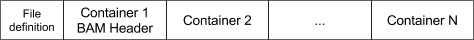
\includegraphics[width=356pt, height=31pt, keepaspectratio=true]{img/CRAMFileFormat2-1-fig001.png}
%%\caption{This should be the caption for \texttt{img/CRAMFileFormat2-1-fig001.png}.}
%%\end{figure}

Pic.1 CRAM file starts with a file definition followed by the BAM header and other 
containers.

Containers consist of one or more blocks. By convention, the BAM header is stored 
in the first container within a single block. This is known as the BAM header block.

%%\begin{figure}[htbp]
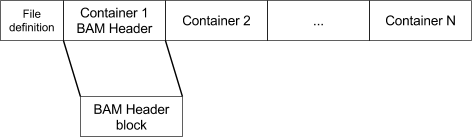
\includegraphics[width=354pt, height=103pt, keepaspectratio=true]{img/CRAMFileFormat2-1-fig002.png}
%%\caption{This should be the caption for \texttt{img/CRAMFileFormat2-1-fig002.png}.}
%%\end{figure}

Pic.2 The BAM header is stored in the first container.

Each container starts with a container header followed by one or more blocks. Each 
block starts with a block header. All data in CRAM is stored within blocks after 
the block header.

%%\begin{figure}[htbp]
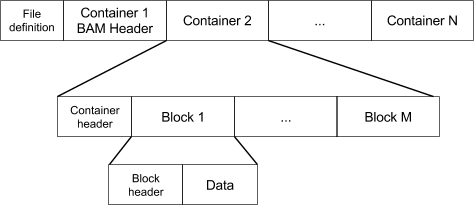
\includegraphics[width=356pt, height=154pt, keepaspectratio=true]{img/CRAMFileFormat2-1-fig003.png}
%%\caption{This should be the caption for \texttt{img/CRAMFileFormat2-1-fig003.png}.}
%%\end{figure}

Pic.3 Container and block structure. All data in CRAM files is stored in blocks.

The first block in each container is the compression header block:

%%\begin{figure}[htbp]
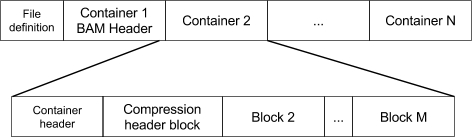
\includegraphics[width=354pt, height=103pt, keepaspectratio=true]{img/CRAMFileFormat2-1-fig004.png}
%%\caption{This should be the caption for \texttt{img/CRAMFileFormat2-1-fig004.png}.}
%%\end{figure}

Pic.4 Compression header is the first block in the container.

The blocks after the compression header are organised logically into slices. One 
slice may contain, for example, a contiguous region of alignment data. Slices begin 
with a slice header block and are followed by one or more data blocks:

%%\begin{figure}[htbp]
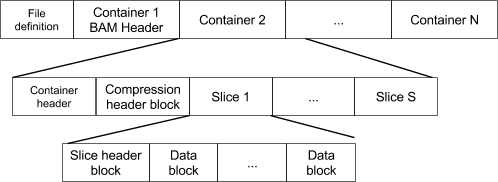
\includegraphics[width=374pt, height=137pt, keepaspectratio=true]{img/CRAMFileFormat2-1-fig005.png}
%%\caption{This should be the caption for \texttt{img/CRAMFileFormat2-1-fig005.png}.}
%%\end{figure}

Pic.5 Containers are logically organised into slices.

Data blocks are divided into core and external data blocks. Each slice must have 
at least one core data block immediately after the slice header block. The core 
data block may be followed by one or more external data blocks.

%%\begin{figure}[htbp]
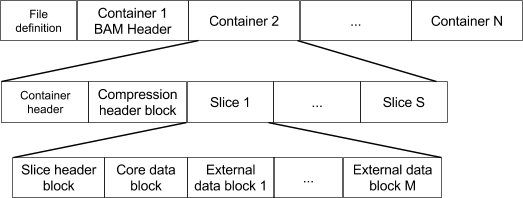
\includegraphics[width=392pt, height=149pt, keepaspectratio=true]{img/CRAMFileFormat2-1-fig006.png}
%%\caption{This should be the caption for \texttt{img/CRAMFileFormat2-1-fig006.png}.}
%%\end{figure}

Pic.5 Data blocks are divided into core and external data blocks. 

\section{\textbf{File definition}}

Each CRAM file starts with a fixed length (26 bytes) definition with the following 
fields:

\begin{tabular}{|l|l|l|}
\hline
\textbf{Data type} & \textbf{Name} & \textbf{Value}\tabularnewline
\hline
byte[4] & format magic number & CRAM (0x43 0x52 0x41 0x4d)\tabularnewline
\hline
unsigned byte & major format number & 3 (0x3)\tabularnewline
\hline
unsigned byte & minor format number & 0 (0x0)\tabularnewline
\hline
byte[20] & file id & CRAM file identifier (e.g. file name or SHA1 checksum)\tabularnewline
\hline
\end{tabular}

Valid CRAM \textit{major}.\textit{minor} version numbers are as follows:

\begin{itemize}
\item[\textit{1.0}]
The original public CRAM release.

\item[\textit{2.0}]
The first CRAM release implemented in both Java and C; tidied up
implementation vs specification differences in \textit{1.0}.

\item[\textit{2.1}]
Gained end of file markers; compatible with \textit{2.0}.

\item[\textit{3.0}]
Additional compression methods; header and data checksums;
improvements for unsorted data.
\end {itemize}

\section{\textbf{Container structure}}

The file definition is followed by one or more containers with the following header 
structure where the container content is stored in the `blocks' field:

\begin{tabular}{|l|>{\raggedright}p{120pt}|>{\raggedright}p{260pt}|}
\hline
\textbf{Data type} & \textbf{Name} & \textbf{Value}
\tabularnewline
\hline
int32 & length & byte size of the container data (blocks)\tabularnewline
\hline
itf8 & reference sequence id & reference sequence identifier  or\linebreak{}
-1 for unmapped reads\linebreak{}
-2 for multiple reference sequences\tabularnewline
\hline
itf8 & starting position on the reference & the alignment start position or\linebreak{}
0 for unmapped reads\tabularnewline
\hline
itf8 & alignment span & the length of the alignment or\linebreak{}
0 for unmapped reads\tabularnewline
\hline
itf8 & number of records & number of records in the container\tabularnewline
\hline
ltf8 & record counter & 1-based sequential index of records in the file/stream.\tabularnewline
\hline
ltf8 & bases & number of read bases\tabularnewline
\hline
itf8 & number of blocks & the number of blocks\tabularnewline
\hline
itf8[ ] & landmarks & Each integer value of this array is a byte offset into the 
blocks byte array. Landmarks are used for random access indexing.\tabularnewline
\hline
int & crc32 & CRC32 hash of the all the preceding bytes in the container.\tabularnewline
\hline
byte[ ] & blocks & The blocks contained within the container.\tabularnewline
\hline
\end{tabular}

\subsection{\textbf{CRAM header in the first container}}

The first container in the CRAM file contains the BAM header in an optionally
compressed block. Only gzip is allowed as compression method for this block. BAM
header is terminated with \textbackslash{}0 byte and any extra bytes in the
block can be used to expand the BAM header. For example when updating @SQ
records additional space may be required for the BAM header. It is recommended
to reserve 50\% more space in the CRAM header block than it is required by the
BAM header.

\section{\textbf{Block structure}}

Containers consist of one or more blocks. Block compression is applied independently 
and in addition to any encodings used to compress data within the block. The block 
have the following header structure with the data stored in the `block data' field:

\begin{tabular}{|l|>{\raggedright}p{120pt}|>{\raggedright}p{260pt}|}
\hline
\textbf{Data type} & \textbf{Name} & \textbf{Value}
\tabularnewline
\hline
byte & method & the block compression method: \linebreak{}
0: raw (none)*\linebreak{}
1: gzip\linebreak{}
2: bzip2\linebreak{}
3: lzma\linebreak{}
4: rans\tabularnewline
\hline
byte & block content type id & the block content type identifier\tabularnewline
\hline
itf8 & block content id & the block content identifier used to associate external 
data blocks with data series\tabularnewline
\hline
itf8 & size in bytes* & size of the block data after applying block compression\tabularnewline
\hline
itf8 & raw size in bytes* & size of the block data before applying block compression\tabularnewline
\hline
byte[ ] & block data & the data stored in the block:\linebreak{}
$\bullet$ bit stream of CRAM records (core data block)\linebreak{}
$\bullet$ byte stream (external data block)\linebreak{}
$\bullet$ additional fields ( header blocks)\tabularnewline
\hline
byte[4] & CRC32 & CRC32 hash value for all preceding bytes in the block\tabularnewline
\hline
\end{tabular}

* Note on raw method: both compressed and raw sizes must be set to the same value.

\subsection{\textbf{Block content types}}

CRAM has the following block content types:

\begin{tabular}{|>{\raggedright}p{143pt}|>{\raggedright}p{45pt}|>{\raggedright}p{116pt}|>{\raggedright}p{114pt}|}
\hline
\textbf{Block content type} & \textbf{Block content type id} & \textbf{Name} & \textbf{Contents}\tabularnewline
\hline
FILE\_HEADER & 0 & BAM header block & BAM header\tabularnewline
\hline
COMPRESSION\_HEADER & 1 & Compression header block & See specific section\tabularnewline
\hline
MAPPED\_SLICE\_HEADER & 2 & Slice header block & See specific section\tabularnewline
\hline
 & 3 &  & reserved\tabularnewline
\hline
EXTERNAL\_DATA & 4 & external data block & data produced by external encodings\tabularnewline
\hline
CORE\_DATA & 5 & core data block & bit stream of all encodings except for external\tabularnewline
\hline
\end{tabular}


\subsection{\textbf{Block content id}}

Block content id is used to distinguish between external blocks in the same slice. 
Each external encoding has an id parameter which must be one of the external block 
content ids. For external blocks the content id is a positive integer. For all 
other blocks content id should be 0. Consequently, all external encodings must 
not use content id less than 1. 

\subsubsection*{Data blocks}

Data is stored in data blocks. There are two types of data blocks: core data blocks 
and external data blocks.The difference between core and external data blocks is 
that core data blocks consist of data series that are compressed using bit encodings 
while the external data blocks are byte compressed. One core data block and any 
number of external data blocks are associated with each slice.

Writing to and reading from core and external data blocks is organised through 
CRAM records. Each data series is associated with an encoding. In case of external 
encoding the block content id is used to identify the block where the data series 
is stored. Please note that external blocks can have multiple data series associated 
with them; in this case the values from these data series will be interleaved. 


\subsection{\textbf{BAM header block}}

The BAM header is stored in a single block within the first container. 

The following constraints apply to the BAM header: 

\begin{itemize}
\item The SQ:MD5 checksum is required unless the reference sequence has been embedded 
into the file.

\item At least one RG record is required.

\item The HD:SO sort order is always POS.
\end{itemize}

\subsection{\textbf{Compression header block}}
\label{subsec:compression-header}

The compression header block consists of 3 parts: preservation map, data series 
encoding map and tag encoding map.

\subsubsection*{Preservation map}

The preservation map contains information about which data was preserved in the 
CRAM file. It is stored as a map with byte[2] keys:

\begin{tabular}{|l|l|>{\raggedright}p{100pt}|>{\raggedright}p{220pt}|}
\hline
\textbf{Key} & \textbf{Value data type} & \textbf{Name} & \textbf{Value}\tabularnewline
\hline
RN & bool & read names included & true if read names are preserved for all reads\tabularnewline
\hline
AP & bool & AP data series delta & true if AP data series is delta, false otherwise\tabularnewline
\hline
RR & bool & reference required & true if reference sequence is required to restore 
the data completely\tabularnewline
\hline
SM & byte[5] & substitution matrix & substitution matrix\tabularnewline
\hline
TD & byte[ ] & tag ids dictionary & a list of lists of tag ids, see tag encoding 
section\tabularnewline
\hline
\end{tabular}

\subsubsection*{Data series encodings}

Each data series has an encoding. These encoding are stored in a map with byte[2] 
keys and are decoded in approximately this order\footnote{The precise order is defined in section~\ref{sec:record}.}:

\begin{threeparttable}[t]
\begin{tabular}{|l|l|>{\raggedright}p{100pt}|>{\raggedright}p{220pt}|}
\hline
\textbf{Key} & \textbf{Value data type} & \textbf{Name} & \textbf{Value}\tabularnewline
\hline
BF & encoding\texttt{<}int\texttt{>} & BAM bit flags & see separate section\tabularnewline
\hline
CF & encoding\texttt{<}int\texttt{>} & CRAM bit flags & see specific section\tabularnewline
\hline
RI & encoding\texttt{<}int\texttt{>} & reference id & record reference id from
the BAM file header\tabularnewline
\hline
RL & encoding\texttt{<}int\texttt{>} & read lengths & read lengths\tabularnewline
\hline
AP & encoding\texttt{<}int\texttt{>} & in-seq positions & 0-based alignment start
delta from previous record *\tabularnewline
\hline
RG & encoding\texttt{<}int\texttt{>} & read groups & read groups. Special value 
`-1' stands for no group.\tabularnewline
\hline
RN\tnote{a} & encoding\texttt{<}byte[ ]\texttt{>} & read names & read names\tabularnewline
\hline
MF & encoding\texttt{<}int\texttt{>} & next mate bit flags & see specific section\tabularnewline
\hline
NS & encoding\texttt{<}int\texttt{>} & next fragment reference sequence id & reference 
sequence ids for the next fragment \tabularnewline
\hline
NP & encoding\texttt{<}int\texttt{>} & next mate alignment start & alignment positions 
for the next fragment\tabularnewline
\hline
TS & encoding\texttt{<}int\texttt{>} & template size & template sizes\tabularnewline
\hline
NF & encoding\texttt{<}int\texttt{>} & distance to next fragment & number of records
to the next fragment\tnote{b}\tabularnewline
\hline
TL\tnote{c} & encoding\texttt{<}int\texttt{>} & tag ids  & list of tag ids, see tag encoding
section\tabularnewline
\hline
FN & encoding\texttt{<}int\texttt{>} & number of read features & number of read
features in each record\tabularnewline
\hline
FC & encoding\texttt{<}byte\texttt{>} & read features codes & see separate section\tabularnewline
\hline
FP & encoding\texttt{<}int\texttt{>} & in-read positions & positions of the read
features\tabularnewline
\hline
DL & encoding\texttt{<}int\texttt{>} & deletion lengths & base-pair deletion lengths\tabularnewline
\hline
BB & encoding\texttt{<}byte[ ]\texttt{>} & stretches of bases & bases\tabularnewline
\hline
QQ & encoding\texttt{<}byte[ ]\texttt{>} & stretches of quality scores & quality scores\tabularnewline
\hline
BS & encoding\texttt{<}byte\texttt{>} & base substitution codes & base substitution
codes\tabularnewline
\hline
IN & encoding\texttt{<}byte[ ]\texttt{>} & insertion & inserted bases\tabularnewline
\hline
RS & encoding\texttt{<}int\texttt{>} & reference skip length & number of skipped 
bases for the `N' read feature\tabularnewline
\hline
PD & encoding\texttt{<}int\texttt{>} & padding & number of padded bases\tabularnewline
\hline
HC & encoding\texttt{<}int\texttt{>} & hard clip & number of hard clipped bases\tabularnewline
\hline
SC & encoding\texttt{<}byte[ ]\texttt{>} & soft clip & soft clipped bases\tabularnewline
\hline
MQ & encoding\texttt{<}int\texttt{>} & mapping qualities & mapping quality scores\tabularnewline
\hline
BA & encoding\texttt{<}byte\texttt{>} & bases & bases\tabularnewline
\hline
QS & encoding\texttt{<}byte\texttt{>} & quality scores & quality scores\tabularnewline
\hline
\end{tabular}

\begin{tablenotes}
\item{a} Note RN this is decoded after MF if the record is detached from the mate and we are attempting to auto-generate read names.
\item{b} The count is reset for each slice so NF can only refer to a record later within this slice.
\item{c} TL is followed by decoding the tag values themselves, in order of appearance in the tag dictionary.
\end{tablenotes}
\end{threeparttable}

\subsubsection*{Tag encodings}
\label{subsubsec:tags}

The tag dictionary (TD) describes the unique combinations of tag id / type that occur on each alignment record.
For example if we search the id / types present in each record and find only two combinations -- X1:i BC:Z SA:Z: and X1:i: BC:Z -- then we have two dictionary entries in the TD map.

Let $L_{i}=\{T_{i0}, T_{i1}, \ldots, T_{ix}\}$ be a list of all tag ids for a record $R_{i}$, where $i$ is the sequential record index and $T_{ij}$ denotes $j$-th tag id in the record.
The list of unique $L_{i}$ is stored as the TD value in the preservation map.
Maintaining the order is not a requirement for encoders (hence ``combinations''), but it is permissible and thus different permutations, each encoded with their own elements in TD, should be supported by the decoder.
Each $L_{i}$ element in TD is assigned a sequential integer number starting with 0.
These integer numbers are referred to by the TL data series.
Using TD, an integer from the TL data series can be mapped back into a list of tag ids.
Thus per alignment record we only need to store tag values and not their ids and types.

The TD is written as a byte array consisting of $L_{i}$ values separated with \textbackslash{}0.
Each $L_{i}$ value is written as a concatenation of 3 byte $T_{ij}$ elements: tag id followed by BAM tag type code (one of A, c, C, s, S, i, I, f, F, Z, H or B, as described in the SAM specification).
For example the TD for tag lists X1:i BC:Z SA:Z and X1:i BC:Z may be encoded as X1CBCZSAZ\textbackslash{}0X1CBCZ\textbackslash{}0, with X1C indicating a 1 byte unsigned value for tag X1.

\subsubsection*{Tag values}

The encodings used for different tags are stored in a map.
The key is 3 bytes formed from the BAM tag id and type code, matching the TD dictionary described above.
Unlike the Data Series Encoding Map, the key is stored in the map as an ITF8 encoded integer, constructed using $(char1<<16) + (char2<<8) + type$.
For example, the 3-byte representation of OQ:Z is \{0x4F, 0x51, 0x5A\} and these bytes are intepreted as the integer key 0x004F515A, leading to an ITF8 byte stream \{0xE0, 0x4F, 0x51, 0x5A\}.

\begin{tabular}{|l|l|l|>{\raggedright}p{160pt}|}
\hline
\textbf{Key} & \textbf{Value data type} & \textbf{Name} & \textbf{Value}
\tabularnewline
\hline
TAG ID 1:TAG TYPE 1 & encoding\texttt{<}byte[ ]\texttt{>} & read tag 1 & tag values
(names and types are available in the data series code)\tabularnewline
\hline
... &  & ... & ...\tabularnewline
\hline
TAG ID N:TAG TYPE N & encoding\texttt{<}byte[ ]\texttt{>} & read tag N & ...\tabularnewline
\hline
\end{tabular}

Note that tag values are encoded as array of bytes. The routines to convert tag 
values into byte array and back are the same as in BAM with the exception of value 
type being captured in the tag key rather in the value.
Hence consuming 1 byte for types `C' and `c', 2 bytes for types `S' and `s', 4 bytes for types `I', `i' and `f', and a variable number of bytes for types `H', `Z' and `B'.

\subsection{\textbf{Slice header block}}

The slice header block is never compressed (block method=raw). For reference mapped 
reads the slice header also defines the reference sequence context of the data 
blocks associated with the slice. Mapped and unmapped reads can be stored within 
the same slice similarly to BAM file. Slices with unsorted reads must not contain 
any other types of reads.

The slice header block contains the following fields.

\begin{tabular}{|l|l|>{\raggedright}p{200pt}|}
\hline
\textbf{Data type} & \textbf{Name} & \textbf{Value}\tabularnewline
\hline
itf8 & reference sequence id & reference sequence identifier or -1 for unmapped 
or unsorted reads\tabularnewline
\hline
itf8 & alignment start & the alignment start position or -1 for unmapped or unsorted 
reads\tabularnewline
\hline
itf8 & alignment span & the length of the alignment or 0 for unmapped or unsorted 
reads\tabularnewline
\hline
itf8 & number of records & the number of records in the slice\tabularnewline
\hline
ltf8 & record counter & 1-based sequential index of records in the file/stream\tabularnewline
\hline
itf8 & number of blocks & the number of blocks in the slice\tabularnewline
\hline
itf8[ ] & block content ids & block content ids of the blocks in the slice\tabularnewline
\hline
itf8 & embedded reference bases block content id & block content id for the embedded 
reference sequence bases or -1 for none\tabularnewline
\hline
byte[16] & reference md5 & MD5 checksum of the reference bases within the slice 
boundaries or 16 \textbackslash{}0 bytes for unmapped or unsorted reads\tabularnewline
\hline
byte[] & optional tags & a series of tag,type,value tuples encoded as
per BAM auxiliary fields.\tabularnewline
\hline
\end{tabular}

The optional tags are encoded in the same manner as BAM tags.  I.e. a
series of binary encoded tags concatenated together where each tag
consists of a 2 byte key (matching [A-Za-z][A-Za-z0-9]) followed by a
1 byte type ([AfZHcCsSiIB]) followed by a string of bytes in a format
defined by the type.

Tags starting in a capital letter are reserved while lowercase ones or
those starting with X, Y or Z are user definable.  Any tag not
understood by a decoder should be skipped over without producing an
error.

At present no tags are defined.

% Details omitted until we fully work through all the corner cases,
% such as seq/qual of *.
%
% Reserved tags are defined as follows:
% 
% \begin{tabular}{|l|l|>{\raggedright}p{325pt}|}
% \hline
% \textbf{Tag type} & \textbf{BAM format} & \textbf{Meaning}\tabularnewline
% \hline
% BD & i & Sum over all reads of the CRC32 hash of sequence base.  This
% may be used to validate round-trips in and out of CRAM.
% calls\tabularnewline
% \hline
% SD & i & Sum over all reads of the CRC32 hash of quality scores. (If
% the quality string is ``*'' in SAM then the hash is of the BAM encoded
% version - a string of bytes with value 255.)\tabularnewline
% \hline
% \end{tabular}


\subsection{\textbf{Core data block}}

A core data block is a bit stream (most significant bit first) consisting of one 
or more CRAM records. Please note that one byte could hold more then one CRAM record 
as a minimal CRAM record could be just a few bits long. The core data block has 
the following fields:

\begin{tabular}{|l|>{\raggedright}p{120pt}|>{\raggedright}p{260pt}|}
\hline
\textbf{Data type} & \textbf{Name} & \textbf{Value}
\tabularnewline
\hline
bit[ ] & CRAM record 1 & The first CRAM record\tabularnewline
\hline
... & ... & ...\tabularnewline
\hline
bit[ ] & CRAM record N & The Nth CRAM record \tabularnewline
\hline
\end{tabular}

\subsection{\textbf{External data block}}

Relationship between core data block and external data blocks is shown in the following 
picture: 

%%\begin{figure}[htbp]
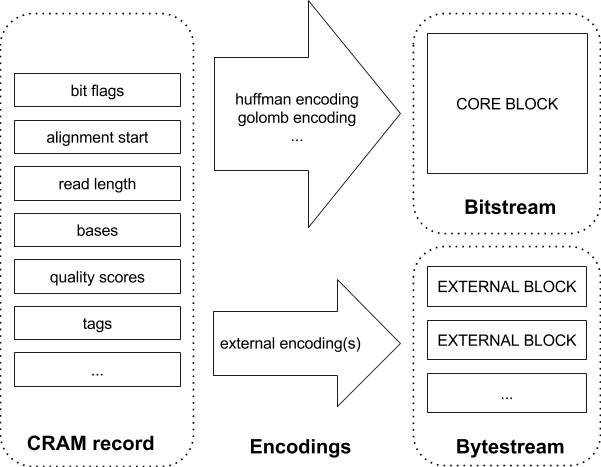
\includegraphics[width=451pt, height=350pt, keepaspectratio=true]{img/CRAMFileFormat2-1-fig007.png}
%%\caption{This should be the caption for \texttt{img/CRAMFileFormat2-1-fig007.png}.}
%%\end{figure}

Pic.3 Relationship between core data block and external data blocks.

The picture shows how a CRAM record (on the left) is partially written to core 
data block while the other fields are stored in two external data blocks. The specific 
encodings are presented only for demonstration purposes, the main point here is 
to distinguish between bit encodings whose output is always stored in core data 
block and the external encoding which simply stored the bytes into external data 
blocks.

\section{\textbf{End of file marker}}

A special container is used to mark the end of a file or stream. It is required in version 3 or later. The idea is to provide an easy and a quick way to detect that a CRAM file or stream is complete. The marker is basically an empty container with ref seq id set to -1 (unaligned) and alignment 
start set to 4542278.

Here is a complete content of the EOF container explained in detail:

\begin{tabular}{|l|l|>{\raggedright}p{150pt}|>{\raggedright}p{180pt}|}
\hline
\textbf{hex bytes} & \textbf{data type} & \textbf{decimal value} & \textbf{field 
name}\tabularnewline
\hline
\multicolumn{4}{|l|}{\textit{Container header}}\tabularnewline
\hline
0f 00 00 00 & integer & 15 & size of blocks data\tabularnewline
\hline
ff ff ff ff 0f & itf8 & -1 & ref seq id\tabularnewline
\hline
e0 45 4f 46 & itf8 & 4542278 & alignment start\tabularnewline
\hline
00 & itf8 & 0 & alignment span\tabularnewline
\hline
00 & itf8 & 0 & number of records\tabularnewline
\hline
00 & itf8 & 0 & global record counter\tabularnewline
\hline
00 & itf8 & 0 & bases\tabularnewline
\hline
01 & itf8 & 1 & block count\tabularnewline
\hline
00 & array & 0 & landmarks\tabularnewline
\hline
05 bd d9 4f & integer & 1339669765 & container header CRC32\tabularnewline
\hline
\multicolumn{4}{|l|}{\textit{Compression header block}}\tabularnewline
\hline
00 & byte & 0 (RAW) & compression method\tabularnewline
\hline
01 & byte & 1 (COMPRESSION\_HEADER) & block content type\tabularnewline
\hline
00 & itf8 & 0 & block content id\tabularnewline
\hline
06 & itf8 & 6 & compressed size\tabularnewline
\hline
06 & itf8 & 6 & uncompressed size\tabularnewline
\hline
\multicolumn{4}{|l|}{\textit{Compression header}}\tabularnewline
\hline
01 & itf8 & 1 & preservation map byte size\tabularnewline
\hline
00 & itf8 & 0 & preservation map size\tabularnewline
\hline
01 & itf8 & 1 & encoding map byte size\tabularnewline
\hline
00 & itf8 & 0 & encoding map size\tabularnewline
\hline
01 & itf8 & 1 & tag encoding byte size\tabularnewline
\hline
00 & itf8 & 0 & tag encoding map size\tabularnewline
\hline
ee 63 01 4b & integer & 1258382318 & block CRC32\tabularnewline
\hline
\end{tabular}

When compiled together the EOF marker is 38 bytes long and in hex representation 
is:

0f 00 00 00 ff ff ff ff 0f e0 45 4f 46 00 00 00 00 01 00 05 bd d9 4f 00 01 00 06 06 01 00 01 00 01 00 ee 63 01 4b

\section{\textbf{Record structure}}
\label{sec:record}

CRAM record is based on the SAM record but has additional features allowing for 
more efficient data storage.  In contrast to BAM record CRAM record uses bits as 
well as bytes for data storage. This way, for example, various coding techniques 
which output variable length binary codes can be used directly in CRAM. On the 
other hand, data series that do not require binary coding can be stored separately 
in external blocks with some other compression applied to them independently.

As CRAM data series may be interleaved within the same blocks\footnote{Interleaving can sometimes provide better compression, however it also adds dependency between types of data meaning it is not possible to selectively decode one data series if it co-locates with another data series in the same block.} understanding the order in which CRAM data series must be decoded is vital.

The overall flowchart is below, with more detailed description in the subsequent sections.

\algnewcommand\algorithmicto{\text{ \textbf{to} }}

\subsection{\textbf{CRAM record}}

Both mapped and unmapped reads start with the following fields. Please note that 
the data series type refers to the logical data type and the data series name corresponds 
to the data series encoding map.

\begin{tabular}{|>{\raggedright}p{70pt}|>{\raggedright}p{75pt}|>{\raggedright}p{90pt}|>{\raggedright}p{171pt}|}
\hline
\textbf{Data series type} & \textbf{Data series name} & \textbf{Field} & \textbf{Description}\tabularnewline
\hline
int & BF & BAM bit flags & see BAM bit flags below\tabularnewline
\hline
int & CF & CRAM bit flags & see CRAM bit flags below\tabularnewline
\hline
- & - & Positional data & See section \ref{subsec:positions}\tabularnewline
\hline
- & - & Read names & See section \ref{subsec:names}\tabularnewline
\hline
- & - & Mate records & See section \ref{subsec:mate}\tabularnewline
\hline
- & - & Auxiliary tags & See section \ref{subsec:tags}\tabularnewline
\hline
- & - & Sequences & See sections \ref{subsec:mapped} and \ref{subsec:unmapped}\tabularnewline
\hline
\end{tabular}

\subsubsection*{\textbf{BAM bit flags (BF data series)}}

The following flags are duplicated from the SAM and BAM specification, with identical meaning.
Note however some of these flags can be derived during decode, so may be omitted in the CRAM file and the bits computed based on both reads of a pair-end library residing within the same slice.

\begin{threeparttable}[t]
\begin{tabular}{|>{\raggedright}p{144pt}|>{\raggedright}p{144pt}|>{\raggedright}p{144pt}|}
\hline
\textbf{Bit flag} & \textbf{Comment} & \textbf{Description}\tabularnewline
\hline
0x1 &  & template having multiple segments in sequencing\tabularnewline
\hline
0x2 &  & each segment properly aligned according to the aligner\tabularnewline
\hline
0x4 &  & segment unmapped\tnote{a}\tabularnewline
\hline
0x8 & calculated\tnote{b}\ \ or stored in the mate's info & next segment in template unmapped\tabularnewline
\hline
0x10 &  & SEQ being reverse complemented\tabularnewline
\hline
0x20 & calculated\tnote{b}\ \ or stored in the mate's info & SEQ of the next segment in the
template being reversed\tabularnewline
\hline
0x40 &  & the first segment in the template\tnote{c}\tabularnewline
\hline
0x80 &  & the last segment in the template\tnote{c}\tabularnewline
\hline
0x100 &  & secondary alignment\tabularnewline
\hline
0x200 &  & not passing quality controls\tabularnewline
\hline
0x400 &  & PCT or optical duplicate\tabularnewline
\hline
0x800 &  & Supplementary alignment\tabularnewline
\hline
\end{tabular}
\begin{tablenotes}
\item[a] Bit 0x4 is the only reliable place to tell whether the read is unmapped.  If 0x4 is set, no assumptions may be made about bits 0x2, 0x100 and 0x800.
\item[b] For segments within the same slice.
\item[c] Bits 0x40 and 0x80 reflect the read ordering within each template inherent in the sequencing technology used, which may be independent from the actual mapping orientation.
If 0x40 and 0x80 are both set, the read is part of a linear template (one where the template sequence is expected to be in a linear order), but it is neither the first nor the last read.
If both 0x40 and 0x80 are unset, the index of the read in the template is unknown.
This may happen for a non-linear template (such as one constructed by stitching together other templates) or when this information is lost during data processing.
\end{tablenotes}
\end{threeparttable}

\subsubsection*{\textbf{CRAM bit flags (CF data series)}}

The CRAM bit flags (also known as compression bit flags) expressed as an integer represent the CF data series. 
The following compression flags are defined for each CRAM read record:

\begin{tabular}{|>{\raggedright}p{39pt}|>{\raggedright}p{150pt}|>{\raggedright}p{242pt}|}
\hline
\textbf{Bit flag} & \textbf{Name} & \textbf{Description}\tabularnewline
\hline
0x1 & quality scores stored as array & quality scores can be stored as read features
or as an array similar to read bases.\tabularnewline
\hline
0x2 & detached & mate information is stored verbatim (e.g. because the pair spans multiple slices or the fields differ to the CRAM computed method)\tabularnewline
\hline
0x4 & has mate downstream & tells if the next segment should be expected further
in the stream\tabularnewline
\hline
0x8 & decode sequence as ``*'' & informs the decoder that the sequence
is unknown and that any encoded reference differences are present only to
recreate the CIGAR string.\tabularnewline
\hline
\end{tabular}


The following pseudocode describes the general process of decoding an entire CRAM record.
The sequence data itself is in one of two encoding formats depending on whether the record is aligned (mapped).

\subsubsection*{\textbf{Decode pseudocode}}
\newlength{\maxwidth}
\newcommand{\algalign}[2] % #1 = text to left, #2 = text to right
{\makebox[\maxwidth][l]{$#1{}$}${}#2$}

\begin{algorithmic}[1]
\Procedure{DecodeRecord}{}
\settowidth{\maxwidth}{CRAM\_flags\quad}
\State \algalign{BAM\_flags}{\gets}  \Call{ReadItem}{BF, Integer}
\State \algalign{CRAM\_flags}{\gets} \Call{ReadItem}{CF, Integer}
\State \Call{DecodePositions}{}\Comment{See section \ref{subsec:positions}}
\State \Call{DecodeNames}{}\Comment{See section \ref{subsec:names}}
\State \Call{DecodeMateData}{}\Comment{See section \ref{subsec:mate}}
\State \Call{DecodeTagData}{}\Comment{See section \ref{subsec:tags}}
\Statex

\If{$(BF$ AND $4) \ne 0$}\Comment{Unmapped flag}
  \State \Call{DecodeMappedRead}{}\Comment{See section \ref{subsec:mapped}}
\Else
  \State \Call{DecodeUnmappedRead}{}\Comment{See section \ref{subsec:unmapped}}
\EndIf
\EndProcedure
\end{algorithmic}

\subsection{\textbf{CRAM positional data}}
\label{subsec:positions}

Following the bit-wise BAM and CRAM flags, CRAM encodes positional related data including reference, alignment positions and length, and read-group.
Positional data is stored for both mapped and unmapped sequences, as unmapped data may still be ``placed'' at a specific location in the genome (without being aligned).
Typically this is done to keep a sequence pair (paired-end or mate-pair sequencing libraries) together when one of the pair aligns and the other does not.

The AP data series is delta encoded for reads mapped to a position-sorted slice containing data from a single reference, and as a normal integer value in all other cases.

\begin{tabular}{|>{\raggedright}p{70pt}|>{\raggedright}p{75pt}|>{\raggedright}p{90pt}|>{\raggedright}p{171pt}|}
\hline
\textbf{Data series type} & \textbf{Data series name} & \textbf{Field} & \textbf{Description}\tabularnewline
\hline
int & RI & ref id & reference sequence id (only present in multiref slices)\tabularnewline
\hline
int & RL & read length & the length of the read\tabularnewline
\hline
int & AP & alignment start & the alignment start position\tabularnewline
\hline
int & RG & read group & the read group identifier expressed as the N\textsuperscript{th} record in the header, starting from 0 with -1 for no group\tabularnewline
\hline
\end{tabular}

\vskip 20pt
\begin{algorithmic}[1]
\Procedure{DecodePositions}{}
\If{$slice\_header.reference\_sequence\_id = -2$}
  \State $reference\_id\gets$ \Call{ReadItem}{RI, Integer}
\Else
  \State $reference\_id\gets slice\_header.reference\_sequence\_id$
\EndIf
\State $read\_length \gets$ \Call{ReadItem}{RL, Integer}
\If{$container\_pmap.AP\_delta \ne 0$}
    \State Initialise $last\_position$ to 0 if first record in slice
    \State $alignment\_position \gets$ \Call{ReadItem}{AP, Integer} + $last\_position$
    \State $last\_position \gets alignment\_position$
\Else
    \State $alignment\_position \gets$ \Call{ReadItem}{AP, Integer}
\EndIf
\State $read\_group \gets$ \Call{ReadItem}{RG, Integer}
\EndProcedure
\end{algorithmic}

\subsection{Read names (RN data series)}
\label{subsec:names}

Read names can be preserved in the CRAM format, but this is optional and is governed by the \texttt{RN} preservation map key in the container compression header. See section \ref{subsec:compression-header}.
When read names are not preserved the CRAM decoder should generate names, typically based on the file name and a numeric ID of the read using the record counter field of the slice header block.
Note read names may still be preserved even when the \texttt{RN} compression header key indicates otherwise, such as where a read is part of a read-pair and the pair spans multiple slices.
In this situation the record will be marked as detached (see the CF data series) and the mate data below (section \ref{subsec:mate}) will contain the read name.

\begin{tabular}{|>{\raggedright}p{70pt}|>{\raggedright}p{75pt}|>{\raggedright}p{90pt}|>{\raggedright}p{171pt}|}
\hline
\textbf{Data series type} & \textbf{Data series name} & \textbf{Field} & \textbf{Description}\tabularnewline
\hline
byte[] & RN & read names & read names\tabularnewline
\hline
\end{tabular}

\vskip 20pt
\begin{algorithmic}[1]
\Procedure{DecodeNames}{}
\If{$container\_pmap.read\_names\_included = 1$}
  \State $read\_name \gets$ \Call{ReadItem}{RN, Byte[]}
\Else
  \State $read\_name \gets$ \Call{GenerateName}{}
\EndIf
\Statex
\EndProcedure
\end{algorithmic}

\subsection{\textbf{Mate record}}
\label{subsec:mate}

There are two ways in which mate information can be preserved in CRAM: number of records downstream (distance, within this slice) to the next fragment in the template and a special mate record if the next fragment is not in the current slice.
In the latter case the record is labelled as ``detached'', see the CF data series.

For mates within the slice only the distance is captured, and only for the first record.  The mate has neither detached nor downstream flags set in the CF data series.

\begin{tabular}{|>{\raggedright}p{68pt}|>{\raggedright}p{115pt}|>{\raggedright}p{228pt}|}
\hline
\textbf{Data series type} & \textbf{Data series name} & \textbf{Description}\tabularnewline
\hline
int & NF & the number of records to the next fragment\tabularnewline
\hline
\end{tabular}

In the above case, the NS (mate reference name), NP (mate position) and TS (template size) fields for both records should be derived once the mate has also been decoded.
Mate reference name and position are obvious and simply copied from the mate.
The template size is computed using the method described in the SAM specification; the inclusive distance from the leftmost to rightmost mapped bases with the sign being positive for the leftmost record and negative for the rightmost record.

If the next fragment is not found within this slice then the following structure is included into the CRAM record.
Note there are cases where read-pairs within the same slice may be marked as detached and use this structure, such as to store mate-pair information that does not match the algorithm used by CRAM for computing the mate data on-the-fly.

\begin{tabular}{|>{\raggedright}p{66pt}|>{\raggedright}p{117pt}|>{\raggedright}p{228pt}|}
\hline
\textbf{Data series type} & \textbf{Data series name} & \textbf{Description}\tabularnewline
\hline
int & MF & next mate bit flags, see table below\tabularnewline
\hline
byte[ ] & RN & the read name (if and only if not known already)\tabularnewline
\hline
int & NS & mate reference sequence identifier \tabularnewline
\hline
int & NP & mate alignment start position \tabularnewline
\hline
int & TS & the size of the template (insert size)\tabularnewline
\hline
\end{tabular}

\subsubsection*{Next mate bit flags (MF data series)}

The next mate bit flags expressed as an integer represent the MF data series.
These represent the missing bits we excluded from the BF data series (when compared to the full SAM/BAM flags).
The following bit flags are defined:

\begin{tabular}{|>{\raggedright}p{47pt}|>{\raggedright}p{134pt}|>{\raggedright}p{250pt}|}
\hline
\textbf{Bit flag} & \textbf{Name} & \textbf{Description}\tabularnewline
\hline
0x1 & mate negative strand bit & the bit is set if the mate is on the negative
strand\tabularnewline
\hline
0x2 & mate mapped bit & the bit is set if the mate is mapped\tabularnewline
\hline
\end{tabular}


\subsubsection*{\textbf{Decode mate pseudocode}}

In the following pseudocode we are assuming the current record is $this$ and its mate is $next\_frag$.

\begin{algorithmic}[1]
\Procedure{DecodeMateData}{}
\If{$CF$ AND $2$}\Comment{Detached from mate}
  \State $mate\_flags\gets $ \Call{ReadItem}{MF,Integer}
  \If{$mate\_flags$ AND 1}
    \State $bam\_flags\gets bam\_flags$\ OR\ 0x20\Comment{Mate is reverse-complemented}
  \EndIf
  \If{$mate\_flags$ AND 2}
    \State $bam\_flags\gets bam\_flags$\ OR\ 0x08\Comment{Mate is unmapped}
  \EndIf
  \If{$container\_pmap.read\_names\_included \ne 1$}
    \State $read\_name \gets$ \Call{ReadItem}{RN, Byte[]}
  \EndIf
\settowidth{\maxwidth}{mate\_position\ }
\State \algalign{mate\_ref\_id}{\gets}  \Call{ReadItem}{NS, Integer}
\State \algalign{mate\_position}{\gets} \Call{ReadItem}{NP, Integer}
\State \algalign{template\_size}{\gets} \Call{ReadItem}{TS, Integer}
\ElsIf{$CF$ AND $4$}\Comment{Mate is downstream}
  \If{$next\_frag.bam\_flags$ AND 0x10}
    \State $this.bam\_flags \gets this.bam\_flags$\ OR\ 0x20\Comment{next segment reverse complemented}
  \EndIf
  \If{$next\_frag.bam\_flags$ AND 0x04}
    \State $this.bam\_flags \gets this.bam\_flags$\ OR\ 0x08\Comment{next segment unmapped}
  \EndIf
  \State $next\_frag\gets$ \Call{ReadItem}{NF,Integer}
  \State Resolve $mate\_ref\_id$ for $this$ record and $this+next\_frag$ once both have been decoded
  \State Resolve $mate\_position$ for $this$ record and $this+next\_frag$ once both have been decoded
  \State Find leftmost and rightmost mapped coordinate in records $this$ and $this+next\_frag$.
  \State For leftmost of $this$ and $this+next\_frag$ record: $template\_size\gets rightmost-leftmost+1$
  \State For rightmost of $this$ and $this+next\_frag$ record: $template\_size\gets -(rightmost-leftmost+1)$
\EndIf
\EndProcedure
\end{algorithmic}

Note as with the SAM specification a template may be permitted to have more than two alignment records.
In this case the ``mate'' for each record is considered to be the next record, with the mate for the last record being the first to form a circular list.
The above algorithm is a simplification that does not deal with this scenario.
The full method needs to observe when record $this+NF$ is also labelled as having an additional mate downstream.
One recommended approach is to resolve the mate information in a second pass, once the entire slice has been decoded.
The final segment in the mate chain needs to set $bam\_flags$ fields 0x20 and 0x08 accordingly based on the first segment.
This is also not listed in the above algorithm, for brevity.

\subsection{Auxiliary tags}
\label{subsec:tags}

Tags are encoded using a tag line (TL data series) integer into the tag dictionary (TD field in the compression header preservation map, see section \ref{subsec:compression-header}).
See section \ref{subsubsec:tags} for a more detailed description of this process.

\begin{tabular}{|>{\raggedright}p{70pt}|>{\raggedright}p{75pt}|>{\raggedright}p{90pt}|>{\raggedright}p{200pt}|}
\hline
\textbf{Data series type} & \textbf{Data series name} & \textbf{Field} & \textbf{Description}\tabularnewline
\hline
int & TL & tag line & an index into the tag dictionary (TD)\tabularnewline
\hline
* & ??? & tag name/type & 3 character key (2 tag identifier and 1 tag type), as specified by the tag dictionary\tabularnewline
\hline
\end{tabular}

\vskip 20pt
\begin{algorithmic}[1]
\Procedure{DecodeTagData}{}
\State $tag\_line\gets$ \Call{ReadItem}{TL,Integer}
\ForAll {$ele \in container\_pmap.tag\_dict(tag\_line)$}
  \State $name\gets$ first two characters of $ele$
  \State $tag(type)\gets$ last character of $ele$
  \State $tag(name)\gets$ \Call{ReadItem}{$ele$, Byte[]}
\EndFor
\EndProcedure
\end{algorithmic}

In the above procedure, $name$ is a two letter tag name and $type$ is one of the permitted types documented in the SAM/BAM specification.
Type is \texttt{c} (signed 8-bit integer), \texttt{C} (unsigned 8-bit integer), \texttt{s} (signed 16-bit integer), \texttt{S} (unsigned 16-bit integer), \texttt{i} (signed 32-bit integer), \texttt{I} (unsigned 32-bit integer), \texttt{f} (32-bit float), \texttt{Z} (nul-terminated string), \texttt{H} (nul-terminated string of hex digits) and \texttt{B} (binary data in array format with the first byte being one of c,C,s,S,i,I,f using the meaning above, a 32-bit integer for the number of array elements, followed by array data encoded using the specified format).  All integers are little endian encoded.

For example a SAM tag \texttt{MQ:i} has name \texttt{MQ} and type \texttt{i} and will be decoded using one of MQc, MQC, MQs, MQS, MQi and MQI data series depending on size and sign of the integer value.

\subsection{\textbf{Mapped reads}}
\label{subsec:mapped}

\subsubsection*{\textbf{Read feature records}}
\label{subsec:features}

Read features are used to store read details that are expressed using read coordinates 
(e.g. base differences respective to the reference sequence). The read feature 
records start with the number of read features followed by the read features themselves.
Finally the single mapping quality and per-base quality scores are stored.

\begin{threeparttable}[t]
\begin{tabular}{|>{\raggedright}p{88pt}|>{\raggedright}p{83pt}|>{\raggedright}p{85pt}|>{\raggedright}p{180pt}|}
\hline
\textbf{Data series type} & \textbf{Data series name} & \textbf{Field} & \textbf{Description}\tabularnewline
\hline
int & FN & number of read features & the number of read features\tabularnewline
\hline
int & FP & in-read-position\tnote{a} & position of the read feature\tabularnewline 
\hline
byte & FC & read feature code\tnote{a} & See feature codes below\tabularnewline
\hline
* & * & read feature data\tnote{a} & See feature codes below\tabularnewline
\hline
int & MQ & mapping qualities & mapping quality score\tabularnewline
\hline
byte[read length] & QS & quality scores & the base qualities, if preserved\tabularnewline
\hline
\end{tabular}
\begin{tablenotes}
\item[a] Repeated FN times, once for each read feature.
\end{tablenotes}
\end{threeparttable}

\subsubsection*{Read feature codes}

Each feature code has its own associated data series containing further information specific to that feature.
The following codes are used to distinguish variations in read coordinates:

\begin{tabular}{|>{\raggedright}p{91pt}|>{\raggedright}p{45pt}|>{\raggedright}p{72pt}|>{\raggedright}p{66pt}|>{\raggedright}p{132pt}|}
\hline
\textbf{Feature code} & \textbf{Id} & \textbf{Data series type} & \textbf{Data 
series name} & \textbf{Description}\tabularnewline
\hline
Bases & b (0x62) & byte[ ] & BB & a stretch of bases\tabularnewline
\hline
Scores & q (0x71) & byte[ ] & QQ & a stretch of scores\tabularnewline
\hline
% Neither C nor Java implementations generator nor can decode the 'A'
% feature code, but if they did they'd be BB/QQ and not BA/QS.  Best
% to omit it from published spec for now?
%
% Bases and scores & A (0x41) & byte[ ],byte[ ] & BB,QQ & A a stretch of bases and
% quality scores score\tabularnewline
% \hline
Read base & B (0x42) & byte,byte & BA,QS & A base and associated quality score\tabularnewline
\hline
Substitution & X (0x58) & byte & BS & base substitution codes, SAM operators X, 
M and =\tabularnewline
\hline
Insertion & I (0x49) & byte[ ] & IN & inserted bases, SAM operator I\tabularnewline
\hline
Deletion & D (0x44) & int & DL & number of deleted bases, SAM operator D\tabularnewline
\hline
Insert base & i (0x69) & byte & BA & single inserted base, SAM operator I\tabularnewline
\hline
Quality score & Q (0x51) & byte & QS & single quality score\tabularnewline
\hline
Reference skip & N (0x4E) & int & RS & number of skipped bases, SAM operator N\tabularnewline
\hline
Soft clip & S (0x53) & byte[ ] & SC & soft clipped bases, SAM operator S\tabularnewline
\hline
Padding & P (0x50) & int & PD & number of padded bases, SAM operator P\tabularnewline
\hline
Hard clip & H (0x48) & int & HC & number of hard clipped bases, SAM operator H\tabularnewline
\hline
\end{tabular}

\subsubsection*{Base substitution codes (BS data series)}

A base substitution is defined as a change from one nucleotide base (reference 
base) to another (read base) including N as an unknown or missing base. There are 
5 possible bases ACGTN, 4 possible substitutions for each base and 20 substitutions 
in total. Substitutions for the same reference base are assigned integer codes 
from 0 to 3 inclusive. To restore a base one would need to know its substitution 
code and the reference base. 

A base substitution matrix assigns integer codes to all possible substitutions. 

Substitution matrix is written as follows. Substitutions for a given reference 
base are sorted by their frequencies in descending order then assigned numbers 
from 0 to 3. Same-frequency ties are broken using alphabetical order. For example, 
let us assume the following substitution frequencies for base A: 

AC: 15\%

AG: 25\%

AT: 55\%

AN: 5\%

Then the substitution codes are: 

AC: 2

AG: 1

AT: 0

AN: 3

and they are written as a single byte, 10 01 00 11 = 147 decimal or 0x93 in this 
case. The whole substitution matrix is written as 5 bytes, one for each reference 
base in the alphabetical order: A, C, G, T and N.

Note: the last two bits of each substitution code are redundant but still required 
to simplify the reading. 

\subsubsection*{Decode mapped read pseudocode}

\begin{algorithmic}[1]
\Procedure{DecodeMappedRead}{}
  \State $feature\_number\gets$ \Call{ReadItem}{FN, Integer} 
  \For{$i\gets 1 \algorithmicto feature\_number$}
    \State \Call{DecodeFeature}{}
  \EndFor
  \State $mapping\_quality\gets$ \Call{ReadItem}{MQ, Integer} 
  \If{$container\_pmap.preserve\_quality\_scores$}
    \For{$i\gets 1 \algorithmicto read\_length$}
      \State $quality\_score\gets$ \Call{ReadItem}{QS, Integer} 
    \EndFor
  \EndIf
\EndProcedure
\Statex
\Procedure{DecodeFeature}{}
    \settowidth{\maxwidth}{feature\_position\ }
    \State \algalign{feature\_code}{\gets}       \Call{ReadItem}{FC, Integer} 
    \State \algalign{feature\_position}{\gets}   \Call{ReadItem}{FP, Integer} 
    \settowidth{\maxwidth}{substitution\_code\ }
    \If{$feature\_code = $`B'}
      \State \algalign{base}{\gets}              \Call{ReadItem}{BA, Byte}
      \State \algalign{quality\_score}{\gets}    \Call{ReadItem}{QS, Byte}
    \ElsIf{$feature\_code = $`X'}
      \State \algalign{substitution\_code}{\gets} \Call{ReadItem}{BS, Byte}
    \ElsIf{$feature\_code = $`I'}
      \State \algalign{inserted\_bases}{\gets}   \Call{ReadItem}{IN, Byte[]}
    \ElsIf{$feature\_code = $`S'}
      \State \algalign{softclip\_bases}{\gets}   \Call{ReadItem}{SC, Byte[]}
    \ElsIf{$feature\_code = $`H'}
      \State \algalign{hardclip\_length}{\gets}  \Call{ReadItem}{HC, Integer}
    \ElsIf{$feature\_code = $`P'}
      \State \algalign{pad\_length}{\gets}       \Call{ReadItem}{PD, Integer}
    \ElsIf{$feature\_code = $`D'}
      \State \algalign{deletion\_length}{\gets}  \Call{ReadItem}{DL, Integer}
    \ElsIf{$feature\_code = $`N'}
      \State \algalign{ref\_skip\_length}{\gets} \Call{ReadItem}{RS, Integer}
    \ElsIf{$feature\_code = $`i'}
      \State \algalign{base}{\gets}              \Call{ReadItem}{BA, Byte}
    \ElsIf{$feature\_code = $`b'}
      \State \algalign{bases}{\gets}             \Call{ReadItem}{BB, Byte[]}
    \ElsIf{$feature\_code = $`q'}
      \State \algalign{quality\_scores}{\gets}   \Call{ReadItem}{QQ, Byte[]}
    \ElsIf{$feature\_code = $`Q'}
      \State \algalign{quality\_score}{\gets}    \Call{ReadItem}{QS, Byte}
    \EndIf
\EndProcedure
\end{algorithmic}

\subsection{\textbf{Unmapped reads}}
\label{subsec:unmapped}

The CRAM record structure for unmapped reads has the following additional fields:

\begin{tabular}{|>{\raggedright}p{88pt}|>{\raggedright}p{83pt}|>{\raggedright}p{85pt}|>{\raggedright}p{180pt}|}
\hline
\textbf{Data series type} & \textbf{Data series name} & \textbf{Field} & \textbf{Description}\tabularnewline
\hline
byte[read length] & BA & bases & the read bases\tabularnewline
\hline
byte[read length] & QS & quality scores & the base qualities, if preserved\tabularnewline
\hline
\end{tabular}

\vskip20pt
\begin{algorithmic}[1]
\Procedure{DecodeUnmappedRead}{}
  \For{$i\gets 1 \algorithmicto read\_length$}
    \State $base\gets$ \Call{ReadItem}{BA, Byte}
  \EndFor
  \If{$container\_pmap.preserve\_quality\_scores$}
    \For{$i\gets 1 \algorithmicto read\_length$}
      \State $quality\_score\gets$ \Call{ReadItem}{QS, Byte}
    \EndFor
  \EndIf
\EndProcedure
\end{algorithmic}

\section{\textbf{Reference sequences}}

CRAM format is natively based upon usage of reference sequences even though in 
some cases they are not required. In contrast to BAM format CRAM format has strict 
rules about reference sequences. 

\begin{enumerate}
\item M5 (sequence MD5 checksum) field of @SQ sequence record in the BAM header is 
required and UR (URI for the sequence fasta optionally gzipped file) field is strongly 
advised. The rule for calculating MD5 is to remove any non-base symbols (like \textbackslash{}n, 
sequence name or length and spaces) and upper case the rest. Here are some examples: 

\texttt{> samtools faidx human\_g1k\_v37.fasta 1 \textbar{} grep -v '\textasciicircum{}>' \textbar{} tr -d '\textbackslash{}n' \textbar{} tr a-z A-Z \textbar{} md5sum -\\
1b22b98cdeb4a9304cb5d48026a85128  -}

\texttt{> samtools faidx human\_g1k\_v37.fasta 1:10-20 \textbar{}grep -v '\textasciicircum{}\texttt{>}' \textbar{}tr -d '\textbackslash{}n' \textbar{}tr a-z A-Z \textbar{}md5sum -\\
0f2a4865e3952676ffad2c3671f14057  -}

Please note that the latter calculates the checksum for 11 bases from position 
10 (inclusive) to 20 (inclusive) and the bases are counted 1-based, so the first 
base position is 1. 

\item All CRAM reader implementations are expected to check for reference MD5 checksums 
and report any missing or mismatching entries. Consequently, all writer implementations 
are expected to ensure that all checksums are injected or checked during compression 
time. 

\item In some cases reads may be mapped beyond the reference sequence. All out of 
range reference bases are all assumed to be `N'. 

\item MD5 checksum bytes in slice header should be ignored for unmapped or multiref 
slices. 
\end{enumerate}

\section{\textbf{Indexing}}

\subsubsection*{General notes}

Please note that CRAM indexing is external to the file format itself and may change 
independently of the file format specification in the future. For example, a new 
type of index files may appear. 

Individual records are not indexed in CRAM files, slices should be used instead 
as a unit of random access. Another important difference between CRAM and BAM indexing 
is that CRAM container header and compression header block (first block in container) 
must always be read before decoding a slice. Therefore two read operations are 
required for random access in CRAM.

Indexing a CRAM file is deemed to be a lightweight operation because it does not 
require any CRAM records to be read. All indexing information can be obtained from 
container headers, namely sequence id, alignment start and span, container start 
byte offset and slice byte offset inside the container. 

\subsubsection*{CRAM index}

A CRAM index is a gzipped tab delimited file containing the following columns:

\begin{enumerate}
\item Sequence id

\item Alignment start

\item Alignment span

\item Container start byte offset in the file

\item Slice start byte offset in the container data (`blocks')

\item Slice bytes
\end{enumerate}

Each line represents a slice in the CRAM file. Please note that all slices must 
be listed in index file.

\subsubsection*{BAM index}

BAM indexes are supported by using 4-byte integer pointers called landmarks that 
are stored in container header. BAM index pointer is a 64-bit value with 48 bits 
reserved for the BAM block start position and 16 bits reserved for the in-block 
offset. When used to index CRAM files, the first 48 bits are used to store the 
CRAM container start position and the last 16 bits are used to store the index 
of the landmark in the landmark array stored in  container header. The landmark 
index can be used to access the appropriate slice. 

The above indexing scheme treats CRAM slices as individual records in BAM file. 
This allows to apply BAM indexing to CRAM files, however it introduces some overhead 
in seeking specific alignment start because all preceding records in the slice 
must be read and discarded.

\section{\textbf{Encodings}}

% FIXME: we have a mishash of coding, encoding and codec.  We should
% go through the entire document and be consistent.

\subsection{\textbf{Introduction}}

The basic idea for codings is to efficiently represent some values in binary format. 
This can be achieved in a number of ways that most frequently involve some knowledge 
about the nature of the values being encoded, for example, distribution statistics. 
The methods for choosing the best encoding and determining its parameters are very 
diverse and are not part of the CRAM format specification, which only describes 
how the information needed to decode the values should be stored.

Note two of the encodings (Golomb and Golomb-Rice) are listed as deprecated.
These are still formally part of the CRAM specification, but have not been used by the primary implementations and may not be well supported.
Therefore their use is permitted, but not recommended.

\subsubsection*{Offset}

Many of the codings listed below encode positive integer numbers. An integer offset 
value is used to allow any integer numbers and not just positive ones to be encoded. 
It can also be used for monotonically decreasing distributions with the maximum 
not equal to zero. For example, given offset is 10 and the value to be encoded 
is 1, the actually encoded value would be offset+value=11. Then when decoding, 
the offset would be subtracted from the decoded value. 

\subsection{External: codec ID 1}

Can encode types \textit{Byte}, \textit{Integer}.

External coding is simply storage of data verbatim to an external block with a given ID.
If the type is \textit{Byte} the data is stored as-is, otherwise for \textit{Integer} type the data is stored in ITF8.

\subsubsection*{Parameters}

CRAM format defines the following parameters of external coding: 

\begin{tabular}{|>{\raggedright}p{100pt}|>{\raggedright}p{100pt}|>{\raggedright}p{230pt}|}
\hline
\textbf{Data type} & \textbf{Name} & \textbf{Comment}
\tabularnewline
\hline
itf8 & external id & id of an external block containing the byte stream\tabularnewline
\hline
\end{tabular}

\subsection{Huffman coding: codec ID 3}

Can encode types \textit{Byte}, \textit{Integer}.

Huffman coding replaces symbols (values to encode) by binary codewords, with common symbols having shorter codewords such that the total message of binary codewords is shorter than using uniform binary codeword lengths.
The general process consists of the following steps.

\begin{itemize}
\item Obtain symbol code lengths.
\begin{itemize}
\item If encoding:\\
- Compute symbol frequencies.\\
- Compute code lengths from frequencies.
\item If decoding:\\
- Read code lengths from codec parameters.
\end{itemize}

\item Compute canonical Huffman codewords from code lengths\footnote{\url{https://en.wikipedia.org/wiki/Canonical_Huffman_code}}.

\item Encode or decode bits as per the symbol to codeword table.
Codewords have the ``prefix property'' that no codeword is a prefix of another codeword, enabling unambiguous decode bit by bit.
\end{itemize}

The use of canonical Huffman codes means that we only need to store the code lengths and use the same algorithm in both encoder and decoder to generate the codewords.
This is achieved by ensuring our symbol alphabet has a natural sort order and codewords are assigned in numerical order.

\textbf{Important note: for alphabets with only one value, the codeword will be zero bits long.}
This makes the Huffman codec an efficient mechanism for specifying constant values.

\subsubsection*{Canonical code computation}

\begin{enumerate}
\item Sort the alphabet ascending using bit-lengths and then using numerical order 
of the values.

\item The first symbol in the list gets assigned a codeword which is the same length 
as the symbol's original codeword but all zeros. This will often be a single zero 
('0').

\item Each subsequent symbol is assigned the next binary number in sequence, ensuring
that following codes are always higher in value.

\item When you reach a longer codeword, then after incrementing, append zeros until 
the length of the new codeword is equal to the length of the old codeword.
\end{enumerate}

\subsubsection*{Examples}

\begin{tabular}{|>{\raggedright}p{105pt}|>{\raggedright}p{105pt}|>{\raggedright}p{105pt}|}
\hline
\textbf{Symbol} & \textbf{Code length} & \textbf{Codeword}\tabularnewline
\hline
A & 1 & 0\tabularnewline
\hline
B & 3 & 100\tabularnewline
C & 3 & 101\tabularnewline
D & 3 & 110\tabularnewline
\hline
E & 4 & 1110\tabularnewline
F & 4 & 1111\tabularnewline
\hline
\end{tabular}

\subsubsection*{Parameters}

\begin{tabular}{|>{\raggedright}p{100pt}|>{\raggedright}p{100pt}|>{\raggedright}p{230pt}|}
\hline
\textbf{Data type} & \textbf{Name} & \textbf{Comment}
\tabularnewline
\hline
itf8[ ] & alphabet & list of all encoded symbols (values)\tabularnewline
\hline
itf8[ ] & bit-lengths & array of bit-lengths for each symbol in the alphabet\tabularnewline
\hline
\end{tabular}

\subsection{Byte array coding}

Often there is a need to encode an array of bytes where the length is not predetermined.
For example the read identifiers differ per alignment record, possibly with different lengths, and this length must be stored somewhere.
There are two choices available: storing the length explicitly (BYTE\_ARRAY\_LEN) or continuing to read bytes until a termination value is seen (BYTE\_ARRAY\_STOP).

Note in contrast to this, quality values are known to be the same length as the sequence which is an already known quantity, so this does not need to be encoded using the byte array codecs.

\subsubsection*{BYTE\_ARRAY\_LEN: codec ID 4}

Can encode types \textit{Byte[]}.

Byte arrays are captured length-first, meaning that the length of every array element is written using an additional encoding.
For example this could be a HUFFMAN encoding or another EXTERNAL block.
The length is decoded first followed by the data, followed by the next length and data, and so on.

This encoding can therefore be considered as a nested encoding, with each pair of nested encodings containing their own set of parameters.
The byte stream for parameters of the BYTE\_ARRAY\_LEN encoding is therefore the concatenation of the length and value encoding parameters as described in section~\ref{subsec:writing-bytes}.

The parameter for BYTE\_ARRAY\_LEN are listed below:

\begin{tabular}{|>{\raggedright}p{100pt}|>{\raggedright}p{100pt}|>{\raggedright}p{230pt}|}
\hline
\textbf{Data type} & \textbf{Name} & \textbf{Comment}
\tabularnewline
\hline
encoding\texttt{<}int\texttt{>} & lengths encoding & an encoding describing how 
the arrays lengths are captured\tabularnewline
\hline
encoding\texttt{<}byte\texttt{>} & values encoding & an encoding describing how 
the values are captured\tabularnewline
\hline
\end{tabular}

For example, the bytes specifying a BYTE\_ARRAY\_LEN encoding, including the codec and parameters, for a 16-bit X0 auxiliary tag (``X0C'') may use HUFFMAN encoding to specify the length (always 2 bytes) and an EXTERNAL encoding to store the value to an external block with ID 200.

\begin{tabular}{lll}
\hline
\textbf{Bytes} & & \textbf{Meaning}\\
\hline
\texttt{0x04}         & & BYTE\_ARRAY\_LEN codec ID                                    \\
\texttt{0x0a}         & & 10 remaining bytes of BYTE\_ARRAY\_LEN parameters            \\
\\
\texttt{0x03}         & & HUFFMAN codec ID, for aux tag lengths                        \\
\texttt{0x04}         & & 4 more bytes of HUFFMAN parameters                           \\
\texttt{0x01}         & & Alphabet array size = 1                                      \\
\texttt{0x02}         & & alphabet symbol; (length = 2)                                \\
\texttt{0x01}         & & Codeword array size = 1                                      \\
\texttt{0x00}         & & Code length = 0 (zero bits needed as alphabet is size 1)     \\
\\
\texttt{0x01}         & & EXTERNAL codec ID, for aux tag values                        \\
\texttt{0x02}         & & 2 more bytes of EXTERNAL parameters                          \\
\texttt{0x80 0xc8}    & & ITF8 encoding for block ID 200                               \\
\hline
\end{tabular}



\subsubsection*{BYTE\_ARRAY\_STOP: codec ID 5}

Can encode types \textit{Byte[]}.

Byte arrays are captured as a sequence of bytes terminated by a special stop byte.
The data returned does not include the stop byte itself.
In contrast to BYTE\_ARRAY\_LEN the value is always encoded with EXTERNAL so the parameter is an external id instead of another encoding.

\begin{tabular}{|>{\raggedright}p{100pt}|>{\raggedright}p{100pt}|>{\raggedright}p{230pt}|}
\hline
\textbf{Data type} & \textbf{Name} & \textbf{Comment}
\tabularnewline
\hline
byte & stop byte & a special byte treated as a delimiter\tabularnewline
\hline
itf8 & external id & id of an external block containing the byte stream\tabularnewline
\hline
\end{tabular}

\subsection{Beta coding: codec ID 6}

Can encode types \textit{Integer}.

\subsubsection*{Definition}

Beta coding is a most common way to represent numbers in \emph{binary notation} and is sometimes referred to as binary coding.
The decoder reads the specified fixed number of bits (most significant first) and subtracts the offset value to get the decoded integer.

\subsubsection*{Parameters}

CRAM format defines the following parameters of beta coding: 

\begin{tabular}{|>{\raggedright}p{144pt}|>{\raggedright}p{144pt}|>{\raggedright}p{144pt}|}
\hline
\textbf{Data type} & \textbf{Name} & \textbf{Comment}\tabularnewline
\hline
itf8 & offset & offset is subtracted from each value during decode\tabularnewline
\hline
itf8 & length & the number of bits used\tabularnewline
\hline
\end{tabular}

\subsubsection*{Examples}

If we have integer values in the range 10 to 15 inclusive, the largest value would traditionally need 4 bits, but with an offset of -10 we can hold values 0 to 5, using a fixed size of 3 bits.
Using fixed Offset and Length coming from the beta parameters, we decode these values as:

\begin{tabular}{|>{\raggedright}p{105pt}|>{\raggedright}p{105pt}|>{\raggedright}p{105pt}|>{\raggedright}p{105pt}|}
\hline
Offset & Length & \textbf{Bits} & \textbf{Value}\tabularnewline
\hline
-10 & 3 & 000 & 10\tabularnewline
\hline
-10 & 3 & 001 & 11\tabularnewline
\hline
-10 & 3 & 010 & 12\tabularnewline
\hline
-10 & 3 & 011 & 13\tabularnewline
\hline
-10 & 3 & 100 & 14\tabularnewline
\hline
-10 & 3 & 101 & 15\tabularnewline
\hline
\end{tabular}

\subsection{Subexponential coding: codec ID 7}

Can encode types \textit{Integer}.

\subsubsection*{Definition}

Subexponential coding\footnote{Fast progressive lossless image compression, Paul G. Howard and Jeffrey Scott Vitter, 1994. \url{http://www.ittc.ku.edu/~jsv/Papers/HoV94.progressive_FELICS.pdf}} is parametrized by a non-negative integer $k$.
For values $n < 2^{k+1}$ subexponential coding produces codewords identical to Rice coding \footnote{\url{https://en.wikipedia.org/wiki/Golomb_coding\#Rice_coding}}.  For larger values it grows logarithmically with $n$.

\subsubsection*{Encoding}

\begin{enumerate}
\item Add $\mathit{offset}$ to $n$.

\item Determine $u$ and $b$ values from $n$
\begin{align*}
b =
\begin{cases}
  \ k                        & \text{ if $n < 2^k$} \\
  \ \lfloor log_{2}n \rfloor & \text{ if $n \ge 2^k$}
\end{cases}
&\
&u =
\begin{cases}
  \ 0     & \text{ if $n < 2^k$} \\
  \ b-k+1 & \text{ if $n \ge 2^k$}
\end{cases}
\end{align*}

\item Write $u$ in unary form; $u$ 1 bits followed by a single 0 bit.

\item Write the bottom $b$-bits of $n$ in binary form.
\end{enumerate}

\subsubsection*{Decoding}

\begin{enumerate}
\item Read $u$ in unary form, counting the number of leading 1s (prefix) in the codeword (discard the trailing 0 bit).

\item Determine $n$ via:
\begin{enumerate}
\item if $u = 0$ then read $n$ as a $k$-bit binary number.
\item if $u \ge 1$ then read $x$ as a $(u + k - 1)$-bit binary. Let $n = 2^{u+k-1} + x$.
\end{enumerate}

\item Subtract $\mathit{offset}$ from $n$.
\end{enumerate}

\subsubsection*{Examples}

\begin{tabular}{|>{\raggedright}p{105pt}|>{\raggedright}p{105pt}|>{\raggedright}p{105pt}|>{\raggedright}p{105pt}|}
\hline
\textbf{Number} & \textbf{Codeword, k=0} & \textbf{Codeword, k=1} & \textbf{Codeword, 
k=2}\tabularnewline
\hline
0 & 0 & 00 & 000\tabularnewline
\hline
1 & 10 & 01 & 001\tabularnewline
\hline
2 & 1100 & 100 & 010\tabularnewline
\hline
3 & 1101 & 101 & 011\tabularnewline
\hline
4 & 111000 & 11000 & 1000\tabularnewline
\hline
5 & 111001 & 11001 & 1001\tabularnewline
\hline
6 & 111010 & 11010 & 1010\tabularnewline
\hline
7 & 111011 & 11011 & 1011\tabularnewline
\hline
8 & 11110000 & 1110000 & 110000\tabularnewline
\hline
9 & 11110001 & 1110001 & 110001\tabularnewline
\hline
10 & 11110010 & 1110010 & 110010\tabularnewline
\hline
\end{tabular}

\subsubsection*{Parameters}

\begin{tabular}{|>{\raggedright}p{100pt}|>{\raggedright}p{100pt}|>{\raggedright}p{230pt}|}
\hline
\textbf{Data type} & \textbf{Name} & \textbf{Comment}
\tabularnewline
\hline
itf8 & offset & offset is subtracted from each value during decode\tabularnewline
\hline
itf8 & k & the order of the subexponential coding\tabularnewline
\hline
\end{tabular}

\subsection{Gamma coding: codec ID 9}

Can encode types \textit{Integer}.

\subsubsection*{Definition}

\emph{Elias gamma code} is a prefix encoding of positive integers. This is a combination 
of unary coding and beta coding. The first is used to capture the number of bits 
required for beta coding to capture the value. 

\subsubsection*{Encoding}

\begin{enumerate}
\item Write it in binary.

\item Subtract $1$ from the number of bits written in step 1 and prepend that many zeros.

\item An equivalent way to express the same process:

\item Separate the integer into the highest power of $2$ it contains ($2N$) and the remaining 
$N$ binary digits of the integer.

\item Encode $N$ in unary; that is, as $N$ zeroes followed by a one.

\item Append the remaining $N$ binary digits to this representation of $N$.
\end{enumerate}

\subsubsection*{Decoding}

\begin{enumerate}
\item Read and count 0s from the stream until you reach the first 1. Call this count 
of zeroes $N$.

\item Considering the one that was reached to be the first digit of the integer, with 
a value of $2N$, read the remaining $N$ digits of the integer.
\end{enumerate}

\subsubsection*{Examples}

\begin{tabular}{|>{\raggedright}p{76pt}|>{\raggedright}p{107pt}|}
\hline
\textbf{Value} & \textbf{Codeword}\tabularnewline
\hline
1 & 1\tabularnewline
\hline
2 & 010\tabularnewline
\hline
3 & 011\tabularnewline
\hline
4 & 00100\tabularnewline
\hline
\end{tabular}

\subsubsection*{Parameters}

\begin{tabular}{|>{\raggedright}p{144pt}|>{\raggedright}p{144pt}|>{\raggedright}p{144pt}|}
\hline
\textbf{Data type} & \textbf{Name} & \textbf{Comment}\tabularnewline
\hline
itf8 & offset & offset to subtract from each value after decode\tabularnewline
\hline
\end{tabular}

\subsection{DEPRECATED: Golomb coding: codec ID 2}

Can encode types \textit{Integer}.

Note this codec has not been used in any known CRAM implementation since before CRAM v1.0.
Nor is it implemented in some of the major software.
Therefore its use is not recommended.

\subsubsection*{Definition}

\emph{Golomb encoding} is a prefix encoding optimal for representation of random 
positive numbers following geometric distribution. 

\subsubsection*{Encoding}

\begin{enumerate}
\item Fix the parameter $M$ to an integer value.

\item For $N$, the number to be encoded, find

\begin{enumerate}
\item quotient $q = \lfloor N/M \rfloor$

\item remainder $r = N \bmod M$
\end{enumerate}

\item Generate Codeword

\begin{enumerate}
\item The Code format : \texttt{<}Quotient Code\texttt{>}\texttt{<}Remainder Code\texttt{>}, 
where

\item Quotient Code (in unary coding)

\begin{enumerate}
\item Write a $q$-length string of 1 bits

\item Write a 0 bit
\end{enumerate}

\item Remainder Code (in truncated binary encoding)

Set $b=\lceil log_{2}(M) \rceil$

\begin{enumerate}
\item If $r < 2^{b}-M$ code $r$ as plain binary using $b-1$ bits.

\item If $r \ge 2^{b}-M$ code the number $r+2^{b}-M$ in plain binary representation 
using $b$ bits.
\end{enumerate}
\end{enumerate}
\end{enumerate}

\subsubsection*{Decoding}

\begin{enumerate}
\item Read $q$ via unary coding: count the number of 1 bits and consume the following 0 bits.
\item Set $b=\lceil log_{2}(M) \rceil$
\item Read $r$ via $b-1$ bits of binary coding
\item If $r \ge 2^{b}-M$
\begin{enumerate}
\item Read 1 single bit, $x$.
\item Set $r = r*2 + x - (2^{b}-M)$
\end{enumerate}
\item Value is $q*M + r - \mathit{offset}$
\end{enumerate}

\subsubsection*{Examples}

\begin{tabular}{|>{\raggedright}p{76pt}|>{\raggedright}p{107pt}|}
\hline
\textbf{Number} & \textbf{Codeword, M=10, (thus b=4)}\tabularnewline
\hline
0 & 0000\tabularnewline
\hline
4 & 0100\tabularnewline
\hline
10 & 10000\tabularnewline
\hline
26 & 1101100\tabularnewline
\hline
42 & 11110010\tabularnewline
\hline
\end{tabular}

\subsubsection*{Parameters}

Golomb coding takes the following parameters: 

\begin{tabular}{|>{\raggedright}p{144pt}|>{\raggedright}p{144pt}|>{\raggedright}p{144pt}|}
\hline
\textbf{Data type} & \textbf{Name} & \textbf{Comment}\tabularnewline
\hline
itf8 & offset & offset is added to each value\tabularnewline
\hline
itf8 & M & the golomb parameter (number of bins)\tabularnewline
\hline
\end{tabular}

\subsection{DEPRECATED: Golomb-Rice coding: codec ID 8}

Can encode types \textit{Integer}.

Note this codec has not been used in any known CRAM implementation since before CRAM v1.0.
Nor is it implemented in some of the major software.
Therefore its use is not recommended.

Golomb-Rice coding is a special case of Golomb coding when the M parameter is a power of 2.
The reason for this coding is that the division operations in Golomb coding can be replaced with bit shift operators as well as avoiding the extra $r < 2^{b}-M$ check.

\section{\textbf{External compression methods}}

External encoding operates on bytes only. Therefore any data series must be translated 
into bytes before sending data into an external block. The following agreements 
are defined. 

Integer values are written as ITF8, which then can be translated into an array 
of bytes. 

Strings, like read name, are translated into bytes according to UTF8 rules. In 
most cases these should coincide with ASCII, making the translation trivial. 

\subsection{\textbf{Gzip}}

The Gzip specification is defined in RFC 1952.
Gzip in turn is an encapsulation on the Deflate algorithm defined in RFC 1951.

\subsection{\textbf{Bzip2}}

Bzip2 is a compression method utilising the Burrows Wheeler Transform, Move To Front transform, Run Length Encoding and a Huffman entropy encoder. 
It is often superior to Gzip for textual data.

An informal format specification exists:\\
\url{https://github.com/dsnet/compress/blob/master/doc/bzip2-format.pdf}

\subsection{\textbf{LZMA}}

LZMA is the Lempel-Ziv Markov chain algorithm.
CRAM uses the xz Stream format to encapsulate this algorithm, as defined in \url{https://tukaani.org/xz/xz-file-format.txt}.

\subsection{\textbf{rANS codec}}

rANS is the range-coder variant of the Asymmetric Numerical
System\footnote{J. Duda, \textit{Asymmetric numeral systems: entropy
    coding combining speed of Huffman coding with compression rate of
    arithmetic coding}, \url{http://arxiv.org/abs/1311.2540}}.

The structure of the external rANS codec consists of several
components: meta-data consisting of compression-order, and compressed
and uncompressed sizes; normalised frequencies of the alphabet systems
to be encoded, either in Order-0 or Order-1 context; and the rANS
encoded byte stream itself.

Here "Order" refers to the number of bytes of context used in
computing the frequencies. It will be 0 or 1.  Ignoring punctuation
and space, an Order-0 analysis of English text may observe that `e' is
the most common letter (12-13\%), and that `u' occurs only around 2.5\%
of the time.  If instead we consider the frequency of a letter in the
context of one previous letter (Order-1) then these statistics change
considerably;  we know that if the previous letter was `q' then `e'
becomes a rare letter while `u' is the most likely.

These observed frequencies are directly related to the amount of
storage required to encode a symbol (e.g. an alphabet
letter)\footnote{ C.E. Shannon, \textit{A Mathematical Theory of
    Communication}, Bell System Technical Journal, vol. 27,
    pp. 379-423, 623-656, July, October, 1948}.


\subsubsection{\textbf{rANS compressed data structure}}
A compressed data block consists of the following logical parts: 


\begin{tabular}{|l|l|>{\raggedright}p{100pt}|>{\raggedright}p{220pt}|}
\hline
\textbf{Value data type} & \textbf{Name} & \textbf{Description}\tabularnewline
\hline
byte & order & the order of the codec, either 0 or 1\tabularnewline
\hline
int & compressed size & the size in bytes of frequency table and compressed blob\tabularnewline
\hline
int & data size & raw or uncompressed data size in bytes\tabularnewline
\hline
byte[] & frequency table & byte frequencies of input data written using RLE\tabularnewline
\hline
byte[] & compressed blob & compressed data\tabularnewline
\hline
\end{tabular}

\subsubsection{\textbf{Frequency table}}

The alphabet used here is simply byte values, so a maximum of 256
symbols as some values may not be present.

The symbol frequency table indicates which symbols are present and
what their relative frequencies are.  The total sum of symbol
frequencies are normalised to add up to 4095.

Formally, this is an ordered alphabet $\mathbb{A}$ containing symbols $s$ where
$s_{i}$ with the $i$-th symbol in $\mathbb{A}$, occurring with the frequency $freq_{i}$.

\textbf{Order-0 encoding}

The normalised symbol frequencies are then written out as \{symbol,
frequency\} pairs in ascending order of symbol (0 to 255 inclusive).
If a symbol has a frequency of 0 then it is omitted.

To avoid storing long consecutive runs of symbols if all are present
(eg a-z in a long piece of English text) we use run-length-encoding on
the alphabet symbols.  If two consecutive symbols have non-zero
frequencies then a counter of how many other non-zero frequency
consecutive symbols is output directly after the second consecutive
symbol, with that many symbols being subsequently omitted. 

For example for non-zero frequency symbols `a', `b', `c', `d' and `e'
we would write out symbol `a', `b' and the value 3 (to indicate `c',
`d' and `e' are also present).

The frequency is output after every symbol (whether explicit or
implicit) using ITF8 encoding. This means that frequencies 0-127 are
encoded in 1 byte while frequencies 128-4095 are encoded in 2 bytes.

Finally the symbol 0 is written out to indicate the end of the
symbol-frequency table.

As an example, take the string \texttt{abracadabra}.

\begin{minipage}[t]{0.5\textwidth}
Symbol frequency:
\\[8pt]
\begin{tabular}{ |r|r| }
\hline
Symbol & Frequency\\
\hline
a & 5 \\
b & 2 \\
c & 1 \\
d & 1 \\
r & 2 \\
\hline
\end{tabular}
\end{minipage}
\begin{minipage}[t]{0.5\textwidth}
Normalised to sum to 4095:
\\[8pt]
\begin{tabular}{ |r|r|}
\hline
Symbol & Frequency\\
\hline
a & 1863 \\
b &  744 \\
c &  372 \\
d &  372 \\
r &  744 \\
\hline
\end{tabular}
\end{minipage}

Encoded as:
\begin{verbatim}
0x61      0x87 0x47      # `a'           <1863>
0x62 0x02 0x82 0xe8      # `b' <+2: c,d>  <744>
          0x81 0x74      # `c' (implicit) <372> 
          0x81 0x74      # `d' (implicit) <372> 
0x72      0x82 0xe8      # `r'            <744> 
0x00                     # <0>          
\end{verbatim}


\textbf{Order-1 encoding}

To encode Order-1 statistics typically requires a larger table as for
an $N$ sized alphabet we need to potentially store an $N$x$N$ matrix.
We store these as a series of Order-0 tables.

We start with the outer context byte, emitting the symbol if it is
non-zero frequency.  We perform the same run-length-encoding as we
use for the Order-0 table and end the contexts with a nul byte.  After
each context byte we emit the Order-0 table relating to that context.

One last caveat is that we have no context for the first byte in the
data stream (in fact for 4 equally spaced starting points, see
``interleaving" below).  We use the ASCII value (`\textbackslash0') as
the starting context and so need to consider this in our frequency
table.

Consider \texttt{abracadabraabracadabraabracadabraabracadabra} as
example input.

\begin{minipage}[t]{0.5\textwidth}
Observed Order-1 frequencies:
\\[8pt]
\begin{tabular}{ |r|r|r| }
\hline
Context & Symbol & Frequency\\
\hline
\textbackslash0 & a & 4 \\
\hline
a & a & 3 \\
  & b & 8 \\
  & c & 4 \\
  & d & 4 \\
\hline
b & r & 8 \\
\hline
c & a & 4 \\
\hline
d & a & 4 \\
\hline
r & a & 8 \\
\hline
\end{tabular}
\end{minipage}
\begin{minipage}[t]{0.5\textwidth}
Normalised (per Order-0 statistics):
\\[8pt]
\begin{tabular}{ |r|r|r|}
\hline
Context & Symbol & Frequency\\
\hline
\textbackslash0 & a & 4095 \\
\hline
a & a &  646 \\
  & b & 1725 \\
  & c &  862 \\
  & d &  862 \\
\hline
b & r & 4095 \\
\hline
c & a & 4095 \\
\hline
d & a & 4095 \\
\hline
r & a & 4095 \\
\hline
\end{tabular}
\end{minipage}


Encoded as:
\begin{verbatim}
0x00                 # `\0' context
0x61      0x8f 0xff  # a  <4095>
0x00                 # end of Order-0 table

0x61                 # `a' context
0x61      0x82 0x86  # a            <646>
0x62 0x02 0x86 0xbd  # b <+2: c,d> <1725>
          0x83 0x5e  # c (implicit) <862>
          0x83 0x5e  # d (implicit) <862>
0x00                 # end of Order-0 table

0x62 0x02            # `b' context, <+2: c, d>
0x72      0x8f 0xff  # r <4095>
0x00                 # end of Order-0 table

                     # `c' context (implicit)
0x61      0x8f 0xff  # a <4095>
0x00                 # end of Order-0 table

                     # `d' context (implicit)
0x61      0x8f 0xff  # a <4095>
0x00                 # end of Order-0 table

0x72                 # `r' context
0x61      0x8f 0xff  # a <4095>
0x00                 # end of Order-0 table

0x00                 # end of contexts
\end{verbatim}


\subsubsection{rANS entropy encoding}

The encoder takes a symbol $s$ and a current state $x$ (initially zero) to
produce a new state $x'$ with function $C$.

{
\setlength{\parindent}{1cm}
\indent $x' = C(s,x)$
}

The decoding function $D$ is the inverse of $C$ such that $C(D(x)) = x$.

{
\setlength{\parindent}{1cm}
\indent $D(x') = (s,x)$
}

The entire encoded message can be viewed as a series of nested $C$
operations, with decoding yielding the symbols in reverse order, much
like popping items off a stack.  This is where the asymmetric part of
ANS comes from.

As we encode into $x$ the value will grow, so for efficiency we ensure
that it always fits within known bounds. This is governed by

{
\setlength{\parindent}{1cm}
\indent $L \leq x < bL-1$
}


where $b$ is the base and $L$ is the lower-bound.

We ensure this property is true before every use of $C$ and after every
use of $D$.  Finally to end the stream we flush any remaining data out
by storing the end state of $x$.


\textbf{Implementation specifics}

We use an unsigned 32-bit integer to hold $x$. In encoding it is
initialised to zero. For decoding it is read little-endian from the
input stream.

Recall $freq_{i}$ is the frequency of the $i$-th symbol $s_{i}$ in alphabet
$\mathbb{A}$.  We define $cfreq_i$ to be cumulative frequency of all symbols
up to but not including $s_{i}$:

{
\setlength{\parindent}{1cm}
$ cfreq_{i} = \left\{
\begin{array}{l l}
0 & \quad \textrm{if $i < 1$} \\
cfreq_{i-1} + freq_{i-1} & \quad \textrm{if $i \geq 1$}
\end{array}
\right. $
% \\*[8pt]
% \indent $cfreq_{i} = \displaystyle \sum_{j=0}^{i-1} freq_j$
}


We have a reverse lookup table $cfreq\_to\_sym_c$ from 0 to 4095
(0xfff) that maps a cumulative frequency $c$ to a symbol $s$.

{
\setlength{\parindent}{1cm}
\indent   $cfreq\_to\_sym_c = s_{i} \quad where \quad c: \enskip cfreq_i \leq c <
cfreq_i + freq_i$
% \\*[8pt]
% \indent   $cfreq\_to\_sym_c = s_{i} ,
% \quad \forall c \in [cfreq_i, cfreq_i + freq_i)$
}


The $x' = C(s,x)$ function used for the ${i}-th symbol ${s} is:

{
\setlength{\parindent}{1cm}
\indent    $x' = (x/freq_i) \times \mathtt{0x1000} + cfreq_i + (x \bmod freq_i)$
}

The $D(x') = (s,x)$ function used to produce the $i$-th symbol $s$ and
a new state $x$ is:

{
\setlength{\parindent}{1cm}
\indent    $c = x' \& \mathtt{0xfff}$\\*
\indent    $s_{i} = cfreq\_to\_sym_{c}$\\*
\indent    $x = freq_{i} (x' / \mathtt{0x1000}) + c - cfreq_{i}$
}

Most of these operations can be implemented as bit-shifts and bit-AND,
with the encoder modulus being implemented as a multiplication by the
reciprocal, computed once only per alphabet symbol.

We use $L = \mathtt{0x800000}$ and $b = 256$, permitting us to flush out one byte
at a time (encoded and decoded in reverse order).

Before every encode $C(s,x)$ we renormalise $x$, shifting out the bottom 8
bits of $x$ until $x < \mathtt{0x80000} \times freq_i$.  After finishing encoding we
flush 4 more bytes (lowest 8-bits first) from $x$.

After every decoded $D(x')$ we renormalise $x'$, shifting in the bottom 8
bits until $x \geq \mathtt{0x800000}$.


\textbf{Interleaving}

For efficiency, we interleave 4 separate rANS codecs at the same
time\footnote{F. Giesen, \textit{Interleaved entropy coders},
  \url{http://arxiv.org/abs/1402.3392}}.  For the Order-0 codecs these
simply encode or decode the 4 neighbouring bytes in cyclic fashion
using interleaved codec 1, 2, 3 and 4, sharing the same output buffer
(so the output bytes get interleaved).

For the Order-1 codec we cannot do this as we need to know the
previous byte value as the context for the next byte.  Therefore split
the input data into 4 approximately equal sized
fragments\footnote{This was why the `\textbackslash0' $\to$ `a'
  context in the example above had a frequency of 4 instead of 1.}
starting at $0$, $\lfloor{}len/4\rfloor{}$,
$\lfloor{}len/4\rfloor{}\times2$ and $\lfloor{}len/4\rfloor{}\times 3$.  Each
Order-1 codec operates in a cyclic fashion as with Order-0, all
starting with 0 as their state and sharing the same output buffer. Any
remainder, when the input buffer is not divisible by 4, is processed at
the end by the 4th rANS state.

We do not permit Order-1 encoding of data streams smaller than 4
bytes.

\newpage
\subsubsection*{rANS decode pseudocode}

A na\"ive implementation of a rANS decoder, follows.
This pseudocode is for clarity only and is not expected to be performant and we would normally rewrite this to use lookup tables for maximum efficiency.
The function \textsc{ReadByte} below is undefined, but is expected to fetch the next single unsigned byte from an unspecified input source.  Similarly for \textsc{ReadITF8} (variable size inetger) and \textsc{ReadUint32} (32-bit unsigned integer in little endian format).

For brevity, we have also omitted error checking and array bounds checks.

The interpretation of some pseudocode syntax is listed below.

\begin{tabular}{ll}
\textbf{String} & \textbf{Meaning} \\
\hline
$x << y$ & logical shift left of $x$ by $y$ bits. \\
$x >> y$ & logical shift right of $x$ by $y$ bits.\\
$x\ \ \&\ \ y$ & bit-wise AND of $x$ and $y$.\\
$V_i$ & Element $i$ of vector $V$.\\
      & The entire vector $V$ may be passed into a function.\\
$W_{i,j}$ & Element $i,j$ of two-dimensional vector $W$.\\
          & The entire vector $W$ or a one dimensional slice $W_i$ (of size $j$) may be passed into a function.\\
\end{tabular}

\vskip 0.5cm

\begin{algorithmic}[1]
\Procedure{RansDecode}{$input,\ output$}
\settowidth{\maxwidth}{$n\_out$}
\State \algalign{order}{\gets} \Call{ReadByte}{}\Comment{Implicit read from $input$}
\State \algalign{n\_in}{\gets} \Call{ReadUint32}{}
\State \algalign{n\_out}{\gets} \Call{ReadUint32}{}
\State \If{$order = 0$}
  \State \Call{RansDecode0}{$output,\ n\_out$}
\Else
  \State \Call{RansDecode1}{$output,\ n\_out$}
\EndIf
\EndProcedure
\end{algorithmic}


\subsubsection*{rANS order-0}

The Order-0 code is the simplest variant.
Here we also define some of the functions for manipulating the rANS state, which are shared between Order-0 and Order-1 decoders.

\vskip 0.5cm

\begin{algorithmic}[1]
\Statex (Reads a table of Order-0 symbol frequencies $F_i$
\Statex (and sets the cumulative frequency table $C_{i+1} = C_i+F_i$)
\Procedure{ReadFrequencies0}{$F, C$}
\State $s \gets$ \Call{ReadByte}{}\Comment{Next alphabet symbol}
\State $last\_sym \gets s$
\State $rle \gets 0$
\Repeat
  \State $f \gets$ \Call{ReadITF8}{}
  \settowidth{\maxwidth}{$C_s$}
  \State \algalign{F_s}{\gets} $f$
  \If{$rle > 0$}
    \settowidth{\maxwidth}{rle\ }
    \State \algalign{rle}{\gets} $rle-1$
    \State \algalign{s}{\gets} $s+1$
  \Else
    \State $s \gets$ \Call{ReadByte}{}
    \If{$s = last\_sym+1$}
      \State $rle \gets$ \Call{ReadByte}{}
    \EndIf
  \EndIf
  \State $last\_sym \gets s$
\Until {$s = 0$}
\Statex \quad\ (Compute cumulative frequencies $C_i$ from $F_i$)
\State $C_0 \gets 0$
\For{$s\gets 0 \algorithmicto 255$}
  \State $C_{s+1} \gets C_s + F_s$
\EndFor
\EndProcedure

\Statex
\Statex (Bottom 12 bits of our rANS state $R$ are our frequency)
\Function{RansGetCumulativeFreq}{$R$}
  \State \Return $R$ \& 0xfff
\EndFunction
\Statex
\Statex (Convert frequency to a symbol. Find $s$ such that $C_s \le f < C_{s+1}$)
\Statex (We would normally implement this via a lookup table)
\Function{RansGetSymbolFromFreq}{$C, f$}
  \State $s \gets 0$
  \While{$f >= C_{s+1}$}
    \State $s \gets s+1$
  \EndWhile
  \State \Return $s$
\EndFunction
\Statex
\Statex (Compute the next rANS state $R$ given frequency $f$ and cumulative freq $c$)
\Function{RansAdvanceStep}{$R, c, f$}
  \State \Return $f \times (R >> 12) + (R$ \& 0xfff$) - c$
\EndFunction
\Statex
\Statex (If too small, feed in more bytes to the rANS state $R$)
\Function{RansRenorm}{$R$}
  \While{$R < (1 << 23)$}
    \State $R \gets (R << 8) +$\ \Call{ReadByte}{}
  \EndWhile
  \State \Return $R$
\EndFunction
\Statex
\Procedure{RansDecode0}{$output$, $nbytes$}
  \For{$j\gets 0 \algorithmicto 3$}
    \State $R_j \gets$ \Call{ReadUint32}{}\Comment{Unsigned 32-bit little endian}
  \EndFor
  \State $i \gets 0$
  \While{$i < nbytes$}
    \For{$j\gets 0 \algorithmicto 3$}
      \If{$i+j \ge nbytes$} \Return
      \EndIf
      \State $f \gets$ \Call{RansGetCumulativeFreq}{$R_j$}
      \State $s \gets$ \Call{RansGetSymbolFromFreq}{$C,\ f$}
      \State $output_{i+j} \gets s$
      \State $R_j \gets$\ \Call{RansAdvanceStep}{$R_j,\ C_s,\ F_s$}
      \State $R_j \gets$\ \Call{RansRenorm}{$R_j$}
    \EndFor
    \State $i \gets i+4$
  \EndWhile
\EndProcedure
\end{algorithmic}

\subsubsection*{rANS order-1}

As described above, the decode logic is very similar to rANS Order-0 except we have a two dimensional array of frequencies to read and the decode uses the last character as the context for decoding the next one.
In the pseudocode we demonstrate this by using two dimensional vectors $C_{i,j}$ and $F_{i,j}$.
For simplicity, we reuse the Order-0 code by referring to $C_i$ and $F_i$ of the 2D vectors to get a single dimensional vector that operates in the same manner as the Order-0 code.
This is not necessarily the most efficient implementation.

Note the code for dealing with the remaining bytes when an output buffer is not an exact multiple of 4 is less elegant in the Order-1 code.
This is correct, but it is unfortunately a design oversight.

\vskip 0.5cm

\begin{algorithmic}[1]
\Statex (Reads a table of Order-1 symbol frequencies $F_{i,j}$
\Statex (and sets the cumulative frequency table $C_{i,j+1} = C_{i,j}+F_{i,j}$)
\Procedure{ReadFrequencies1}{$F, C$}
\State $sym \gets$ \Call{ReadByte}{}\Comment{Next alphabet symbol}
\State $last\_sym \gets sym$
\State $rle \gets 0$
\Repeat
  \State \Call{ReadFrequencies0}{$F_i, C_i$}
  \If{$rle > 0$}
    \settowidth{\maxwidth}{sym}
    \State \algalign{rle}{\gets} $rle-1$
    \State \algalign{sym}{\gets} $sym+1$
  \Else
    \State $sym \gets$ \Call{ReadByte}{}
    \If{$sym = last\_sym+1$}
      \State $rle \gets$ \Call{ReadByte}{}
    \EndIf
  \EndIf
  \State $last\_sym \gets sym$
\Until {$sym = 0$}
\EndProcedure

\Statex
\Procedure{RansDecode1}{$output$, $nbytes$}
  \For{$j\gets 0 \algorithmicto 3$}
    \State $R_j \gets$ \Call{ReadUint32}{}\Comment{Unsigned 32-bit little endian}
    \State $L_j \gets 0$
  \EndFor
  \State $i \gets 0$
  \While{$i < \lfloor nbytes/4 \rfloor$}
    \For{$j\gets 0 \algorithmicto 3$}
      \State $f \gets$ \Call{RansGetCumulativeFreq}{$R_j$}
      \State $s \gets$ \Call{RansGetSymbolFromFreq}{$C_{L_j},\ f$}
      \State $output_{i + j \times \lfloor nbytes/4 \rfloor} \gets s$
      \State $R_j \gets$\ \Call{RansAdvanceStep}{$R_j,\ C_{L_j,s},\ F_{L_j,s}$}
      \State $R_j \gets$\ \Call{RansRenorm}{$R_j$}
      \State $L_j \gets s$
    \EndFor
    \State $i \gets i+1$
  \EndWhile
  \Statex \ \ \ \ (Now deal with the remainder if buffer size is not a multiple of 4,)
  \Statex \ \ \ \ (using rANS state 3 exclusively.)
  \State $i \gets 4 \times i$
  \While{$i < nbytes$}
    \State $f \gets$ \Call{RansGetCumulativeFreq}{$R_3$}
    \State $s \gets$ \Call{RansGetSymbolFromFreq}{$C_{L_3},\ f$}
    \State $output_{i + 3 \times \lfloor nbytes/4 \rfloor} \gets s$
    \State $R_3 \gets$\ \Call{RansAdvanceStep}{$R_3,\ C_{L_3,s},\ F_{L_3,s}$}
    \State $R_3 \gets$\ \Call{RansRenorm}{$R_3$}
    \State $L_3 \gets s$
\EndWhile
\EndProcedure
\end{algorithmic}

\section{\textbf{Appendix}}
\subsection{\textbf{Choosing the container size}}

CRAM format does not constrain the size of the containers. However, the following 
should be considered when deciding the container size:

$\bullet$ Data can be compressed better by using larger containers

$\bullet$ Random access performance is better for smaller containers 

$\bullet$ Streaming is more convenient for small containers

$\bullet$ Applications typically buffer containers into memory

We recommend 1MB containers. They are small enough to provide good random access 
and streaming performance while being large enough to provide good compression. 
1MB containers are also small enough to fit into the L2 cache of most modern CPUs.

Some simplified examples are provided below to fit data into 1MB containers.

\textbf{Unmapped short reads with bases, read names, recalibrated and original 
quality scores}

We have 10,000 unmapped short reads (100bp) with read names, recalibrated and original 
quality scores. We estimate 0.4 bits/base (read names) + 0.4 bits/base (bases) 
+ 3 bits/base (recalibrated quality scores) + 3 bits/base (original quality scores) 
=\textasciitilde{} 7 bits/base. Space estimate is (10,000 * 100 * 7) / 8 / 1024 
/ 1024 =\textasciitilde{} 0.9 MB. Data could be stored in a single container.

\textbf{Unmapped long reads with bases, read names and quality scores}

We have 10,000 unmapped long reads (10kb) with read names and quality scores. We 
estimate: 0.4 bits/base (bases) + 3 bits/base (original quality scores) =\textasciitilde{} 
3.5 bits/base. Space estimate is (10,000 * 10,000 * 3.5) / 8 / 1024 / 1024 =\textasciitilde{} 
42 MB. Data could be stored in 42 x 1MB containers.

\textbf{Mapped short reads with bases, pairing and mapping information}

We have 250,000 mapped short reads (100bp) with bases, pairing and mapping information. 
We estimate the compression to be 0.2 bits/base. Space estimate is (250,000 * 100 
* 0.2) / 8 / 1024 / 1024 =\textasciitilde{} 0.6 MB. Data could be stored in a single 
container.

\textbf{Embedded reference sequences}

We have a reference sequence (10Mb). We estimate the compression to be 2 bits/base. 
Space estimate is (10000000 * 2 / 8 / 1024 / 1024) =\textasciitilde{} 2.4MB. Data 
could be written into three containers: 1MB + 1MB + 0.4MB.

\newpage

\end{document}

\title{CRAM format specification (version 3.0)}
\author{samtools-devel@lists.sourceforge.net}
\date{\headdate}
\maketitle


\begin{quote}\small
The master version of this document can be found at
\url{https://github.com/samtools/hts-specs}.\\
This printing is version~\commitdesc\ from that repository,
last modified on the date shown above.
\end{quote}

\begin{center}
\textit{license: Apache 2.0}
\end{center}
\vspace*{1em}

\section{\textbf{Overview}}

This specification describes the CRAM 3.0 format. 

CRAM has the following major objectives:

\begin{enumerate}
\item Significantly better lossless compression than BAM

\item Full compatibility with BAM

\item Effortless transition to CRAM from using BAM files

\item Support for controlled loss of BAM data
\end{enumerate}

The first three objectives allow users to take immediate advantage of the CRAM 
format while offering a smooth transition path from using BAM files. The fourth 
objective supports the exploration of different lossy compression strategies and 
provides a framework in which to effect these choices. Please note that the CRAM 
format does not impose any rules about what data should or should not be preserved. 
Instead, CRAM supports a wide range of lossless and lossy data preservation strategies 
enabling users to choose which data should be preserved.

Data in CRAM is stored either as CRAM records or using one of the general purpose 
compressors (gzip, bzip2). CRAM records are compressed using a number of different 
encoding strategies. For example, bases are reference compressed (\emph{Hsi-Yang 
Fritz, et al. (2011) Genome Res. 21:734-740}) by encoding base differences rather 
than storing the bases themselves.

\section{\textbf{Data types}}

CRAM specification uses logical data types and storage data types; logical data 
types are written as words (e.g. int) while physical data types are written using 
single letters (e.g. i). The difference between the two is that storage data types 
define how logical data types are stored in CRAM. Data in CRAM is stored either 
as bits or bytes. Writing values as bits and bytes is described in detail 
below.

\subsection{\textbf{Logical data types}}

\begin{description}
\item[Byte]\ \newline
Signed byte (8 bits).

\item[Integer]\ \newline
Signed 32-bit integer. 

\item[Long]\ \newline
Signed 64-bit integer. 

\item[Array]\ \newline
An array of any logical data type: \texttt{<}type\texttt{>}[ ] 
\end{description}

% \begin{tabular}{ll}
% \textbf{Byte}    & Signed byte (8 bits).  \\
% \\
% \textbf{Integer} & Signed 32-bit integer. \\
% \\
% \textbf{Long}    & Signed 64-bit integer. \\
% \\
% \textbf{Array}   & An array of any logical data type: \texttt{<}type\texttt{>}[ ] \\
% \end{tabular}

\subsection{\textbf{Writing bits to a bit stream}}

A bit stream consists of a sequence of 1s and 0s. The bits are written most significant 
bit first where new bits are stacked to the right and full bytes on the left are 
written out. In a bit stream the last byte will be incomplete if less than 8 bits 
have been written to it. In this case the bits in the last byte are shifted to 
the left.

\subsubsection*{Example of writing to bit stream}

Let's consider the following example. The table below shows a sequence of write 
operations: 

\begin{tabular}{|l|l|l|l|l|}
\hline
\textbf{Operation order} & \textbf{Buffer state before} & \textbf{Written bits} & \textbf{Buffer state after} & \textbf{Issued bytes}\tabularnewline
\hline
1 & 0x0 & 1 & 0x1 & -\tabularnewline
\hline
2 & 0x1 & 0 & 0x2 & -\tabularnewline
\hline
3 & 0x2 & 11 & 0xB & -\tabularnewline
\hline
4 & 0xB & 0000 0111 & 0x7 & 0xB0\tabularnewline
\hline
\end{tabular}

After flushing the above bit stream the following bytes are written: 0xB0 0x70. 
Please note that the last byte was 0x7 before shifting to the left and became 0x70 
after that:

\texttt{> echo "obase=16; ibase=2; 00000111" \textbar{} bc\\
7\\
\\
> echo "obase=16; ibase=2; 01110000" \textbar{} bc\\
70}

And the whole bit sequence: 

\texttt{> echo "obase=2; ibase=16; B070" \textbar{} bc\\
1011000001110000}

When reading the bits from the bit sequence it must be known that only 12 bits 
are meaningful and the bit stream should not be read after that. 

\subsubsection*{Note on writing to bit stream}

When writing to a bit stream both the value and the number of bits in the value 
must be known. This is because programming languages normally operate with bytes 
(8 bits) and to specify which bits are to be written requires a bit-holder, for 
example an integer, and the number of bits in it. Equally, when reading a value 
from a bit stream the number of bits must be known in advance. In case of prefix 
codes (e.g. Huffman) all possible bit combinations are either known in advance 
or it is possible to calculate how many bits will follow based on the first few 
bits. Alternatively, two codes can be combined, where the first contains the number 
of bits to read. 

\subsection{\textbf{Writing bytes to a byte stream}}

The interpretation of byte stream is straightforward. CRAM uses little \emph{endiannes} 
for bytes when applicable and defines the following storage data types:

\begin{description}

\item[Boolean (bool)]\ \newline
Boolean is written as 1-byte with 0x0 being `false' and 0x1 being `true'.

\item[Integer (int32)]\ \newline
Signed 32-bit integer, written as 4 bytes in little-endian byte order.

\item[Long (int64)]\ \newline
Signed 64-bit integer, written as 8 bytes in little-endian byte order.

\item[ITF-8 integer (itf8)]\ \newline
This is an alternative way to write an integer value. The idea is similar to UTF-8 
encoding and therefore this encoding is called ITF-8 (Integer Transformation Format 
- 8 bit). 

The most significant bits of the first byte have special meaning and are called 
`prefix'. These are 0 to 4 true bits followed by a 0. The number of 1's denote 
the number of bytes to follow. To accommodate 32 bits such representation requires 
5 bytes with only 4 lower bits used in the last byte 5.

\item[LTF-8 long or (ltf8)]\ \newline
See ITF-8 for more details. The only difference between ITF-8 and LTF-8 is the 
number of bytes used to encode a single value. To do so 64 bits are required and 
this can be done with 9 byte at most with the first byte consisting of just 1s 
or 0xFF value. 

\item[{Array ([ ])}]\ \newline
Array length is written first as integer (itf8), followed by the elements of the 
array. 
\end{description}


\subsubsection*{Encoding}

Encoding is a data type that specifies how data series have been compressed. Encodings 
are defined as encoding\texttt{<}type\texttt{>} where the type is a logical data 
type as opposed to a storage data type.

An encoding is written as follows. The first integer (itf8) denotes the codec id 
and the second integer (itf8) the number of bytes in the following encoding-specific 
values. 

Subexponential encoding example: 

\begin{tabular}{|l|l|l|}
\hline
\textbf{Value} & \textbf{Type} & \textbf{Name}\tabularnewline
\hline
0x7 & itf8 & codec id\tabularnewline
\hline
0x2 & itf8 & number of bytes to follow\tabularnewline
\hline
0x0 & itf8 & offset\tabularnewline
\hline
0x1 & itf8 & K parameter\tabularnewline
\hline
\end{tabular}

The first byte ``0x7'' is the codec id. 

The next byte ``0x2'' denotes the length of the bytes to follow (2). 

The subexponential encoding has 2 parameters: integer (itf8) offset and integer (itf8) K.

offset = 0x0 = 0

K = 0x1 = 1


\subsubsection*{Map}

A map is a collection of keys and associated values. A map with N keys is written 
as follows: 

\begin{tabular}{|l|l|l|l|l|l|l|l|}
\hline
size in bytes & N & key 1 & value 1 & key ... & value ... & key N & value N\tabularnewline
\hline
\end{tabular}

Both the size in bytes and the number of keys are written as integer (itf8). Keys 
and values are written according to their data types and are specific to each map.

\subsection{\textbf{Strings}}

Strings are represented as byte arrays using UTF-8 format. Read names, reference 
sequence names and tag values with type `Z' are stored as UTF-8.

\section{\textbf{Encodings }}

Encoding is a data structure that captures information about compression details 
of a data series that are required to uncompress it. This could be a set of constants 
required to initialize a specific decompression algorithm or statistical properties 
of a data series or, in case of data series being stored in an external block, 
the block content id. 

Encoding notation is defined as the keyword `encoding' followed by its data type 
in angular brackets, for example `encoding\texttt{<}byte\texttt{>}' stands for 
an encoding that operates on a data series of data type `byte'. 

Encodings may have parameters of different data types, for example the external 
encoding has only one parameter, integer id of the external block. The following 
encodings are defined: 

\begin{tabular}{|l|l|>{\raggedright}p{155pt}|>{\raggedright}p{160pt}|}
\hline
\textbf{Codec} & \textbf{ID} & \textbf{Parameters} & \textbf{Comment}\tabularnewline
\hline
NULL & 0 & none & series not preserved\tabularnewline
\hline
EXTERNAL & 1 & int block content id & the block content identifier used to associate 
external data blocks with data series\tabularnewline
\hline
GOLOMB & 2 & int offset, int M & Golomb coding\tabularnewline
\hline
HUFFMAN\_INT & 3 & int array, int array & coding with int values\tabularnewline
\hline
BYTE\_ARRAY\_LEN & 4 & encoding\texttt{<}int\texttt{>} array length, encoding\texttt{<}byte\texttt{>} 
bytes & coding of byte arrays with array length\tabularnewline
\hline
BYTE\_ARRAY\_STOP & 5 & byte stop, int external block\linebreak{}
content id & coding of byte arrays with a stop value \tabularnewline
\hline
BETA & 6 & int offset, int number of bits & binary coding\tabularnewline
\hline
SUBEXP & 7 & int offset, int K & subexponential coding\tabularnewline
\hline
GOLOMB\_RICE & 8 & int offset, int log2m & Golomb-Rice coding\tabularnewline
\hline
GAMMA & 9 & int offset & Elias gamma coding\tabularnewline
\hline
\end{tabular}

A more detailed description of all the above coding algorithms and their parameters 
can be found in the \emph{Codings }section. 

\section{\textbf{Checksums}}
The checksumming is used to ensure data integrity. The following checksumming algorithms are used in CRAM.
\subsection{\textbf{CRC32}}
This is a cyclic redundancy checksum 32-bit long with the polynomial 0x04C11DB7. Please refer to \href{http://www.itu.int/rec/recommendation.asp?type=folders&lang=e&parent=T-REC-V.42}{ITU-T V.42} for more details. The value of the CRC32 hash function is written as an integer.
\subsection{\textbf{CRC32 sum}}
CRC32 sum is a combination of CRC32 values by summing up all individual CRC32 values modulo 2\textsuperscript{32}. 

\section{\textbf{File structure}}

The overall CRAM file structure is described in this section. Please refer to other 
sections of this document for more detailed information. 

A CRAM file starts with a fixed length file definition followed by one or more 
containers. The BAM header is stored in the first container.

%%\begin{figure}[htbp]
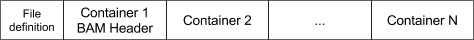
\includegraphics[width=356pt, height=31pt, keepaspectratio=true]{img/CRAMFileFormat2-1-fig001.png}
%%\caption{This should be the caption for \texttt{img/CRAMFileFormat2-1-fig001.png}.}
%%\end{figure}

Pic.1 CRAM file starts with a file definition followed by the BAM header and other 
containers.

Containers consist of one or more blocks. By convention, the BAM header is stored 
in the first container within a single block. This is known as the BAM header block.

%%\begin{figure}[htbp]
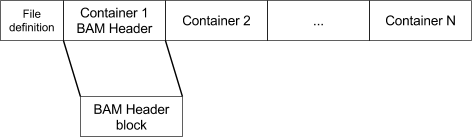
\includegraphics[width=354pt, height=103pt, keepaspectratio=true]{img/CRAMFileFormat2-1-fig002.png}
%%\caption{This should be the caption for \texttt{img/CRAMFileFormat2-1-fig002.png}.}
%%\end{figure}

Pic.2 The BAM header is stored in the first container.

Each container starts with a container header followed by one or more blocks. Each 
block starts with a block header. All data in CRAM is stored within blocks after 
the block header.

%%\begin{figure}[htbp]
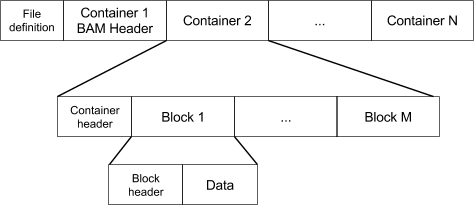
\includegraphics[width=356pt, height=154pt, keepaspectratio=true]{img/CRAMFileFormat2-1-fig003.png}
%%\caption{This should be the caption for \texttt{img/CRAMFileFormat2-1-fig003.png}.}
%%\end{figure}

Pic.3 Container and block structure. All data in CRAM files is stored in blocks.

The first block in each container is the compression header block:

%%\begin{figure}[htbp]
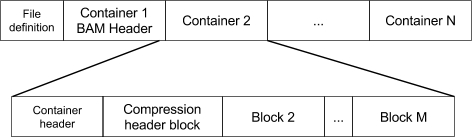
\includegraphics[width=354pt, height=103pt, keepaspectratio=true]{img/CRAMFileFormat2-1-fig004.png}
%%\caption{This should be the caption for \texttt{img/CRAMFileFormat2-1-fig004.png}.}
%%\end{figure}

Pic.4 Compression header is the first block in the container.

The blocks after the compression header are organised logically into slices. One 
slice may contain, for example, a contiguous region of alignment data. Slices begin 
with a slice header block and are followed by one or more data blocks:

%%\begin{figure}[htbp]
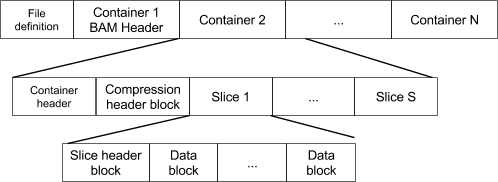
\includegraphics[width=374pt, height=137pt, keepaspectratio=true]{img/CRAMFileFormat2-1-fig005.png}
%%\caption{This should be the caption for \texttt{img/CRAMFileFormat2-1-fig005.png}.}
%%\end{figure}

Pic.5 Containers are logically organised into slices.

Data blocks are divided into core and external data blocks. Each slice must have 
at least one core data block immediately after the slice header block. The core 
data block may be followed by one or more external data blocks.

%%\begin{figure}[htbp]
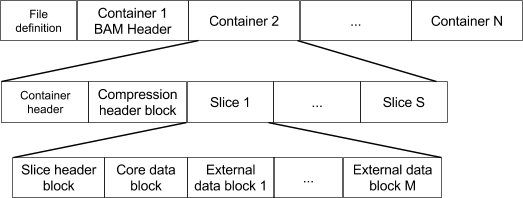
\includegraphics[width=392pt, height=149pt, keepaspectratio=true]{img/CRAMFileFormat2-1-fig006.png}
%%\caption{This should be the caption for \texttt{img/CRAMFileFormat2-1-fig006.png}.}
%%\end{figure}

Pic.5 Data blocks are divided into core and external data blocks. 

\section{\textbf{File definition}}

Each CRAM file starts with a fixed length (26 bytes) definition with the following 
fields:

\begin{tabular}{|l|l|l|}
\hline
\textbf{Data type} & \textbf{Name} & \textbf{Value}\tabularnewline
\hline
byte[4] & format magic number & CRAM (0x43 0x52 0x41 0x4d)\tabularnewline
\hline
unsigned byte & major format number & 3 (0x3)\tabularnewline
\hline
unsigned byte & minor format number & 0 (0x0)\tabularnewline
\hline
byte[20] & file id & CRAM file identifier (e.g. file name or SHA1 checksum)\tabularnewline
\hline
\end{tabular}

Valid CRAM \textit{major}.\textit{minor} version numbers are as follows:

\begin{itemize}
\item[\textit{1.0}]
The original public CRAM release.

\item[\textit{2.0}]
The first CRAM release implemented in both Java and C; tidied up
implementation vs specification differences in \textit{1.0}.

\item[\textit{2.1}]
Gained end of file markers; compatible with \textit{2.0}.

\item[\textit{3.0}]
Additional compression methods; header and data checksums;
improvements for unsorted data.
\end {itemize}

\section{\textbf{Container structure}}

The file definition is followed by one or more containers with the following header 
structure where the container content is stored in the `blocks' field:

\begin{tabular}{|l|>{\raggedright}p{120pt}|>{\raggedright}p{260pt}|}
\hline
\textbf{Data type} & \textbf{Name} & \textbf{Value}
\tabularnewline
\hline
int32 & length & byte size of the container data (blocks)\tabularnewline
\hline
itf8 & reference sequence id & reference sequence identifier  or\linebreak{}
-1 for unmapped reads\linebreak{}
-2 for multiple reference sequences\tabularnewline
\hline
itf8 & starting position on the reference & the alignment start position or\linebreak{}
0 for unmapped reads\tabularnewline
\hline
itf8 & alignment span & the length of the alignment or\linebreak{}
0 for unmapped reads\tabularnewline
\hline
itf8 & number of records & number of records in the container\tabularnewline
\hline
ltf8 & record counter & 1-based sequential index of records in the file/stream.\tabularnewline
\hline
ltf8 & bases & number of read bases\tabularnewline
\hline
itf8 & number of blocks & the number of blocks\tabularnewline
\hline
itf8[ ] & landmarks & Each integer value of this array is a byte offset into the 
blocks byte array. Landmarks are used for random access indexing.\tabularnewline
\hline
int & crc32 & CRC32 hash of the all the preceding bytes in the container.\tabularnewline
\hline
byte[ ] & blocks & The blocks contained within the container.\tabularnewline
\hline
\end{tabular}

\subsection{\textbf{CRAM header in the first container}}

The first container in the CRAM file contains the BAM header in an optionally
compressed block. Only gzip is allowed as compression method for this block. BAM
header is terminated with \textbackslash{}0 byte and any extra bytes in the
block can be used to expand the BAM header. For example when updating @SQ
records additional space may be required for the BAM header. It is recommended
to reserve 50\% more space in the CRAM header block than it is required by the
BAM header.

\section{\textbf{Block structure}}

Containers consist of one or more blocks. Block compression is applied independently 
and in addition to any encodings used to compress data within the block. The block 
have the following header structure with the data stored in the `block data' field:

\begin{tabular}{|l|>{\raggedright}p{120pt}|>{\raggedright}p{260pt}|}
\hline
\textbf{Data type} & \textbf{Name} & \textbf{Value}
\tabularnewline
\hline
byte & method & the block compression method: \linebreak{}
0: raw (none)*\linebreak{}
1: gzip\linebreak{}
2: bzip2\linebreak{}
3: lzma\linebreak{}
4: rans\tabularnewline
\hline
byte & block content type id & the block content type identifier\tabularnewline
\hline
itf8 & block content id & the block content identifier used to associate external 
data blocks with data series\tabularnewline
\hline
itf8 & size in bytes* & size of the block data after applying block compression\tabularnewline
\hline
itf8 & raw size in bytes* & size of the block data before applying block compression\tabularnewline
\hline
byte[ ] & block data & the data stored in the block:\linebreak{}
$\bullet$ bit stream of CRAM records (core data block)\linebreak{}
$\bullet$ byte stream (external data block)\linebreak{}
$\bullet$ additional fields ( header blocks)\tabularnewline
\hline
byte[4] & CRC32 & CRC32 hash value for all preceding bytes in the block\tabularnewline
\hline
\end{tabular}

* Note on raw method: both compressed and raw sizes must be set to the same value.

\subsection{\textbf{Block content types}}

CRAM has the following block content types:

\begin{tabular}{|>{\raggedright}p{143pt}|>{\raggedright}p{45pt}|>{\raggedright}p{116pt}|>{\raggedright}p{114pt}|}
\hline
\textbf{Block content type} & \textbf{Block content type id} & \textbf{Name} & \textbf{Contents}\tabularnewline
\hline
FILE\_HEADER & 0 & BAM header block & BAM header\tabularnewline
\hline
COMPRESSION\_HEADER & 1 & Compression header block & See specific section\tabularnewline
\hline
MAPPED\_SLICE\_HEADER & 2 & Slice header block & See specific section\tabularnewline
\hline
 & 3 &  & reserved\tabularnewline
\hline
EXTERNAL\_DATA & 4 & external data block & data produced by external encodings\tabularnewline
\hline
CORE\_DATA & 5 & core data block & bit stream of all encodings except for external\tabularnewline
\hline
\end{tabular}


\subsection{\textbf{Block content id}}

Block content id is used to distinguish between external blocks in the same slice. 
Each external encoding has an id parameter which must be one of the external block 
content ids. For external blocks the content id is a positive integer. For all 
other blocks content id should be 0. Consequently, all external encodings must 
not use content id less than 1. 

\subsubsection*{Data blocks}

Data is stored in data blocks. There are two types of data blocks: core data blocks 
and external data blocks.The difference between core and external data blocks is 
that core data blocks consist of data series that are compressed using bit encodings 
while the external data blocks are byte compressed. One core data block and any 
number of external data blocks are associated with each slice.

Writing to and reading from core and external data blocks is organised through 
CRAM records. Each data series is associated with an encoding. In case of external 
encoding the block content id is used to identify the block where the data series 
is stored. Please note that external blocks can have multiple data series associated 
with them; in this case the values from these data series will be interleaved. 


\subsection{\textbf{BAM header block}}

The BAM header is stored in a single block within the first container. 

The following constraints apply to the BAM header: 

\begin{itemize}
\item The SQ:MD5 checksum is required unless the reference sequence has been embedded 
into the file.

\item At least one RG record is required.

\item The HD:SO sort order is always POS.
\end{itemize}

\subsection{\textbf{Compression header block}}

The compression header block consists of 3 parts: preservation map, data series 
encoding map and tag encoding map.

\subsubsection*{Preservation map}

The preservation map contains information about which data was preserved in the 
CRAM file. It is stored as a map with byte[2] keys:

\begin{tabular}{|l|l|>{\raggedright}p{100pt}|>{\raggedright}p{220pt}|}
\hline
\textbf{Key} & \textbf{Value data type} & \textbf{Name} & \textbf{Value}\tabularnewline
\hline
RN & bool & read names included & true if read names are preserved for all reads\tabularnewline
\hline
AP & bool & AP data series delta & true if AP data series is delta, false otherwise\tabularnewline
\hline
RR & bool & reference required & true if reference sequence is required to restore 
the data completely\tabularnewline
\hline
SM & byte[5] & substitution matrix & substitution matrix\tabularnewline
\hline
TD & byte[ ] & tag ids dictionary & a list of lists of tag ids, see tag encoding 
section\tabularnewline
\hline
\end{tabular}

\subsubsection*{Data series encodings}

Each data series has an encoding. These encoding are stored in a map with byte[2] 
keys:

\begin{tabular}{|l|l|>{\raggedright}p{100pt}|>{\raggedright}p{220pt}|}
\hline
\textbf{Key} & \textbf{Value data type} & \textbf{Name} & \textbf{Value}\tabularnewline
\hline
BF & encoding\texttt{<}int\texttt{>} & bit flags & see separate section\tabularnewline
\hline
AP & encoding\texttt{<}int\texttt{>} & in-seq positions & 0-based alignment start 
delta from previous record *\tabularnewline
\hline
FP & encoding\texttt{<}int\texttt{>} & in-read positions & positions of the read 
features\tabularnewline
\hline
RL & encoding\texttt{<}int\texttt{>} & read lengths & read lengths\tabularnewline
\hline
DL & encoding\texttt{<}int\texttt{>} & deletion lengths & base-pair deletion lengths\tabularnewline
\hline
NF & encoding\texttt{<}int\texttt{>} & distance to next fragment & number of records 
to the next fragment*\tabularnewline
\hline
BA & encoding\texttt{<}byte\texttt{>} & bases & bases\tabularnewline
\hline
QS & encoding\texttt{<}byte\texttt{>} & quality scores & quality scores\tabularnewline
\hline
BB & encoding\texttt{<}byte[ ]\texttt{>} & stretches of bases & bases\tabularnewline
\hline
QQ & encoding\texttt{<}byte[ ]\texttt{>} & stretches of quality scores & quality scores\tabularnewline
\hline
FC & encoding\texttt{<}byte\texttt{>} & read features codes & see separate section\tabularnewline
\hline
FN & encoding\texttt{<}int\texttt{>} & number of read features & number of read 
features in each record\tabularnewline
\hline
BS & encoding\texttt{<}byte\texttt{>} & base substitution codes & base substitution 
codes\tabularnewline
\hline
IN & encoding\texttt{<}byte[ ]\texttt{>} & insertion & inserted bases\tabularnewline
\hline
RG & encoding\texttt{<}int\texttt{>} & read groups & read groups. Special value 
`-1' stands for no group.\tabularnewline
\hline
MQ & encoding\texttt{<}int\texttt{>} & mapping qualities & mapping quality scores 
 \tabularnewline
\hline
TL & encoding\texttt{<}int\texttt{>} & tag ids  & list of tag ids, see tag encoding 
section\tabularnewline
\hline
RN & encoding\texttt{<}byte[ ]\texttt{>} & read names & read names\tabularnewline
\hline
NS & encoding\texttt{<}int\texttt{>} & next fragment reference sequence id & reference 
sequence ids for the next fragment \tabularnewline
\hline
NP & encoding\texttt{<}int\texttt{>} & next mate alignment start & alignment positions 
for the next fragment\tabularnewline
\hline
TS & encoding\texttt{<}int\texttt{>} & template size & template sizes\tabularnewline
\hline
MF & encoding\texttt{<}int\texttt{>} & next mate bit flags & see specific section\tabularnewline
\hline
CF & encoding\texttt{<}int\texttt{>} & compression bit flags & see specific section\tabularnewline
\hline
TM & encoding\texttt{<}int\texttt{>} & test mark & a prefix expected before every 
record, for debugging purposes.\tabularnewline
\hline
RI & encoding\texttt{<}int\texttt{>} & reference id & record reference id from 
the BAM file header\tabularnewline
\hline
RS & encoding\texttt{<}int\texttt{>} & reference skip length & number of skipped 
bases for the `N' read feature\tabularnewline
\hline
PD & encoding\texttt{<}int\texttt{>} & padding & number of padded bases\tabularnewline
\hline
HC & encoding\texttt{<}int\texttt{>} & hard clip & number of hard clipped bases\tabularnewline
\hline
SC & encoding\texttt{<}byte[ ]\texttt{>} & soft clip & soft clipped bases\tabularnewline
\hline
\end{tabular}

* The data series is reset for each slice. 

\subsubsection*{Encoding tags}

The TL (tag list) data series represents combined information about the number 
of tags in a record and their ids. 

Let $L_{i}=\{T_{i0}, T_{i1}, \ldots, T_{ix}\}$
be sorted list of all tag ids for a record $R_{i}$, where $i$ is the sequential 
record index and $T_{ij}$ denotes $j$-th tag id in the record. We recommend 
alphabetical sort order. The list of unique $L_{i}$ is assigned sequential 
integer numbers starting with 0. These integer numbers represent the TL data series. 
The sorted list of unique $L_{i}$ is stored as the TD value in the preservation 
map. Using TD, an integer from the TL data series can be mapped back into a list 
of tag ids. 

The TD is written as byte array consisting of $L_{i}$ values separated 
with \textbackslash{}0. Each $L_{i}$ value is written as a sequence 
of 3 bytes: tag id followed by tag value type. For example AMiOQZ\textbackslash{}0OQZ\textbackslash{}0, 
where the TD consists of just two values: integer 0 for tags \{AM:i,OQ:Z\} and 
1 for tag \{OQ:Z\}.

\subsubsection*{Encoding tag values}

The encodings used for different tags are stored in a map. The map has integer 
keys composed of the two letter tag abbreviation followed by the tag type as defined 
in the SAM specification, for example `OQZ' for `OQ:Z'. The three bytes form a 
big endian integer and are written as ITF8. For example, 3-byte representation 
of OQ:Z is \{0x4F, 0x51, 0x5A\} and these bytes are intepreted as the integer 0x004F515A. 
The integer is finally written as ITF8.

\begin{tabular}{|l|l|l|>{\raggedright}p{160pt}|}
\hline
\textbf{Key} & \textbf{Value data type} & \textbf{Name} & \textbf{Value}
\tabularnewline
\hline
TAG NAME 1:TAG TYPE 1 & encoding\texttt{<}byte[ ]\texttt{>} & read tag 1 & tag values 
(names and types are available in the data series code)\tabularnewline
\hline
... &  & ... & ...\tabularnewline
\hline
TAG NAME N:TAG TYPE N & encoding\texttt{<}byte[ ]\texttt{>} & read tag N & ...\tabularnewline
\hline
\end{tabular}

Note that tag values are encoded as array of bytes. The routines to convert tag 
values into byte array and back are the same as in BAM with the exception of value 
type being captured in the tag key rather in the value. 

\subsection{\textbf{Slice header block}}

The slice header block is never compressed (block method=raw). For reference mapped 
reads the slice header also defines the reference sequence context of the data 
blocks associated with the slice. Mapped and unmapped reads can be stored within 
the same slice similarly to BAM file. Slices with unsorted reads must not contain 
any other types of reads.

The slice header block contains the following fields.

\begin{tabular}{|l|l|>{\raggedright}p{200pt}|}
\hline
\textbf{Data type} & \textbf{Name} & \textbf{Value}\tabularnewline
\hline
itf8 & reference sequence id & reference sequence identifier or -1 for unmapped 
or unsorted reads\tabularnewline
\hline
itf8 & alignment start & the alignment start position or -1 for unmapped or unsorted 
reads\tabularnewline
\hline
itf8 & alignment span & the length of the alignment or 0 for unmapped or unsorted 
reads\tabularnewline
\hline
itf8 & number of records & the number of records in the slice\tabularnewline
\hline
ltf8 & record counter & 1-based sequential index of records in the file/stream\tabularnewline
\hline
itf8 & number of blocks & the number of blocks in the slice\tabularnewline
\hline
itf8[ ] & block content ids & block content ids of the blocks in the slice\tabularnewline
\hline
itf8 & embedded reference bases block content id & block content id for the embedded 
reference sequence bases or -1 for none\tabularnewline
\hline
byte[16] & reference md5 & MD5 checksum of the reference bases within the slice 
boundaries or 16 \textbackslash{}0 bytes for unmapped or unsorted reads\tabularnewline
\hline
byte[] & optional tags & a series of tag,type,value tuples encoded as
per BAM auxiliary fields.\tabularnewline
\hline
\end{tabular}

The optional tags are encoded in the same manner as BAM tags.  I.e. a
series of binary encoded tags contatenated together where each tag
consists of a 2 byte key (matching [A-Za-z][A-Za-z0-9]) followed by a
1 byte type ([AfZHcCsSiIB]) followed by a string of bytes in a format
defined by the type.

Tags starting in a capital letter are reserved while lowercase ones or
those starting with X, Y or Z are user definable.  Any tag not
understood by a decoder should be skipped over without producing an
error.

At present no tags are defined.

% Details omitted until we fully work through all the corner cases,
% such as seq/qual of *.
%
% Reserved tags are defined as follows:
% 
% \begin{tabular}{|l|l|>{\raggedright}p{325pt}|}
% \hline
% \textbf{Tag type} & \textbf{BAM format} & \textbf{Meaning}\tabularnewline
% \hline
% BD & i & Sum over all reads of the CRC32 hash of sequence base.  This
% may be used to validate round-trips in and out of CRAM.
% calls\tabularnewline
% \hline
% SD & i & Sum over all reads of the CRC32 hash of quality scores. (If
% the quality string is ``*'' in SAM then the hash is of the BAM encoded
% version - a string of bytes with value 255.)\tabularnewline
% \hline
% \end{tabular}


\subsection{\textbf{Core data block}}

A core data block is a bit stream (most significant bit first) consisting of one 
or more CRAM records. Please note that one byte could hold more then one CRAM record 
as a minimal CRAM record could be just a few bits long. The core data block has 
the following fields:

\begin{tabular}{|l|>{\raggedright}p{120pt}|>{\raggedright}p{260pt}|}
\hline
\textbf{Data type} & \textbf{Name} & \textbf{Value}
\tabularnewline
\hline
bit[ ] & CRAM record 1 & The first CRAM record\tabularnewline
\hline
... & ... & ...\tabularnewline
\hline
bit[ ] & CRAM record N & The Nth CRAM record \tabularnewline
\hline
\end{tabular}

\subsection{\textbf{External data block}}

Relationship between core data block and external data blocks is shown in the following 
picture: 

%%\begin{figure}[htbp]
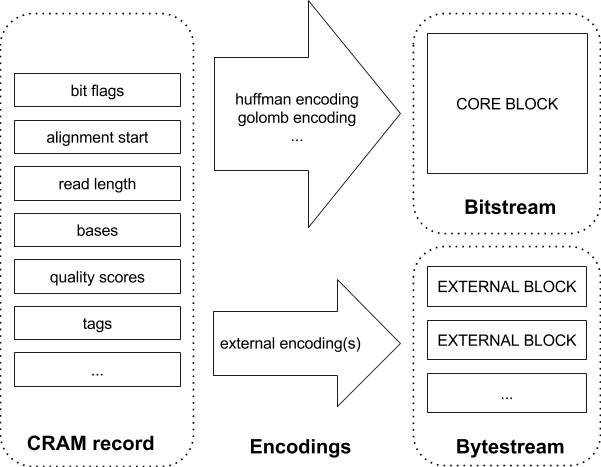
\includegraphics[width=451pt, height=350pt, keepaspectratio=true]{img/CRAMFileFormat2-1-fig007.png}
%%\caption{This should be the caption for \texttt{img/CRAMFileFormat2-1-fig007.png}.}
%%\end{figure}

Pic.3 Relationship between core data block and external data blocks.

The picture shows how a CRAM record (on the left) is partially written to core 
data block while the other fields are stored in two external data blocks. The specific 
encodings are presented only for demonstration purposes, the main point here is 
to distinguish between bit encodings whose output is always stored in core data 
block and the external encoding which simply stored the bytes into external data 
blocks.

\section{\textbf{End of file marker}}

A special container is used to mark the end of a file or stream. It is required in version 3 or later. The idea is to provide an easy and a quick way to detect that a CRAM file or stream is complete. The marker is basically an empty container with ref seq id set to -1 (unaligned) and alignment 
start set to 4542278.

Here is a complete content of the EOF container explained in detail:

\begin{tabular}{|l|l|>{\raggedright}p{150pt}|>{\raggedright}p{180pt}|}
\hline
\textbf{hex bytes} & \textbf{data type} & \textbf{decimal value} & \textbf{field 
name}\tabularnewline
\hline
\multicolumn{4}{|l|}{\textit{Container header}}\tabularnewline
\hline
0f 00 00 00 & integer & 15 & size of blocks data\tabularnewline
\hline
ff ff ff ff 0f & itf8 & -1 & ref seq id\tabularnewline
\hline
e0 45 4f 46 & itf8 & 4542278 & alignment start\tabularnewline
\hline
00 & itf8 & 0 & alignment span\tabularnewline
\hline
00 & itf8 & 0 & nof records\tabularnewline
\hline
00 & itf8 & 0 & global record counter\tabularnewline
\hline
00 & itf8 & 0 & bases\tabularnewline
\hline
01 & itf8 & 1 & block count\tabularnewline
\hline
00 & array & 0 & landmarks\tabularnewline
\hline
05 bd d9 4f & integer & 1339669765 & container header CRC32\tabularnewline
\hline
\multicolumn{4}{|l|}{\textit{Compression header block}}\tabularnewline
\hline
00 & byte & 0 (RAW) & compression method\tabularnewline
\hline
01 & byte & 1 (COMPRESSION\_HEADER) & block content type\tabularnewline
\hline
00 & itf8 & 0 & block content id\tabularnewline
\hline
06 & itf8 & 6 & compressed size\tabularnewline
\hline
06 & itf8 & 6 & uncompressed size\tabularnewline
\hline
\multicolumn{4}{|l|}{\textit{Compression header}}\tabularnewline
\hline
01 & itf8 & 1 & preservation map byte size\tabularnewline
\hline
00 & itf8 & 0 & preservation map size\tabularnewline
\hline
01 & itf8 & 1 & encoding map byte size\tabularnewline
\hline
00 & itf8 & 0 & encoding map size\tabularnewline
\hline
01 & itf8 & 1 & tag encoding byte size\tabularnewline
\hline
00 & itf8 & 0 & tag encoding map size\tabularnewline
\hline
ee 63 01 4b & integer & 1258382318 & block CRC32\tabularnewline
\hline
\end{tabular}

When compiled together the EOF marker is 38 bytes long and in hex representation 
is:

0f 00 00 00 ff ff ff ff 0f e0 45 4f 46 00 00 00 00 01 00 05 bd d9 4f 00 01 00 06 06 01 00 01 00 01 00 ee 63 01 4b

\section{\textbf{Record structure}}

CRAM record is based on the SAM record but has additional features allowing for 
more efficient data storage.  In contrast to BAM record CRAM record uses bits as 
well as bytes for data storage. This way, for example, various coding techniques 
which output variable length binary codes can be used directly in CRAM. On the 
other hand, data series that do not require binary coding can be stored separately 
in external blocks with some other compression applied to them independently.

\subsection{\textbf{CRAM record}}

Both mapped and unmapped reads start with the following fields. Please note that 
the data series type refers to the logical data type and the data series name corresponds 
to the data series encoding map.

\begin{tabular}{|>{\raggedright}p{36pt}|>{\raggedright}p{70pt}|>{\raggedright}p{75pt}|>{\raggedright}p{90pt}|>{\raggedright}p{171pt}|}
\hline
 & \textbf{Data series type} & \textbf{Data series name} & \textbf{Field} & \textbf{Description}\tabularnewline
\hline
1 & int & BF & CRAM bit flags & see CRAM record bit flags\tabularnewline
\hline
2 & int & CF  & compression bit flags & see compression bit flags\tabularnewline
\hline
3 & int & RI & ref id & reference sequence id, not used for single reference slices, 
reserved for future multiref slices. \tabularnewline
\hline
4 & int & RL & read length & the length of the read\tabularnewline
\hline
5 & int & AP & alignment start & the alignment start position *1\tabularnewline
\hline
6 & int & RG & read group & the read group identifier\tabularnewline
\hline
7 & byte & QS & quality scores & quality scores are stored depending on the value 
of the `mapped QS included' field\tabularnewline
\hline
8 & byte[ ] & RN & read name & the read names (if preserved)\tabularnewline
\hline
9 & *2 & *2 & mate record & *2 (if not the last record)\tabularnewline
\hline
10 & int & TL & tag ids & tag ids *3\tabularnewline
\hline
11 & byte[ ] & - & tag values & tag values *3\tabularnewline
\hline
\end{tabular}

*1 The AP data series is delta encoded for reads mapped to a single reference slice 
and normal integer value in all other cases. 

*2 See \emph{mate record} section.

*3 See\emph{ tag encoding} section.

The CRAM record structure for mapped reads has the following additional fields:

\begin{tabular}{|>{\raggedright}p{36pt}|>{\raggedright}p{70pt}|>{\raggedright}p{74pt}|>{\raggedright}p{85pt}|>{\raggedright}p{177pt}|}
\hline
 & \textbf{Data series type} & \textbf{Data series name} & \textbf{Field} & \textbf{Description}\tabularnewline
\hline
1 & *1 & *1 & read feature records & *1\tabularnewline
\hline
2 & byte & MQ & mapping quality & read mapping quality\tabularnewline
\hline
\end{tabular}

*1 See read feature record specification below.

The CRAM record structure for unmapped reads has the following additional fields:

\begin{tabular}{|>{\raggedright}p{8pt}|>{\raggedright}p{88pt}|>{\raggedright}p{83pt}|>{\raggedright}p{85pt}|>{\raggedright}p{178pt}|}
\hline
 & \textbf{Data series type} & \textbf{Data series name} & \textbf{Field} & \textbf{Description}\tabularnewline
\hline
1 & byte[read length] & BA & bases & the read bases\tabularnewline
\hline
\end{tabular}

\subsection{\textbf{Read bases}}

CRAM format supports ACGTN bases only. All non-ACGTN read bases must be replaced 
with N (unknown) base. In case of mismatching non-ACGTN read base and non-ACGTN 
reference base a ReadBase read feature should be used to capture the fact that 
the read base should be restored as N base. 

\subsection{\textbf{CRAM record bit flags (BF data series)}}

The following flags are defined for each CRAM read record:

\begin{tabular}{|>{\raggedright}p{144pt}|>{\raggedright}p{144pt}|>{\raggedright}p{144pt}|}
\hline
\textbf{Bit flag} & \textbf{Comment} & \textbf{Description}\tabularnewline
\hline
0x1 & ! 0x40 \&\& ! 0x80 & template having multiple segments in sequencing\tabularnewline
\hline
0x2 &  & each segment properly aligned according to the aligner\tabularnewline
\hline
0x4 &  & segment unmapped\tabularnewline
\hline
0x8 & calculated* or stored in the mate's info & next segment in the template unmapped\tabularnewline
\hline
0x10 &  & SEQ being reverse complemented\tabularnewline
\hline
0x20 & calculated* or stored in the mate's info & SEQ of the next segment in the 
template being reversed\tabularnewline
\hline
0x40 &  & the first segment in the template\tabularnewline
\hline
0x80 &  & the last segment in the template\tabularnewline
\hline
0x100 &  & secondary alignment\tabularnewline
\hline
0x200 &  & not passing quality controls\tabularnewline
\hline
0x400 &  & PCR or optical duplicate\tabularnewline
\hline
\end{tabular}

* For segments within the same slice.

\subsection{\textbf{Read feature records}}

Read features are used to store read details that are expressed using read coordinates 
(e.g. base differences respective to the reference sequence). The read feature 
records start with the number of read features followed by the read features themselves:

\begin{tabular}{|>{\raggedright}p{36pt}|>{\raggedright}p{65pt}|>{\raggedright}p{84pt}|>{\raggedright}p{90pt}|>{\raggedright}p{168pt}|}
\hline
 & \textbf{Data series type} & \textbf{Data series name} & \textbf{Field} & \textbf{Description}\tabularnewline
\hline
1 & int & FN & number of read features & the number of read features\tabularnewline 
\hline
2\textsuperscript{*1}  & int & FP & in-read-position & position of the read feature\tabularnewline 
\hline
3\textsuperscript{*1} & byte & FC & read feature code & \textsuperscript{*2}\tabularnewline
\hline
4\textsuperscript{*1} & \textsuperscript{*2} & \textsuperscript{*2} & read feature data & \textsuperscript{*2}\tabularnewline
\hline
\end{tabular}

*1 Repeated for each read feature.

*2 See \emph{read feature codes} below.

\subsubsection*{Read feature codes}

The following codes are used to distinguish variations in read coordinates:

\begin{tabular}{|>{\raggedright}p{91pt}|>{\raggedright}p{45pt}|>{\raggedright}p{72pt}|>{\raggedright}p{66pt}|>{\raggedright}p{132pt}|}
\hline
\textbf{Feature code} & \textbf{Id} & \textbf{Data series type} & \textbf{Data 
series name} & \textbf{Description}\tabularnewline
\hline
Bases & b (0x62) & byte[ ] & BB & a stretch of bases\tabularnewline
\hline
Scores & q (0x71) & byte[ ] & QQ & a stretch of scores\tabularnewline
\hline
% Neither C nor Java implementations generator nor can decode the 'A'
% feature code, but if they did they'd be BB/QQ and not BA/QS.  Best
% to omit it from published spec for now?
%
% Bases and scores & A (0x41) & byte[ ],byte[ ] & BB,QQ & A a stretch of bases and
% quality scores score\tabularnewline
% \hline
Read base & B (0x42) & byte,byte & BA,QS & A base and associated quality score\tabularnewline
\hline
Substitution & X (0x58) & byte & BS & base substitution codes, SAM operators X, 
M and =\tabularnewline
\hline
Insertion & I (0x49) & byte[ ] & IN & inserted bases, SAM operator I\tabularnewline
\hline
Deletion & D (0x44) & int & DL & number of deleted bases, SAM operator D\tabularnewline
\hline
Insert base & i (0x69) & byte & BA & single inserted base, SAM operator I\tabularnewline
\hline
Quality score & Q (0x51) & byte & QS & single quality score\tabularnewline
\hline
Reference skip & N (0x4E) & int & RS & number of skipped bases, SAM operator N\tabularnewline
\hline
Soft clip & S (0x53) & byte[ ] & SC & soft clipped bases, SAM operator S\tabularnewline
\hline
Padding & P (0x50) & int & PD & number of padded bases, SAM operator P\tabularnewline
\hline
Hard clip & H (0x48) & int & HC & number of hard clipped bases, SAM operator H\tabularnewline
\hline
\end{tabular}

\subsubsection*{Base substitution codes (BS data series)}

A base substitution is defined as a change from one nucleotide base (reference 
base) to another (read base) including N as an unknown or missing base. There are 
5 possible bases ACGTN, 4 possible substitutions for each base and 20 substitutions 
in total. Substitutions for the same reference base are assigned integer codes 
from 0 to 3 inclusive. To restore a base one would need to know its substitution 
code and the reference base. 

A base substitution matrix assigns integer codes to all possible substitutions. 

Substitution matrix is written as follows. Substitutions for a given reference 
base are sorted by their frequencies in descending order then assigned numbers 
from 0 to 3. Same-frequency ties are broken using alphabetical order. For example, 
let us assume the following substitution frequencies for base A: 

AC: 15\%

AG: 25\%

AT: 55\%

AN: 5\%

Then the substitution codes are: 

AC: 2

AG: 1

AT: 0

AN: 3

and they are written as a single byte, 10 01 00 11 = 147 decimal or 0x93 in this 
case. The whole substitution matrix is written as 5 bytes, one for each reference 
base in the alphabetical order: A, C, G, T and N.

Note: the last two bits of each substitution code are redundant but still required 
to simplify the reading. 

\subsection{\textbf{Mate record}}

There are two ways in which mate information can be preserved in CRAM: number of 
records downstream (distance) to the next fragment in the template and a special 
mate record if the next fragment is not in the current slice. Combination of the 
two approaches allows to fully restore BAM level mate information and efficiently 
store it in the CRAM file. 

For mates within the slice only the distance is captured:

\begin{tabular}{|>{\raggedright}p{7pt}|>{\raggedright}p{68pt}|>{\raggedright}p{115pt}|>{\raggedright}p{228pt}|}
\hline
 & \textbf{Data series type} & \textbf{Data series name} & \textbf{Description}\tabularnewline
\hline
1 & int & NF & the number of records to the next fragment\tabularnewline
\hline
\end{tabular}

If the next fragment is not found within the horizon then the following structure 
is included into the CRAM record:

\begin{tabular}{|>{\raggedright}p{6pt}|>{\raggedright}p{66pt}|>{\raggedright}p{117pt}|>{\raggedright}p{228pt}|}
\hline
 & \textbf{Data series type} & \textbf{Data series name} & \textbf{Description}\tabularnewline
\hline
1 & byte & MF & next mate bit flags, see table below\tabularnewline
\hline
2 & byte[ ] & RN & the read name\tabularnewline
\hline
3 & int & NS & mate reference sequence identifier \tabularnewline
\hline
4 & long & NP & mate alignment start position \tabularnewline
\hline
5 & int & TS & the size of the template (insert size)\tabularnewline
\hline
\end{tabular}

\subsubsection*{}

\subsubsection*{Next mate bit flags (MF data series)}

The next mate bit flags expressed as an integer represent the MF data series. The 
following bit flags are defined:

\begin{tabular}{|>{\raggedright}p{47pt}|>{\raggedright}p{134pt}|>{\raggedright}p{250pt}|}
\hline
\textbf{Bit flag} & \textbf{Name} & \textbf{Description}\tabularnewline
\hline
0x1 & mate negative strand bit & the bit is set if the mate is on the negative 
strand\tabularnewline
\hline
0x2 & mate mapped bit & the bit is set if the mate is mapped\tabularnewline
\hline
\end{tabular}

\subsubsection*{Read names (RN data series)}

Read names can be preserved in the CRAM format. However, it is anticipated that 
in the majority of cases original read names will not be preserved and sequential 
integer numbers will be used as read names. Read names may also be used to associate 
fragments into templates when the fragments are too far apart to be referenced 
by the number of CRAM records. In this case the read names are not required to 
be the same as the original ones. Their only two requirements are:

$\bullet$ read name must be the same for all fragments of the same template

$\bullet$ read name of a template must be unique within a file

\subsection{\textbf{Compression bit flags (CF data series)}}

The compression bit flags expressed as an integer represent the CF data series. 
The following compression flags are defined for each CRAM read record:

\begin{tabular}{|>{\raggedright}p{39pt}|>{\raggedright}p{150pt}|>{\raggedright}p{242pt}|}
\hline
\textbf{Bit flag} & \textbf{Name} & \textbf{Description}\tabularnewline
\hline
0x1 & quality scores stored as array & quality scores can be stored as read features 
or as an array similar to read bases.\tabularnewline
\hline
0x2 & detached & the next segment is out of horizon\tabularnewline
\hline
0x4 & has mate downstream & tells if the next segment should be expected further 
in the stream\tabularnewline
\hline
0x8 & decode sequence as ``*'' & informs the decoder that the sequence
is unknown and that any encoded reference differences are present only to
recreate the CIGAR string.\tabularnewline
\hline
\end{tabular}

\section{\textbf{Reference sequences}}

CRAM format is natively based upon usage of reference sequences even though in 
some cases they are not required. In contrast to BAM format CRAM format has strict 
rules about reference sequences. 

\begin{enumerate}
\item M5 (sequence MD5 checksum) field of @SQ sequence record in the BAM header is 
required and UR (URI for the sequence fasta optionally gzipped file) field is strongly 
advised. The rule for calculating MD5 is to remove any non-base symbols (like \textbackslash{}n, 
sequence name or length and spaces) and upper case the rest. Here are some examples: 

\texttt{> samtools faidx human\_g1k\_v37.fasta 1 \textbar{} grep -v '\textasciicircum{}>' \textbar{} tr -d '\textbackslash{}n' \textbar{} tr a-z A-Z \textbar{} md5sum -\\
1b22b98cdeb4a9304cb5d48026a85128  -}

\texttt{> samtools faidx human\_g1k\_v37.fasta 1:10-20 \textbar{}grep -v '\textasciicircum{}\texttt{>}' \textbar{}tr -d '\textbackslash{}n' \textbar{}tr a-z A-Z \textbar{}md5sum -\\
0f2a4865e3952676ffad2c3671f14057  -}

Please note that the latter calculates the checksum for 11 bases from position 
10 (inclusive) to 20 (inclusive) and the bases are counted 1-based, so the first 
base position is 1. 

\item All CRAM reader implementations are expected to check for reference MD5 checksums 
and report any missing or mismatching entries. Consequently, all writer implementations 
are expected to ensure that all checksums are injected or checked during compression 
time. 

\item In some cases reads may be mapped beyond the reference sequence. All out of 
range reference bases are all assumed to be `N'. 

\item MD5 checksum bytes in slice header should be ignored for unmapped or multiref 
slices. 
\end{enumerate}

\section{\textbf{Indexing}}

\subsubsection*{General notes}

Please note that CRAM indexing is external to the file format itself and may change 
independently of the file format specification in the future. For example, a new 
type of index files may appear. 

Individual records are not indexed in CRAM files, slices should be used instead 
as a unit of random access. Another important difference between CRAM and BAM indexing 
is that CRAM container header and compression header block (first block in container) 
must always be read before decoding a slice. Therefore two read operations are 
required for random access in CRAM.

Indexing a CRAM file is deemed to be a lightweight operation because it does not 
require any CRAM records to be read. All indexing information can be obtained from 
container headers, namely sequence id, alignment start and span, container start 
byte offset and slice byte offset inside the container. 

\subsubsection*{CRAM index}

A CRAM index is a gzipped tab delimited file containing the following columns:

\begin{enumerate}
\item Sequence id

\item Alignment start

\item Alignment span

\item Container start byte offset in the file

\item Slice start byte offset in the container data (`blocks')

\item Slice bytes
\end{enumerate}

Each line represents a slice in the CRAM file. Please note that all slices must 
be listed in index file.

\subsubsection*{BAM index}

BAM indexes are supported by using 4-byte integer pointers called landmarks that 
are stored in container header. BAM index pointer is a 64-bit value with 48 bits 
reserved for the BAM block start position and 16 bits reserved for the in-block 
offset. When used to index CRAM files, the first 48 bits are used to store the 
CRAM container start position and the last 16 bits are used to store the index 
of the landmark in the landmark array stored in  container header. The landmark 
index can be used to access the appropriate slice. 

The above indexing scheme treats CRAM slices as individual records in BAM file. 
This allows to apply BAM indexing to CRAM files, however it introduces some overhead 
in seeking specific alignment start because all preceding records in the slice 
must be read and discarded.

\section{\textbf{Appendix}}

\subsection{\textbf{External encoding}}

External encoding operates on bytes only. Therefore any data series must be translated 
into bytes before sending data into an external block. The following agreements 
are defined. 

Integer values are written as ITF8, which then can be translated into an array 
of bytes. 

Strings, like read name, are translated into bytes according to UTF8 rules. In 
most cases these should coincide with ASCII, making the translation trivial. 

\subsection{\textbf{rANS codec}}

rANS is the range-coder variant of the Asymmetric Numerical
System\footnote{J. Duda, \textit{Asymmetric numeral systems: entropy
    coding combining speed of Huffman coding with compression rate of
    arithmetic coding}, \url{http://arxiv.org/abs/1311.2540}}.

The structure of the external rANS codec consists of several
components: meta-data consisting of compression-order, and compressed
and uncompressed sizes; normalised frequencies of the alphabet systems
to be encoded, either in Order-0 or Order-1 context; and the rANS
encoded byte stream itself.

Here "Order" refers to the number of bytes of context used in
computing the frequencies. It will be 0 or 1.  Ignoring punctuation
and space, an Order-0 analysis of English text may observe that `e' is
the most common letter (12-13\%), and that `u' occurs only around 2.5\%
of the time.  If instead we consider the frequency of a letter in the
context of one previous letter (Order-1) then these statistics change
considerably;  we know that if the previous letter was `q' then `e'
becomes a rare letter while `u' is the most likely.

These observed frequencies are directly related to the amount of
storage required to encode a symbol (e.g. an alphabet
letter)\footnote{ C.E. Shannon, \textit{A Mathematical Theory of
    Communication}, Bell System Technical Journal, vol. 27,
    pp. 379-423, 623-656, July, October, 1948}.


\subsubsection{\textbf{rANS compressed data structure}}
A compressed data block consists of the following logical parts: 


\begin{tabular}{|l|l|>{\raggedright}p{100pt}|>{\raggedright}p{220pt}|}
\hline
\textbf{Value data type} & \textbf{Name} & \textbf{Description}\tabularnewline
\hline
byte & order & the order of the codec, either 0 or 1\tabularnewline
\hline
int & compressed size & the size in bytes of frequency table and compressed blob\tabularnewline
\hline
int & data size & raw or uncompressed data size in bytes\tabularnewline
\hline
byte[] & frequency table & byte frequencies of input data written using RLE\tabularnewline
\hline
byte[] & compressed blob & compressed data\tabularnewline
\hline
\end{tabular}

\subsubsection{\textbf{Frequency table}}

The alphabet used here is simply byte values, so a maximum of 256
symbols as some values may not be present.

The symbol frequency table indicates which symbols are present and
what their relative frequencies are.  The total sum of symbol
frequencies are normalised to add up to 4095.

Formally, this is an ordered alphabet $\mathbb{A}$ containing symbols $s$ where
$s_{i}$ with the $i$-th symbol in $\mathbb{A}$, occuring with the frequency $freq_{i}$.

\textbf{Order-0 encoding}

The normalised symbol frequencies are then written out as \{symbol,
frequency\} pairs in ascending order of symbol (0 to 255 inclusive).
If a symbol has a frequency of 0 then it is omitted.

To avoid storing long consecutive runs of symbols if all are present
(eg a-z in a long piece of English text) we use run-length-encoding on
the alphabet symbols.  If two consecutive symbols have non-zero
frequencies then a counter of how many other non-zero frequency
consecutive symbols is output directly after the second consecutive
symbol, with that many symbols being subsequently omitted. 

For example for non-zero frequency symbols `a', `b', `c', `d' and `e'
we would write out symbol `a', `b' and the value 3 (to indicate `c',
`d' and `e' are also present).

The frequency is output after every symbol (whether explicit or
implicit) using ITF8 encoding. This means that frequencies 0-127 are
encoded in 1 byte while frequencies 128-4095 are encoded in 2 bytes.

Finally the symbol 0 is written out to indicate the end of the
symbol-frequency table.

As an example, take the string \texttt{abracadabra}.

\begin{minipage}[t]{0.5\textwidth}
Symbol frequency:
\\[8pt]
\begin{tabular}{ |r|r| }
\hline
Symbol & Frequency\\
\hline
a & 5 \\
b & 2 \\
c & 1 \\
d & 1 \\
r & 2 \\
\hline
\end{tabular}
\end{minipage}
\begin{minipage}[t]{0.5\textwidth}
Normalised to sum to 4095:
\\[8pt]
\begin{tabular}{ |r|r|}
\hline
Symbol & Frequency\\
\hline
a & 1863 \\
b &  744 \\
c &  372 \\
d &  372 \\
r &  744 \\
\hline
\end{tabular}
\end{minipage}

Encoded as:
\begin{verbatim}
0x61      0x87 0x47      # `a'           <1863>
0x62 0x02 0x82 0xe8      # `b' <+2: c,d>  <744>
          0x81 0x74      # `c' (implicit) <372> 
          0x81 0x74      # `d' (implicit) <372> 
0x72      0x82 0xe8      # `r'            <744> 
0x00                     # <0>          
\end{verbatim}


\textbf{Order-1 encoding}

To encode Order-1 statistics typically requires a larger table as for
an $N$ sized alphabet we need to potentially store an $N$x$N$ matrix.
We store these as a series of Order-0 tables.

We start with the outer context byte, emitting the symbol if it is
non-zero frequency.  We perform the same run-length-encoding as we
use for the Order-0 table and end the contexts with a nul byte.  After
each context byte we emit the Order-0 table relating to that context.

One last caveat is that we have no context for the first byte in the
data stream (infact for 4 equally spaced starting points, see
``interleaving" below).  We use the ASCII value (`\textbackslash0') as
the starting context and so need to consider this in our frequency
table.

Consider \texttt{abracadabraabracadabraabracadabraabracadabra} as
example input.

\begin{minipage}[t]{0.5\textwidth}
Observed Order-1 frequencies:
\\[8pt]
\begin{tabular}{ |r|r|r| }
\hline
Context & Symbol & Frequency\\
\hline
\textbackslash0 & a & 4 \\
\hline
a & a & 3 \\
  & b & 8 \\
  & c & 4 \\
  & d & 4 \\
\hline
b & r & 8 \\
\hline
c & a & 4 \\
\hline
d & a & 4 \\
\hline
r & a & 8 \\
\hline
\end{tabular}
\end{minipage}
\begin{minipage}[t]{0.5\textwidth}
Normalised (per Order-0 statistics):
\\[8pt]
\begin{tabular}{ |r|r|r|}
\hline
Context & Symbol & Frequency\\
\hline
\textbackslash0 & a & 4095 \\
\hline
a & a &  646 \\
  & b & 1725 \\
  & c &  862 \\
  & d &  862 \\
\hline
b & r & 4095 \\
\hline
c & a & 4095 \\
\hline
d & a & 4095 \\
\hline
r & a & 4095 \\
\hline
\end{tabular}
\end{minipage}


Encoded as:
\begin{verbatim}
0x00                 # `\0' context
0x61      0x8f 0xff  # a  <4095>
0x00                 # end of Order-0 table

0x61                 # `a' context
0x61      0x82 0x86  # a            <646>
0x62 0x02 0x86 0xbd  # b <+2: c,d> <1725>
          0x83 0x5e  # c (implicit) <862>
          0x83 0x5e  # d (implicit) <862>
0x00                 # end of Order-0 table

0x62 0x02            # `b' context, <+2: c, d>
0x72      0x8f 0xff  # r <4095>
0x00                 # end of Order-0 table

                     # `c' context (implicit)
0x61      0x8f 0xff  # a <4095>
0x00                 # end of Order-0 table

                     # `d' context (implicit)
0x61      0x8f 0xff  # a <4095>
0x00                 # end of Order-0 table

0x72                 # `r' context
0x61      0x8f 0xff  # a <4095>
0x00                 # end of Order-0 table

0x00                 # end of contexts
\end{verbatim}


\subsubsection{rANS entropy encoding}

The encoder takes a symbol $s$ and a current state $x$ (initially zero) to
produce a new state $x'$ with function $C$.

{
\setlength{\parindent}{1cm}
\indent $x' = C(s,x)$
}

The decoding function $D$ is the inverse of $C$ such that $C(D(x)) = x$.

{
\setlength{\parindent}{1cm}
\indent $D(x') = (s,x)$
}

The entire encoded message can be viewed as a series of nested $C$
operations, with decoding yielding the symbols in reverse order, much
like popping items off a stack.  This is where the asymmetric part of
ANS comes from.

As we encode into $x$ the value will grow, so for efficiency we ensure
that it always fits within known bounds. This is governed by

{
\setlength{\parindent}{1cm}
\indent $L \leq x < bL-1$
}


where $b$ is the base and $L$ is the lower-bound.

We ensure this property is true before every use of $C$ and after every
use of $D$.  Finally to end the stream we flush any remaining data out
by storing the end state of $x$.


\textbf{Implementation specifics}

We use an unsigned 32-bit integer to hold $x$. In encoding it is
initialised to zero. For decoding it is read little-endian from the
input stream.

Recall $freq_{i}$ is the frequency of the $i$-th symbol $s_{i}$ in alphabet
$\mathbb{A}$.  We define $cfreq_i$ to be cumulative frequency of all symbols
up to but not including $s_{i}$:

{
\setlength{\parindent}{1cm}
$ cfreq_{i} = \left\{
\begin{array}{l l}
0 & \quad \textrm{if $i < 1$} \\
cfreq_{i-1} + freq_{i-1} & \quad \textrm{if $i \geq 1$}
\end{array}
\right. $
% \\*[8pt]
% \indent $cfreq_{i} = \displaystyle \sum_{j=0}^{i-1} freq_j$
}


We have a reverse lookup table $cfreq\_to\_sym_c$ from 0 to 4095
(0xfff) that maps a cumulative frequency $c$ to a symbol $s$.

{
\setlength{\parindent}{1cm}
\indent   $cfreq\_to\_sym_c = s_{i} \quad | \quad c: \enskip cfreq_i \leq c <
cfreq_i + freq_i$
% \\*[8pt]
% \indent   $cfreq\_to\_sym_c = s_{i} ,
% \quad \forall c \in [cfreq_i, cfreq_i + freq_i)$
}


The $x' = C(s,x)$ function used for the ${i}-th symbol ${s} is:

{
\setlength{\parindent}{1cm}
\indent    $x' = (x/freq_i) * \mathtt{0x1000} + cfreq_i + (x\%freq_i)$
}

The $D(x') = (s,x)$ function used to produce the $i$-th symbol $s$ and
a new state $x$ is:

{
\setlength{\parindent}{1cm}
\indent    $c = x' \& \mathtt{0xfff}$\\*
\indent    $s_{i} = cfreq\_to\_sym_{c}$\\*
\indent    $x = freq_{i} (x' / \mathtt{0x1000}) + c - cfreq_{i}$
}

Most of these operations can be implemented as bit-shifts and bit-AND,
with the encoder modulus being implemented as a multiplication by the
reciprocal, computed once only per alphabet symbol.

We use $L = \mathtt{0x800000}$ and $b = 256$, permitting us to flush out one byte
at a time (encoded and decoded in reverse order).

Before every encode $C(s,x)$ we renormalise $x$, shifting out the bottom 8
bits of $x$ until $x < \mathtt{0x80000} * freq_i$.  After finishing encoding we
flush 4 more bytes (lowest 8-bits first) from $x$.

After every decoded $D(x')$ we renormalise $x'$, shifting in the bottom 8
bits until $x \geq \mathtt{0x800000}$.


\textbf{Interleaving}

For efficiency, we interleave 4 separate rANS codecs at the same
time\footnote{F. Giesen, \textit{Interleaved entropy coders},
  \url{http://arxiv.org/abs/1402.3392}}.  For the Order-0 codecs these
simply encode or decode the 4 neighbouring bytes in cyclic fashion
using interleaved codec 1, 2, 3 and 4, sharing the same output buffer
(so the output bytes get interleaved).

For the Order-1 codec we cannot do this as we need to know the
previous byte value as the context for the next byte.  Therefore split
the input data into 4 approximately equal sized
fragments\footnote{This was why the `\textbackslash0' $\to$ `a'
  context in the example above had a frequency of 4 instead of 1.}
starting at $0$, $\lfloor{}len/4\rfloor{}*1$,
$\lfloor{}len/4\rfloor{}*2$ and $\lfloor{}len/4\rfloor{}*3$.  Each
Order-1 codec operates in a cyclic fashion as with Order-0, all
starting with 0 as their state and sharing the same output buffer. Any
remainder, when the input buffer is not divisible by 4, is encoded at
the end by the 4th encoder.

We do not permit Order-1 encoding of data streams smaller than 4
bytes.

\subsection{\textbf{Codings}}

\subsubsection*{Introduction}

The basic idea for codings is to efficiently represent some values in binary format. 
This can be achieved in a number of ways that most frequently involve some knowledge 
about the nature of the values being encoded, for example, distribution statistics. 
The methods for choosing the best encoding and determining its parameters are very 
diverse and are not part of the CRAM format specification, which only describes 
how the information needed to decode the values should be stored.

\subsubsection*{Offset}

Most of the codings listed below encode positive integer numbers. An integer offset 
value is used to allow any integer numbers and not just positive ones to be encoded. 
It can also be used for monotonically decreasing distributions with the maximum 
not equal to zero. For example, given offset is 10 and the value to be encoded 
is 1, the actually encoded value would be offset+value=11. Then when decoding, 
the offset would be subtracted from the decoded value. 

\subsubsection*{Beta coding}

\subsubsection*{Definition}

Beta coding is a most common way to represent numbers in \emph{binary notation}. 


\subsubsection*{Examples}

\begin{tabular}{|>{\raggedright}p{222pt}|>{\raggedright}p{222pt}|}
\hline
\textbf{Number} & \textbf{Codeword}\tabularnewline
\hline
0 & 0\tabularnewline
\hline
1 & 1\tabularnewline
\hline
2 & 10\tabularnewline
\hline
4 & 100\tabularnewline
\hline
\end{tabular}

\subsubsection*{Parameters}

CRAM format defines the following parameters of beta coding: 

\begin{tabular}{|>{\raggedright}p{144pt}|>{\raggedright}p{144pt}|>{\raggedright}p{144pt}|}
\hline
\textbf{Data type} & \textbf{Name} & \textbf{Comment}\tabularnewline
\hline
itf8 & offset & offset is added to each value\tabularnewline
\hline
itf8 & length & the number of bits used\tabularnewline
\hline
\end{tabular}

\subsubsection*{Gamma coding}

\subsubsection*{Definition}

\emph{Elias gamma code} is a prefix encoding of positive integers. This is a combination 
of unary coding and beta coding. The first is used to capture the number of bits 
required for beta coding to capture the value. 

\subsubsection*{Encoding}

\begin{enumerate}
\item Write it in binary.

\item Subtract $1$ from the number of bits written in step 1 and prepend that many zeros.

\item An equivalent way to express the same process:

\item Separate the integer into the highest power of $2$ it contains ($2N$) and the remaining 
$N$ binary digits of the integer.

\item Encode $N$ in unary; that is, as $N$ zeroes followed by a one.

\item Append the remaining $N$ binary digits to this representation of $N$.
\end{enumerate}

\subsubsection*{Decoding}

\begin{enumerate}
\item Read and count 0s from the stream until you reach the first 1. Call this count 
of zeroes $N$.

\item Considering the one that was reached to be the first digit of the integer, with 
a value of $2N$, read the remaining $N$ digits of the integer.
\end{enumerate}

\subsubsection*{Examples}

\begin{tabular}{|>{\raggedright}p{76pt}|>{\raggedright}p{107pt}|}
\hline
\textbf{Value} & \textbf{Codeword}\tabularnewline
\hline
1 & 1\tabularnewline
\hline
2 & 010\tabularnewline
\hline
3 & 011\tabularnewline
\hline
4 & 00100\tabularnewline
\hline
\end{tabular}

\subsubsection*{Parameters}

\begin{tabular}{|>{\raggedright}p{144pt}|>{\raggedright}p{144pt}|>{\raggedright}p{144pt}|}
\hline
\textbf{Data type} & \textbf{Name} & \textbf{Comment}\tabularnewline
\hline
itf8 & offset & offset is added to each value\tabularnewline
\hline
\end{tabular}

\subsubsection*{Golomb coding}

\subsubsection*{Definition}

\emph{Golomb encoding} is a prefix encoding optimal for representation of random 
positive numbers following geometric distribution. 

\begin{enumerate}
\item Fix the parameter $M$ to an integer value.

\item For $N$, the number to be encoded, find

\begin{enumerate}
\item quotient $q = \lfloor N/M \rfloor$

\item remainder $r = N \bmod M$
\end{enumerate}

\item Generate Codeword

\begin{enumerate}
\item The Code format : \texttt{<}Quotient Code\texttt{>}\texttt{<}Remainder Code\texttt{>}, 
where

\item Quotient Code (in unary coding)

\begin{enumerate}
\item Write a $q$-length string of 1 bits

\item Write a 0 bit
\end{enumerate}

\item Remainder Code (in truncated binary encoding)

\begin{enumerate}
\item If $M$ is power of 2, code remainder as binary format. So $log_{2}(M)$ bits are needed. (Rice code)  

\item If $M$ is not a power of 2, set $b=\lceil log_{2}(M) \rceil$

\begin{enumerate}
\item If $r < 2^{b}-M$ code $r$ as plain binary using $b-1$ bits.

\item If $r \ge 2^{b}$ code the number $r+2^{b}$ in plain binary representation 
using $b$ bits.
\end{enumerate}
\end{enumerate}
\end{enumerate}
\end{enumerate}

\subsubsection*{Examples}

\begin{tabular}{|>{\raggedright}p{76pt}|>{\raggedright}p{107pt}|}
\hline
\textbf{Number} & \textbf{Codeword, M=10}\tabularnewline
\hline
0 & 0000\tabularnewline
\hline
4 & 0100\tabularnewline
\hline
10 & 10000\tabularnewline
\hline
42 & 11110010\tabularnewline
\hline
\end{tabular}

\subsubsection*{Parameters}

Golomb coding takes the following parameters: 

\begin{tabular}{|>{\raggedright}p{144pt}|>{\raggedright}p{144pt}|>{\raggedright}p{144pt}|}
\hline
\textbf{Data type} & \textbf{Name} & \textbf{Comment}\tabularnewline
\hline
itf8 & offset & offset is added to each value\tabularnewline
\hline
itf8 & M & the golomb parameter (number of bins)\tabularnewline
\hline
\end{tabular}

\subsubsection*{Golomb-Rice coding}

Golomb-Rice coding is a special case of Golomb coding when the M parameter is a 
power of 2. The reason for this coding is that the division operations in Golomb 
coding can be replaced with bit shift operators. 

\subsubsection*{Subexponential coding}

\subsubsection*{Definition}

Subexponential coding is parametrized by a non-nengative integer $k$. The 
main feature of the subexponential code is its length. For integers $n < 2k+1$
the code length increases linearly with $n$, but for larger $n$ 
it increases logarithmically.

\subsubsection*{Encoding}

\begin{enumerate}
\item Determine the group index i using the following rules: 

\begin{enumerate}
\item if $n < 2^{k}$, then $i = 0$. 

\item if $n \ge 2^{k}$ , then determine $i$ such that $2^{i+k-1} \le n < 2^{i+k}$
\end{enumerate}

\item Form the prefix of $i$ 1s.

\item Insert the separator 0.

\item Form the tail: express the value of $(n - 2^{i+k-1})$ as a 
$(i + k - 1)$-bit binary number if $i > 0$ and $n$ as a $k$-bit binary number 
otherwise.
\end{enumerate}

\subsubsection*{Decoding}

\begin{enumerate}
\item Let $i$ be the number of leading 1s (prefix) in the codeword.

\item Form a run of 0s of length

\begin{enumerate}
\item $0$, if $i = 0$

\item $2^{i+k-1}$, otherwise
\end{enumerate}

\item Skip the next 0 (separator).

\item Compute the length of the tail, $c_{tail}$ as

\begin{enumerate}
\item $k$, if $i = 0$

\item $k + i - 1$, if $i \ge 1$
\end{enumerate}

\item The next $c_{tail}$ bits are the tail. Form a run of 0s of length 
represented by the tail.

\item Append 1 to the run of 0s.

\item Go to step 1 to process the next codeword.
\end{enumerate}

\subsubsection*{Examples}

\begin{tabular}{|>{\raggedright}p{105pt}|>{\raggedright}p{105pt}|>{\raggedright}p{105pt}|>{\raggedright}p{105pt}|}
\hline
\textbf{Number} & \textbf{Codeword, k=0} & \textbf{Codeword, k=1} & \textbf{Codeword, 
k=2}\tabularnewline
\hline
0 & 0 & 00 & 000\tabularnewline
\hline
1 & 10 & 01 & 001\tabularnewline
\hline
2 & 1100 & 100 & 010\tabularnewline
\hline
3 & 1101 & 101 & 011\tabularnewline
\hline
4 & 111000 & 11000 & 1000\tabularnewline
\hline
5 & 111001 & 11001 & 1001\tabularnewline
\hline
6 & 111010 & 11010 & 1010\tabularnewline
\hline
7 & 111011 & 11011 & 1011\tabularnewline
\hline
8 & 11110000 & 1110000 & 110000\tabularnewline
\hline
9 & 11110001 & 1110001 & 110001\tabularnewline
\hline
10 & 11110010 & 1110010 & 110010\tabularnewline
\hline
\end{tabular}

\subsubsection*{Parameters}

\begin{tabular}{|>{\raggedright}p{100pt}|>{\raggedright}p{100pt}|>{\raggedright}p{230pt}|}
\hline
\textbf{Data type} & \textbf{Name} & \textbf{Comment}
\tabularnewline
\hline
itf8 & offset & offset is added to each value\tabularnewline
\hline
itf8 & k & the order of the subexponential coding\tabularnewline
\hline
\end{tabular}

\subsubsection*{Huffman coding}

CRAM uses canonical \emph{huffman coding}, which requires only bit-lengths of codewords 
to restore data. The canonical huffman code follows two additional rules: the alphabet 
has a natural sort order and codewords are sorted by their numerical values. Given 
these rules and a codebook containing bit-lengths for each value in the alphabet 
the codewords can be easily restored. 

\textbf{Important note: for alphabets with only one value there is no output bits 
at all. }

\subsubsection*{Code computation}

$\bullet$ Sort the alphabet ascending using bit-lengths and then using numerical order 
of the values.

$\bullet$ The first symbol in the list gets assigned a codeword which is the same length 
as the symbol's original codeword but all zeros. This will often be a single zero 
('0').

$\bullet$ Each subsequent symbol is assigned the next binary number in sequence, ensuring 
that following codes are always higher in value.

$\bullet$ When you reach a longer codeword, then after incrementing, append zeros until 
the length of the new codeword is equal to the length of the old codeword.

\subsubsection*{Parameters}

\begin{tabular}{|>{\raggedright}p{100pt}|>{\raggedright}p{100pt}|>{\raggedright}p{230pt}|}
\hline
\textbf{Data type} & \textbf{Name} & \textbf{Comment}
\tabularnewline
\hline
itf8[ ] & alphabet & list of all encoded values\tabularnewline
\hline
itf8[ ] & bit-lengths & array of bit-lengths for each symbol in the alphabet\tabularnewline
\hline
\end{tabular}

\subsubsection*{Byte array coding}

Often there is a need to encode an array of bytes. This can be optimized if the 
length of the encoded arrays is known. For such cases BYTE\_ARRAY\_LEN and BYTE\_ARRAY\_STOP 
codings can be used. 

\subsubsection*{BYTE\_ARRAY\_LEN }

Byte arrays are captured length-first, meaning that the length of every array is 
written using an additional encoding. For example this could be a golomb encoding. 
The parameter for BYTE\_ARRAY\_LEN are listed below:

\begin{tabular}{|>{\raggedright}p{100pt}|>{\raggedright}p{100pt}|>{\raggedright}p{230pt}|}
\hline
\textbf{Data type} & \textbf{Name} & \textbf{Comment}
\tabularnewline
\hline
encoding\texttt{<}int\texttt{>} & lengths encoding & an encoding describing how 
the arrays lengths are captured\tabularnewline
\hline
encoding\texttt{<}byte\texttt{>} & values encoding & an encoding describing how 
the values are captured\tabularnewline
\hline
\end{tabular}

\subsubsection*{BYTE\_ARRAY\_STOP }

Byte arrays are captured as a sequence of bytes teminated by a special stop byteFor 
example this could be a golomb encoding. The parameter for BYTE\_ARRAY\_STOP are 
listed below:

\begin{tabular}{|>{\raggedright}p{100pt}|>{\raggedright}p{100pt}|>{\raggedright}p{230pt}|}
\hline
\textbf{Data type} & \textbf{Name} & \textbf{Comment}
\tabularnewline
\hline
byte & stop byte & a special byte treated as a delimiter\tabularnewline
\hline
itf8 & external id & id of an external block containing the byte stream\tabularnewline
\hline
\end{tabular}

\subsection{\textbf{Choosing the container size}}

CRAM format does not constrain the size of the containers. However, the following 
should be considered when deciding the container size:

$\bullet$ Data can be compressed better by using larger containers

$\bullet$ Random access performance is better for smaller containers 

$\bullet$ Streaming is more convenient for small containers

$\bullet$ Applications typically buffer containers into memory

We recommend 1MB containers. They are small enough to provide good random access 
and streaming performance while being large enough to provide good compression. 
1MB containers are also small enough to fit into the L2 cache of most modern CPUs.

Some simplified examples are provided below to fit data into 1MB containers.

\textbf{Unmapped short reads with bases, read names, recalibrated and original 
quality scores}

We have 10,000 unmapped short reads (100bp) with read names, recalibrated and original 
quality scores. We estimate 0.4 bits/base (read names) + 0.4 bits/base (bases) 
+ 3 bits/base (recalibrated quality scores) + 3 bits/base (original quality scores) 
=\textasciitilde{} 7 bits/base. Space estimate is (10,000 * 100 * 7) / 8 / 1024 
/ 1024 =\textasciitilde{} 0.9 MB. Data could be stored in a single container.

\textbf{Unmapped long reads with bases, read names and quality scores}

We have 10,000 unmapped long reads (10kb) with read names and quality scores. We 
estimate: 0.4 bits/base (bases) + 3 bits/base (original quality scores) =\textasciitilde{} 
3.5 bits/base. Space estimate is (10,000 * 10,000 * 3.5) / 8 / 1024 / 1024 =\textasciitilde{} 
42 MB. Data could be stored in 42 x 1MB containers.

\textbf{Mapped short reads with bases, pairing and mapping information}

We have 250,000 mapped short reads (100bp) with bases, pairing and mapping information. 
We estimate the compression to be 0.2 bits/base. Space estimate is (250,000 * 100 
* 0.2) / 8 / 1024 / 1024 =\textasciitilde{} 0.6 MB. Data could be stored in a single 
container.

\textbf{Embedded reference sequences}

We have a reference sequence (10Mb). We estimate the compression to be 2 bits/base. 
Space estimate is (10000000 * 2 / 8 / 1024 / 1024) =\textasciitilde{} 2.4MB. Data 
could be written into three containers: 1MB + 1MB + 0.4MB.

\newpage

\end{document}
